% vim: set noai:ts=2:sw=2
\documentclass[natbib=false,MS]{./class/asu-nateph}
%\documentclass[economy,twoside,bind]{dukedissertation}
% Use the second for a single-spaced copy suitable for duplex printing
% and binding.

% Other useful options (there are more options documented in Chapter 2):
%  * draft -- don't actually include images, print a black bar on overful
%             hboxes
%  * MS    -- Format for a Master's Thesis.  No UMI abstract page, some
%             textual changes to title page.

% Packages for debugging page layouts.
\listfiles
\usepackage{layouts}
\usepackage[
% showframe,
verbose
]{geometry}
\usepackage[bottom]{footmisc} % Ensures footnotes stay at bottom of page.
\usepackage{./class/sections}
% Useful packages for dissertation writing:
\usepackage[table]{xcolor} % Colors in tables (can't get this working)
\usepackage{color}
\usepackage{xkeyval}
\usepackage{ifthen}
\usepackage{xstring}
\usepackage{xparse} % For adding new commands
\usepackage{amsmath, amssymb, amsfonts, amsthm}

\usepackage{./class/fonts}

%%
% TOC
%%
% \usepackage{titletoc}
% \newcommand{\cftchapleader}{\cftdotfill{\cftdotsep}} % for chapters

%%
% Figures
%%
\usepackage{float} % For strict figure placement
\usepackage{subfigure}
\usepackage{./class/figures}
% \usepackage{svg}

\usepackage{bm}
\usepackage{mathabx}
\usepackage{multirow}
\usepackage{setspace} % For modifying line spacing; helpful for table captions.

\usepackage[T1]{fontenc} % Support for characters like '<' and '>'
\usepackage{epigraph}
\usepackage{fancyhdr} % Nathan: added myself for page header/footer styling.
\usepackage{glossaries} % For building a glossary, not yet working
\usepackage[mode=build]{standalone} % requires -shell-escape

%%
% Tables
%%
\usepackage{./class/tables}
\usepackage[group-separator={,},group-minimum-digits=4]{siunitx}

%%
% Code
%%
% Offers functionality such that new paragraphs are not created after code
% blocks.
% \usepackage{parskip}

\usepackage{./class/code}

% FIXME: Remove me!
%   Speed up builds by avoiding `asdf-vm` shim. This will obviously only work on
%   my computer. If you're stumbling on this line just comment it out and it
%   will work fine.
\renewcommand{\MintedPygmentize}{/home/nate/.asdf/installs/python/3.9.1/bin/pygmentize}

%%
% Appendix
%%
% \usepackage[titletoc]{appendix}
\usepackage[title,titletoc,header]{appendix}

%%
% Bibliography
%%
\usepackage{./class/bibliography}
  \addbibresource{bibliography/blockchain.bib}
  \addbibresource{bibliography/elections.bib}
  \addbibresource{bibliography/internet-voting.bib}
  \addbibresource{bibliography/end-to-end-verifiability.bib}
  % \bibliographystyle{acm} % Must come after csquotes
  % \bibliographystyle{acm} % Must come after csquotes
  % \RenewDocumentCommand{\cite}{ m }{\supercite[f][d]{#1}}

\usepackage[justification=RaggedRight]{caption} % This doesn't seem to be working.
\usepackage{subfiles}

\usepackage{./class/notes}

\usepackage{multicol} % Initially added to support
% \usepackage[Glenn]{fncychap} % Fancy chapters
% \usepackage{cite}  % If you include this, hyperlink cites will
                     % break.  It's nice to use this package if your bibstyle
                     % sorts entries by order-of-use, rather than
                     % alphabetically (as plain does).

% Setting ragged bottom seems to produce *much* better results for my thesis.
% Without ragged bottom I have huge gaps between paragraphs for no apparent
% reason. Likely nearby images.
\raggedbottom{}

%-----------------------------------------------------------------------------%
% PREAMBLE
%-----------------------------------------------------------------------------%
\author{Nathan Hernandez}
% \title{Governance and Voting Systems Within Decentralized Organizations and Communities}
\title{BLOCKCHAIN ELECTIONS: SMART CONTRACT ELECTORAL SYSTEM DESIGN AND IMPLEMENTATION}
\supervisor{Dr.\ Cindy Norris}
\department{Computer Science} % Appears as Department of \department
% Declare dissertation subject used on UMI abstract page.  List of
% categories: http://dissertations.umi.com/duke/subject_categories.html
%\subject{[Your Subject Here]}

\date{2016} % Anything but the year is ignored.

% Copyright text.  If undefined, default is 'All rights reserved'
% (Example sets the text to a hyperlinked Creative Commons Licence)
\copyrighttext{All rights reserved except the rights granted by the\\
    \href{http://creativecommons.org/licenses/by-nc/3.0/us/}
    {Creative Commons Attribution-Noncommercial Licence}
}

% % Committee Members other than supervisor.  No more than five beyond the
% % supervisor allowed.
% \member{Dr.\ Rahman Tashakkori}
% \member{Dr.\ Mitch Parry}
% \member{Professor Frank Barry}
% %\member{[External Committee Member]}
%-----------------------------------------------------------------------------%


%-----------------------------------------------------------------------------%
% HYPERREF: plain black hypertext references for ref's and cite's.
%-----------------------------------------------------------------------------%
\usepackage[
  pdfusetitle, plainpages=false,
  bookmarks, bookmarksnumbered,
  colorlinks, linkcolor=black, citecolor=black,
  filecolor=black, urlcolor=black
]{hyperref}
\urlstyle{same} % URLs should emulate the style of surrounding text.

%-----------------------------------------------------------------------------%
% GLOSSARIES PAGE --
%-----------------------------------------------------------------------------%
% \makeglossaries

%-----------------------------------------------------------------------------%
% Highlighting --
%-----------------------------------------------------------------------------%
% \input{highlight-6.cls}
\ProvideDocumentCommand{\highlight}{ O{} }{#1}
\ProvideDocumentCommand{\MarkText}{ O{} }{#1}

% \renewcommand{\FancyVerbBreakAnywhereBreak}{%
%   \discretionary{\FancyVerbBreakAnywhereSymbolPre}%
%     {\FancyVerbBreakAnywhereSymbolPost}{}}

% \let\highlight\textdecor
% \renewcommand{\textdecor}[1]{%
%   \expandafter\FancyVerbBreakStart\highlight{\begingroup#1\endgroup}\FancyVerbBreakStop}

% ASU Configuration
% \title{MY THESIS TITLE}
\asudegree{MASTER OF SCIENCE}
\degreeabbrev{M.S.}
\bachelordegree{B.S., Appalachian State University}
\department{Computer Science}
\gradmonth{May}
\gradyear{2021}
\author{Nathaniel Patrick Hernandez}
\authorcaps{NATHANIEL PATRICK HERNANDEZ}
\thesischair{Cindy Norris, Ph.D.}
\thesismemberone{E. Frank Barry}
\thesismembertwo{R. Mitchell Parry, Ph.D.}
\thesismemberthree{Rahman Tashakkori, Ph.D.}
\deptchair{Rahman Tashakkori, Ph.D.}
\dean{Michael J. McKenzie, Ph.D.}

%-----------------------------------------------------------------------------%
% Document --
%-----------------------------------------------------------------------------%

% Use this to render a subset of your chapters or comment it out to render
% everything.
\includeonly{
./abstract/abstract,
./acknowledgements/acknowledgements,
./abbreviations/listofabbr,
./01-introduction/introduction,
./02-background/background,
./03-literature/literature,
./04-methods/methods,
./05-results/results,
./07-conclusion/conclusion,
./appendix/appendix,
./biography/biography,
}

\begin{document}

% \drawmarginparstrue
% \currentpage
% \pagedesign

\VerbatimFootnotes{} % Enable inline verbatim/code in footnotes of document.

\begin{preliminary}
    %-----------------------------------------------------------------------------%
    % title page -- provides umi abstract title page & copyright if appropriate
    %-----------------------------------------------------------------------------%
    \maketitle

  %-----------------------------------------------------------------------------%
  % COMMITTEE APPROVAL PAGE
  %-----------------------------------------------------------------------------%
  \makeapproval

  %-----------------------------------------------------------------------------%
  % COPYRIGHT PAGE
  %-----------------------------------------------------------------------------%
  \makecopyright

  %-----------------------------------------------------------------------------%
  % ABSTRACT -- included file should start with '\abstract'.
  %-----------------------------------------------------------------------------%
  % \addcontentsline{toc}{chapter}{Abstract}
  % \abstract{}

\begin{abstract}
Proponents of Internet-based voting systems suggest that it might offer
solutions to alleviate some of the shortcomings previous democratic institutions
have fallen victim to: gerrymandering, election fraud, malicious ballot-box
zoning, etc. This has become especially relevant as governments and societies
wrestle with the COVID-19 pandemic, state-sponsored election interference, and
claims of election fraud. However, Internet voting systems are fraught with
risks and there is a wealth of research and real-world incidents which
demonstrate the plethora of issues one would face in implementing such a system.
Voting systems are well-understood to have notoriously difficult to fulfill
requirements, which are often at odds with one another, including security,
privacy, and verifiability requirements. The rise in popularity of
blockchain-based technologies has renewed interest in such systems, and although
it is unlikely that publicly available blockchain-based solutions can meet the
requirements demanded of large-scale elections, there is potential utility in
having on-chain electoral systems available for lower-stakes decision-making.
This research investigates blockchain-based decision-making through electoral
system design and implementation using the Ethereum blockchain and Solidity
programming language. This research demonstrates that secure and verifiable
small-scale voting systems can be built using ``off-the-shelf'' blockchain
technologies when privacy constraints are loosened. This research further
demonstrates that the costs associated with operating such voting systems are
steep, likely rendering such systems impractical in most circumstances and
therefore an inappropriate foundation for large-scale elections. Finally, this
research identifies which electoral systems and features are viable within these
blockchain environments and the associated costs of supporting and operating
these electoral systems and features.
\end{abstract}


  %-----------------------------------------------------------------------------%
  % ACKNOWLEDGEMENTS -- included file should start with '\acknowledgements'
  %-----------------------------------------------------------------------------%
  \acknowledgements{}

% \begin{acknowledgements}
I would like to thank first and foremost, my thesis advisor, Dr.~Cindy Norris,
for the all of the help, encouragement, advice, personal support, and patience
she has afforded me throughout this experience. I am sure we both have a few
new gray hairs to show for it. I cannot thank you enough. I would also like to
thank Dr.~James Fenwick for all of the help provided which has enabled me to
finish this work. Thank you both for all of the generosity and hospitality you
have shown me, I would not have made it if not for both of you and I am forever
grateful.

To my committee:
\begin{itemize}
  \item Dr.~Mitch Parry, thank you for all of your instruction over the years.
    Your presence has always motivated me to work harder and challenged me to
    be mindful of the things I am working on.
\item Frank Barry, you are a fountain of knowledge with more experience than
  seems possible to contain. I always find your words and our conversations
  memorable. Thank you as well for everything you have taught me over the
  years.
\item Dr.~Rahman Tashakkori, words really cannot express enough how much of an
  influence you have had on my life and how grateful I am to have met you. You
  have been like a father to me and helped me to grow in more ways than I ever
  imagined I could. I aspire to be as good a person as you one day. Thank you.
\end{itemize}

I would like to thank Google, for providing me with the opportunity to attend
the USENIX conference in San Fransisco and meet with significant members of
this field. And finally, I would like to offer a huge thank you to the NSF
S-STEM scholarship program which made my undergraduate and graduate studies
possible at Appalachian State University.
% \end{acknowledgements}

  % \addcontentsline{toc}{chapter}{Acknowledgements}

  %-----------------------------------------------------------------------------%
  % DEDICATION -- OPTIONAL.  Put the text inside the braces.
  %               (Long 'dedications' probably belong in the acknowledgements)
  %-----------------------------------------------------------------------------%
  % \dedication{If you want to dedicate your thesis to anyone do so here}

  %-----------------------------------------------------------------------------%
  % FRONTMATTER -- ToC is required, LoT and LoF are required if you have any
  % tables or figures, respectively. List of Abbreviations and Symbols is
  % optional.
  %-----------------------------------------------------------------------------%
  \setstretch{1} % This should be \singlespacing
  \tableofcontents % Automatically generated
  \listoffigures	% If you have any figures, automatically generated
  \listoftables	% If you have any tables, automatically generated
  % \listoflistings % List of listings
  \tcblistof[\chapter*]{solidity}{List of Listings}
  \addcontentsline{toc}{chapter}{List of Listings}
  \abbreviations{}

% You can put here what you like, but here's an example
%Note the use of starred section commands here to produce proper division
%headers without bad '0.1' numbers or entries into the Table of Contents.
%Using the {\verb \begin{symbollist} } environment ensures that entries are
%properly spaced.

% \section*{Symbols}

% Put general notes about symbol usage in text here.  Notice this text is
% double-spaced, as required.

% \begin{symbollist}
% 	\item[$\Xi$/\DH/$\blacklozenge$] \solt{ether}, also referred to as \solt{eth} or ETH
% 	% \item[$\mathbb{X}$] A blackboard bold $X$.  Neat.
% 	% % Optional item argument makes the symbol/abbr
% 	% \item[$\mathcal{X}$] A caligraphic $X$.  Neat.
% 	% \item[$\mathfrak{X}$] A fraktur $X$.  Neat.
% 	% \item[$\mathbf{X}$] A boldface $X$.
% 	% \item[$\mathsf{X}$] A sans-serif $X$. Bad notation.
% 	% \item[$\mathrm{X}$] A roman $X$.
% \end{symbollist}

% \section*{Abbreviations}

% Long lines in the \texttt{symbollist} environment are single spaced, like in
% the other front matter tables.
%
% \begin{symbollist}
% 	\item[AR] Aqua Regia, also known as hydrocloric acid plus a splash of
% 	nitric acid.
% 	\item[SHORT] Notice the change in alignment caused by the label width
% 	between this list and the one above.  Also notice that this multiline
% 	description is properly spaced.
% 	\item[OMFGTXTMSG4ME] Abbreviations/Symbols in the item are limited to
% 	about a quarter of the textwidth, so don't pack too much in there.
% 	You'll bust the margins and it looks really bad.
% \end{symbollist}

\section*{Blockchain Technologies}
\begin{symbollist}
	\item[ASIC] Application-Specific Integrated Circuit
\end{symbollist}

\subsection*{Ethereum}
\begin{symbollist}
	\item[$\Xi$/\DH/$\blacklozenge$] \solt{ether}, also referred to as \solt{eth} or ETH
	\item[EVG] Ethereum Virtual Machine
	\item[OOG] Out-of-Gas Exception
\end{symbollist}

% Legislation
\section*{Legislation}
\begin{symbollist}
	\item[VRA] Voting Rights Act (1965)
	\item[UOCAVA] Uniformed and Overseas Citizens Absentee Voting Act (1986)
	\item[NVRA] National Voter Registration Act, also known as the Motor Voter Act (1993)
	\item[HAVA] Help America Vote Act (2002)
	\item[MOVE] Military and Overseas Voter Empowerment Act, amended UOCAVA (2009)
	\item[VEA] Voter Empowerment Act (2015)
\end{symbollist}

\subsection*{Legislative Organizations}
\begin{symbollist}
	\item[DoD] Department of Defense
	\item[EAC] Election Assistance Commission, established under HAVA (2002)
	\item[FVAP] Federal Voting Assistance Program, established under UOCAVA (1986)
	\item[NIST] National Institute of Standards and Technology
	\item[SPRG] Security Peer Review Group, technical group assembled by FVAP to review SERVE
	\item[(DC)BOEE] Washington D.C. Board of Elections and Ethics
	\item[OSDV] Open Source Digital Voting Foundation
\end{symbollist}

% Voting
\section*{Voting}
\begin{symbollist}
	\item[LEO] Local Election Official
	\item[VVPAT] Verifiable Voter Paper Audit Trail
	\item[VVSG] Voluntary Voting System Guidelines
	\item[DRE] \emph{Direct Recording Electronic} voting machines
\end{symbollist}

\subsection*{Voting Systems}
\begin{symbollist}
	\item[IVAS] Integrated Voting Alternative Site
	\item[VOI] Voting Over the Internet project (2000)
	\item[SERVE] Secure Electronic Registration and Voting Experiment (2004)
	\item[DVBM] D.C. Digital Vote-by-Mail system
\end{symbollist}

% Elections
\section*{Elections}
\begin{symbollist}
	\item[MMD] \emph{Multi-Member District}, a district with multiple seats
		available for candidates to hold or multiple choices available for
		selection.
	\item[SMD] \emph{Single-Member District}, also known as single-winner district
	\item[MMP] Mixed-Member Proportional
	\item[PR] Proportional Representation
\end{symbollist}

\subsection*{Electoral Criteria}
\begin{symbollist}
	\item[MC] \emph{Majority Criterion}
	\item[MMC] \emph{Mutual Majority Criterion}
	\item[ISDA] \emph{Independence of Smith-dominated Alternatives}
	\item[IIA] Independence of Irrelevant Alternatives (IIA)
	\item[LIIA] Local Independence of Irrelevant Alternatives (LIIA)
	\item[CC] Consistency Criterion
	\item[PC] Participation Criterion (PC)
	\item[PC] No Favorite Betrayal (NFB)
\end{symbollist}

\subsection*{Electoral Systems}
\begin{symbollist}
	\item[LPR] List Proportional Representation
	\item[STV] Single Transferable Vote
	\item[FPTP] First Past the Post
	\item[BV] Block Vote
	\item[PBV] Party Block Vote
	\item[AV/IRV/RCV] \emph{Alternative Vote}, also known as \emph{Instant-Runoff
		Voting}, \emph{Ranked Choice Voting}, transferable vote, or preferential
		vote
	\item[RV/SV] \emph{Range Vote}, also known as \emph{Score Voting}
	\item[TRS] Two-Round System
\end{symbollist}
 % List of Abbreviations. Start file with '\abbreviations'
  % \glossary{}
\printglossaries{}
 % Glossary. Start file with '\printglossaries'
\end{preliminary}

%==============================================================================
%-----------------------------------------------------------------------------%
%
% MAIN BODY OF PAPER
%
%
%-----------------------------------------------------------------------------%
\setstretch{2} % This should be \doublespacing
\chapter{Introduction}\label{chap:intro}

% \epigraph{These are revolutionary times. All over the globe men are revolting
% against old systems of exploitation and oppression, and out of the wombs of a
% frail world, new systems of justice and equality are being born.}{Martin Luther
% King, Jr.}

% We are forced to make decisions every day. Some decisions are simple:
%
% \begin{itemize}
%     \item ``What do I eat for dinner?''
%     \item ``What do I wear to work today?''
%     \item ``Should I go out tonight?''
% \end{itemize}
%
% Other decisions are more difficult:
%
% \begin{itemize}
%     \item ``Which politician should I vote for?''
%     \item ``Which stock should I invest in?''
%     \item ``Should I negotiate for more money on that new job offer?''
% \end{itemize}

This research investigates blockchain-based decision-making through electoral
system design and implementation. Decision-making, in its idealized form, is a
process which entails the evaluation of some problem's context and environment
in order to identify relevant criteria and variables worth considering. An
analysis of these criteria and variables can be used to identify a problem's
decision-space: the individual impact of each variable, their trade-offs, and
ultimately a set of viable choices to pick from. Weights might be applied to
the criteria --- determined by the choice-maker's personal values, beliefs, and
preferences ---  which, when considered with each of the viable choices' risks
and rewards, could be used to produce a final choice with an optimal outcome.
This decision-making process is a non-trivial procedure which becomes
increasingly difficult to consider as the consequences of the decisions become
more significant; and the analysis process harder to evaluate as the variables,
factors, goals, and the general environment of the problem becomes more complex.
For example, it is much more difficult to make decisions that have long-lasting
impacts than when the impacts are strictly immediate; likewise, decision-making
which involves complex ethical concerns, e.g., life or death, are much more
difficult to consider than those which do not.

% The entirety of the decision-making process, evaluation and analysis, would be
% based on the most reliable information available, be it personal knowledge,
% sourced from a relevant expert, or discovered if necessary.  All perspectives,
% biases, values, preferences, and even the evaluation and analysis processes
% itself would be thoroughly considered, evaluated, cogitated, and reflected on.

% This may all seem unmistakably and painfully obvious, hardly worth mentioning
% at all; dealing with the decision-making process is one that all adults are
% intimately familiar with in their day-to-day lives. However, the point to be
% understood is that the realities of the decision-making process rarely live up
% to the standards required to meet that of the idealized process.

Decision-making in reality rarely lives up to the standards required to meet
that of the idealized process; full-knowledge of an environment is rare and
constraint satisfaction is often sufficient, i.e., most decisions require only a
``good enough'' solution. Heuristics are often used to trade optimality,
completeness, accuracy, or precision for speed. Tacit knowledge or intuition is
used to fill the gaps in one's explicit knowledge or substituted for reliable
information. And even thorough decision-making processes can still produce
poor results: over-analysis can cause ``analysis paralysis,'' preventing one
from arriving at any decision at all; too much information can cause information
overload, preventing one from properly assimilating knowledge, or worse,
producing an illusion of knowledge; and still, unconscious biases, instincts, and
emotions and can subvert well-intended decision-making processes.

% It is somewhat ironic and unfortunate that there seems to be a correlation
% between the importance of a decision, its complexity, and the likelihood of
% one straying from the idealized decision-making process.
% [^Citation Needed]

% \blockquote{ The trade-off criteria for deciding whether to use a heuristic
% for solving a given problem include the following:
%
%     \begin{itemize} \item Optimality: When several solutions exist for a given
%     problem, does the heuristic guarantee that the best solution will be
%     found? Is it actually necessary to find the best solution?  \item
%     Completeness: When several solutions exist for a given problem, can the
%     heuristic find them all? Do we actually need all solutions?  Many
%     heuristics are only meant to find one solution.  \item Accuracy and
%     precision: Can the heuristic provide a confidence interval for the
%     purported solution? Is the error bar on the solution unreasonably large?
%     \item Execution time: Is this the best known heuristic for solving this
%     type of problem? Some heuristics converge faster than others. Some
%     heuristics are only marginally quicker than classic methods.
%     \end{itemize}
%
%     In some cases, it may be difficult to decide whether the solution found by
%     the heuristic is good enough, because the theory underlying heuristics is
%     not very elaborate.  }

All of the complexities regarding decision-making become more complex at scale
as we attempt to manage group-based decision-making processes: the processes
themselves become fractured as they are distributed across individuals, personal
biases manifest themselves as group biases, and the various procedures and
algorithms used to collect, accumulate, and evaluate individuals' preferences
are themselves flawed and biased in their own ways.\cite{electoral-handbook}
% All organizations and communities have processes through which decisions are
% made.
Democratic communities aim to make decisions by granting and counting
individuals' votes; and although voting may seem conceptually simple, there are
practical and theoretical complexities which are difficult to overcome. The
complexities with respect to actually implementing such systems often result in
systems which are mired with imbalances, fraud, and corruption. The
disenfranchisement of citizens is one example of this and it occurs in many
ways: lobbying, vote buying, gerrymandering, malicious ballot-box zoning, and
overly aggressive voter identification requirements to name a few. Many other
forms of voter suppression and election fraud exist which provide real-world
examples of the shortcomings a democratic-process might incur and demonstrate
the complexity of designing such decision-making
systems.\cite{steal-this-vote,electoral-handbook,confidence-electoral-process}

% In theory democracies help to provide a fairer and more balanced society,
% however,

Issues such as these in conjunction with the growing usage and near-ubiquitous
nature of the Internet and personal computers has led many to consider whether
the Internet could offer a new medium through which votes could be cast.
Proponents of Internet-based voting systems suggest that it might offer
solutions to alleviate some of the shortcomings previous democratic institutions
have fallen victim to. This has become especially relevant as governments and
societies wrestle with the COVID-19 pandemic and state-sponsored election
interference. However, online voting has been shown to be fraught with risks,
and there has been a wealth of research and events which demonstrate the
plethora of issues one would face in implementing such a system.\cite{serve-analysis,dc-voting-system}

The research with respect to large-scale Internet-based voting systems is clear:
the potential rewards of such systems do not currently outweigh the
risks.\cite{comment-on-dod-report} This research does not intend to retread this
ground, nor does it set out to advocate for such a system. However, digital
organizations and communities which exist and operate entirely ``on-chain'' are
everyday springing into existence; this has become especially true since the
advent of blockchain technologies such as Ethereum, which provides decentralized
foundations for securely executing arbitrary code.\cite{ethereum.org,DAO} Like
all organizations these decentralized organizations and communities need
decision-making processes and systems to reach group consensus. To that end,
this research explores blockchain-based electoral systems: their feasibility,
scalability, security, and potential implementations. The unique constraints and
costs stemming from the underlying blockchain systems and the nascent nature of
decentralized organizations demand focus; thus, the viability and implementation
of several electoral systems is explored. Smart contract implementations,
written in Solidity, are provided which offer insights into the potential
designs, pitfalls, and costs required to support various electoral systems and
features. This research demonstrates that secure and verifiable small-scale
voting systems can be built using ``off-the-shelf'' blockchain technologies
which support code-execution; however, this is likely only possible where
privacy, anonymity, and receipt freedom constraints are loosened. This research
further demonstrates that the costs associated with operating such voting
systems are steep, likely rendering such systems impractical in most
circumstances and therefore an inappropriate foundation for large-scale
elections. Finally, this research identifies which electoral systems and
features are viable within these blockchain environments and the associated cost
of supporting and operating these electoral systems and features.

% In particular, blockchain-based communities are considered, and therefore the
% potential for blockchain-based voting systems are considered as a means to
% address some of the issues and risks that have been shown to exist in other
% voting systems. Ultimately, could a transactional, decentralized, secure,
% verifiable, and electronic voting system exist?

Some of the questions this research initially sought to answer includes:

\begin{enumerate}
  \item What modalities of governance and electoral systems exist?

  \item What are the advantages and disadvantages of these electoral systems?

  \item What kinds of election processes and procedures, governance modalities,
    and electoral systems are appropriate within blockchain ecosystems and
    decentralized organizations?

  \item Of the election processes available, which are blockchain ecosystems
    capable of supporting?

  \item What is the current state of research with respect to digital and
   online voting?

  \item Can blockchain technologies be leveraged to improve the reliability,
    verifiability, or security of elections?
\end{enumerate}

% \begin{displayquote}
%     It might reasonably be said that the problem of establishing a modern utopia
%     is the problem of establishing a totally equitable, all-inclusive system for
%     making social and political decisions; that is, the problem of establishing
%     a voting system.
% \end{displayquote}

% 3 questions we want to answer:
%
% \begin{enumerate}
%     \item Can blockchain tech improve current voting systems? (PoA on machines)
%     \item Can we build democratic systems on-chain? (For decentralized
%         organizations)
%     \item Can we conduct chain governance on-chain?
% \end{enumerate}

\section{Overview of Materials}

%%
% TODO: Consider using \subsections{} instead of a list.
%
% \subsection{Chapter 1}
%%

This material is divided into six chapters:

\begin{enumerate}
  \item \emph{\nameref{chap:intro}}, which introduces this material, poses
    initial questions, and an offers overview of the subject matter to be
    reviewed.

  \item \emph{\nameref{chap:background}}, which introduces background materials
    regarding:

    \begin{itemize}
      % \item \emph{Governance}, decision-making, consensus mechanisms, common
      %   modalities of governance, and democratic systems.

      \item \emph{Elections and Electoral Systems}, their modalities, component
        parts, risks, an overview of some of the most common implementations
        of electoral systems, and an introduction to the tools available for
        analyzing and selecting electoral systems.

      \item \emph{Blockchain Technologies}, Bitcoin and Ethereum, their basic
        concepts and abstractions, internal data structures, algorithms,
        network architectures and topologies, the properties thereof, and
        the Ethereum Virtual Machine (EVM).
    \end{itemize}

  \item \emph{\nameref{chap:literature}}, which introduces and explores:

    \begin{itemize}
      \item \emph{Internet Voting}, its general procedures and requirements,
        reviews several novel Internet voting experiments: their architectures,
        criticisms, and outcomes.

      \item \emph{End-to-End Verifiable Voting}, its purpose, the requirements
        to support end-to-end verifiability (technical and non-functional),
        architectural options, existing systems, and common cryptographic
        techniques available for use in electoral systems.
    \end{itemize}

  \item \emph{\nameref{chap:methods}}, which covers the methodologies used
    within this work, borrowing from the tools and methodologies, introduced in
    Chapter 2's \emph{Background}, for selecting electoral systems, and from the
    technical and non-functional requirements introduced in Chapter 3's
    \emph{Literature Review} on end-to-end verifiability:

    \begin{itemize}
      \item \emph{Requirements and Design Principles}, the guiding principles
        and requirements which this research aims to support.

      \item \emph{Architecture and Implementation}, the overall design to
        support various electoral systems: registration and authorization of
        voters, voter representation and vote delegation, vote casting and
        tallying processes, and contracts for holding elections backed by
        various electoral systems: First-Past-the-Post (FPTP), Range Vote (RV),
        etc.
    \end{itemize}

  \item \emph{\nameref{chap:results}}, which reviews the results produced
    through methodologies covered in Chapter 4's \emph{Methods} in two parts:

    \begin{itemize}
      \item \emph{Test Results}, the testing methodologies and frameworks
        leveraged, an analysis of the algorithmic complexities, election
        simulations and costs, and test results of the various electoral systems
        implemented.

      \item \emph{Analysis}, which reviews the shortcomings, limitations, and
        areas of improvement required with respect to the methodologies chosen
        in Chapter 4's \emph{Methods}, offers an interpretation of the results
        produced in Chapter 5's \emph{Results}, takes a look back at the initial
        questions introduced in Chapter 1's \emph{Introduction}, offers some
        context and perspective with respect to how this material fits into the
        greater body of previous work, and offers some suggestions for future
        work.
    \end{itemize}

  \item \emph{\nameref{chap:conclusion}}, summarizes the material covered in the
    previous chapters, reviews the major results produced in this work, and
    offers closing thoughts.
\end{enumerate}

\chapter{Background}\label{chap:background}

This chapter is broken into two major sections:

%%
% TODO: Make this list unique from the introduction's overview.
% - [x] Governance
% - [ ] Voting, Elections, and Electoral Systems
% - [ ] Blockchain Technologies
%%

\begin{itemize}
  % \item \emph{Governance}, which introduces governance modalities and
  %       decision-making at a high-level with a focus on democratic modalities.

  \item \emph{Elections}, which examines the modalities, component parts, and
    risks involved when selecting electoral systems; provides an overview of
    some common and relevant electoral systems; and introduces tools available
    for analyzing and selecting electoral systems.

  \item \emph{Blockchain Technologies}, which examines Bitcoin and Ethereum,
    their internal data structures, algorithms, network topology, architecture,
    and properties thereof.

\end{itemize}

% Section: Governance
% \section{Governance}
Governance is the means through which organizations and communities are
managed and decisions are made; it is the governance processes and the actions
produced through these processes which allow organizations and communities to
sustain themselves and achieve their goals. Governance is a process which has
been refined, tweaked, and experimented with since the dawn of civilization.
There is no perfect governance system, only systematic trade-offs that must be
made while weighing the pros, cons, and demands of each. Ultimately the best
government is going to depend on the processes and actions that are most
convenient for its constituents while still effectively achieving its goals.
Most would argue that an ideal government would achieve its goals while
providing to its constituents maximum benefit, freedom, representation, and
protections; however, these are often at odds with one another and in opposition
to the goals of the government itself.

When analyzing governance models it is useful to consider the kinds of people
who wield power and are responsible for decision making in said system. There is
a wide multidimensional spectrum under which wielders of power might exist and
decision-making responsibilities assigned. Table~\ref{tab:forms-of-rulers}
enumerates a few classes of people who might wield power in government.

\begin{table}[H]
    \scriptsize
    \caption{Forms of Rulers}\label{tab:forms-of-rulers}
    \begin{tabu} to \textwidth{@{} l l l @{}}
        \toprule
        {Term}              & {Definition} \\
        \midrule
        Kraterocracy        & Rule by the strong, ``might makes right.'' \\
        Plutocracy          & Rule by the wealthy. \\
        Partocracy          & Rule by political parties. \\
        Geniocracy          & Rule by the intelligent. \\
        Meritocracy         & Rule by the meritorious. \\
        Technocracy         & Rule by experts. \\
        Timocracy           & Rule by the honourable. \\
        Autocracy           & Rule by a single individual. \\
        Oligarchy           & Rule by a small group of powerful individuals. \\
        Monarchy            & Rule by family. \\
        Democracy           & Rule by the people, enfranchized citizens. \\
        Anarchy             & Rule by none. \\
        \bottomrule
    \end{tabu}
\end{table}

One might also consider how decision-making responsibilities are organized and
assigned. Table~\ref{tab:forms-of-governance} enumerates some more granular
governance models.

\begin{table}[H]
    \scriptsize
    \caption{Forms of Governance}\label{tab:forms-of-governance}
    \begin{tabu} to \textwidth{l X}
        \toprule
        {Term}                          & {Definition} \\
        \midrule
        Demarchy                        & Decisions are made by randomly selected citizens a pool of enfranchised citizens (sortition). \\
        Direct Democracy                & Decisions are made by citizens vote on policies directly. \\
        Representative democracy        & Decisions are made by representatives elected by enfranchised citizens. \\
        Liberal democracy               & A form of representative democracy that attempts which operates under the ideals of liberalism. \\
        Social democracy                & A socio-economic democracy which supports economic and social intervention within the framework of a capitalist society. \\
        Electocracy                     & Decisions are entirely made by a government elected by citizens. \\
        Totalitarian democracy          & Decisions are made entirely by representatives elected by citizens. \\
        Constitutional monarchy         & A monarchy where the monarch's powers are limited by a constitution. \\
        Crowned republic                & A republic with a ceremonial monarchy. \\
        Absolute monarchy               & Rule by family. \\
        \bottomrule
    \end{tabu}
\end{table}

%%
% TODO: Improve this last section...
%%

These modalities of governance are often seen operating in conjunction with one
another, especially in larger governments, e.g., nation-states, where varying
degrees of federation can be used to balance the different features and
characteristics of the governance model with the different needs and
requirements which are demanded of the organization at hand.

% Different modalities of governance may be better suited for the different
% requirements and needs of different organizations.

% This is a feature.
% Under large governments there often exists some level of federation through
% which the governments operate.

\subsection{Democratic Governance}

% All democratic organizations and communities have power structures through
% which decisions are made.

% The goal of any democracy should be to represent the will of its constituents.

This research focuses on democratic governance models. One of the primary
objectives of democratic organizations is to accurately represent the will of
its constituents; to that end, democratic governance models should strive to
reach strong consensus throughout their organizations to the maximum extent
possible, as often as reasonable. There are many opinions concerning how
democratic communities should be structured and decision-making authority
organized within these communities, but almost universally democratic governance
demands suffrage. Voting is generally regarded as one of the most fundamental
rights within democratic organizations and as such is strongly protected. Voting
exists as one of the most straightforward and effective means for individuals to
express their will. However, designing a electoral system that \emph{fairly}
represents the will of its people is a non-trivial task and presents complex and
unintuitive pitfalls.

% * active suffrage
% * universal suffrage
% * the paradox of voting

% Democracy is often considered a ``rule of the majority,'' however, a rule of
% the majority naturally implies the potential for a tyranny of the majority.
% Thus, chief among the concerns of democratic governments should be how best to
% provide protections for minority groups.

\subsubsection{Common Modalities}

Here we review some of the more common democratic organizational modalities.


\paragraph{Direct Democracy}
Direct democracy, also referred to as pure democracy, is perhaps the most
straightforward democratic modality, one where individuals vote directly on
issues and policies to influence the decision-making process. Referendums are
examples of direct democracy.

\subparagraph{Advantages} Direct democracies enable the electorate of the
government to express their will in a direct and immediate way. Direct
democracies are more effective when the number of decisions to be voted on and
the amount of foundational knowledge required to make informed decisions is low.

\subparagraph{Disadvantages} Direct democracies fail to scale well as
issues, issue complexity, or voter base increases; it is not feasible for
individuals to be constantly required to vote on issues or to stay informed
regarding complex policies. Further, the cost of conducting standard elections
across large populations is a generally expensive procedure, and doing so
regularly for all manners of issues would quickly become prohibitively
expensive (financially and temporally).


\paragraph{Demarchy}
Demarchy, otherwise referred to as allotment or sortition, is the process of
assigning decision-making responsibility to randomly selected representatives of
a larger population. Sortition dates back to Athenian democracy and has roots in
the idea that ``power corrupts.'' Modern examples of sortition can be seen in
courtrooms juries.

\subparagraph{Advantages} Sortition can be leveraged to improve the scalability
and integrity of democratic decision-making. By localizing decision-making
authority to a small group sortition can significantly decrease the burden that
is placed on society at large to stay informed on policy and participate in
decision-making. Further, where decision-making does occur, it can occur much
more quickly and on a much smaller and less expensive scale than that of a
direct democracy. When applied at regular intervals, sortition can also
significantly decreases opportunities for persistent and systemic forms of
corruption and oppression to solidify, thus improving the integrity of the
democratic process.

\subparagraph{Disadvantages} While sortition \emph{technically} resolves most of
the issues related to election scalability, it does not resolve any of them
particularly well. Straightforward implementations of sortition make no attempt
to bias decision-making authority towards individuals who are interested or
proficient in legislation, policy, or decision-making --- which in turn results
in lower participation rates --- nor does is it attempt to bias decision-making
authority towards individuals who are proficient or at all qualified to make
decisions regarding the field in question. The random and probabilistic nature
of sortition suggests that it would, at least to some degree, provide a
generally fair and representative outcome; however, in the long-term
sortition-based democracies will bias towards majority groups, and in the
short-term presents opportunities for representatives to be selected who are
ignorant, apathetic, or otherwise unlikely to represent the will of the greater
population which they are a part of.

% Sortition means lower participation rates.
% See: https://www.houstonchronicle.com/news/houston-texas/houston/article/Battling-the-jury-duty-problem-where-fewer-than-15010187.php
%
% Sortition fails to empower minority groups.
% See: https://www.americanbar.org/groups/litigation/committees/diversity-inclusion/articles/2015/lack-of-jury-diversity-national-problem-individual-consequences/

% Democratic systems where the constituents of the system must be


\paragraph{Representative Democracy}
In a representative democracy the choices in a election are candidates,
individuals who the electorate yield decision-making authority to for some
period of time. These candidates are meant to represent their constituents and
vote on their behalf on policy and legislative concerns. Most large democratic
governments are composed to some degree or another of representative
democracies. The United States government is one example of such a government.

\subparagraph{Advantages} Representative democracies are often presented as the
most efficient form of democracy for large populations; it is unquestionably
more efficient than sortition at biasing decision-making power towards
individuals with a proficiency and desire to participate in decision making. It
does a well at maintaining a relatively small number of people who need to
participate in the decision making process.

\subparagraph{Disadvantages} Not without its own set of criticisms,
representative democracies are known for falling prey to the ``iron law of
oligarchy,'' an idea which claim that representative democracies deteriorate
towards oligarchical or particrical modalities over time. Further,
representative democracies do not generally not bias decision-making power
towards individuals who are knowledgeable in the fields that decisions are being
made in. It remains impractical for \emph{any} single individual to be
knowledgeable in all fields of policy in today's world. As an example, policy
generally lags far behind modern technology not just due to slow and complex
bureaucratic processes but also due to representatives not being in positions of
understanding to draft policy.

\subsubsection{Uncommon Modalities}

The democratic modalities discussed here, and literature surrounding these
modalities, is still relatively nascent when compared to those previously
reviewed. Thus, the language used to describe these modalities is still evolving
and as such the language seen elsewhere may not align with what is written here.

\paragraph{Delegative Democracy}
Delegative democracies are generally described as lying somewhere between direct
and representative democracies. Rather than voting for representatives, the
electorate of a delegative democracy can vest, delegate, or proxy --- these
words are used interchangeably --- their vote to a delegate, another member of
the electorate. A key property of this delegation feature, which distinguishes
it from representation as understood from a representative democracy, is that it
is inherently transitive, i.e., a delegate on the receiving-end of some number
of votes can proxy those votes to a another delegate, and the delegate on the
receiving-end of that delegation can proxy those votes further still to another
delegate.

%%
% TODO: Examples IRL.
% There are examples of this with the pirate party in Sweden.
%%

Additionally electorate can take back, transfer, or override any vote they have
proxied to a delegate for any given issue being voted on. This makes direct
involvement optional. Votes can percolate naturally to delegates who are well
informed on issues or may have a strong history of policy that produces positive
outcomes. Delegates may have specific term limits or might be delegated votes in
a fluid and ongoing process. All voters are free to fluidly abstain or partake
in the process of registering and becoming a delegate. There is no requirement
of campaigning and no notion of ``winning'' an election. All votes made by
individuals acting only on behalf of themselves are kept private to prevent
voter intimidation, while delegates acting on behalf of others are required to
cast ballots publicly to ensure accountability (or at least in a form that is
viewable to the electorate that they represent). Finally, a delegative system
might be explicitly structured in such a way as to allow for specialization;
e.g., Alice delegates her vote to Bob only for issues concerning Economics, and
delegates her vote to Charlie for issues concerning Climate Change and Wildlife
Preservation.

\subparagraph{Advantages}
Thus delegative democracies have the following properties:

\begin{itemize}
    \item Choice of Role
    \item Low Barrier to Participation
    \item Delegated Authority
    \item Privacy of the Individual
    \item Accountability of the Delegates
    \item Specialization by Re-Delegation
\end{itemize}

\subparagraph{Disadvantages}
Delegative democracies have been criticized for their complexity. Computers and
Internet infrastructure would be requirement for this sort of democratic model
to function realistically. This would likely make it an infeasible governance
model for areas of the world where computer technologies are not readily
available.

\paragraph{Liquid Democracy}
Liquid democracies operate similarly to delegative democracies. Where delegative
democracies operate as push-based systems, like SMTP (email), liquid democracies
operate as pull-based systems, like HTTP.\ Ballots can be cast publicly or in a
pseudonymized way by electorate, others may then use that data to
programmatically vote on issues; e.g., Bob, Charlie, David, and Faythe all
publish their ballots publicly, Alice can have her vote automatically cast as
the majority choice tallied across Bob, Charlie, David, and Faythe or default to
Faythe's choice when no majority consensus is determined.

%%
% TODO: Finish advantages and disadvantages.
%%

\subparagraph{Advantages}
\todo{Finish documenting advantages.}

\subparagraph{Disadvantages}
Like delegative democracies, liquid democracies have been criticized for their
complexity and because computers and Internet infrastructure would likely be a
requirement for this sort of democratic model to function.

% \paragraph{Consensus Democracy}
% Add a section here!!!

%%
% \subsection{Summary}
% TODO: Consider adding a summary of electoral systems.
%%


% Demarchy
% Technocracy         % & Rule by experts. \\
% Geniocracy          % & Rule by the intelligent. \\
% Meritocracy         % & Rule by the meritorious. \\
% Futurarchy
%
% \subsection{Voting}
% Perhaps the most natural and intuitive means by which to allow a democracy's
% constituents to express their will is through the right to vote.
% * Paradox of voting
%
%
% Governments might be best grouped by three attributes: those in power, those
% whose elect, and the distribution of responsibility among those in power.
%
% Those in power:
%
% % \url{https://en.wikipedia.org/wiki/Forms_of_government#By_elements_of_where_decision-making_power_is_held}
%
%
% How decisions are made:
% \begin{table}[H]
%     \resizebox{\columnwidth}{!}{%
%         \begin{tabu} to \textwidth{@{} l l l @{}}
%             \toprule
%             {Term}                          & {Definition} \\
%             \midrule
%             Demarchy                        & Decisions are made by randomly selected citizens a pool of enfranchised citizens (sortition). \\
%             Direct Democracy                & Decisions are made by citizens vote on policies directly. \\
%             Representative democracy        & Decisions are made by representatives elected by enfranchised citizens. \\
%             Liberal democracy               & A form of representative democracy that attempts which operates under the ideals of liberalism. \\
%             Social democracy                & A socio-economic democracy which supports economic and social intervention within the framework of a capitalist society. \\
%             Electocracy                     & Decisions are entirely made by a government elected by citizens. \\
%             Totalitarian democracy          & Decisions are made entirely by representatives elected by citizens. \\
%             Constitutional monarchy         & A monarchy where the monarch's powers are limited by a constitution. \\
%             Crowned republic                & A republic with a ceremonial monarchy. \\
%             Absolute monarchy               & Rule by family. \\
%             \bottomrule
%         \end{tabu}
%     }
% \end{table}
%
% Distribution of power lies mostly along a single axis from democracy to
% autocracy. Between there usually exists some level of federation which
% governments operate under.


% Section: Elections
\section{Elections}\label{sec:elections}
Elections are perhaps the most obvious and intuitive means of allowing members
of a population to express their will and take part in their governance process.
An election is the generalized process of allowing individuals to express their
preference, typically by way of vote, as a means to come to consensus as a
group. The generalized goal of elections is to reach a consensus which
accurately and fairly reflects the preferences of the participating voters.
This, at first glance, seems like a trivial problem, and generally is in
circumstances where the number of voters and choices is small in number.
However, elections become complex as the number of actors, choices, or election
cycles increase. There are social, mathematical, and practical engineering
constraints which all voting systems are bound by, subjected to, and forced to
address.

% If we exclude singular autocratic and chaotic anarchic forms of governance then
% a system usually arises where voting is necessary.

\subsection*{Electoral Systems}
An electoral system, is the combination of rules, norms, and procedures which
define how a final result, and ultimately consensus, will be determined during
an election. Electoral systems can considered as a composition of three
components: ballot, choices, and tallying algorithm. These three components can
be woven together to produce a wide spectrum of electoral systems with varying
characteristics and properties. The choice and implementation of electoral
system has a direct and profound impact on the ways in which democratic systems
can and will operate as well as on the perceived legitimacy of the governance
model. The decisions concerning the implementation details of electoral systems
are among the most important decisions that any democratic organization will
make; the choice of design impacts all future decision making processes and
shapes the future of the governance model itself. A poorly designed electoral
system can have disastrous effects on the health and perceived legitimacy of a
democratic organization both in the immediate and long-term future. Further,
once chosen, an electoral system can be difficult to amend as political
interests respond to and solidify around the incentives presented to them which
are inherent to the electoral system chosen.\cite{electoral-handbook}

\paragraph{Choices}
A electoral system's choices are the set of options that a voting actor can
select from; they are the \emph{who} or \emph{what} being decided in an
election. The choices available may be determined by primary vote, polling,
write-in, debate, etc.\ or some other methodology or combination of
methodologies.

\subparagraph{District Magnitude}
The number of choices that will be selected as winners is of great importance in
an election. In representative democracies the measurement of seats (choices)
available is known as district magnitude. An election where the district
magnitude is one, i.e., where a single candidate or choice is to be elected or
selected, is known as a single-member district (SMD) or single-winner district.
An election where the district magnitude is greater than one, i.e., multiple
candidates are to be elected, is known as a multi-member district (MMD) or
multi-winner district.% \footnotemark{}

% \footnotetext{
%   % Much of the literature surrounding electoral systems presumes democracy via
%   % representation; this has had an influence on the language and terminology
%   % used to describe electoral systems. For example, when evaluating district
%   % magnitude terms such as ``single-member district'' and ``multi-member
%   % district'' are used --- implying that the seats available for candidacy is
%   % the metric being measured --- however, the significance of these concepts
%   % applies just the same to a vote being used to determine which pizza or
%   % pizzas should be ordered for a birthday party.
%   %
%   Much of the literature surrounding electoral systems presumes democracy via
%   representation; this has had an influence on the language and terminology used
%   to describe electoral systems. For example, a term such as ``district
%   magnitude'' implies that the seats available for candidacy is the metric being
%   measured; however, the significance of this concept applies just the same when
%   considering a vote to determine which pizza or pizzas should be ordered for a
%   birthday party.
% }

% \paragraph{Indirect Election}
% An \textbf{indirect election} is a vote where actors vote for persons who then
% elect a candidate themselves. The electoral college used in the United States
% is an example of this. When voting actors cast their vote for a particular
% candidate they're actually voting for \textbf{electors}, members of the
% electoral college who are typically aligned with the candidate's party. These
% electors are expected to vote for the candidate who wins the majority vote in a
% their state. In all but two states the electors are ``winner-take-all'', that
% is, if a candidate wins the popular vote in a state, e.g., by 50.1\%, then all
% of the electors selected for that state will be electors aligned with the
% winning candidate.
%
% \paragraph{Direct Election}
% A \textbf{direct election}, in contrast to an indirect election, is a vote
% where a voting actor's votes are cast directly for a candidate.

\paragraph{Ballot}
A ballot is the means through which voting actors express their vote. The
structure of the ballot influences exactly \emph{how} the voter can express
their preferences for a choice or choices, e.g., how many votes an individual is
able to cast. This is directly influenced by the tallying method. Ballots, in
some texts, are regarded as a process of voting; here the term is used to
describe both the medium through which a voting actor marks their choice (e.g.,
paper, punch card, or electronic machine), as well as the rules regarding how
they can mark said medium. The ballot might be thought of as the data structure
used to support the tallying algorithm.

\subparagraph{Preference Marking}
Preference marking is a ballot marking process where the electorate is given an
opportunity to rank choices: cardinally, ordinally, or by approval. This
expression of preference offers greater insights and details into the will and
desires of the electorate and can be used by the tallying method and election
officials to more optimally determine winners in an election. Preference marking
may be mandatory or optional depending on the design of the electoral system.

\paragraph{Electoral Formula}
The electoral formula is the process used to translate ballots into winning
decisions. The electoral formula is best characterized by its tallying method,
and in multi-member districts, its proportionality.

\subparagraph{Tallying Method}
The tallying method, or tallying algorithm, is closely tied to how a voter is
allowed to mark a ballot and affects how a marked ballot is ultimately counted
in the final tally of an election. Different processes of varying complexities
exist to count votes. Naturally, the process through which votes are tallied
will have a direct and significant influence on the outcome of an election.

\subparagraph{Proportionality}
Proportionality characterizes how closely votes cast translate into choices won.
The significance of proportionality becomes especially relevant as the district
magnitude increases. The closer in proportion that winning choices are to the
votes cast for them, the greater the system expresses proportionality. Analyzing
the votes cast and how they map to winning choices and ``wasted votes'' is the
easiest method to determine the proportionality of an electoral formula and is
commonly expressed as the index of disproportionality.

% \subsubsection{Conclusion}
% The choices affect \emph{who/what} you vote for, the ballot affects \emph{how}
% you express your vote, and the tallying method affects the way your expressed
% vote impacts the final results.

% \paragraph{Plurality Voting}
% A \textbf{plurality vote} system is one where

% Sub-Section: Evaluating Electoral Systems
\subsection{A Taxonomy of Electoral Systems}
Electoral systems are generally broken into three broad families based primarily
on the properties described above. The three families are plurality/majority,
proportional representation, and mixed. An overview various electoral systems is
offered in Table~\ref{tab:electoral-systems} to help visualize the landscape of
electoral systems available and where they fall.

\begin{center}
  \setstretch{1.5}
    \begin{table}[H]
      \caption{Electoral systems organized by families and characteristics.\cite{electoral-handbook}}\label{tab:electoral-systems}
        \scriptsize
        \begin{tabu} to \textwidth{@{} X[0.022l] X[1.4l] X[c] X[0.33c] X[0.33c] X[0.33c] X[c] @{}}
            \toprule
            \multicolumn{2}{l}{Electoral System}   & {Proportional Representation}     & \multicolumn{3}{c}{Plurjority}                & {Mixed} \\
                                                                                      \cmidrule{4-6}
                  &                             &                                   & Plurality     & Majority      & MMD           &  \\
            \midrule
            \taburowcolors{white..gray!15}
            STV   & Single Transferable Vote    & \textbullet{}                     &               &               &               & \\
                  & List PR                     & \textbullet{}                     &               &               &               & \\
            \addlinespace[-0.4ex]
            \cmidrule(r){1-2} \cmidrule(lr){3-3} \cmidrule(lr){4-6} \cmidrule(lr){7-7}
            \addlinespace[-0.80ex]
            FPTP  & First Past The Post         &                                   & \textbullet{} &               &               & \\
            BV    & Block Vote                  &                                   & \textbullet{} &               & \textbullet{} & \\
            PBV   & Party Block Vote            &                                   & \textbullet{} &               & \textbullet{} & \\
                  & Preferential Block Vote     &                                   &               & \textbullet{} & \textbullet{} & \\
            AV    & Alternative Vote            &                                   &               & \textbullet{} &               & \\
            RV    & Range Vote                  &                                   &               & \textbullet{} &               & \\
            TRS   & Two-Round System            &                                   & \textbullet{} & \textbullet{} &               & \\
            \addlinespace[-0.4ex]
            \cmidrule(r){1-2} \cmidrule(lr){3-3} \cmidrule(lr){4-6} \cmidrule(lr){7-7}
            \addlinespace[-0.80ex]
                  & Parallel                    & \textbullet{}                     & \textbullet{} & \textbullet{} & \textbullet{} & \textbullet{} \\
            MMP   & Mixed-Member Proportional   & \textbullet{}                     & \textbullet{} & \textbullet{} & \textbullet{} & \textbullet{} \\
            \bottomrule
            \addlinespace[\belowrulesep]
        \end{tabu}
        MMD: Multi-Member District, a district where multiple seats are
        available for candidates to hold or where multiple choices will be
        determined winners.
    \end{table}
\end{center}

\subsubsection{Plurality/Majority}
Plurality and majority electoral systems are simple in principle although not
necessarily in design. After votes have been tallied the choices with the
most resulting votes are the decided winners.

\paragraph{Plurality Voting}
A plurality voting system is one where the winning choices are the ones with the
greatest number of votes \emph{but not necessarily an absolute majority}. The
United States uses plurality electoral systems almost exclusively.

\subparagraph{First-Past-The-Post}
First-Past-the-Post (FPTP) is a plurality single-member district electoral
system used widely across the world and almost exclusively in the United States
of America. FPTP is one of the simplest electoral systems to understand; the
voter is presented with a set of choices on a ballot and is able to select
\emph{one and only one} of the choices. The ballots are then collected and
tallied by counting the number of votes cast for each choice; the choice with
the most votes wins.

% NOTE: Removed for brevity.
% Proponents of FPTP argue that it enjoys advantages which include:
% \begin{itemize}
%     \item It offers a simple design that is easy for voters to understand.
%     \item It provides a simple choice between two major parties.
%     \item It gives rise to broad encompassing parties and candidates.
%     \item It excludes extremist parties from representation.
%     \item It promotes strong geographical representation.
%     \item It allows voters to vote for individuals instead of parties.
%     \item Its design gives rise to single-party governments.
% \end{itemize}
%
% Opponents of FPTP criticize FPTP on the basis of:
% \begin{itemize}
%     \item It excludes smaller parties from offering representation.
%     \item It makes running as a minority more difficult.
%     \item It encourages political parties to form on the basis of ethnicity,
%         clan, or religion.
%     \item It makes regional fiefdoms more likely and reinforces the perception
%         of politics being defined by where one lives instead of one's ideology.
%     \item It creates a large number of wasted votes, which often disenfranchises
%         voters and candidates.
%     \item It is very dependent on the drawing of electoral boundaries.
%     \item The system can be unresponsive to changes in political opinion.
%     \item It can lead to vote-splitting, which causes two popular but similar
%         candidates to lose to a third much less popular candidate.
%     \item It forces voters to express their will in the least substantial way
%         possible – approval of just a single option while expressing nothing
%         about how much the voter likes or dislikes any choice.
%     \item It rewards the electorate for not voting honestly.
%     \item Over time, it tends towards two or fewer parties.
%     \item FPTP ballots are easy to invalidate by overvoting.
% \end{itemize}


% NOTE: Removed for brevity.
% \subparagraph{Block Vote}
% Block Vote (BV) is a plurality multi-member district voting system that operates
% much like FPTP. Voters are given as many votes as there are winning choices to
% be selected and are able to vote for as many options as they have votes.
% The elector can only submit one vote per candidate and most BV systems allow
% voters to forgo using all of their available votes. After the voting period
% ballots are collected and tallied by counting the total number of votes for each
% candidate; the choices with the most votes cast in their favor are selected as
% winners.
%
% Proponents of BV argue that it is simple and that voters retain the ability to
% vote for individual candidates. However, BV also exaggerates most of the
% disadvantages of FPTP. Further, BV can encourage party infighting by forcing
% candidates to compete against one another.
%
% \subparagraph{Party Block Vote}
% Party Block Vote (PBV) is a plurality multi-member district voting system that
% operates much like FPTP; each voter is given a single vote that can be cast for
% a party which puts forth a list of candidate options. If the party wins the
% election then the party wins all available seats for the district. The
% candidates from the candidate list presented on the ballot earn the seats.
%
% Proponents of PBV argue that it is simple while also providing a fairer and more
% diverse slate of candidates for representation. PBV still inherits most of the
% disadvantages of FPTP.

\paragraph{Majority Voting}
A majority voting system is characterized such that a choice will only be
considered the winner with an absolute majority of votes, that is, \emph{greater
than 50\% of the votes}. Most majority voting systems take advantage of
preference marking or multiple election cycles, where less-popular choices are
removed in each cycle, to form a majority.

% NOTE: Removed for brevity.
% \subparagraph{Alternative Vote}
% Alternative Vote (AV) --- also known as Instant-Runoff Voting (IRV), Ranked
% Choice Voting (RCV), transferable vote, or preferential vote --- is a majority
% single-member district voting system that depends on preference marked ballots
% to determine a majority choice. Voters mark their ballot by ranking options
% based on their preference; e.g., 1 for first choice, 2 for second choice, 3 for
% third choice, etc. Votes are summed up for each elector's first choice. If an
% option wins a majority, i.e., greater than 50\%, then that option immediately
% wins. Otherwise, a second election is simulated by determining the least popular
% option and eliminating it. Votes which were cast for the eliminated option are
% moved to the voter's second choice. This process continues until one choice has
% an absolute majority. Some AV systems require voters to rank all choices (full
% preferential voting), while others allow a partial ranking (optional
% preferential voting). One consequence of optional preferential voting is that an
% election can result in ballot exhaustion whereby no candidate can win with an
% absolute majority. Electoral system designers must decide how such edge cases
% will be handled.
%
% Proponents of AV argue that it is more likely to elect centrist options, results
% in much fewer wasted votes than minority vote alternatives, forces candidates to
% appeal to larger groups and make broader appeals, and increases the perceived
% legitimacy of the winning choice. Critics of AV point out that it is complex,
% requires an understanding of numeracy and literacy, which may disenfranchise
% electorate, and encourages dishonest voting techniques, casting ballots with
% dishonest choice-preferences to increase the likelihood of a preferred candidate
% winning.


\subparagraph{Range Vote}
Range Vote (RV), also known as Score Voting (SV), is a single-member district
majority electoral system. It takes advantage of cardinally preference marked
ballots to determine a majority choice. This form of voting allows voters to
express a preference between choices and also the degree of preference between
choices.

A range voting ballot allows voters to select a non-negative integer, up to some
maximum (usually 9 or 99), which expresses some degree of approval for a
particular option, e.g., 0 for least preferred or 9 for most preferred. Some
range voting systems also allow for disapproval voting, down to some minimum, to
express disapproval for a particular option, but this is less common. The system
may also support a ``No Opinion'' mark that can be cast if a voter is ignorant
or indifferent to some choice; this is usually considered the default mark if no
mark is made for a particular option and does not count for or against the
option. Once all ballots are cast and collected they are tallied. The tallying
process is as follows: votes for an option are summed together and divided by
the number of ballots that actively voted for that option (marked anything other
than ``No Opinion''). The option with the highest average score wins.

An approval voting system is the simplest and most restricted kind of range
voting, the range of votes is restricted to either 0 or 1. A voter can approve
as many options as they want.

% NOTE: Removed for brevity.
% Proponents of range voting argue that it has the following advantages:
%
% \begin{itemize}
%     \item It is expressive; the will and preferences of the electorate are
%           collected at a very granular and quantitative level by being able
%           to cast votes for multiple candidates, indicate a preference between
%           candidates, and express the degree of preference between those
%           candidates.
%     \item It avoids the spoiler effect, voting for candidate C does not affect a
%           battle between A and B.
%     \item There is no risk of vote-splitting.
%     \item It is less likely to produce a two-party or single-party environment
%           and encourages smaller parties to run.
%     \item Current voting machines can accommodate RV with little to no
%           modification.
%     \item There are fewer spoiled ballots because it is difficult to incorrectly
%           mark a ballot.
%     \item It is simple to understand and tally.
% \end{itemize}
%
% Critics of RV oppose it for being vulnerable to strategic voting and because
% there exists a possibility for a winner to be selected that was no voter's first
% choice.
% cite: section evaluating electoral systems (strategic voting)

% \blockquote{%
%     By avoiding ranking (and its implication of a monotonic approval reduction
%     from most- to least-preferred candidate) cardinal voting methods may solve
%     a very difficult problem:
%
%     A foundational result in social choice theory (the study of voting
%     methods) is Arrow's impossibility theorem, which states that no method can
%     comply with all of a simple set of desirable criteria. However, since one
%     of these criteria (called "universality") implicitly requires that a
%     method be ordinal, not cardinal, Arrow's theorem does not apply to
%     cardinal methods.[5][6][7][8]
%
%     Others, however, argue that this is not true, for instance because
%     interpersonal comparisons of cardinal measures are impossible.[9] If that
%     is the case, then cardinal methods do indeed fail to escape Arrow's
%     result.
%
%     Psychological research has shown that cardinal ratings are more valid and
%     convey more information than ordinal rankings in measuring human
%     opinion.[10][11][12][13]
%
%     In any case, cardinal methods do fall under the Gibbard–Satterthwaite
%     theorem, and therefore any such method must be subject to strategic voting
%     in some instances.[14][15][dubious – discuss][16]
% }

% NOTE: Removed for brevity.
% \paragraph{Two-Round System}
% The Two-Round System (TRS) is not actually a single election, but two. TRS does
% not fit cleanly into either majority or minority systems. It can be both or
% either depending on the implementation. Typically TRS elections are
% plurality-majority systems, but their format can vary widely; the first
% election, a plurality election, captures the two most popular choices, then a
% majority vote is conducted to determine the most popular choice from the
% remaining options.
%
% TRS advantages include giving voters a second chance to express their will and
% encouraging alternative candidates or proponents of other choices to put their
% weight behind a second choice, thus lessening the effect of vote-splitting.
% Unfortunately TRS elections can be prohibitively expensive and difficult to
% administer on a large scale. Further, TRS still shares many of the disadvantages
% of FPTP.


\subsubsection{Proportional Representation}
The objective of a Proportional Representation (PR) electoral system is to
produce winners from an election that accurately reflect the will of the people
and the votes they cast by reducing the disparity between shares of votes cast
for choices and shares of winning choices; this is especially relevant when
considering seats won in a representative governance models. PR operates by
providing a cross section of winners in an election which map proportionally to
the votes cast for choices. For example, if a quarter of voters in an election
desire some outcome then the election results should reflect that by producing
winners in proportion to those voters' desires; i.e., a quarter of the winners
of the election should be that of the voters' desired outcome.

% NOTE: Removed for brevity.
% A simple example, which illustrates the utility of PR electoral systems over
% plurality and majority systems, is ordering food for a group of people. For
% example, suppose it is necessary to order 10 pizzas to feed a group of people.
% If 30\% of the individuals in the group wanted pepperoni pizza and the other
% 70\% was split into 7 different groups of 10\% wanting different pizzas, it
% would not be fair to order 10 pepperoni pizzas. Likewise, even if 60\%, a
% majority, wanted pepperoni, it still would not be very fair to order 10
% pepperoni pizzas. PR systems try to address this by instead ordering 6 pepperoni
% pizzas and 4 mushroom or, in the former case, 3 pepperoni pizzas and 7 different
% pizzas that represent the desires of the people.

%%
% TODO: Insert bar graphs of the above example.
%       - Preferences
%       - Unfavorable outcome
%       - Favorable outcome
%%

% \subparagraph{Advantages}
There are a number of benefits associated with PR systems:
\begin{itemize}
    \item Votes translate into choices won with greater proportionality.
    \item Results in fewer wasted votes.
    \item Offers minority groups greater representation.
    \item Restricts regional fiefdoms.
    \item Promotes greater long-term political health and negotiation.
    \item Results in greater voter participation and perceived legitimacy.
    \item Supports a more inclusive cross-section of representatives.
\end{itemize}

% \subparagraph{Disadvantages}
There are also several disadvantages associated with PR systems:
\begin{itemize}
    \item Quick and coherent policies can be difficult to pass.
    \item Legislative gridlock can occur when factions are formed.
    \item Fragmentation of strong parties can occur in cases of extreme
        pluralism.
    \item Minority parties can hold parties ransom in coalition negotiation,
        thus offering smaller parties greater authority than perhaps deserved.
    \item It is difficult to enforce accountability by throwing out parties or
        candidates.
    \item Potentially difficult for electorate to understand or administrators
        to implement.
\end{itemize}

% \paragraph{List Proportional Representation}
% List Proportional Representation (List PR) is a party-based form of PR. Parties
% present a list of candidates and voters vote for a single party. The parties win
% some number of seats in proportion to the number of votes received and
% candidates are elected as representatives in the order they are presented on the
% ballot.
%
% Benefits of List PR include greater representation for and by minority groups
% and women.
%
% A disadvantage of List PR is that weaker links tend to be formed between
% individuals and their representatives. Further, over time, power tends to vest
% towards party leaders who can become entrenched as it is the party leaders who
% are generally responsible for selecting the candidates included in the party
% list and also the order with which candidates are to be selected for winning
% seats. Also, closed list of representatives may be put forth by the party which
% prevents the electorate from expressing their desire for a particular
% representative, who they might favor more, but does not belong to the party they
% wish to win or is simply lower in the party's candidate list. Finally, List PR,
% as a prerequisite to usage, requires that parties already exist in order to
% provide candidate lists.

\paragraph{Single Transferable Vote}
Single Transferable Vote (STV) is a PR multi-member electoral system that
operates similar to the Alternative Vote (AV). Like AV, STV leverages preference
marked ballots. STV operates as follows.
\begin{itemize*}[label={}, itemjoin={}]
  \item Electorate ordinally rank options on their ballots.
  \item Ballots are collected and tallied.
  \item While tallying, if any option reaches the quota, i.e., receives the
    minimum number of votes required, they are immediately declared a winner in
    the election and awarded a seat for the district.
  \item Surplus votes for a winning candidate are redistributed to other
    candidates based on ballot-preference.
  \item If the quota cannot be reached by any candidate then the least popular
    candidate is eliminated and votes are redistributed based on
    ballot-preference.
\end{itemize*}\cite{stv}

% \subparagraph{Quota}
There are many quota algorithm implementations which can be used in STV
elections. The quota algorithm used will determine the minimum number of votes
required to win a seat in an election. One such quota algorithm, perhaps the
most popular, is the Droop quota:\cite{electoral-handbook}
%
\begin{center}
    $Quota_{Droop} = \frac{votes}{seats+1}+1$
\end{center}
%
% NOTE: Removed for brevity.
% Another popular implementation, which produces a slightly lower threshold to
% win, is the Hare quota:
%
% \begin{center}
%     $Quota_{Hare} = \frac{votes}{seats}$
% \end{center}
%
% A less-popular quota is the Hagenbach-Bischoff quota:
%
% \begin{center}
%     $Quota_{HB} = \frac{votes}{seats+1}$
% \end{center}
%
%
% \subparagraph{Surplus Vote Allocation}
If the quota for winning is met surplus vote allocation occurs, surplus votes
are redistributed to second choices. STV implementations can differ here. It
would not necessarily be fair to select only some people to have their votes
redistributed, since voters can have different second choices. However, it might
be acceptable if surplus ballots were randomly selected for second choices. In
large enough elections with large enough surpluses the second choices should be
statistically proportional. However, non-deterministic winners are not ideal and
can lead to infinite recursion in some cases. Instead, everyone's votes (from
ballots whose candidate won) can be redistributed to their second choices (or
third, fourth, etc.\ if their second has already won) as a fraction of a vote;
this algorithm will usually be based on surplus votes, total votes, previous
votes, etc. There are many surplus allocation algorithms.\cite{electoral-handbook}
% NOTE: Removed for brevity.
% \begin{itemize}
%     \item Hare method
%     \item Cincinnati method
%     \item Hare-Clark method
%     \item Gregory method
% \end{itemize}
There are also surplus vote allocation algorithms for subsequent surplus vote
allocation, for when a second choice has already won.\cite{electoral-handbook,stv}
% NOTE: Removed for brevity.
% \begin{itemize}
%     \item Meek's method
%     \item Warren's method
%     \item The Wright System
% \end{itemize}

% \subparagraph{Excluded Candidate Vote Allocation}
When no option can win excluded candidate vote allocation occurs, the weakest
options are eliminated and their votes reallocated. There are also a number of
algorithms available when deciding how votes should be redistributed which
options are eliminated.\cite{electoral-handbook}

% NOTE: Removed for brevity.
% \begin{itemize}
%     \item Single transaction
%     \item Segmented distribution
%     \begin{itemize}
%         \item Value based segmentation
%         \item Aggregated primary vote and value segmentation
%         \item FIFO (First In First Out - Last bundle)
%     \end{itemize}
%     \item Reiterative count
% \end{itemize}

% NOTE: Removed for brevity.
% \subparagraph{Advantages}
% STV is argued to be one of the most attractive and sophisticated electoral
% systems by political scientists. STV allows for voters to choose between voting
% for parties and voting for candidates themselves. In addition, there are very
% few wasted votes, voters can maintain a geographical link to their
% representatives, and representatives are elected in proportion to the votes
% received.
%
% \subparagraph{Disadvantages}
% STV is criticized for being difficult to administrate and complex for voters.
% It is vulnerable under some implementations to tactical voting. Further, vote
% tallying must be performed at a centralized location due to constant
% recalculations and simulated elections; this centralization is concerning for
% reasons regarding election integrity. STV may cause parties to fragment
% internally due to party members running against each other.


% NOTE: Removed for brevity.
% \subsubsection{Mixed}
% The last major family of electoral systems are mixed voting systems. A mixed
% voting system is one that combines components of majority/plurality voting
% systems and proportional representation voting systems. There are two major
% forms of mixed electoral systems: parallel and mixed-member proportional. They
% might use any of the aforementioned electoral systems.

% NOTE: Removed for brevity.
% \paragraph {Parallel}
% A parallel system is one where the outcomes of the majority/plurality voting
% system and PR voting system are independent from one another.

% NOTE: Removed for brevity.
% \paragraph {Mixed-Member Proportional}
% A Mixed-Member Proportional (MMP) voting system is one where the
% majority/plurality voting system and PR voting system are dependent on another.
% Typically the PR system has some number of seats reserved which are used to
% offset any perceived unproportional election results from the majority/plurality
% election.

% \subsubsection{Summary}
% The reviewed electoral systems include only a few of the many different
% electoral systems. We have seen that there are a wide range of electoral
% systems, each of which include their own set of advantages and disadvantages and
% implementation details which can be tweaked in major or minor ways to produce a
% variety of characteristics. There are many other electoral system modalities not
% covered here which can be used to reach decisions in different contexts.
% For example, consider what kinds of electoral systems might be appropriate to
% use when deciding on solutions to complex problems, e.g., where multiple choices
% need to work in conjunction to produce a sane result. Or, where choices cannot
% easily be grouped into categories, e.g., room-temperature or tax rates.



% \subsubsection{Other Voting Systems}
% \paragraph{Borda}
% \paragraph{Limited Vote}
% \paragraph{Single Non-Transferable Vote}
% \paragraph{Comparison of Pairs of Outcomes by the Single Transferable Vote}
% \paragraph{Condorcet Method}
%
% \blockquote{%
%     Preferential voting or rank voting describes certain voting systems in which
%     voters rank outcomes in a hierarchy on the ordinal scale (ordinal voting
%     systems). When choosing between more than two options, preferential voting
%     systems provide a number of advantages over first-past-the-post voting (also
%     called plurality voting). This does not mean that preferential voting is the
%     best system; Arrow's impossibility theorem proves that no preferential
%     method can simultaneously obtain all properties desirable in a voting
%     system.[Mankiw 1][1] There is likewise no consensus among academics or
%     public servants as to the best electoral system.
% }
%
% \subsection{Other Voting System Concepts}
% \subparagraph{Ordinal Voting}
% An \textbf{ordinal vote} system is one where
%
%
% \subparagraph{Cardinal Voting}
% A \textbf{cardinal vote} system is one where
%
% \subparagraph{Proxy Voting}
% A \textbf{proxy vote} system is one where


% Sub-Section: Evaluating Electoral Systems
\subsection{Evaluating Electoral Systems}\label{sec:electoral-criteria}
Given the wide range of electoral systems that exist, or could conceivably
exist, it becomes necessary to introduce techniques that can be used to
objectively analyze and evaluate the various characteristics of electoral
systems. Social choice theory provides tools which one can use to examine and
categorize voting systems: by their advantages, their disadvantages, and
caveats.
% Voting theory demonstrates interesting and often unexpected results that can
% occur while using various electoral systems.
% What follows is an exploration into some of the voting criteria, theorems, and
% paradoxes introduced through social choice theory.

% TODO: Add this into an appendix.
% \paragraph{Sets}
% \subparagraph{Smith Set}
% \subparagraph{Landau set}

\subsubsection{Criteria}
It can be difficult to objectively judge and select an electoral system; the
choice of electoral system will have impacts on the groups, ideologies, and
candidates that are likely to succeed in a given governance model, and the
consequences of an electoral system are not always immediately obvious. In order
to compare and contrast electoral systems more objectively, there are criteria
that exist to express and describe some characteristic of an electoral system.
Table~\ref{tab:criteria-compliance} provides a summary of criteria compliance
across various electoral systems to help visualize the unique range of
compliance across various electoral systems. The criteria fall into four major
categories:

\begin{enumerate}
  \item \emph{Absolute Result Criteria},
  \item \emph{Relative Result Criteria},
  \item \emph{Ballot Counting Criteria}, and
  \item \emph{Strategy Criteria}.
\end{enumerate}


\begin{center}
  \setstretch{1.5}
    \scriptsize
    \begin{longtabu} to \textwidth{@{} X[5.85,l] X[c] X[c] X[c] X[c] X[c] X[c] X[c] X[c] X[c] X[c] X[c] X[c] X[c] X[c] @{}}
      \caption{Electoral Criteria Compliance\cite{electoral-system-analysis,electoral-handbook,electoral-system-comparison,stv-algorithms,favorite-betrayal-comparison}} \\
        \toprule
        \taburowcolors{white..white}
        Electoral Criterion    & \multicolumn{14}{c}{Electoral System} \\
                                 \cmidrule{2-15}
                               & \rot{Approval}  & \rot{Borda Count} & \rot{Copeland}           & \rot{IRV (AV)}  & \rot{Kemeny-Young} & \rot{FPTP}         & \rot{Range Voting} & \rot{Ranked Pairs} & \rot{Runoff Voting} & \rot{Schulze}   & \rot{Sortition} & \rot{Random Ballot} \\
        \midrule
        \taburowcolors{white..gray!15}
        % \endfirsthead%
        % \toprule
        % \taburowcolors{white..white}
        % Electoral Criterion & \multicolumn{14}{c}{Electoral System} \\
        %                    \cmidrule{2-15}
        % & \rot{Approval} & \rot{Borda Count} & \rot{Copeland} & \rot{IRV (AV)} & \rot{Kemeny-Young} & \rot{Majority Judgement} & \rot{Minimax} & \rot{Plurality} & \rot{Range Voting} & \rot{Ranked Pairs} & \rot{Runoff Voting} & \rot{Schulze} & \rot{Sortition} & \rot{Random Ballot} \\
        % \midrule
        % \taburowcolors{white..gray!15}
        \endhead\label{tab:criteria-compliance}
        {Majority}             & \bad[Rated]     & \vbad             & \vgood                   & \vgood          & \vgood             & \vgood             & \vbad              & \vgood             & \vgood              & \vgood          & \vbad           & \vbad \\
        {Majority Loser}       & \vbad           & \vgood            & \vgood                   & \vgood          & \vgood             & \vbad              & \vbad              & \vgood             & \vgood              & \vgood          & \vbad           & \vbad \\
        {Mutual Majority}      & \vbad           & \vbad             & \vgood                   & \vgood          & \vgood             & \vbad              & \vbad              & \vgood             & \vbad               & \vgood          & \vbad           & \vbad \\
        {Condorcet}            & \bad            & \vbad             & \vgood                   & \vbad           & \vgood             & \vbad              & \bad               & \vgood             & \vbad               & \vgood          & \vbad           & \vbad \\
        {Condorcet Loser}      & \vbad           & \vgood            & \vgood                   & \vgood          & \vgood             & \vbad              & \vbad              & \vgood             & \vgood              & \vgood          & \vbad           & \vbad \\
        {Smith/IDSA}           & \vbad           & \vbad             & \vgood                   & \vbad           & \vgood             & \vbad              & \vbad              & \vgood             & \vbad               & \vgood          & \vbad           & \vbad \\
        {LIIA}                 & \good           & \vbad             & \vbad                    & \vbad           & \vgood             & \vbad              & \good              & \vgood             & \vbad               & \vbad           & \vgood          & \vgood \\
        {IIA}                  & \good           & \vbad             & \vbad                    & \vbad           & \vbad              & \vbad              & \good              & \vbad              & \vbad               & \vbad           & \vgood          & \vgood \\
        {Cloneproof}           & \good           & \vbad[\teams]     & \vbad[\crowds{}\teams{}] & \vgood          & \vbad[\spoilers]   & \vbad[\spoilers]   & \vgood             & \vgood             & \vbad[\spoilers]    & \vgood          & \vbad           & \vgood \\
                                 \addlinespace[-0.4ex]
                                 \cmidrule(l){2-15}
                                 \addlinespace[-0.80ex]
        {Monotone}             & \vgood          & \vgood            & \vgood                   & \vbad           & \vgood             & \vgood             & \vgood             & \vgood             & \vbad               & \vgood          & \vgood          & \vgood \\
        {Consistency}          & \good           & \vgood            & \vbad                    & \vbad           & \bad               & \vgood             & \good              & \vbad              & \vbad               & \vbad           & \vgood          & \vgood \\
        {Participation}        & \good           & \vgood            & \vbad                    & \vbad           & \vbad              & \vgood             & \good              & \bad               & \vbad               & \bad            & \vgood          & \vgood \\
        {Reversal Symmetry}    & \vgood          & \vgood            & \vgood                   & \vbad           & \vgood             & \vbad              & \vgood             & \vgood             & \vbad               & \vgood          & \vgood          & \vgood \\
                                 \addlinespace[-0.4ex]
                                 \cmidrule(l){2-15}
                                 \addlinespace[-0.80ex]
        {Polytime}             & \vgood[$O(n)$]  & \vgood[$O(n)$]    & \good[$O(n^2)$]          & \good[$O(n^2)$] & \vbad[$O(n!)$]     & \vgood[$O(n)$]     & \vgood[$O(n)$]     & \good[$O(n^3)$]    & \vgood[$O(n)$]      & \good[$O(n^3)$] & \vgood[$O(1)$]  & \vgood[$O(n)$] \\
        {Resolvable}           & \vgood          & \vgood            & \vbad                    & \good           & \vgood             & \vgood             & \vgood             & \vgood             & \vgood              & \vgood          & \vbad           & \vbad \\
        {Summable}             & \vgood[$O(n)$]  & \vgood[$O(n)$]    & \good[$O(n^2)$]          & \vbad[$O(n!)$]  & \good[$O(n^2)$]    & \vgood[$O(n)$]     & \vgood[$O(n)$]     & \good[$O(n^2)$]    & \good[$O(n)$]       & \good[$O(n^2)$] & \vgood[$O(1)$]  & \vgood[$O(n)$] \\
                                 \addlinespace[-0.4ex]
                                 \cmidrule(l){2-15}
                                 \addlinespace[-0.80ex]
        {Later-no-Harm}        & \vbad           & \vbad             & \vbad                    & \vgood          & \vbad              & \meh               & \vbad              & \vbad              & \good               & \vbad           & \vgood          & \vgood \\
        {Later-no-Help}        & \good           & \vgood            & \vbad                    & \vgood          & \vbad              & \meh               & \vgood             & \vbad              & \good               & \vbad           & \vgood          & \vgood \\
        {No Favorite Betrayal} & \vgood          & \vbad             & \vbad                    & \vbad           & \vbad              & \vbad              & \vgood             & \bad               & \vbad               & \bad            & \vgood          & \vgood \\
                                 \addlinespace[-0.4ex]
                                 \cmidrule(l){2-15}
                                 \addlinespace[-0.80ex]
        {Ballot Type}          & \bad[\approval] & \good[\ranked]    & \good[\ranked]           & \good[\ranked]  & \good[\ranked]     & \vbad[\singleMark] & \vgood[\range]     & \good[\ranked]     & \vbad[\singleMark]  & \good[\ranked] & \meh             & \vbad[\singleMark] \\
        {Ranks =}              & \vgood          & \vbad             & \vgood                   & \vbad           & \vgood             & \meh               & \vgood             & \vgood             & \meh                & \vgood         & \meh             & \meh \\
        {Ranks >2}             & \vbad           & \vgood            & \vgood                   & \vgood          & \vgood             & \vbad              & \vgood             & \vgood             & \bad                & \vgood         & \meh             & \vbad \\
        \bottomrule
    \end{longtabu}
    \begin{multicols}{2}
      \begin{itemize}[label=,leftmargin=0mm,topsep=0mm]
        \item \cmark{} Criterion is supported.
        \item \xmark{} Criterion is unsupported.
        \item \notApplicable{} Criterion is not applicable.
        \item \qmark{} Criterion is supported under some conditions.
        \item \range{} Choices are cardinally ranked by preference.
        \item \ranked{} Choices are ordinally ranked by preference.

        \item \spoilers{} Vulnerable to spoilers.
        \item \teams{} Vulnerable to teams.
        \item \crowds{} Vulnerable to crowds.
        \item \approval{} Multiple yes/no choice-selections supported.
        \item \singleMark{} Single yes/no choice-selection supported.
        \item
      \end{itemize}
    \end{multicols}
\end{center}

\paragraph{Absolute Result Criteria}
The absolute criteria express whether a candidate must or must not win given the
state of some ballots.\cite{range-voting-criteria,electoral-system-comparison,electoral-system-comparison-archive}

\subparagraph{Majority Criterion}
The Majority Criterion (MC) states that a candidate who is preferred by a
majority of voters must win. This is expressed in two flavors:
\begin{enumerate}
    \item \emph{Ranked}, when a choice is preferred by a majority of voters,
        the choice must win.
    \item \emph{Rated}, when a choice is given a perfect score by a majority of
        voters, the choice must win.
\end{enumerate}
In a ranked electoral systems these two majority criteria are identical in
nature.

\subparagraph{Mutual Majority Criterion}
The Mutual Majority Criterion (MMC) states that if a subset, \verb|S|, of
candidates is strictly preferred over every candidate in the absolute complement
of subset \verb|S|, then the winner must come from subset \verb|S|.

\subparagraph{Condorcet Criterion}
The Condorcet criterion states that a choice who beats out every other choice in
a pairwise comparison will win.

\subparagraph{Condorcet Loser Criterion}
The Condorcet loser criterion states that a choice who loses to every other
choice in a pairwise comparison will always lose.

\paragraph{Relative Result Criteria}
The relative result criteria express when a candidate should or should not win
given a win in a similar circumstance.\cite{electoral-system-comparison,electoral-system-comparison-archive,range-voting-criteria}

\subparagraph{Independence of Smith-dominated Alternatives}
Independence of Smith-dominated Alternatives (ISDA) states that an added or
removed Smith-dominated choice, one which would lose in direct pairwise
competition with every other choice, will not affect the result of the contest.

% Does the outcome never change if a Smith-dominated candidate is added or
% removed (assuming votes regarding the other candidates are unchanged)?
% Candidate C is Smith-dominated if there is some other candidate A such that C
% is beaten by A and every candidate B that is not beaten by A etc. Note that
% although this criterion is classed here as nominee-relative, it has a strong
% absolute component in excluding Smith-dominated candidates from winning. In
% fact, it implies all of the absolute criteria above.

\subparagraph{Independence of Irrelevant Alternatives}
Independence of Irrelevant Alternatives (IIA) is a criterion which states that
adding or removing a non-winning candidate should not impact the end result.

\subparagraph{Local Independence of Irrelevant Alternatives}
Local Independence of Irrelevant Alternatives (LIIA) is a criterion which states
that removing a candidate will not disrupt the transitive ordering.

\subparagraph{Independence of Clone Alternatives}
The independence of clone alternatives, cloneproof, states that the outcome will
not change if non-winning candidates similar to an existing candidate are added
as choices. There are three flavors which fail independence of clones:
\begin{enumerate}
    \item \emph{Spoilers}, which are clone negative choices that decrease the
      chance of a similar choice winning by spreading votes across multiple
      choices.
    \item \emph{Teams}, which are clone positive similar choices that together
        increase the chance of their winning.
    \item \emph{Crowds}, which are non-winning choices that when cloned change
        the winner without themselves becoming the winner.
\end{enumerate}

\subparagraph{Monotonicity Criterion}
The monotonicity criterion, monotone, states that ranking a winning choice
higher will not impact the end result.

\subparagraph{Consistency Criterion}
The Consistency Criterion (CC) states that a winning choice in two complement
sets of ballots should remain the winner in a final tally combining the two
sets.

\subparagraph{Participation Criterion}
The Participation Criterion (PC) states that voting honestly will always produce
better results than not voting at all.

\subparagraph{Reversal Symmetry}
The reversal symmetry criterion states that when individual voter preferences
are universally inverted the original winner will never win.

\paragraph{Ballot Counting Criteria}
Ballot counting criteria concern the process of vote tallying and winner
determination. These criteria are especially important with respect to the
practical implementation of an electoral system.\cite{electoral-system-analysis,electoral-handbook,pr-computability}

\subparagraph{Polynomial Time}
The polynomial time criterion, polytime, states that the electoral system can
calculate the winner in linear time with respect to the number of voters and in
polynomial time with respect to the number of candidates.

\subparagraph{Resolvable}
A resolvable electoral system is one where determining a winner should be
entirely deterministic, i.e., the electoral system should not depend on random
processes such as coin flipping. This criterion is less important in large
elections where ties are unlikely to occur.

\subparagraph{Summability}
Summability is a criterion used to express how computationally complex it is to
store vote data in a compressed format, and consequentially, how difficult it is
to pre-tally votes at individual polling stations and transmit those tallied
results to a central counting authority for final counting. Votes are expected
to be mapped to a summable array which can be used to determine the winner. The
summability criterion is considered $k$\textsuperscript{th}-order summable if we
can map $n$ candidates to a matrix of size $n^k$. If no $k$ exists the electoral
system is considered non-summable.

\paragraph{Strategy Criteria}
The strategy criteria relate to the incentives and ability for voters to vote
using some strategy to produce a desired election result.\cite{electoral-system-analysis,stv-strategic-voting,electoral-handbook}

\subparagraph{Later-no-Harm Criterion}
This criterion states that ranking a preference later on a ballot will not harm
a choice already listed.

\subparagraph{Later-no-Help Criterion}
This criterion states that ranking a preference later on a ballot will not help
a choice already listed.

\subparagraph{No Favorite Betrayal}
No Favorite Betrayal (NFB) states that ranking a choice above your preferred
choice will not produce a more desirable or preferred result.

\paragraph{Ballot Format}
The ballot formats define how a voter is able to express themselves on a ballot.\cite{electoral-handbook}

\subparagraph{Ballot Type}
The ballot type defines how a voter is permitted to mark their ballot. Popular
ballot types include single mark, approval, ranked (ordinal), and scored
(cardinal).

\subparagraph{Equal Ranks}
A ballot that allows a voter to express equal support for multiple candidates is
said to support equal ranks.

\subparagraph{Over 2 Ranks}
A ballot which allows a voter to express interest for a choice in non-binary
terms is said to support over 2 ranks, e.g., ordinal and cardinal ballots.

% Sub-Sub-Section: Theorems and Paradoxes
% \input{02-background/sections/subsections/theorems-and-paradoxes}


% Sub-Section: Processes, Procedures, Components, and Risks
% \subsection{Processes, Procedures, Components, and Risks}
\todo{Are these just the non-functional requirements?}
In practice implementing a voting system can be a massive undertaking with
tremendous consequences. For example, elections in the US dictate how and what
policies will be implemented over the next several years. As such, there are
serious risks and concerns that must be considered when attempting to build such
a system. First and foremost, an implemented voting system should protect the
voting actors as much as possible: from physical and social repercussions,
bribery, coercion, intimidation, Second, electoral systems should ensure that
the voting process itself is secure, i.e., resistant to corruption and
manipulation. Finally, an implemented voting system must be scalable
(financially, temporally, geographically, etc.) in order to be effective in
large-scale elections. This material offers background on:

\begin{itemize}
  \item \emph{Voting Processes},
  \item \emph{Physical Components}, and
  \item \emph{Risks}.
\end{itemize}

\subsubsection{Voting Processes and Procedures}
In practice, voting systems require \emph{processes and procedures} which enable
voting actors to cast votes and express their preference. The voting process can
generally be understood as being comprised of four distinct components:

\begin{itemize}
  \item \emph{Registration},
  \item \emph{Verification, Authentication, and Authorization},
  \item \emph{Vote Casting}, and
  \item \emph{Collection and Processing}.
\end{itemize}

\paragraph{Registration}
The registration component of the voting process is how the collection
of eligible voters is established. The registration process varies from state to
state in the US.\ Some states allow \emph{election day registration}, a process
whereby one can register to vote in major federal elections on the same day you
vote; however, most states require their electorate to register themselves
before the election in order to have enough time to disseminate the collection
of eligible voters to polling station officials. Several states require that the
voting actor register up to 30 days before the day of the vote. Currently only
five states in the US have automatic voter registration, or ``opt-out''
registration, a process by which citizens of that state are automatically
granted voting rights in upcoming elections if they meet eligible voter
requirements, e.g., are over the age of 18.

\paragraph{Verification, Authentication, and Authorization}
The \emph{verification} component of a vote is the process by which a voting
actor provides some form of identification in order to prove they are who they
claim to be. The identity is then \emph{authenticated} via some data source by a
polling station. After the polling station has confirmed that the voting actor
is who they claim to be and is also registered to vote, the polling place will
\emph{authorize} the voting actor to cast their vote. These combined processes
prevent bad actors from manipulating the electoral system and affecting the
outcome of the election.

% These steps combined with the registration process prevent what is known as
% Sybil attacks in peer-to-peer networks, an attack on a system by creating
% false identities to gain influence over a system.

\paragraph{Vote Casting}
Once a voter has moved through the verification, authentication, and
authorization processes they are eligible to cast their vote. The voting actor
is provided a ballot to mark their preferences then able to submit their vote.
The US does not have a consistent vote casting process across its states; some
states use paper ballots, others use mechanical voting machines, and others use
electronic machines. Special precautions must be taken here to ensure that votes
are cast securely and privately.

\paragraph{Collection and Processing}
The final step of the voting process is the collection and processing component.
This step requires that the polling places aggregate and tally all of the votes
to determine a final result. Records must be kept that would provide a means to
audit and recount votes if necessary. In electronic machines the collection and
tallying process would be done by reading a memory. Mechanical machines via a
mechanical tabulation device. Paper ballots, perhaps the most primitive, require
either scanning technology or hand counting.


%%
% TODO: This section is WEAK.
%%
\subsubsection{Fundamental Concepts and Components}
The physical components leveraged within the voting process are critical to
maintaining election security, privacy, reliability, and faith in the system.

\paragraph{Ballot}
The ballot is the physical mechanism presented to the voter to cast their vote.
How the ballot is presented and cast is an important part of securing the voting
system and protecting the voter.

\subparagraph{Secret Ballot}
A secret ballot is a ballot which anonymizes a voting actor's choice. This is
done for several reasons, namely to prevent voter intimidation and vote buying.
Secret ballots are a right provided by several treaties: the \emph{Universal
Declaration of Human Rights}, the \emph{American Convention on Human Rights},
and the \emph{Convention on the Standards of Democratic Elections, Electoral
Rights and Freedoms}. Secret ballots are one of the most important rights
offered by democratic societies. Secret ballots allow voters to vote on topics
without fear of retaliation or outcast by the rest of society. However, the term
secret ballot is somewhat of a misnomer; a secret ballot is generally a normal
ballot that is cast in such a way that it would not be possible to know who cast
the ballot. For example, dropping a paper ballot into a sealed guarded box.
Voting booths, small rooms with curtains or desks with privacy barriers in place
to protect a voter's privacy, are another example of privacy maintain devices
and used almost ubiquitously around the world.

While there are many benefits to secret ballots secret ballots are not always
necessary or useful to have during voting processes. For example, if a unanimous
vote were required on a topic it might be helpful for individuals to make their
opinions public to promote discussion. Another example would be if a
representative were voting on a citizen's behalf, for the sake of transparency
an open ballot would be more appropriate.

\paragraph{Electronic Voting Machine}
An electronic voting machine is an electronic device which presents voters with
their ballot.

\paragraph{Voting Booth}
A voting booth is a safe, private, protected place for voters to mark and cast
their ballot.

\paragraph{Tallying Machines}
Tallying machines offer fast and efficient mechanism for tallying the results of
an election.

\paragraph{Ballot Box}
A secure location for voters to cast their vote after marking their ballot.

% \begin{displayquote}
%   These universal democratic principles can be summarized as a list of
%   fundamental requirements, or ``six commandments,'' for electronic voting
%   systems[citation needed]:
%
%   \begin{enumerate}
%     \item Keep each voter's choice an inviolable secret.
%     \item Allow each eligible voter to vote only once, and only for those
%           offices for which he/she is authorized to cast a vote.
%     \item Do not permit tampering with the voting systems operations, nor
%           allow voters to sell their votes.
%     \item Report all votes accurately
%     \item The voting system shall remain operable throughout each election.
%     \item Keep an audit trail to detect any breach of [2] and [4] but
%           without violating [1].
%   \end{enumerate}
% \end{displayquote}

\subsubsection{Risks}
There are a number of risks which must be managed when conducting elections:

\begin{itemize}
  \item election fraud: machine rigging, bribing officials, etc.;
  \item voter fraud: vote buying, ballot stuffing, intimidation, etc.
\end{itemize}

These risks are addressed in greater detail in chapter \ref{chap:literature},
\emph{\nameref{chap:literature}}.


% Sub-Sub-Section: Voting Systems
% \subsection{Voting Systems}
\todo{Requirements}
\todo{Procedures}
\todo{Processes}



% Section: Blockchain Technology
\section{Blockchain Technologies}\label{sec:blockchain-technologies}
This research considers the utility of blockchain technologies with respect to
election systems. A blockchain is a distributed transactional database system
that tracks transactions in ever-growing linked blocks. Blockchain technologies
have been used to create immutable public ledgers for tracking currency, assets,
and rights data. The most notable technology blockchain technology in use today
is Bitcoin.

% Citation Needed
Blockchain technology exists to provide a solution to the Byzantine Generals'
Problem in a distributed computing environment.\footnotemark{} It allows parties
on an untrusted and unreliable network to build a trusted source of truth for
transaction history. Blockchains use various algorithms to score different
versions of transaction history over time to reach consensus within their
network. Blockchains might be best described as a tool used to commodify trust.

\footnotetext{
  The Byzantine Generals' Problem is a thought experiment which helps to
  illustrate some of the difficulties regarding coordination over untrusted
  networks. In short, two generals wish to coordinate an attack on an enemy
  fortress. They must attack simultaneously to succeed in taking the fortress.
  However, the general's only means of coordination is via courier, and the only
  routes available for the couriers to travel necessitate travel through the
  fortress. How do the generals coordinate their attack considering that their
  couriers might be intercepted, or worse still, replaced with dishonest spies?
}

There are interesting overlaps and parallels to be drawn from the consensus
mechanisms used in these, and other computer networks, and the consensus
mechanisms leveraged to make decisions as a group in democratic governance
systems.

% Sub-Section: Bitcoin
\subsection{Bitcoin}
In 2008 the seminal white paper, \emph{Bitcoin: A Peer-to-Peer Electronic Cash
System}, was published under the moniker Satoshi Nakamoto.\cite{bitcoin} This
white paper outlined ideas for a new form of currency, Bitcoin. Bitcoin promised
to be the first of its kind; it would become the world's first decentralized
digital currency that would require no trust to authenticate timestamped
transactions. It would do this by combining cryptography, a proof-of-work
system, and ``miners'' to create a revolutionary new concept that is now known
as blockchain technology. In short, blockchain technology enables individuals
who do not trust one another to reach consensus via a trustless platform. More
concretely, Bitcoin can be used by Alice and Bob to send money from one to the
other over a decentralized network.

% \subsubsection{Network Topology}
\subsubsection{Network Topology}
The Bitcoin network is structured as a peer-to-peer network composed of a
variety of node types. Each node supports varying functionalities and features
based on their use case. Common functionalities and features required
include:\cite{mastering-bitcoin}
\begin{itemize}
    \item Mining functionality, to support creating new blocks by solving
      proof-of-work problems.
    \item A wallet, to offer users a way to manage their keys plus send and
      receive transactions.
    \item A copy of the full blockchain, which allows nodes to verify
      transactions independent of other nodes in the network.
    \item Network routing capabilities, which allows nodes to propagate
      transactions and discover new nodes.
\end{itemize}

\paragraph{Node Types} The most common node types, classified by their
corresponding functionalities, are as follows:\cite{mastering-bitcoin}
\begin{itemize}
    \item A \emph{reference client} contains wallet, miner, a full copy of the
        blockchain, and network routing functionality.
    \item A \emph{full node} contains a full copy of the blockchain and
        network routing functionality.
    \item A \emph{mining node} contains a miner, a full copy of the
        blockchain, and network routing functionality.
    \item A \emph{lightweight wallet} contains a wallet and network routing
        functionality. These nodes depend on \emph{full nodes} to verify
        transactions for them. These nodes are usually found on mobile devices
        where storage is limited and the size of the blockchain is inhibitive.
\end{itemize}

\subsubsection{Fundamental Concepts}
The Bitcoin blockchain is structured as a linked list of blocks, as seen in
Figure~\ref{fig:blockchain}. Each block contains a set of transactions and a
reference to the previous block in the chain. Blocks are identified by the
SHA-256 hash of its header. It is helpful to imagine the blockchain as being
blocks stacked vertically, each additional block helping to secure the previous
blocks laid before it.

\begin{figure}[H]
    \centering
    \figurepdf[width=\textwidth]{blockchain}
    \caption{A chain of linked Bitcoin blocks.~\cite{bitcoin}}\label{fig:blockchain}
    % \includestandalone[width=\textwidth]{\fig{blockchain}}
\end{figure}

\paragraph{Blocks}
The block is the Bitcoin blockchain primitive. Blocks serve as a time-stamping
tool for transactions within the network and also prove that some amount of work
(computation) occurred. The contents of a block are listed in
Table~\ref{tab:block}. Figure~\ref{fig:block} illustrates the layout of a block.

\begin{figure}[H]
    \centering
    \figurepdf{block}
    \caption{A single Bitcoin block and its internal representation.~\cite{bitcoin}}\label{fig:block}
    % \includestandalone{\fig{block}}
\end{figure}

\begin{table}
    \caption{The contents of a block \protect\cite{mastering-bitcoin}.}\label{tab:block}
    \resizebox{\columnwidth}{!}{%
        \begin{tabu} to \textwidth{@{} l l l @{}}
            \toprule
            Size                    & Field                 & Description \\
            \midrule
            4 bytes                 & Block Size            & The size of the block, in bytes, following this field \\
            80 bytes                & Block Header          & Several fields form the block header \\
            1--9 bytes (VarInt)     & Transaction Counter   & How many transactions follow \\
            Variable                & Transactions          & The transactions recorded in this block \\
            \bottomrule
        \end{tabu}
    }
\end{table}

\subparagraph{Block Header}
The block header is responsible for tracking the metadata of the Bitcoin block.
It is also used to represent the block as a whole by SHA-256 hashing the
contents of it. The contents of the block header are as seen in
Table~\ref{tab:block-header}.

\begin{table}[H]
  \setstretch{1.5}
  \caption{The contents of a block header \protect\cite{mastering-bitcoin}.}\label{tab:block-header}
  \resizebox{\columnwidth}{!}{%
    \begin{tabu} to \textwidth{@{} l l l @{}}
      \toprule
      Size            & Field                 & Description \\
      \midrule
      4 bytes         & Version               & A version number to track software/protocol upgrades \\
      32 bytes        & Previous Block Hash   & A reference to the hash of the previous (parent) block in the chain \\
      32 bytes        & Merkle Root           & A hash of the root of the Merkle tree of this block's transactions \\
      4 bytes         & Timestamp             & The approximate creation time of this block (seconds from Unix Epoch) \\
      4 bytes         & Difficulty Target     & The proof-of-work algorithm difficulty target for this block \\
      4 bytes         & Nonce                 & A counter used for the proof-of-work algorithm \\
      \bottomrule
    \end{tabu}
  }
\end{table}

\subparagraph{Merkle Trees}
A Merkle tree is a data structure that allows one to efficiently verify the
contents of a large amount of data. Merkle trees are used extensively in
peer-to-peer networks to ensure that blocks of data arrive unaltered and
undamaged. The root of a Merkle tree is called a Merkle root. Merkle trees are
composed of nodes of hashes. They have the unique property of allowing the
verification of the existence of a hash in the tree in \solt{O(log(n))} time.

% [!Merkle Tree Image]()

\paragraph{Transactions}
In Satoshi's original white paper, a coin was defined as tokens transferred via
a chain of digital signatures.

\begin{displayquote}
  ``We define an electronic coin as a chain of digital signatures. Each owner
  transfers the coin to the next by digitally signing a hash of the previous
  transaction and the public key of the next owner and adding these to the end
  of the coin. A payee can verify the signatures to verify the chain of
  ownership.''\cite{bitcoin}
\end{displayquote}

\begin{figure}[H]
    \centering
    \figurepdf{transactions}
    \caption{A chain of signatures representing an electronic coin.~\cite{bitcoin}}\label{fig:coin}
    % \includestandalone{\fig{transactions}}
\end{figure}

Figure~\ref{fig:coin} demonstrates Owner 1 hashing the transaction that gave her
ownership of the coin with the public key of the new owner (Owner 2), then
signing that hash with her private key and publishing that as a new
transaction. Owner 2 repeats the process to send his coins to Owner 3.


% \textbf{Blockchain Stack}
% \begin{figure}[H]
%     \caption{A blockchain stack with 10 blocks.}\label{tab:blockchain-stack}
%     \begin{tabu} to \textwidth{@{} l l l @{}}
%         \toprule
%         Block \# \\
%         \midrule
%         Block 9 \\
%         Block 8 \\
%         $\cdots$ \\
%         Block 1 \\
%         Block 0 \\
%         \bottomrule
%     \end{tabu}
% \end{figure}

% |  Block #  |
% |:---------:|
% |  Block 9  |
% |  Block 8  |
% |    ...    |
% |  Block 1  |
% |  Block 0  |



% | Size               | Field               | Description                                           |
% |--------------------|---------------------|-------------------------------------------------------|
% | 4 bytes            | Block Size          | The size of the block, in bytes, following this field |
% | 80 bytes           | Block Header        | Several fields form the block header                  |
% | 1-9 bytes (VarInt) | Transaction Counter | How many transactions follow                          |
% | Variable           | Transactions        | The transactions recorded in this block               |


% | Size     | Field               | Description                                                           |
% |----------|---------------------|-----------------------------------------------------------------------|
% | 4 bytes  | Version             | A version number to track software/protocol upgrades                  |
% | 32 bytes | Previous Block Hash | A reference to the hash of the previous (parent) block in the chain   |
% | 32 bytes | Merkle Root         | A hash of the root of the Merkle tree of this block's transactions    |
% | 4 bytes  | Timestamp           | The approximate creation time of this block (seconds from Unix Epoch) |
% | 4 bytes  | Difficulty Target   | The proof-of-work algorithm difficulty target for this block          |
% | 4 bytes  | Nonce               | A counter used for the proof-of-work algorithm                        |
%Source: Mastering Bitcoin

\paragraph{Proof-of-Work}
The bitcoin protocol uses a \emph{Proof-Of-Work (POW)} algorithm similar to
hashcash.\cite{hashcash,bitcoin} The goal of this proof-of-work algorithm is to
create a problem that is easy to verify for correctness but difficult to solve
for. The proof-of-work algorithm provides a means for mining nodes to be
pseudorandomly selected to build a block of transactions. The probability that a
miner will be selected is directly tied to the amount of \emph{work} a miner
does.
 % (read: NP-complete (?)).
% cite: hashcash

\subparagraph{Algorithm}
The proof-of-work algorithm depends on the \emph{SHA-256} cryptographic hashing
function, a member of the \emph{Secure Hash Algorithm 2 (SHA-2)} family, which
produces a 256-bit, 32-byte, hash result.

The primary requirements which a \emph{cryptographic hash function} must fulfill
are that it be:

\begin{itemize}
  \item deterministic, i.e., the same input will always produce the same output,
  \item quick to compute,
  \item infeasible to determine the input from the output, i.e., a small change
    in the input will produce a major, seemingly random, change to the output,
    and
  \item infeasible to find a collision in resulting hashes.
\end{itemize}

These properties of cryptographic hash functions provide \emph{collision
resistance}, meaning it is computationally infeasible to find an input that
produces a randomly selected hash output. This property of collision resistance
is leveraged to build the pseudorandom selection process that determines which
node is able to build the next block of transactions.

\subparagraph{Difficulty}
The Bitcoin network has a global \emph{difficulty} --- a 256-bit,
32-byte, value --- that is recalculated every 2016 blocks. The value is
recalculated such that the pseudorandom ``mining'' process to mint a new block
will take approximately 10 minutes to complete for each block minted.

While it is helpful to describe miners as being ``selected'' to build, or mint,
new blocks, it is also inaccurate; in reality miners have a chance of building a
correct block which can be measured as a probability, i.e., the miner's hash
rate relative to the total network hash rate:
\(\frac{miner\_hashrate}{network\_hashrate}\).

Miners repeatedly compute SHA-256 hashes, combining the previous block's header
hash, the current block data, and a \emph{nonce} (a pseudorandom shifting value
selected by the miner). The miner's objective is to find a nonce which produces
a hash less than the current difficulty. Due to the properties of the SHA-256
hash this process is, practically speaking, a brute-force processes of trial and
error, (the ``work'' in Proof-of-Work). Once a miner has discovered a valid
hash they have generated a valid block.

\subparagraph{Network}
Once a miner generates a valid block it will propagate its solution into the
network. Other nodes will then verify that the block is correct and will append
it to their chain. One of the transactions which miners will include in their
block is a coinbase transaction, a transaction containing reward paid to the
miner in the form of newly minted bitcoin.

\subparagraph{Security}
These properties, combined with the incentive of coinbase rewards, provide
security in the form of cryptography, electricity, and hardware. Attacks that
would threaten this security depend on breaking the cryptographic primitives in
action, finding ways of reducing electricity/hardware costs to outperform the
rest of the network in the PoW algorithm, attacking nodes in the network, or
colluding with other nodes in the network to outperform the remainder of the
network.

\subsubsection{Example Transaction: Alice to Bob}

As an example, we might imagine a circumstance where \emph{Alice wants to send
Bob 0.100 BTC.} Assume Alice controls two addresses:

\begin{enumerate}
  \item \sol{1PwDUn9Vxn9CyaRkZfJrTzYRg6QNCygALY}, which contains 6900000
    satoshis (0.069 BTC).
  \item \sol{1Ah1CWQ1Zxax2yzg3EZBmSmZTKDoHTuUAi}, which contains 7900000
    satoshis (0.079 BTC).
\end{enumerate}

Alice does not have enough bitcoin in either address independently to send Bob
the 0.100 BTC.\ To resolve this Alice creates a new transaction which takes as
an input both of her addresses. Alice proves she controls both addresses by
signing each transaction address and publishing her public key for each
respectively. This process allows a node on the bitcoin network to verify both
that public key is associated with the address (through a series of
cryptographic hashes) and that the person publishing this transaction controls
the private keys (by verifying the signature). Next Alice sets an output address
to Bob's address, an amount to send to Bob (0.100 BTC), and the rules Bob must
fulfill to access the bitcoin she is sending to him (typically signing the
transaction and publishing the associated public key). Alice could now publish
this transaction to the bitcoin network; however, in doing so she would
sacrifice 0.048 BTC, the remainder from her two addresses, which the miners
would claim as a transaction fee. To avoid this Alice can set a second
transaction output address to an address she controls, sending any additional
coins there that she does not want to offer as a transaction fee.


% Sub-Section: Ethereum
\subsection{Ethereum}

Ethereum is a blockchain-based system initially proposed in late 2013,
post-Bitcoin, and released in 2015.\cite{ethereum-white} Ethereum introduced a
few novel features and functionalities with its blockchain network which are not
available in the Bitcoin network. Most notably Ethereum offers a distributed
decentralized Turing-complete computing platform via the Ethereum Virtual
Machine (EVM), which aims to provide an application layer which ``[runs] exactly
as programmed without any possibility of downtime, censorship, fraud or third
party interference.''\cite{ethereum.org,ethereum-yellow}

\subsubsection{Fundamental Concepts}

\paragraph{Currency}
Like Bitcoin, Ethereum's blockchain defines and leverages its own token,
\solt{ether} --- also referred to as \solt{eth} or ETH, and sometimes denoted
using the Greek symbol Xi, $\Xi$, the uppercase Old English letter Eth, \DH, or,
more rarely, $\blacklozenge$ --- which acts as the underlying currency of its
blockchain protocol. The smallest unit of \solt{ether} is
\emph{wei}.~\cite{mastering-ethereum,ethereum-yellow} The
denominations of \solt{ether} are broken down as follows:
% \ref{book:mastering-ethereum}
% \ref{paper:ethereum}

% \todo{Add denomination table here}

% \ref{book:mastering-ethereum}
% \ref{paper:ethereum}
%
% See page 2 of Ethereum yellow paper.
%
% Table 2-1 from page 14 of Mastering Ethereum.
%
% | Value (in wei) | Exponent | Common Name | SI Name               |
% |----------------|----------|-------------|-----------------------|
% | 1              | 1        | wei         | Wei                   |
% | 1000           | 10^3     | Babbage     | Kilowei or femroether |
% |                |          |             |                       |
% |                |          |             |                       |

\begin{center}
    \setstretch{1.5}
    \footnotesize
    \begin{longtabu} to \textwidth{@{} X[3] X[] X[] X[2] @{}}
    \caption{Ether Denominations~\cite{mastering-ethereum}}\label{tab:eth-denominations} \\
    \toprule
    Value (in wei)                    & Exponent & Common Name & SI Name \\
    \midrule
    \endfirsthead
    \toprule
    Value (in wei)                    & Exponent & Common Name & SI Name \\
    \midrule
    \endhead
    \taburowcolors{white..gray!15}
    1                                 & $10^{0}$    & wei       & Wei \\
    1,000                             & $10^{3}$    & Babbage   & Kilowei or femtoether \\
    1,000,000                         & $10^{6}$    & Lovelace  & Megawei or picoether \\
    1,000,000,000                     & $10^{9}$    & Shannon   & Gigawei or nanoether \\
    1,000,000,000,000                 & $10^{12}$   & Szabo     & Microether or micro \\
    1,000,000,000,000,000             & $10^{15}$   & Finney    & Milliether or milli \\
    1,000,000,000,000,000,000         & $10^{18}$   & Ether     & Ether \\
    1,000,000,000,000,000,000,000     & $10^{21}$   & Grand     & Kiloether \\
    1,000,000,000,000,000,000,000,000 & $10^{24}$   &           & Megaether \\

    %extern u256 const c_copyGas;			///< Multiplied by the number of 32-byte words that are copied (round up) for any *COPY operation and added.
    \bottomrule
    % \begin{varwidth}{\textwidth}
    %   These names pay homage to some of the great minds of cryptography and
    %   computer science.
    % \end{varwidth}
  \end{longtabu}
\end{center}

\paragraph{Accounts}
Accounts are an Ethereum primitive which provide an abstraction over the Bitcoin
equivalent signature chain process; this abstraction helps to both simplify the
concept of token ownership as well as extend the idea of what a token is, what a
token can be, and how blockchain state can be managed and organized.

Accounts are identified by a 160-bit code, their \solt{address}, and are
internally represented by four properties:

\begin{enumerate}
  \item \sol{nonce}, a monotonically increasing counter which represents the
    number of transactions sent from the account.
  \item \sol{balance}, the amount of \solt{ether}, expressed in wei, which is
    owned by the account.
  \item \sol{storageRoot}, a 256-bit hash of the root node of a Merkle Patricia
    tree which encodes the storage contents of the account.

    % RLP - Recursive Length Prefix
    % https://eth.wiki/en/fundamentals/rlp

    % https://blog.ethereum.org/2015/11/15/merkling-in-ethereum/
    %
    % From the yellow paper:
    % \displayquote{
    %   A 256-bit hash of the root node of a Merkle Patricia tree that encodes
    %   the storage contents of the account (a mapping between 256-bit integer
    %   values), encoded into the trie as a mapping from the Keccak 256-bit hash
    %   of the 256-bit integer keys to the RLP-encoded 256-bit integer values.
    %   This tree encodes the hash of the storage contents of this account, and
    %   is empty by default.
    % }


  \item \sol{codeHash}, an immutable hash of the EVM code corresponding to the
    account.
\end{enumerate}

Although all accounts are structurally identical it is useful to distinguish
between the two practical kinds of accounts which one is likely to encounter and
interact with on the Ethereum blockchain, \emph{external accounts} and
\emph{internal accounts}:
%
\begin{description}[font=\normalfont\emph]
  % \subsubparagraph{External Accounts}
  \item[External Accounts] --- also referred to as simple accounts, non-contract
    accounts, externally owned accounts (EOA), and sometimes user accounts ---
    are defined as accounts whose \sol{codeHash} value is the Keccak-256 hash of
    an empty string; i.e., the account contains no code.

  %\subsubparagraph{Internal Accounts}
  \item[Internal Accounts] --- also referred to as contract accounts --- are
    those accounts which are not external accounts; i.e., the account contains
    code.
\end{description}
%
Both kinds of accounts have the ability to send and receive \solt{ether} as well
as interact with \solt{contract}[s] which have been deployed to the Ethereum
network. However, there are some key differences between the two kinds of
accounts which are worth highlighting:\cite{ethereum:accounts}

\begin{itemize}[label=]
  \item External Accounts
    \begin{itemize}[label=$\bullet$]
      \item External accounts are managed by public-key cryptography.
      \item External account creation costs no \solt{ether}.
      \item Only external accounts can \emph{initiate} transactions.
      \item Transactions between external accounts can only transact
        \solt{ether}.
    \end{itemize}
  \item Internal Accounts
    \begin{itemize}[label=$\bullet$]
      \item Internal accounts are managed by code.
      \item Internal account creation costs \solt{ether} which reflects the cost
        of storing code on the Ethereum network.
      \item Internal accounts can execute code via the EVM upon receiving
        transactions, enabling a wide range network functionalities.
      \item Internal accounts can only send transactions in response to
        receiving transactions. \todo{This will have a major impact on the
        methodologies.}
    \end{itemize}
\end{itemize}

\paragraph{Transactions}
A transaction is a cryptographically-signed instruction constructed by an
external actor and submitted to the Ethereum network. There are two kinds of
transactions worth distinguishing, contract creation transactions and message
call transactions; both kinds of transactions share the following common
properties:

\begin{enumerate}
  \item \sol{to}, a 160-bit \solt{address} representing the \emph{recipient's}
    account. This value is omitted when building a contract creation
    transaction.

  \item \sol{from}, a signature which identifies the \emph{sender} of the
    transaction by account \solt{address}.\footnotemark{}

    \footnotetext{
      This field does not \emph{technically} exist, in actuality the signature
      is represented as three distinct fields (\emph{v}, \emph{r}, \emph{s}),
      which can be used to determine the \solt{address} representing the sender
      of the transaction.
    }

  \item \sol{value}, the amount of \solt{ether}, expressed in wei, which is
    to be transferred to the recipient.

  \item \sol{nonce}, a value equal to the number of transactions which have been
    sent by the \emph{sender}.

  \item \sol{gasPrice}, a value representing the amount of wei to be paid per
    unit of gas (expanded on below).

  \item \sol{gasLimit}, a value representing the maximum amount of gas which
    should be used executing the transaction.
\end{enumerate}

Contract creation transactions include the following additional property in the
transaction:

\begin{enumerate}
  \item \sol{init}, an EVM-code fragment which is executed only once and
    discarded thereafter; it returns the \sol{body}, a second fragment of code
    that executes each time the account receives a message call, which can occur
    either by transaction or internal execution of code.
\end{enumerate}

In contrast, a message call transaction includes the following additional
property:

\begin{enumerate}
  \item \sol{data}, an unlimited size byte array which contains the input data
    of the message call.
\end{enumerate}

\paragraph{Ethereum Virtual Machine}\label{eth:evm}
The Ethereum Virtual Machine (EVM) is the execution environment which Ethereum
code is processed in. The EVM processes low-level bytecode and takes actions
against the state of the Ethereum blockchain in response: reading, processing,
and writing data. The Ethereum Virtual Machine Specification introduces a
low-level instruction set which defines the available operations which an EVM
implementation should support: the opcodes, their inputs, outputs, and various
other implementation details. The EVM can be described as a \emph{state
transition function}, $Y(S, T) = S'$; given a set of transactions, $T$, and an
initial state, $S$, the state transition function, $Y(S, T)$, will produce a new
output state, $S'$.\cite{ethereum-yellow} Several EVM implementations exist
which have been written in various languages, e.g., Go, Python, and C++.

\subparagraph{Language Support}\label{eth:languages}
Several higher-level languages exist which target the Ethereum Virtual Machine
and can be used to build ``smart contracts;'' e.g., Solidity which draws
inspiration from C++ and JavaScript, and Vyper which describes itself as a
``Pythonic Smart Contract Language.'' These languages ship with compilers which
can be used to translate their code into low-level EVM bytecode; Solidity, for
example, is compiled using \solt{solc}, the Solidity compiler.

% \subsubsection{Network Topology}
\subsubsection{Network Topology}
Like Bitcoin, Ethereum exists as a network of nodes, each node supporting
differing functionalities, which work collectively to construct the Ethereum
blockchain and support the surrounding ecosystem. These nodes can be classified
by the functionalities which they support.

\paragraph{Node Types}
There exists several implementations of the Ethereum protocol, i.e., Ethereum
clients, which have been written in various languages, e.g., Geth in Go, Parity
in Rust, and pyethereum in Python. Some of these clients support running in
different modes.

\begin{itemize}
  \item A \emph{full node} is a complete implementation of the Ethereum
    protocol. A full nodes processes and validates all transactions which have
    been added to the Ethereum blockchain, thus helping to support the
    resiliency and reliability of the network. To support this functionality, a
    full node must maintain a complete copy of the blockchain. Full nodes are
    also capable of deploying and interacting with contracts, support mining and
    wallet functionality, and are able to route transactions throughout the
    network.

  \item A \emph{remote client} supports a subset of the functionality that a
    full node supports, generally wallet functionality and the ability to
    broadcast transactions. Other more complex functionalities generally require
    interacting with with a full node or other remote services which are capable
    of fulfilling requests on a remote client's behalf.
\end{itemize}

\paragraph{The Blockchain}
Like Bitcoin, the Ethereum blockchain is constructed by leveraging a
Proof-of-Work (PoW) algorithm to reach consensus throughout the network. The
proof-of-work algorithm leveraged by Ethereum, Ethash, helps to build trust and
reliability throughout the network while also securing the blockchain and
ensuring that EVM code execution has been processed and that the results
produced from said execution are as expected. Ethereum offers cryptoeconomic
incentivization in the form of \solt{ether} to promote participation in the
proof-of-work process.\cite{ethereum-yellow}

\subparagraph{Blocks}
The Ethereum protocol groups collections of transactions into \emph{blocks}.
Blocks are linked to previous blocks, via cryptographic hash, which reflect the
prior states of the blockchain. When processed collectively these blocks reflect
the current state of the Ethereum blockchain.

\subparagraph{Proof-of-Work}
Ethereum's proof-of-work algorithm, Ethash, is a proof-of-work algorithm which
was initially inspired by the Hashimoto and Dagger algorithms. The primary
motivation behind the Ethash algorithm was to produce a PoW algorithm which
would be resistant to application-specific integrated circuits (ASICs). The
primary mechanism leveraged to achieve ASIC-resistance lies in the algorithm's
memory-bound nature: a significant amount of memory, in addition to computation,
is required to correctly compute a proof-of-work solution. By requiring large
amounts of memory-bound operations the algorithm makes itself resistant to most
kinds of specialized memories and caches. Additionally, the memory requirements
are designed to grow and shift over time such that building rapid static caches
would become prohibitively expensive. In some sense the Ethash algorithm might
be better described as Proof-of-Memory.\cite{dagger-hashimoto,hashimoto,dagger}

The Ethereum network has been attempting to migrate away from Ethash to a
lower-cost consensus algorithm operating through Proof-of-Stake (PoS) but has
yet to complete the transition.

% Talk about the Greedy Heaviest Observed Subtree (GHOST) protocol.

\subparagraph{Gas}
In order to validate that EVM code has been executed, and executed as expected,
each full node on the network must recompute all transactions and whatever EVM
code those transactions have triggered when validating blocks. It is not
difficult to imagine how this might cause serious problems and introduce room
for exploitation within the network, \sol{while true { expensiveOperation() }}.
In order to address this the Ethereum specification introduces an abstraction,
\emph{gas}, which has a market-based value and must be paid by the
transaction-sender up-front when generating a transaction. Each operation
computed by the EVM has an associated gas-price and that gas price is ``paid''
to the node who successfully mints a block. If an insufficient amount of gas is
provided by the transaction-sender then the EVM will throw an out-of-gas (OOG)
exception: execution halts, the blockchain state is restored, and all gas
submitted is forfeited to the node. If an excess of gas is provided then any gas
remaining after transaction execution is refunded to the sender. When generating
a transaction on the Ethereum network the creator of the transaction has the
choice of defining how much wei they are willing to pay per unit of gas. Nodes
are incentivized to process transactions which offer more wei per unit of gas
relative to the rest of the transactions available for processing on the
network. Table~\ref{tab:gas-costs} introduces gas costs as defined by the
Ethereum Yellow Paper.


% Stuff about gas. What follows is a table of some gas costs as defined in the Ethereum
% yellow paper.

\begin{center}
  \setstretch{1.5}
  \scriptsize
  \begin{longtabu} to \textwidth{@{} X[1.1,l] X[0.5,r] X[7,l] @{}}
  \caption{Fee Schedule\cite{ethereum-yellow}}\label{tab:gas-costs} \\
  \toprule
  Name & Value & Description* \\
  \midrule
  \endfirsthead
  \toprule
  Name & Value & Description* \\
  \midrule
  \endhead
  \taburowcolors{white..gray!15}
  $G_{zero}$ & 0 & Nothing paid for operations of the set {\tiny $W_{zero}$}. \\
  $G_{base}$ & 2 & Amount of gas to pay for operations of the set {\tiny $W_{base}$}. \\
  $G_{verylow}$ & 3 & Amount of gas to pay for operations of the set {\tiny $W_{verylow}$}. \\
  $G_{low}$ & 5 & Amount of gas to pay for operations of the set {\tiny $W_{low}$}. \\
  $G_{mid}$ & 8 & Amount of gas to pay for operations of the set {\tiny $W_{mid}$}. \\
  $G_{high}$ & 10 & Amount of gas to pay for operations of the set {\tiny $W_{high}$}. \\
  $G_{extcode}$ & 700 & Amount of gas to pay for operations of the set {\tiny $W_{extcode}$}. \\
  $G_{balance}$ & 400 & Amount of gas to pay for a {\tiny BALANCE} operation. \\
  $G_{sload}$ & 200 & Paid for a {\tiny SLOAD} operation. \\
  $G_{jumpdest}$ & 1 & Paid for a {\tiny JUMPDEST} operation. \\
  $G_{sset}$ & 20000 & Paid for an {\tiny SSTORE} operation when the storage value is set to non-zero from zero. \\
  $G_{sreset}$ & 5000 & Paid for an {\tiny SSTORE} operation when the storage value's zeroness remains unchanged or is set to zero. \\
  $R_{sclear}$ & 15000 & Refund given (added into refund counter) when the storage value is set to zero from non-zero. \\
  $R_{selfdestruct}$ & 24000 & Refund given (added into refund counter) for self-destructing an account. \\
  $G_{selfdestruct}$ & 5000 & Amount of gas to pay for a {\tiny SELFDESTRUCT} operation. \\
  $G_{create}$ & 32000 & Paid for a {\tiny CREATE} operation. \\
  $G_{codedeposit}$ & 200 & Paid per byte for a {\tiny CREATE} operation to succeed in placing code into state. \\
  $G_{call}$ & 700 & Paid for a {\tiny CALL} operation. \\
  $G_{callvalue}$ & 9000 & Paid for a non-zero value transfer as part of the {\tiny CALL} operation. \\
  $G_{callstipend}$ & 2300 & A stipend for the called contract subtracted from $G_{callvalue}$ for a non-zero value transfer. \\
  $G_{newaccount}$ & 25000 & Paid for a {\tiny CALL} or {\tiny SELFDESTRUCT} operation which creates an account. \\
  $G_{exp}$ & 10 & Partial payment for an {\tiny EXP} operation. \\
  $G_{expbyte}$ & 50 & Partial payment when multiplied by $\lceil\log_{256}(exponent)\rceil$ for the {\tiny EXP} operation. \\
  $G_{memory}$ & 3 & Paid for every additional word when expanding memory. \\
  $G_\text{txcreate}$ & 32000 & Paid by all contract-creating transactions after the {\it Homestead transition}.\\
  $G_{txdatazero}$ & 4 & Paid for every zero byte of data or code for a transaction. \\
  $G_{txdatanonzero}$ & 68 & Paid for every non-zero byte of data or code for a transaction. \\
  $G_{transaction}$ & 21000 & Paid for every transaction. \\
  $G_{log}$ & 375 & Partial payment for a {\tiny LOG} operation. \\
  $G_{logdata}$ & 8 & Paid for each byte in a {\tiny LOG} operation's data. \\
  $G_{logtopic}$ & 375 & Paid for each topic of a {\tiny LOG} operation. \\
  $G_{sha3}$ & 30 & Paid for each {\tiny SHA3} operation. \\
  $G_{sha3word}$ & 6 & Paid for each word (rounded up) for input data to a {\tiny SHA3} operation. \\
  $G_{copy}$ & 3 & Partial payment for {\tiny *COPY} operations, multiplied by words copied, rounded up. \\
  $G_{blockhash}$ & 20 & Payment for {\tiny BLOCKHASH} operation. \\

  %extern u256 const c_copyGas;			///< Multiplied by the number of 32-byte words that are copied (round up) for any *COPY operation and added.
  \bottomrule
  \end{longtabu}
  % \begin{itemize} % [label=,leftmargin=0mm,topsep=0mm]
  \begin{multicols}{2}
    \begin{itemize}[label=,leftmargin=0mm,topsep=0mm,itemsep=0em]
      \scriptsize
      \item $W_{zero}$ = \tiny\{{STOP}, {RETURN}\}
      \scriptsize
      \item $W_{low}$ = \tiny\{{MUL}, {DIV}, {SDIV}, {MOD}, {SMOD}, {SIGNEXTEND}\}
      \scriptsize
      \item $W_{mid}$ = \tiny\{{ADDMOD}, {MULMOD}, {JUMP}\}
      \scriptsize
      \item $W_{high}$ = \tiny\{{JUMPI}\}
      \scriptsize
      \item $W_{extcode}$ = \tiny\{{EXTCODESIZE}\}
      \scriptsize
      \item $W_{base}$ = \tiny\{{ADDRESS}, {ORIGIN}, {CALLER}, {CALLVALUE},
        {CALLDATASIZE}, {CODESIZE}, {GASPRICE}, {COINBASE} {TIMESTAMP},
        {NUMBER}, {DIFFICULTY}, {GASLIMIT}, {POP}, {PC}, {MSIZE}, {GAS}\}
      \scriptsize
      \item $W_{verylow}$ = \tiny\{{ADD}, {SUB}, {NOT}, {LT}, {GT}, {SLT},
        {SGT}, {EQ}, {ISZERO}, {AND}, {OR}, {XOR}, {BYTE}, {CALLDATALOAD},
        {MLOAD}, {MSTORE}, {MSTORE8}, {PUSH*}, {DUP*}, {SWAP*}\}
    \end{itemize}
  \end{multicols}
\end{center}

% \paragraph{Transaction Examples}
% \subparagraph{Example 1: Alice to Bob}
% \subparagraph{Example 2: Alice to Contract}
% \subparagraph{Example 3: Contract to Contract}


 % A regular chapter, starts with '\chapter{Title}'
\chapter{Literature Review}\label{chap:literature}

% \epigraph{\textbf{democracy} \\
%     \emph{de$\cdot$moc$\cdot$ra$\cdot$cy} | \emph{noun} \\
%     A system of government in which power is vested in the people.
% }{}

This chapter is broken into two major sections:

\begin{itemize}
   % \item \emph{Democracies and Electoral Systems}, which reviews domestic and
   %    foreign elections, voter's rights and legal protections, vote casting
   %    devices, the various processes and systems in place for casting votes,
   %    novel electoral systems and experiments, contentious elections, and the
   %    reasons why these contentious elections are regarded as such.

   \item \emph{Internet Voting}, which introduces Internet voting: procedures
      and concepts, and offers a survey of significant Internet voting systems,
      projects, pilots, and experiments.

   \item \emph{End-to-End Verifiability}, which introduces the concept of
      end-to-end verifiable (E2E-V) voting systems, reviews the functionalities
      required to support end-to-end verifiability (technical and
      non-functional), the architectural options available, existing E2E-V
      systems, and common cryptographic techniques available for use in such
      systems.

   % \item \emph{Blockchain Technology}, which reviews the Ethereum blockchain:
   %    its fundamental concepts and abstractions, internal data structures,
   %    algorithms, the Ethereum Virtual Machine (EVM), network topology and
   %    architecture.
\end{itemize}

% Section: Democracies and Electoral Systems
% \section{Democracies and Electoral Systems}

% Democracy is a fundamental birthright for Americans, a cherished blessing
% which serves as the foundation for our freedom. Each generation must nourish
% and foster the processes of their democracy so that future generations may too
% reap the benefits it provides.

% FIXME: All of this seems better suited for the introduction!
Key to democracy is the right to vote. By voting the citizens of a democratic
society can express their will to a governing body. The goal of any voting
system should be to produce an outcome which fairly represents the will of the
people.

Societies have practiced democracy for thousands of years: held elections,
casted votes, and executed on the results. However, technology, and its
applications with respect to voting systems, have developed markedly in that
time. Today the Internet pervades our lives in the form of websites,
applications, peripherals and more --- used for social media, banking,
e-commerce, and everything in-between --- this leads one wonder why it is that
we haven't seen more progress in the form of Internet-based voting.
Constituents, election officials, businesses, counties, states, even entire
countries have requested and experimented with such systems. Internet security
is robust enough to support a \$100 billion industry, e-commerce, which suggests
that an Internet-based voting system is at least plausible.

Contentious election results have been seen both locally and abroad, as well as
issues that cast doubt and concern on the validity of our democratic processes:
voter suppression, gerrymandering, intimidation, ballot stuffing, destruction of
audit material, etc. Internet based voting systems might help to alleviate some
of these concerns. Research on end-to-end verifiable voting has seen much
progress in the past few years. However, Internet voting brings with it an
entirely new set of security risks and concerns that must also be addressed.

The legitimacy of a government depends on public perception. Thus, election
security is a matter of national security. Voters must be certain that their
votes have not been unfairly manipulated or tallied to modify election results,
they must feel that universal suffrage is being upheld, that all those who are
eligible to vote have had the opportunity to do so, that each voter has had
precisely one vote, that each vote is of equal weight, and that the privacy of
each voter has been maintained.

Voting is the means through which we express ourselves; if voters lose faith in
their electoral system they will lose faith in their election results, their
elected leaders, and their democracy. Trustworthy democracy is an ambitious and
worthy goal that every government should strive to realize.

% What follows are a review of various election systems.

\subsection{Voter's Rights and Legislation}
American elections are a massive and complicated undertaking filled with
federal, state, and local legislation. Interestingly, neither the Bill of Rights
nor the US Constitution originally spelled out any right to vote, active
suffrage, for the citizens of its democracy. Indeed, the United States still
does not offer universal suffrage to its citizens, e.g., felons are
disenfranchised. It wasn't until the Fifteenth Amendment was ratified that the
right to vote for citizens and the protections for citizen's right to vote were
finally recognized at a federal level. In total, we have had four separate
amendments to the Constitution which concern voting rights:

\begin{itemize}
  \item Fifteenth Amendment --- Racial suffrage (1870)
    \begin{displayquote}
      The right of citizens of the United States to vote shall not be denied or
      abridged by the United States or by any state on account of race, color,
      or previous condition of servitude.
    \end{displayquote}
    % \textquote{The right of citizens of the United States to vote shall not be denied or abridged by the United States or by any state on account of race, color, or previous condition of servitude.}

  \item Nineteenth Amendment --- Sexual suffrage (1920)
    \begin{displayquote}
      The right of citizens of the United States to vote shall not be denied or
      abridged by the United States or by any on account of sex.
    \end{displayquote}
    % \textquote{The right of citizens of the United States to vote shall not be denied or abridged by the United States or by any on account of sex.}

  \item Twenty-fourth Amendment --- Financial suffrage (1964)
    \begin{displayquote}
      The right of citizens of the United States to vote in any primary or other
      election for President or Vice President, for electors for President or
      Vice President, or for Senator or Representative in Congress, shall not be
      denied or abridged by the United States or any State by reason of failure
      to pay any poll tax or other tax.
    \end{displayquote}
    % \textquote{The right of citizens of the United States to vote in any primary or other election for President or Vice President, for electors for President or Vice President, or for Senator or Representative in Congress, shall not be denied or abridged by the United States or any State by reason of failure to pay any poll tax or other tax.}

  \item Twenty-sixth Amendment --- Age suffrage (1971)
    \begin{displayquote}
      The right of citizens of the United States, who are eighteen years of age
      or older, to vote shall not be denied or abridged by the United States or
      by any State on account of age.
    \end{displayquote}
    % \textquote{The right of citizens of the United States, who are eighteen years of age or older, to vote shall not be denied or abridged by the United States or by any State on account of age.}
\end{itemize}

There are several major pieces of legislation relevant to voter's voting rights.
Many of these statutes provide basic voting rights and others go further to
ensure that these rights are upheld for various demographics via varied
enforcement policies.

\subparagraph{Voting Rights Act}
Although the Fifteenth Amendment of the Constitution was ratified in 1870 it
wasn't until the \emph{Voting Rights Act (VRA)}, passed in 1965, that the
Fifteenth Amendment was actually enforced. The act laid out a number of
provisions used to regulate election administration. Prior to the VRA southern
states would disenfranchise racial minorities via Jim Crow laws, election fraud,
voter restrictions: literacy tests, poll taxes, property-ownership requirements,
moral character tests, requirements that voter registration applicants interpret
particular documents, etc.

\subparagraph{Uniformed and Overseas Citizens Absentee Voting Act}
The \emph{Uniformed and Overseas Citizens Absentee Voting Act (UOCAVA)} was
passed in 1986 to render services to merchant marines, uniformed services, and
other overseas civilians. Specifically, UOCAVA mandates that overseas and
military voters be able to remotely register and vote in federal elections. The
\emph{Federal Voting Assistance Program (FVAP)}, established under the
\emph{Department of Defense (DOD)}, provides voter assistance, tools, and
education to overseas voters so that they are able to vote from anywhere in the
world.

\subparagraph{National Voter Registration Act}
The \emph{National Voter Registration Act (NVRA)}, also known the
\emph{Motor Voter Act}, was federal law passed in 1993 that came into effect
in 1995. The goal of NRVA was to increase voter registration, enhance voter
participation, protect election security, and ensure states maintain accurate
voter rolls. This was done by combining voter registration with obtaining a
driver's license.

\begin{displayquote}
  The NVRA effectively forced every state to offer voter registration in
  combination with the single civic act performed almost universally by American
  adults --- obtaining a driver’s license.
\end{displayquote}

% \blockquote{The NVRA effectively forced every state to offer voter
% registration in combination with the single civic act performed almost
% universally by American adults --- obtaining a driver’s license.}

\subparagraph{Help America Vote Act}
The \emph{Help America Vote Act (HAVA)}, passed in 2002, was legislation passed to
lower barriers disabled people encountered while attempting to vote. HAVA also
aimed to improve vote auditing after a large number of ballots in the 2000
election were rejected. HAVA recommended that all election systems use
\emph{Verifiable Voter Paper Audit Trail (VVPAT)} and worked to create statewide
voter registration lists and identification requirements.

HAVA was also responsible for the formation of the United States \emph{Election
Assistance Commission (EAC)}. The EAC is responsible for testing, certifying,
and decertifying voting equipment; developing voting machine standards; and
administering funds to states so that they become HAVA compliant.

The EAC requested that the \emph{National Institute of Standards and Technology
(NIST)} create a \emph{Voluntary Voting System Guidelines (VVSG)} which cover
equipment, documentation, and testing requirements of voting machines.

\begin{displayquote}
  The purpose of the Voluntary Voting System Guidelines is to provide a set of
  specifications and requirements against which voting systems can be tested to
  determine if they provide all the basic functionality, accessibility and
  security capabilities required to ensure the integrity of voting systems. The
  VVSG specifies the functional requirements, performance characteristics,
  documentation requirements, and test evaluation criteria for the national
  certification of voting systems.
\end{displayquote}

HAVA also established provisional ballots for states that don't allow same-day
registration. Provisional ballots allow voters to cast a ballot on election day
if the voter feels they're entitled to vote but are not listed as being
registered. The ballot is counted after the voter's eligibility has been
verified with the goal being that no voter is turned away who should have
otherwise been able to vote.

\subparagraph{Military and Overseas Voter Empowerment Act}
The \emph{Military and Overseas Voter Empowerment Act (MOVE)}, passed in 2009,
amended UOCAVA and other statues to provide further protections to eligible
citizens. Specifically the act aimed to reduce the number of ballots that are
not counted due to late receipt. MOVE accomplishes this by requiring that states
send absentee ballots no later that 45 days prior to election day. MOVE goes
further by requiring that all registration material and blank ballots be
available electronically as well as removes requirements regarding notarization
on voting applications and ballots.

\subparagraph{Voter Empowerment Act}
The \emph{Voter Empowerment Act (VEA)} is meant to improve antiquated voter
registration, ensure access to ballots, preserve the integrity of the voting
system, further prohibit deceptive practices, protect voting rights, and demand
accountability from election administration.

\subsection{Voting Procedures, Technologies, and Availability}
Voting procedure varies depending on state legislation. Here we review early
voting, remote voting, and Internet voting by state. Remote voting is a form of
early voting and Internet voting a form of remote voting.

\paragraph{Early Voting}
\emph{Early voting} is a service which allows voters to cast ballots before
election day during a specified time frame at a polling location. Some states
offer early voting through \emph{in-person absentee voting}: a voter receives a
ballot through mail or internet, marks said ballot, then casts their vote at an
official polling location before Election Day.

Early voting has become a popular means of voting for American citizens. In the
1980s fewer that 5\% of ballots cast in the general election were cast before
election day, by 2000 16\% percent of votes for president were cast early, and
by 2012 the number of votes casted early had risen to at least 31\%.

% ### Arguments
Proponents of early voting argue that early voting makes the voting process more
convenient for citizens, thus increasing voter turnout. Voters would have more
flexibility to work around children, jobs, doctor's appointments, out of state
trips, as well as be able to avoid long lines on election day.

Critics argue that those concerns are less important when compared to the risks
it presents.

\begin{displayquote}
   Citizens should vote with a common base of information about candidates. If
   they vote over a period of weeks before Election Day, they vote based on the
   knowledge available on a scattering of different dates.
\end{displayquote}

\subparagraph{State Breakdown of Early Voting Availability}

% ### State Breakdown
\begin{itemize}
  \item 34 states and the District of Columbia allow any qualified voter to vote
    early without excuse or justification, see
    Table~\ref{tab:pre-election-voting}.

  \item 3 states are remote/early voting exclusively (by mail), see
    Table~\ref{tab:pre-election-voting}.
\end{itemize}

\paragraph{Remote Voting}
\emph{Remote voting}, in contrast to early voting, is any form of voting where
ballots are not marked and cast at an official polling place. Remote voting is
also known as \emph{absentee voting}. The medium through which a marked absentee
ballot is returned to election officials depends on the state.

% ### Arguments
Remote voting offers flexibility above and beyond early voting. Remote voting
allows voters to vote from the comfort of their own homes, overseas, and even
from space. However, there are risks associated with remote voting:
voter intimidation, vote buying, vote manipulation, etc.

\begin{displayquote}
   Growing use of absentee voting has turned this area of voting into the most
   likely opportunity for election fraud now encountered by law enforcement
   officials. These cases are especially difficult to prosecute, since the
   misuse of a voter’s ballot or the pressure on voters occurs away from the
   polling place or any other outside scrutiny. These opportunities for abuse
   should be contained, not enlarged.
\end{displayquote}

% ### State Breakdown
% \subparagraph{Remote Voting by State}
\subparagraph{State Breakdown of Remote Voting Availability}

\begin{itemize}
  \item 27 states and the District of Columbia permit any qualified voter to
    vote absentee, without offering an excuse, via postal service.
    Table~\ref{tab:pre-election-voting}

  \item 20 states require an excuse to remote vote.
    Table~\ref{tab:pre-election-voting}

  \item 3 states are remote/early voting exclusively (by mail).
    Table~\ref{tab:pre-election-voting}
\end{itemize}

\paragraph{Voting Procedure Availability by State}

\begin{center}
    \scriptsize
    \begin{longtabu} to \textwidth{@{} X[1.1,l] X[c] X[0.01] X[c] X[c] X[c] X[c] @{}}
        \caption{Pre-Election Day Voting}\label{tab:pre-election-voting} \\
        \toprule
        \taburowcolors{white..white}
        State                       & \multicolumn{1}{c}{In-Person}         && \multicolumn{4}{c}{By Mail} \\
                                      \cmidrule{2-2}                           \cmidrule{4-7}
                                    & Early Voting                          && No-Excuse Absentee                    & Absentee; Excuse Required             & All-Mail Voting           & Permanent Absentee Status \\
        \midrule
        \taburowcolors{white..gray!15}
        \endfirsthead%

        \toprule
        \taburowcolors{white..white}
        State                       & \multicolumn{1}{c}{In-Person}         && \multicolumn{4}{c}{By Mail} \\
                                      \cmidrule{2-2}                           \cmidrule{4-7}
                                    & Early Voting                          && No-Excuse Absentee                    & Absentee; Excuse Required             & All-Mail Voting           & Permanent Absentee Status \\
        \midrule
        \taburowcolors{white..gray!15}
        \endhead%

        Alabama                     &                                       &&                                       & \textbullet{}                         &                           & \\
        Alaska                      & \textbullet{}                         && \textbullet{}                         &                                       & (1)                       & \\
        Arizona                     & \textbullet{}                         && \textbullet{}                         &                                       & (1)                       & \textbullet{} \\
        Arkansas                    & \textbullet{}                         &&                                       & \textbullet{}                         & (1)                       & \\
        California                  & \textbullet{}                         && \textbullet{}                         &                                       & (1)                       & \textbullet{} \\
        Colorado                    &                                       &&                                       &                                       & \textbullet{}             & \\
        Connecticut                 &                                       &&                                       & \textbullet{}                         &                           & \textbullet{} \\
        Delaware                    &                                       &&                                       & \textbullet{}                         &                           & \\
        D.C.                        & \textbullet{}                         && \textbullet{}                         &                                       &                           & \textbullet{} \\
        Florida                     & \textbullet{}                         && \textbullet{}                         &                                       & (1)                       & \\
        Georgia                     & \textbullet{}                         && \textbullet{}                         &                                       &                           & \\
        Hawaii                      & \textbullet{}                         && \textbullet{}                         &                                       & (1)                       & \textbullet{} \\
        Idaho                       & (2)                                   && \textbullet{}                         &                                       & (1)                       & \\
        Illinois                    & \textbullet{}                         && \textbullet{}                         &                                       &                           & \\
        Indiana                     & (2)                                   &&                                       & \textbullet{}                         &                           & \\
        Iowa                        & (2)                                   && \textbullet{}                         &                                       &                           & \\
        Kansas                      & \textbullet{}                         && \textbullet{}                         &                                       & (1)                       & \\
        Kentucky                    &                                       &&                                       & \textbullet{}                         &                           & \\
        Louisiana                   & \textbullet{}                         &&                                       & \textbullet{}                         &                           & \\
        Maine                       & (2)                                   && \textbullet{}                         &                                       &                           & \\
        Maryland                    & \textbullet{}                         && \textbullet{}                         &                                       & (1)                       & \\
        Massachusetts               & (3)                                   &&                                       & \textbullet{}                         &                           & \\
        Michigan                    &                                       &&                                       & \textbullet{}                         &                           & \\
        Minnesota                   & (2)                                   && \textbullet{}                         &                                       & (1)                       & \textbullet{} \\
        Mississippi                 &                                       &&                                       & \textbullet{}                         &                           & \\
        Missouri                    &                                       &&                                       & \textbullet{}                         & (1)                       & \\
        Montana                     & (2)                                   && \textbullet{}                         &                                       & (1)                       & \textbullet{} \\
        Nebraska                    & \textbullet{}                         && \textbullet{}                         &                                       & (1)                       & \\
        Nevada                      & \textbullet{}                         && \textbullet{}                         &                                       & (1)                       & \\
        New Hampshire               &                                       &&                                       & \textbullet{}                         &                           & \\
        New Jersey                  & (2)                                   && \textbullet{}                         &                                       & (1)                       & \textbullet{} \\
        New Mexico                  & \textbullet{}                         && \textbullet{}                         &                                       & (1)                       & \\
        New York                    &                                       &&                                       & \textbullet{}                         &                           & \\
        North Carolina              & \textbullet{}                         && \textbullet{}                         &                                       &                           & \\
        North Dakota                & \textbullet{}                         && \textbullet{}                         &                                       & (1)                       & \\
        Ohio                        & (2)                                   && \textbullet{}                         &                                       &                           & \\
        Oklahoma                    & (2)                                   && \textbullet{}                         &                                       &                           & \\
        Oregon                      &                                       &&                                       &                                       & \textbullet{}             & \\
        Pennsylvania                &                                       &&                                       & \textbullet{}                         &                           & \\
        Rhode Island                &                                       &&                                       & \textbullet{}                         &                           & \\
        South Carolina              &                                       &&                                       & \textbullet{}                         &                           & \\
        South Dakota                & (2)                                   && \textbullet{}                         &                                       &                           & \\
        Tennessee                   & \textbullet{}                         &&                                       & \textbullet{}                         &                           & \\
        Texas                       & \textbullet{}                         &&                                       & \textbullet{}                         &                           & \\
        Utah                        & \textbullet{}                         && \textbullet{}                         &                                       &                           & \textbullet{} \\
        Vermont                     & (2)                                   && \textbullet{}                         &                                       &                           & \\
        Virginia                    &                                       &&                                       & \textbullet{}                         &                           & \\
        Washington                  &                                       &&                                       &                                       & \textbullet{}             & \\
        West Virginia               & \textbullet{}                         &&                                       & \textbullet{}                         &                           & \\
        Wisconsin                   & (2)                                   && \textbullet{}                         &                                       &                           & \\
        Wyoming                     & (2)                                   && \textbullet{}                         &                                       &                           & \\

        \taburowcolors{white..white}
        \cmidrule{1-7}

        TOTAL                       & 34 states + DC                        && 27 states + DC                        & 20 states                             & 3 states                  & 8 states + DC \\
        \bottomrule
    \end{longtabu}
    \begin{enumerate}[leftmargin=5mm,topsep=0mm]
      \item Certain elections may be held entirely by mail. The circumstances
        under which all-mail elections are permitted vary from state to state.

      \item Although these states do not have Early Voting in the traditional
        sense, within a certain period of time before an election they do allow
        a voter to apply in person for an absentee ballot (without an excuse)
        and cast that ballot in one trip to an election official’s office. This
        is often known as ``in-person absentee'' voting.

      \item Massachusetts has Early Voting only during even-year November
        elections, beginning in 2016. Currently it does not permit Early Voting
        in primaries or municipal elections.
    \end{enumerate}
\end{center}

% \textbf{Source:} National Conference of State Legislatures, January 2016.
% http://www.ncsl.org/research/elections-and-campaigns/absentee-and-early-voting.aspx


\paragraph{Electronic Voting}
\emph{Electronic voting}, also referred to as \emph{e-voting}, is the use of
electronic systems to cast and/or count votes. There are two major categories of
electronic voting worth considering:

\begin{itemize}
  \item \emph{Direct Recording Electronic (DRE) voting machines}, which provide
    mechanisms for voters to digitally mark and cast their ballot; votes which
    are cast via DRE voting machine are recorded electronically in the voting
    machine's memory for later tallying.

  \item \emph{Optical scan voting systems}, which do not provide a mechanism for
    voter's to cast a ballot, unlike DRE voting machines, but instead provide an
    electronic means of counting physical ballots which have already been cast.
    This functionality is provided via optical scanning technology, much like
    Scantrons in the academic world, and allows election officials to tally
    ballots much more quickly than possible when compared to manual
    ballot-tallying procedures.
    % thus provide initial elections results earlier, and certify election
    % results more quickly
\end{itemize}

% ### Arguments
% \subparagraph{Advantages}
Proponents of electronic voting argue that e-voting provides a faster, more
transparent, more secure, and more accurate form of voting. Other argued
benefits include greater ballot language support, increased support and
independence for handicapped people, lower costs, and the ability to entirely
prevent spoiled ballots.

% \subparagraph{Disadvantages}
Critics of electronic voting argue that the promises of e-voting have repeatedly
fallen short of expectations. Security researchers have demonstrated methods of
attacking various e-voting machines to manipulate votes casted or the tallying
process itself. As a result most states no longer offer e-voting without a
\emph{Verifiable Voter Paper Audit Trail (VVPAT)}. Proponents and vendors of
electronic voting systems have argued that their systems are rigorously tested;
however, security experts have challenged not only the rigorousness of the
available testing procedures, but also the notion that testing procedures are a
sufficient measure of a system's security.

\begin{displayquote}
   Election law in most states requires that all voting systems—whether
   electronic or not—be qualified by an authorized federally licensed laboratory
   known as an Independent Testing Authority (ITA), and then submitted to the
   state for certification. The ostensible purpose of these procedures it to
   make sure that the voting system meets the voluntary federal voting system
   standards promulgated by the FEC (and in the future, by NIST), and that they
   conform to the state’s election laws. It is tempting to place a lot of faith
   in certification procedures as a means for preventing security failures. We
   believe such faith is unwarranted. We argue that even a lengthy,
   conscientious testing and examination program by the most qualified people
   cannot give us the necessary security guarantees. In fact, in general, no
   process can, since in most cases the problem of establishing that a program
   meets any particular security requirement is known to be fundamentally
   unsolvable.
\end{displayquote}

\begin{displayquote}
   There are fundamental limits to what testing can accomplish; it is a truism
   of the software world that while testing can be used to verify that bugs and
   security vulnerabilities are present, it can never prove that they are
   absent.
\end{displayquote}

\begin{displayquote}
   Contrary to many people’s intuition, it is unlikely in the extreme that
   anyone, whether on the development team or not, would detect malicious logic
   that was deliberately disguised by a clever programmer, no matter how much
   effort was put into the search. It is much easier to hide a needle in a
   haystack than to find it.
\end{displayquote}

\paragraph{Internet Voting}
\emph{Internet voting} is defined as any form of voting where a marked ballot is
transfered over a network, this includes transfer via fax, email, or web
application (fax being included because of the widespread proliferation and
usage of Internet-based fax machines).

There have been many attempts to bring about online voting in the US and abroad.
Over \$100 million in federal funding and decades of research and development
has been spent on internet voting systems.

\begin{displayquote}
   In 2000 there were several other experiments with Internet voting in U.S.
   public elections. In some cases the votes counted officially; in others they
   did not. The largest and most well-known was the Arizona Democratic
   presidential primary, conducted by election.com (whose assets were acquired
   in 2003 by Accenture) in March of that year, in which approximately 85,000
   votes were cast and counted. The Reform Party national primary was also
   conducted over the Internet that summer, as were various nonbinding Internet
   voting experiments in some counties of Washington, California, Arizona and
   elsewhere.
\end{displayquote}

% ### Arguments
Internet voting has the potential to provide all of the benefits of early,
remote, and electronic voting, but also inherits all of their risks, and some.
The major additional risk is that Internet voting exposes the entire system to
remote attack from anywhere in the world and the possibility for large-scale
attacks.

The general consensus of research initiatives and academic research is that
Internet voting is fundamentally impossible to accomplish while maintaining
voter privacy, audit trails, and preventing large scale attacks.

\begin{displayquote}
   it is currently not possible to ensure the security, privacy, auditability
   and integrity of ballots cast over the Internet.

   \dots

   federal researchers determined that secure online voting is not currently
   feasible

   \dots

   The conclusive evidence that online voting cannot yet be done securely led
   the federal government to abandon its effort to develop a secure online
   voting system for the military in 2014.
\end{displayquote}

\begin{displayquote}
   It is reasonable to assume that the shortcomings of ITAs with respect to DREs
   will carry over to their certification of Internet voting.
\end{displayquote}

``A comment on the May 2007 DoD report on Voting Technologies for UOCAVA
Citizens'' made the following arguments against such voting systems:

\begin{itemize}
  \item Paperless (non-VVPAT) voting systems have been widely criticized: closed
    source software, insufficient security, insider attack potential, and no
    VVPAT.\

  \item Cyber attack potential: insider attacks, denial of service attacks,
    spoofing, automated vote buying, viral attacks, etc.

  \item Attacks could occur at a large-scale and launched by individual,
    corporate, or state actors that may lie outside the reach of US law. Attacks
    could result in widespread or selective voter disenfranchisement, vote
    buying/selling, vote switching, etc. These attacks are capable of being
    perpetrated without detection.

  \item These vulnerabilities cannot be eliminated without a wholesale redesign
    and replacement of both the internet and PC.\

  \item Seemingly successful Internet voting systems may appear to work
    flawlessly, promoting expansion of an insecure system.

  \item Not detecting a successful attack does not mean that one has not
    occurred.

  \item Because the threat of large-scale cyber attacks is so great, ``we
    recommend against any Internet voting until both the Internet and the
    world's home computer infrastructure have been fundamentally redesigned.''
\end{itemize}

% Sub-Section: Electoral System Design
%\subsection{Contentious Elections}
Despite having had thousands of years to improve on our election systems we
continue to see contentious election results both locally and abroad. What
follows are some of the more egregious and contentious election results.

\paragraph{American Elections}
\subparagraph{Bush vs Gore (2000 --- United States)}


\subparagraph{Trump vs Clinton (2016 --- United States)}
\begin{displayquote}
  ``A 58 percent majority of Clinton supporters say they accept Trump's
  election, while 33 percent do not. Questions about Trump's victory are
  passionate --- 27 percent of Clinton supporters feel ``strongly'' he did not
  win legitimately.''
\end{displayquote}

\paragraph{Foreign Elections}
\subparagraph{Gortari vs Cárdenas (1988 --- Mexico)}

\todo{Add back the Contentious Elections sub-section once it has been improved.}

% Sub-Section: Electoral System Design
\subsection{Design Principles}

\todo{
  This section was taken from the Methods, it should be covered in the
  Literature Review, referenced from the Methods, addressed again in the
  Discussion, and briefly mentioned in the Conclusion.
}

We borrow design principles from ``Electoral System Design: The New
International IDEA Handbook'' which were outlined in Chapters 2 and 3.

\subparagraph{Representation} We wish to achieve fair representation. What
constitutes fair representation will largely depend on the greater democratic
framework and the constitutes of that framework. Our electoral system should
translate votes into winning choices in a way that accurately and fairly
represents the will of the people while also being flexible enough to allow for
configuration and modification appropriate for various governance structures.

\subparagraph{Transparency} Our electoral system should be as transparent as
possible, preferably end-to-end verifiable. The winners, losers, and electorate
must be able to trust that the results of an election were achieved
legitimately.

\subparagraph{Inclusiveness} Our electoral system should support full suffrage
(active and passive) as well as universal suffrage. The mechanisms of the
electoral system should not be biased such that any group is discriminated
against. Designing an electoral system with inclusiveness in mind results in
governance with a stronger sense of legitimacy and wider participation and
willingness to participate by the electorate.

\paragraph{International Standards} There is no universally agreed upon
standards, but most would agree upon the following standards.

\begin{enumerate}[label=\Large$\square$]
  \item Elections should be free, fair, and periodic.
  \item Universal adult suffrage should be supported.
  \item Ballot secrecy should be preserved and constituents should be free
    from coercion.
  \item A commitment to the principle of ``one person, one vote.''
\end{enumerate}

\paragraph{Design Checklist}
We also borrow a design checklist from the ``Electoral System Design: The New
International IDEA Handbook.''

\begin{enumerate}[label=\Large$\square$]
  \item Is the system clear and comprehensible?
  \item Has context been taken into account?
  \item Is the system appropriate for the time?
  \item Are the mechanisms for future reform clear?
  \item Does the system avoid underestimating the electorate?
  \item Is the system as inclusive as possible?
  \item Was the design process perceived to be legitimate?
  \item Will the election results be seen as legitimate?
  \item Are unusual contingencies taken into account?
  \item Is the system financially and administratively sustainable?
  \item Will the voters feel motivated to participate?
  \item Is a competitive party system encouraged?
  \item Does the system fit into a holistic constitutional framework?
  \item Will the system help alleviate conflict rather than exacerbate it?
\end{enumerate}



% Section: Voting
% \section{Internet Voting}\label{sec:internet-voting}
Internet voting, sometimes referred to as \emph{remote electronic voting}, is a
system of voting where voters are able to cast their votes over the Internet.

% \subsection{Procedure}
% \todo{
%   This doesn't need to be a subsection, just mention it at the start of the
%   Internet Voting section.
% }
\paragraph{Procedure}
The U.S.\ Vote Foundation describes the typical phases involved in conducting an
Internet based election as follows:\cite{e2e-viv}

\begin{enumerate}
  \item \emph{Setup}, during which election officials gather voter information,
    identify election issues and races, design ballots, etc.

  \item \emph{Distribution}, during which election materials are distributed to
    voters: ballots, credentials, voting instructions, etc.

  \item \emph{Voting}, during which voters mark their ballots.

  \item \emph{Casting}, where voters finalize and submit their ballots and
    election officials receive said ballots.

  \item \emph{Tallying}, where election officials count votes, tabulate results,
    and announce winners.

  \item \emph{Auditing}, where (as necessary) vote results are evaluated for
    incorrect results.
\end{enumerate}
% \todo{cite: The Future of Voting — Chapter 3.1}
% cite: The Future of Voting - Chapter 3.1

% \subsection{Requirements}
\paragraph{Requirements}
The requirements for an Internet-based voting system are the same as those for
any other voting system; it must be \emph{secure}, \emph{correct}, and
\emph{private}.
% \todo{Complete section.}

\subsection{Survey of Internet Voting Systems}

In September of 2011 the \emph{Election Assistance Commission (EAC)} published
\emph{``A Survey of Internet Voting,''} which offered a broad review of various
Internet voting systems used between the years of 2000 and
2011.\cite{internet-voting-survey} In total, the survey reviews 30 Internet
voting systems used for elections and primaries, by various parties and
governments, at various levels of government: national, state, and local.

% The survey defines internet voting as,
%
% \begin{displayquote}
%   any system where the voter's ballot selections are transmitted over the
%   Internet from a location other than a polling place to the entity conducting
%   the election.
% \end{displayquote}

% cite: A Survey of Internet Voting Systems - EAC
% https://www.eac.gov/sites/default/files/eac_assets/1/28/SIV-FINAL.pdf

% \begin{description}[style=multiline,font=\normalfont,leftmargin=2cm]
%   \item[2000] Alaska sponsored by the Democratic National Party,
%   \item[2000] Arizona 2000 by the Arizona Democratic Party, and
%   \item[2000] VOI by the FVAP,
%
%   \item[2004] Michigan by the Michigan Democratic Party,
%   \item[2004] SERVE by the FVAP,
%
%   \item[2005/2007/2009/2011] Estonia,
%
%   \item[2008] Democrats Abroad by Democrats Abroad,
%   \item[2008/2010] Arizona 2008/2010 by Arizona Secretary of State's Office,
%   \item[2008] ODBP by Okaloosa County Supervisor of Elections,
%
%   \item[2009] Honolulu by the City of Honolulu,
%
%   \item[2010] District of Columbia by the DC Board of Elections and Ethics,
%   \item[2010] Oregon by the Independent Party of Oregon,
%   \item[2010] West Virginia by the West Virginia Secretary of State,
% \end{description}

\subsubsection{Voting Over the Internet (VOI) --- 2000}

% \subparagraph{Background}
In 1986, the \emph{Uniformed and Overseas Citizens Absentee Voting Act (UOCAVA)}
was passed to render services to merchant marines, uniformed services, and other
overseas civilians. Broadly, UOCAVA mandates that overseas and military
voters be able to remotely register and vote in federal elections, and
designates the Secretary of Defense as the executive agent responsible for
implementing its provisions. Thus, under the \emph{Department of Defense
(DoD)}, the \emph{Federal Voting Assistance Program (FVAP)} was established  to
provide voter assistance, tools, and education to overseas voters with the goal
of enabling overseas voters to vote from anywhere in the world. In pursuit of
this goal, FVAP established procedures for delivering election materials through
domestic, military, and foreign postal systems.

% \paragraph{Objectives and Motivations}
In an effort to eliminate some of the weaknesses inherit in postal systems,
primarily transit times and unreliable delivery guarantees, FVAP established the
\emph{Voting Over the Internet (VOI)} project.

\begin{displayquote}
  ``The pilot project was designed to examine the feasibility of using the
  Internet for remote registration and voting in an effort to overcome the time
  and distance barriers faced by UOCAVA voters. `This was the first time that
  binding votes were cast over the Internet for federal, state, and local
  offices, including the President and Members of
  Congress.'{}''\cite{internet-voting-survey,voi-assessment-report}
\end{displayquote}
% cite: A Survey of Internet Voting Systems - EAC

% \paragraph{Architecture}
The VOI architecture consisted of 3 major components, as illustrated in
Figure~\ref{fig:voi-architecture}:

\begin{itemize}
  \item Citizen infrastructure: any workstation or personal computer with
    Internet access that was available to the voter.

  \item FVAP infrastructure: VOI systems maintained by FVAP, namely the FVAP
    server, which hosted the server-side VOI software, various intrusion
    detection systems, networking infrastructure, and administrative
    workstations.

  \item Local Election Official (LEO) infrastructure: systems managed by
    LEOs, namely servers running VOI software and workstations to interact with
    said software.
\end{itemize}

\begin{figure}[H]
    \centering
    \includegraphics[width=\textwidth]{03-literature/figures/internet-voting/voi/voip}
    % \includesvg[width=\textwidth]{03-literature/figures/internet-voting/voi/voi.svg}
    % \input{03-literature/figures/internet-voting/voi/voi2.pdf_tex}
    % 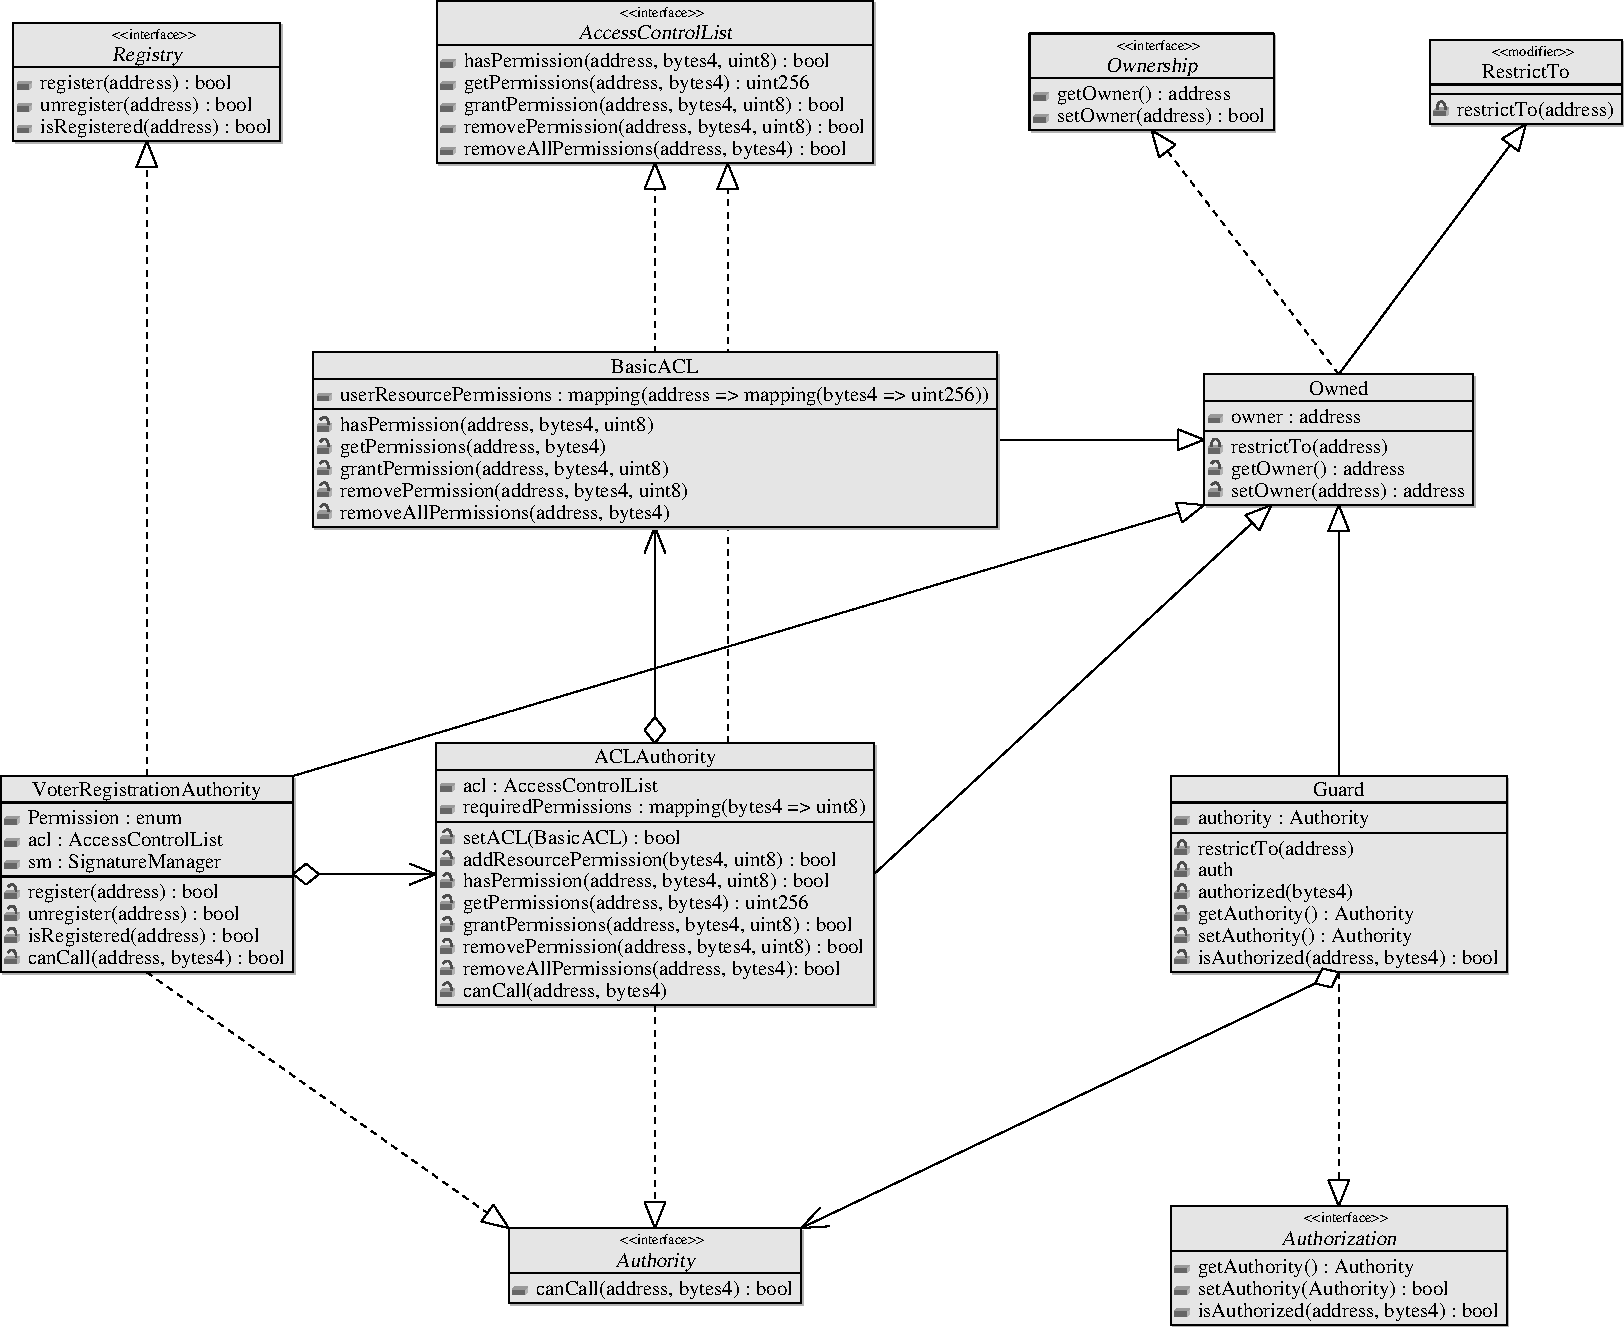
\includegraphics[width=\textwidth]{figures/authorization/figure}
    % \includestandalone[width=\textwidth]{\fig{authorization}}
    \caption{VOI System Architecture~\cite{voi-assessment-report}}\label{fig:voi-architecture}% \label{fig:authorization}
\end{figure}
% cite: Department of Defense Washington Headquarters Services Federal Voting
% cite: https://www.fvap.gov/uploads/FVAP/Reports/voi.pdf
% Assistance Program Voting Over the Internet Pilot Project Assessment Report

\subparagraph{Citizen Infrastructure}
FVAP mailed a CD-ROM to participants containing VOI software, this came in the
form of a Netscape Navigator browser plug-in which provided a graphical user
interface to cast ballots and communicate with the VOI server-side components.
% cite: https://www.fvap.gov/uploads/FVAP/Reports/voi.pdf

% \begin{displayquote}
%   The citizen workstation was the computing platform used by participating
%   citizens to access the Pilot System from their residences or workplaces. The
%   performance requirements for the workstations were intentionally modest to
%   ensure that most existing personal computers would be compatible. The
%   minimum requirements were that the citizen workstation run a Microsoft
%   Windows 95/98 operating system, have a connection to the Internet, and have
%   the Netscape Navigator browser (Version 4.05 or higher, with strong
%   encryption) installed to provide a graphical user interface to the VOI
%   System. Macintosh or UNIX platforms could not be used, nor could Microsoft's
%   Internet Explorer browser. Custom software to enable VOI-specific
%   functionality, in the form of a browser plug-in, was included on a CD-ROM
%   sent to each citizen by the FVAP\@. The CD-ROM also included the strong
%   encryption (128 bit) version of Netscape Navigator for those citizens who
%   needed to upgrade their browser software to be compatible.
% \end{displayquote}

\subparagraph{FVAP Infrastructure}
The FVAP infrastructure consisted of the FVAP server hosting the VOI software,
various networking and power redundancy components to support the server, two
network intrusion detection systems, a server hosting software for creating
electronic ballots, and an administrative workstation for interacting with the
FVAP server. The collective functionalities which this infrastructure provided
included voter authentication, ballot routing to LEO infrastructure, and ballot
creation.

% \begin{displayquote}
% The FVAP server segment was the central component of the VOI System, providing
% the link between the citizen workstations and the LEO servers. The FVAP server
% segment included several different computing platforms, network communication
% components (router, hub), and other components, including a printer, an
% uninterruptible power supply, and a modem for paging system operations and
% maintenance staff. The FVAP segment included the FVAP server, two intrusion
% detection systems, the E-Ballot Tool server, and the FVAP administrative
% workstation.The administrative workstation is a personal computer running a
% Netscape Navigator browser client and is the principal interface to the FVAP
% server for system performance monitoring activities. The two intrusion
% detection system components were positioned on the outside and inside of the
% filtering router to monitor network activities and identify suspicious
% behavior. The intrusion detection system located outside the router is not
% depicted in the system architecture diagram. These two components, along with
% the filtering router and configuration changes to the FVAP server's Microsoft
% Windows NT™ operating system all combined to make the FVAP segment an
% important security barrier protecting the Pilot System.
%
% \emph{FVAP Server}
% The FVAP server included a highly reliable computer hardware server, its
% operating system,database management software, application server software,
% and the VOI custom-developed software. From a functional perspective, the FVAP
% server identified and authenticated users, allowed users to transfer
% Electronic Federal Post Card Applications (EFPCAs) and E-Ballots to and from
% the LEO servers, and performed ``postmarking'' functions. The content of all
% transactions passed through the FVAP server in encrypted form so only the
% addressing information could be read for communications routing purposes.
%
% \emph{E-Ballot Tool Server}
% The E-Ballot Tool server was located within the FVAP server segment security
% architecture and access to it was restricted to specified LEO staff via an
% access control list. This server was dedicated to hosting the E-Ballot Tool
% software. The LEOs used this software to build their electronic ballots. After
% all the component files for the ballots were defined, the LEO would copy those
% associated with a specific ballot style to a floppy disk and upload them to
% the LEO server. No ballots were stored on the E-Ballot Tool server.
% \end{displayquote}

\subparagraph{Local Election Official Infrastructure}
Each LEO site managed a server running VOI software which connected over the
Internet with the FVAP-maintained VOI server and a workstation which allowed
LEOs to perform administrative operations with the server.

% \begin{displayquote}
% Each LEO site had a server that provided connectivity only from the FVAP server
% via the Internet to transmit or receive EFPCAs, E-Ballots, and status messages.
% Each LEO segment included the server hardware platform, the Microsoft Windows NT
% operating system, the VOI custom software, a printer, a removable storage media
% unit, uninterruptible power supply, and network communications devices. Like the
% FVAP segment, each LEO segment had an additional workstation for administration
% of the LEO server.
% \end{displayquote}

% \paragraph{Outcome}
The VOI pilot successfully served 84 volunteers across 4 states. Administrators
did not detect any intrusions into the system during its operation. However, the
DoD acknowledged in their assessment report that one of the major shortcomings
of the pilot was its small sample size, and, that the incentive to attack such a
system would increase as the number of participants
increased.\cite{voi-assessment-report} A future security panel criticized the
VOI system for taking the position that, ``the citizen's workstation is outside
the security perimeter of the system,'' noting that it effectively ignores some
of the most serious kinds of attacks which the system is vulnerable
to.\cite{serve-analysis} On the topic of remote internet voting the DoD
assessment report expressed the following:

\begin{displayquote}[][]
  ``[remote internet voting] is subject to the same security concerns as the
  current VOI System. For this reason, we cannot recommend this alternative as
  an immediate follow-on development to the VOI
  Pilot.\cite{voi-assessment-report}''
\end{displayquote}

%%
% Secure Electronic Registration and Voting Experiment (SERVE) — 2004
%%

\subsubsection{Secure Electronic Registration and Voting Experiment (SERVE) --- 2004}

% In 2002, as directed by Congress and as an immediate follow-on development to
% the VOI pilot, the DoD began work on a remote Internet voting project.

% \subparagraph{Background}
In 2002, following the VOI project, Congress instructed the DoD to carry out a
larger demonstration project, ``under which absent uniformed services voters are
permitted to cast ballots in the regularly scheduled general election for
Federal office.''\cite{serve-bill} To fulfill this mandate FVAP contracted
Accenture to build \emph{The Secure Electronic Registration and Voting
Experiment} (SERVE).

% \paragraph{Objectives and Motivations}
SERVE was built under the United States' Department of Defense's (DoD) Federal
Voting Assistance Program (FVAP) to be deployed for the 2002 or 2004 elections.
Broadly, the motivations behind SERVE were to produce an Internet-based voting
system to reduced barriers to voting for Americans living overseas; specifically
the objectives of the project were to:

\begin{enumerate}
  \item ``assess whether the use of electronic voting technology could improve the
    voting participation success rate for UOCAVA
    citizens,''\cite{dod-expanding-electronic-voting} and

  \item ``assess the potential impact on state and local election administration
    of an automated alternative to the conventional by-mail process of absentee
    registration and voting.''\cite{dod-expanding-electronic-voting}
\end{enumerate}

Fifty counties covering 7 states were targeted for participation and the system was
designed to handle both the registration and voting process.

\paragraph{Architecture}
SERVE shared many architectural-similarities to VOI which are reflected in the
SERVE architecture diagram seen in Figure~\ref{fig:serve-architecture}\@:

\begin{itemize}
  \item SERVE was designed as a web-based service which a voter could connect to
    via web browser.

  \item LEOs managed a local server which could be used to interact with
    the central SERVE system.

  \item The central SERVE system, which performed the bulk of the system
    processing, was maintained by FVAP and stored voter information until the
    appropriate LEO server downloaded it.
\end{itemize}
% to be stored by the central SERVE system that was to be maintained by FVAP\@.

The system was described as consisting of eight integrated subsystems:
Identification and Authentication; Common Services; Voter Registration; Election
Administration; Ballot Definition; Voting; Download and Decryption; and
Tabulation.

\begin{figure}[H]
    \centering
    \includegraphics[width=\textwidth]{03-literature/figures/internet-voting/serve/architecture}
    \caption{SERVE System Architecture~\cite{internet-voting-survey}}\label{fig:serve-architecture}% \label{fig:authorization}
\end{figure}

%  would
% handle identification, registration, authentication, and ballot casting
% procedures. Ballots would be encrypted with LEO  which allowed them to access voter data and encrypted ballots which were

To participate one had to have a military ID (a Common Access Card), or could
enroll in the SERVE system by presenting face-to-face proof of citizenship to a
SERVE official. Once enrolled and registered, a participant could vote via a web
browser through the SERVE site. Figure~\ref{fig:serve-voting-protocol} outlines
the protocol used for casting a ballot through the SERVE web application.

\begin{figure}[H]
    \centering
    \includegraphics[width=0.8\textwidth]{03-literature/figures/internet-voting/serve/protocol}
    \caption{SERVE Voting Protocol~\cite{internet-voting-survey}}\label{fig:serve-voting-protocol}% \label{fig:authorization}
\end{figure}

% \paragraph{Outcome}
SERVE received harsh criticism from independent system reviewers, members of the
\emph{Security Peer Review Group (SPRG)}, academics and industry professionals
who were assembled by FVAP to evaluate the system. A group of these members
independently publicized concerns regarding the security of the system and
Internet-based voting systems more broadly.\cite{serve-analysis}

% \subparagraph{Vulnerabilities}
The report published notes that SERVE suffers from a number of vulnerabilities
and goes into great detail regarding the risks these vulnerabilities pose and
the complexity of performing various attacks to take advantage of these
vulnerabilities. The report noted:\cite{serve-analysis}

\begin{enumerate}
  \item Lack of voter-verified audit trails and vulnerabilities to insider
    attacks. Vulnerabilities in software are difficult to find and intentionally
    obfuscated vulnerabilities are even more so. The essentially unauditable
    nature of electronic voting systems necessitate some form of voter-verified
    audit trail.

  \item Privacy. Several system design issues were identified which would allow
    LEOs or SERVE administrators to tie a ballot to a voter's identity.

  \item Vote Buying/Selling. The nature of Internet voting makes selling
    credentials for voting systems a very real possibility.

  \item Intimidation. Voter intimidation is a problem which all remote voting
    systems must contend with, this problem extends to Internet voting systems.

  \item Large-Scale Impact. Electronic voting machines, if compromised, might
    enable attackers to modify or damage tens or hundreds of thousands of
    ballots. Internet voting systems face this same issue, except on a much
    larger scale; the entire system essentially acts as a single electronic
    voting machine, significantly increasing the scale of impact if compromised.
    Paper-based systems do not face these same exposures.

  \item Too Many Potential Attacks. Electronic systems present a large attack
    surface, exposure to the Internet presents even more. Mitigation of all of
    the kinds of attacks possible would not be feasibility.

  \item Many Sources of Attacks. Elections held over the Internet are vulnerable
    to attacks from around the globe; nation-state entities, terrorists,
    individual hackers and more would all have the ability to attack system.

  \item Undetectable Attacks. Electronic systems make detecting attacks
    extremely difficult and the lack of a detected attack on a system does not
    prove that no attack occurred.

  \item On-screen Electioneering. Many states prevent campaigning within some
    distance of a polling place; however, no such laws exist to prevent ISPs,
    web browsers, or other entities from displaying ads to voters.
\end{enumerate}

% The details of the vulnerabilities reported
% are discussed in further detail in Section~\ref{section:shared-weaknesses},
% however, the report notes:

In addition the report had this to say about future attempts at building
Internet voting systems:

\begin{displayquote}
  ``Like the proponents of SERVE, we believe that there should be better support
  for voting for our military overseas. Still, we regret that we are forced to
  conclude that the best course is not to field the SERVE system at all. Because
  the danger of successful, large-scale attacks is so great, we reluctantly
  recommend shutting down the development of SERVE immediately and not
  attempting anything like it in the future until both the Internet and the
  world's home computer infrastructure have been fundamentally redesigned, or
  some other unforeseen security breakthroughs appear.''\cite{serve-analysis}
\end{displayquote}

In response to these criticisms and concerns documented in this report, the
then-Deputy Secretary of Defense Paul Wolfowitz decided that the SERVE project
would not go forward as planned for the 2004 election, effectively killing the
project.\cite{dod-expanding-electronic-voting} Three years later the DoD
published a report which downplayed the criticisms and concerns published by the
SPRG members.\cite{dod-expanding-electronic-voting} In reaction to this DoD
report, the members of the SPRG independently publicized a response which
criticized the report for downplaying the concerns laid out in their initial
security analysis of SERVE, and further reiterated their concerns regarding
Internet voting. The members of the SPRG noted again that the issues faced by
SERVE are ones which are not capable of being fixed by a better design or
architecture of Internet voting systems, because the fundamental issues are ones
which could only be fixed by redesigning both the Internet and personal
computers.\cite{comment-on-dod-report}

% \subsubsection{Integrated Voting Alternative Site (IVAS)}
% September 2006

% Interim Voting Assistance System
% https://graphics8.nytimes.com/packages/pdf/national/2006_IVAS_report.pdf

% Integrated Voting Alternative Site
% https://www.fvap.gov/uploads/FVAP/Reports/ivas06.pdf
% \todo{What does IVAS stand for? A: It stands for both.}
% \todo{Complete section.}

\subsubsection{D.C. Digital Vote-by-Mail System (DVBM) --- 2010}

% \subparagraph{Background}
In 2009 the \emph{Military and Overseas Voter Empowerment Act (MOVE)} was
passed. This act amended UOCAVA and other statutes to provide further protections
to eligible citizens. Specifically the act aimed to reduce the number of ballots
which are not counted due to late receipt. MOVE accomplishes this by requiring
that states send absentee ballots no later that 45 days prior to election day.
MOVE goes further by requiring that all registration material and blank ballots
be available electronically and removes requirements regarding notarization on
voting applications and ballots.\cite{MOVE}

% \begin{displayquote}
%   In 2010, Washington, D.C.\ developed an Internet voting pilot project that was
%   intended to allow overseas absentee voters to cast their ballots using a
%   website.
%   % https://jhalderm.com/pub/papers/dcvoting-fc12.pdf
% \end{displayquote}

% \paragraph{Objectives and Motivations}
In search of a solution to improve their compliance with the MOVE act,
Washington's District of Columbia Board of Elections and Ethics (DCBOEE/BOEE)
planned to launch an Internet voting system, the D.C. Digital Vote-by-Mail
(DVBM) system, for use in the November 2010 general election. The project was
developed in partnership with the Open Source Digital Voting (OSDV) Foundation's
TrustTheVote project, who viewed the project as a mostly academic
effort.\cite{trust-the-vote-dc-pilot} The system was slated to be operational in
time for the November 2010 general election and aimed to provide two primary
functionalities:\cite{internet-voting-survey,dc-voting-system}
\begin{enumerate}
  \item allow voters to electronically access voting materials
  \item allow voters to optionally cast their ballot over the internet
\end{enumerate}

% \paragraph{Architecture}
The DVBM architecture, illustrated in Figure~\ref{fig:dvbm-architecture}, was
developed as a web application using the Ruby on Rails framework; was hosted
using the Apache web server; used MySQL as its database technology, which stored
the global election state (voters' names, addresses, etc.); and used the
underlying (Linux) filesystem to store encrypted ballots cast by voters. When
the voting phase of the election was complete, election officials would transfer
the encrypted ballots to an air-gapped computer for decryption and printing.
Printed ballots would be counted alongside other mail-in absentee
ballots.\cite{dc-voting-system}

\begin{figure}[H]
    \centering
    \includegraphics[width=\textwidth]{03-literature/figures/internet-voting/dc/architecture}
    % \includesvg[width=\textwidth]{03-literature/figures/internet-voting/voi/voi.svg}
    % \input{03-literature/figures/internet-voting/voi/voi2.pdf_tex}
    % 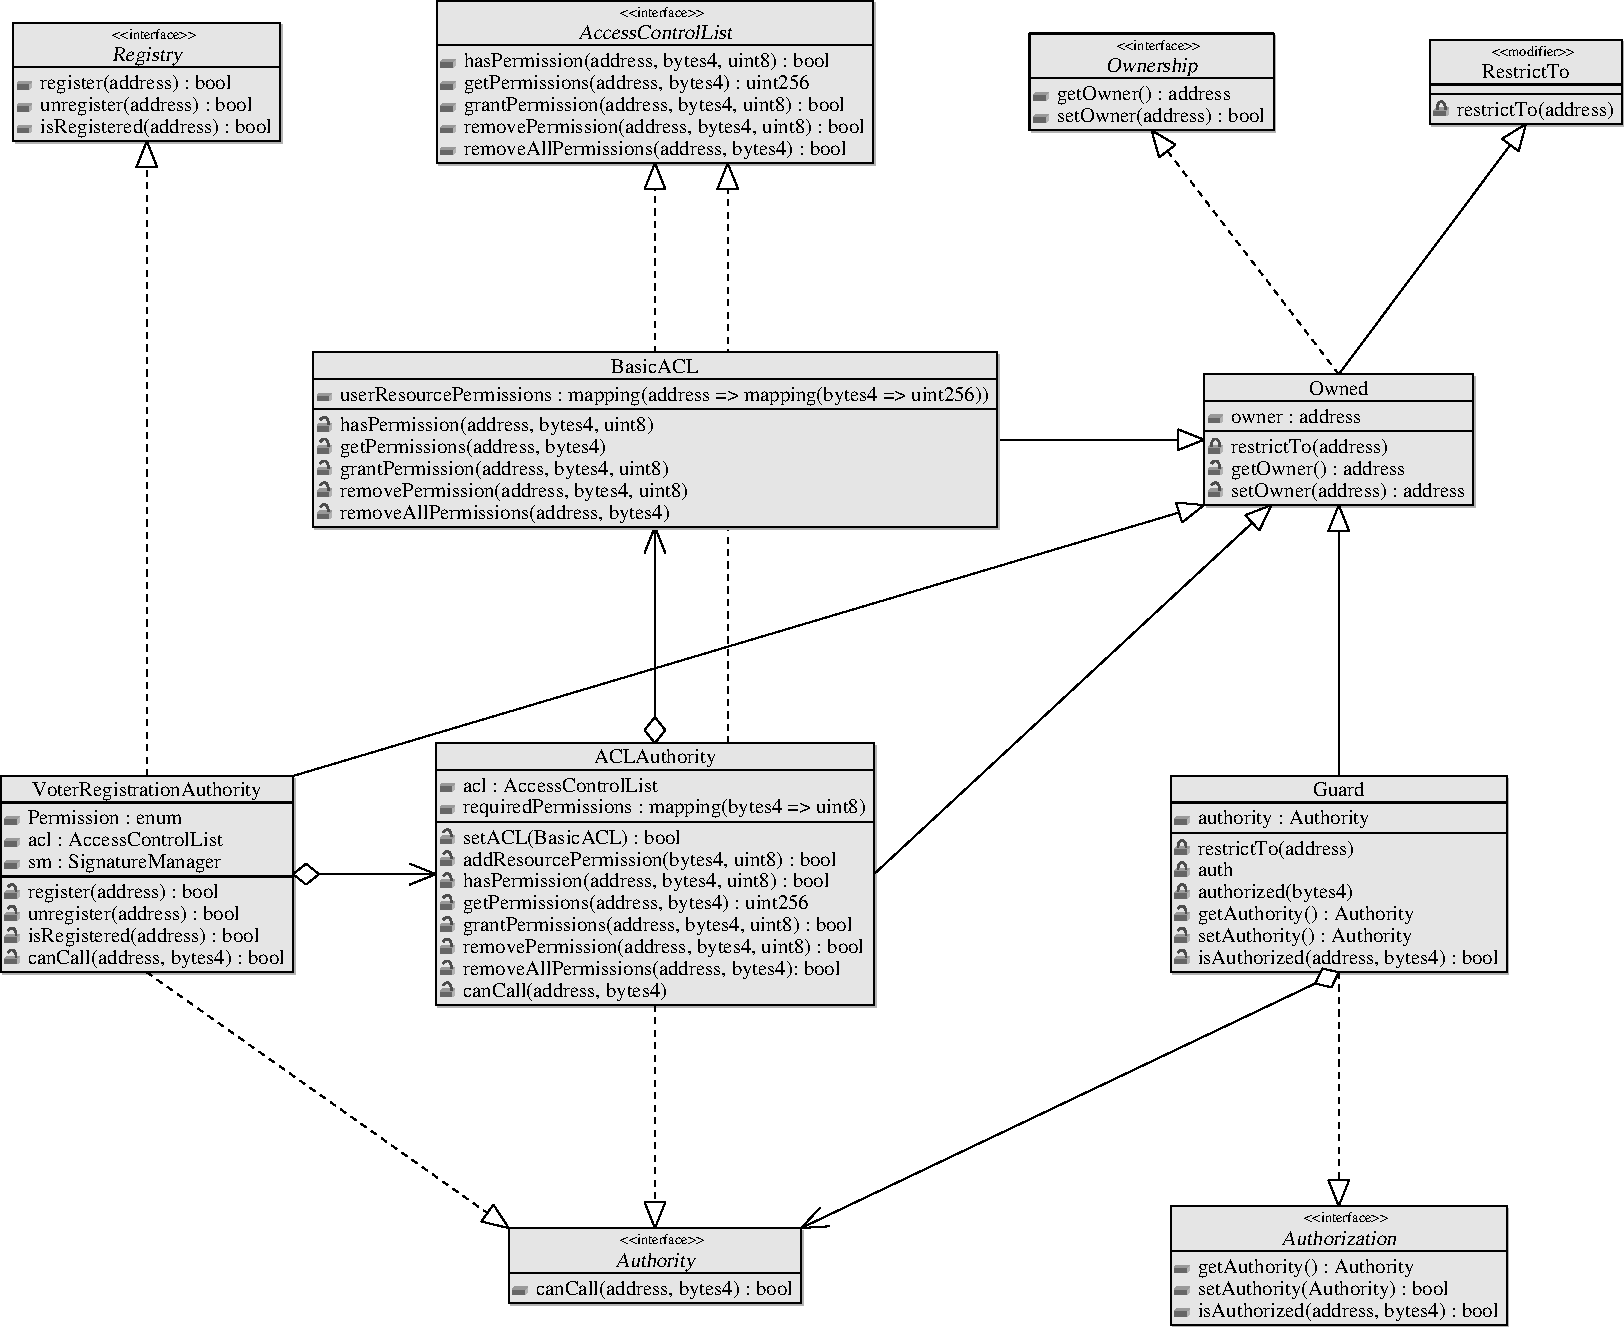
\includegraphics[width=\textwidth]{figures/authorization/figure}
    % \includestandalone[width=\textwidth]{\fig{authorization}}
    \caption{DVBM System Architecture~\cite{dc-voting-system}}\label{fig:dvbm-architecture}% \label{fig:authorization}
\end{figure}

Prior to the official launch of the system the BOEE opted to conduct a mock
election where members of the public, researchers, and hackers alike were
invited to to test the functionality of the system, discover vulnerabilities,
and attempt to compromise the security, reliability, and availability of the
system.\cite{internet-voting-survey,dc-voting-system,trust-the-vote-dc-pilot}

% \paragraph{Outcome}
Within 48 hours of the system going live researchers from The University of
Michigan, playing the role of an attacker, demonstrated a number of
vulnerabilities and attacks on on the system and managed to gained near-complete
control of the election server. Their intrusion was not detected for nearly 2
days.\cite{dc-voting-system}
% Prior to its launch election officials held a mock election to test the security
% of the system, inviting researchers and hackers alike to attempt to compromise
% the security, reliability, and availability of the system. A number of attacks
% were demonstrated and researchers were able to:

Demonstrated vulnerabilities included being able to:
\begin{itemize}
  \item penetrate the network of the election software
  \item determine voter's identities
  \item locate unencrypted ballots, thus mapping voter's identities to their
    personal votes
  \item modify ballots
  \item cast fake ballots
  \item modify the election system software itself
\end{itemize}

Once election officials became aware of the attack, the mock election was
suspended, five days ahead of schedule, citing ``usability issues.'' Election
officials later confirmed that they were unable to detect the attack or network
presence using their intrusion detection system. Due to the test results, the
portion of the system which allowed for ballots to be submitted over the
Internet was not used.\cite{dc-voting-system}

\subsubsection{Estonia --- 2005}
Estonia began using Internet voting in 2005\cite{internet-voting-survey}; in the
2015 Estonian parliamentary elections, 30.5\% of all voters voted over the
Internet. Estonia maintains what is likely the most advanced national
identification cards in the world. Estonian IDs are part of a \emph{Public Key
Infrastructure (PKI)} where IDs serve as smart cards which possess two RSA key
pairs: one for signing and one for authentication; these cryptographic functions
are performed directly on the card. The signatures produced by these IDs are
used extensively throughout the country and are considered legally binding.
These cryptographic IDs allow Estonia to provide voter authentication
capabilities that cannot be reproduced in the US.\ Despite the advanced
authentication capabilities that Estonia is able to achieve, researchers in 2014
devised a number of attacks that could be performed on the Estonian voting
system to spoil ballots, damage ballot secrecy, and steal or drop votes. The
researchers also criticized the transparency and operational security of the
system, noting that videos of the administration processes --- provided for
transparency purposes --- recorded administrators entering root passwords,
revealed network credentials which had been posted on a wall, and showed
administrators using USB drives containing personal files to move sensitive
election materials between systems.\cite{estonia}

% \subsection{Shared Weaknesses}\label{section:shared-weaknesses}
% There are a number of shared weaknesses and vulnerabilities exposed across these
% internet voting systems which the systems incur due to the underlying
% architecture of the systems, their Internet, the personal computer, and remote
% voting.
%
% \begin{enumerate}
%   \item Lack of voter-verified audit trails.
%   \item Vulnerabilities to insider attacks.
%   \item Privacy.
%   \item Vote Buying/Selling.
%   \item Intimidation.
%   \item Large-Scale Impact.
%   \item Too Many Potential Attacks.
%   \item Many Sources of Attacks.
%   \item Undetectable Attacks.
%   \item On-screen Electioneering.
% \end{enumerate}

% \todo{
%   Should I add a shared weaknesses section here and remove some of the
%   demonstrated attacks from the individual systems?
% }


% Section: Internet Voting
\section{Internet Voting}\label{sec:internet-voting}
Internet voting, sometimes referred to as \emph{remote electronic voting}, is a
system of voting where voters are able to cast their votes over the Internet.

% \subsection{Procedure}
% \todo{
%   This doesn't need to be a subsection, just mention it at the start of the
%   Internet Voting section.
% }
\paragraph{Procedure}
The U.S.\ Vote Foundation describes the typical phases involved in conducting an
Internet based election as follows:\cite{e2e-viv}

\begin{enumerate}
  \item \emph{Setup}, during which election officials gather voter information,
    identify election issues and races, design ballots, etc.

  \item \emph{Distribution}, during which election materials are distributed to
    voters: ballots, credentials, voting instructions, etc.

  \item \emph{Voting}, during which voters mark their ballots.

  \item \emph{Casting}, where voters finalize and submit their ballots and
    election officials receive said ballots.

  \item \emph{Tallying}, where election officials count votes, tabulate results,
    and announce winners.

  \item \emph{Auditing}, where (as necessary) vote results are evaluated for
    incorrect results.
\end{enumerate}
% \todo{cite: The Future of Voting — Chapter 3.1}
% cite: The Future of Voting - Chapter 3.1

% \subsection{Requirements}
\paragraph{Requirements}
The requirements for an Internet-based voting system are the same as those for
any other voting system; it must be \emph{secure}, \emph{correct}, and
\emph{private}.
% \todo{Complete section.}

\subsection{Survey of Internet Voting Systems}

In September of 2011 the \emph{Election Assistance Commission (EAC)} published
\emph{``A Survey of Internet Voting,''} which offered a broad review of various
Internet voting systems used between the years of 2000 and
2011.\cite{internet-voting-survey} In total, the survey reviews 30 Internet
voting systems used for elections and primaries, by various parties and
governments, at various levels of government: national, state, and local.

% The survey defines internet voting as,
%
% \begin{displayquote}
%   any system where the voter's ballot selections are transmitted over the
%   Internet from a location other than a polling place to the entity conducting
%   the election.
% \end{displayquote}

% cite: A Survey of Internet Voting Systems - EAC
% https://www.eac.gov/sites/default/files/eac_assets/1/28/SIV-FINAL.pdf

% \begin{description}[style=multiline,font=\normalfont,leftmargin=2cm]
%   \item[2000] Alaska sponsored by the Democratic National Party,
%   \item[2000] Arizona 2000 by the Arizona Democratic Party, and
%   \item[2000] VOI by the FVAP,
%
%   \item[2004] Michigan by the Michigan Democratic Party,
%   \item[2004] SERVE by the FVAP,
%
%   \item[2005/2007/2009/2011] Estonia,
%
%   \item[2008] Democrats Abroad by Democrats Abroad,
%   \item[2008/2010] Arizona 2008/2010 by Arizona Secretary of State's Office,
%   \item[2008] ODBP by Okaloosa County Supervisor of Elections,
%
%   \item[2009] Honolulu by the City of Honolulu,
%
%   \item[2010] District of Columbia by the DC Board of Elections and Ethics,
%   \item[2010] Oregon by the Independent Party of Oregon,
%   \item[2010] West Virginia by the West Virginia Secretary of State,
% \end{description}

\subsubsection{Voting Over the Internet (VOI) --- 2000}

% \subparagraph{Background}
In 1986, the \emph{Uniformed and Overseas Citizens Absentee Voting Act (UOCAVA)}
was passed to render services to merchant marines, uniformed services, and other
overseas civilians. Broadly, UOCAVA mandates that overseas and military
voters be able to remotely register and vote in federal elections, and
designates the Secretary of Defense as the executive agent responsible for
implementing its provisions. Thus, under the \emph{Department of Defense
(DoD)}, the \emph{Federal Voting Assistance Program (FVAP)} was established  to
provide voter assistance, tools, and education to overseas voters with the goal
of enabling overseas voters to vote from anywhere in the world. In pursuit of
this goal, FVAP established procedures for delivering election materials through
domestic, military, and foreign postal systems.

% \paragraph{Objectives and Motivations}
In an effort to eliminate some of the weaknesses inherit in postal systems,
primarily transit times and unreliable delivery guarantees, FVAP established the
\emph{Voting Over the Internet (VOI)} project.

\begin{displayquote}
  ``The pilot project was designed to examine the feasibility of using the
  Internet for remote registration and voting in an effort to overcome the time
  and distance barriers faced by UOCAVA voters. `This was the first time that
  binding votes were cast over the Internet for federal, state, and local
  offices, including the President and Members of
  Congress.'{}''\cite{internet-voting-survey,voi-assessment-report}
\end{displayquote}
% cite: A Survey of Internet Voting Systems - EAC

% \paragraph{Architecture}
The VOI architecture consisted of 3 major components, as illustrated in
Figure~\ref{fig:voi-architecture}:

\begin{itemize}
  \item Citizen infrastructure: any workstation or personal computer with
    Internet access that was available to the voter.

  \item FVAP infrastructure: VOI systems maintained by FVAP, namely the FVAP
    server, which hosted the server-side VOI software, various intrusion
    detection systems, networking infrastructure, and administrative
    workstations.

  \item Local Election Official (LEO) infrastructure: systems managed by
    LEOs, namely servers running VOI software and workstations to interact with
    said software.
\end{itemize}

\begin{figure}[H]
    \centering
    \includegraphics[width=\textwidth]{03-literature/figures/internet-voting/voi/voip}
    % \includesvg[width=\textwidth]{03-literature/figures/internet-voting/voi/voi.svg}
    % \input{03-literature/figures/internet-voting/voi/voi2.pdf_tex}
    % 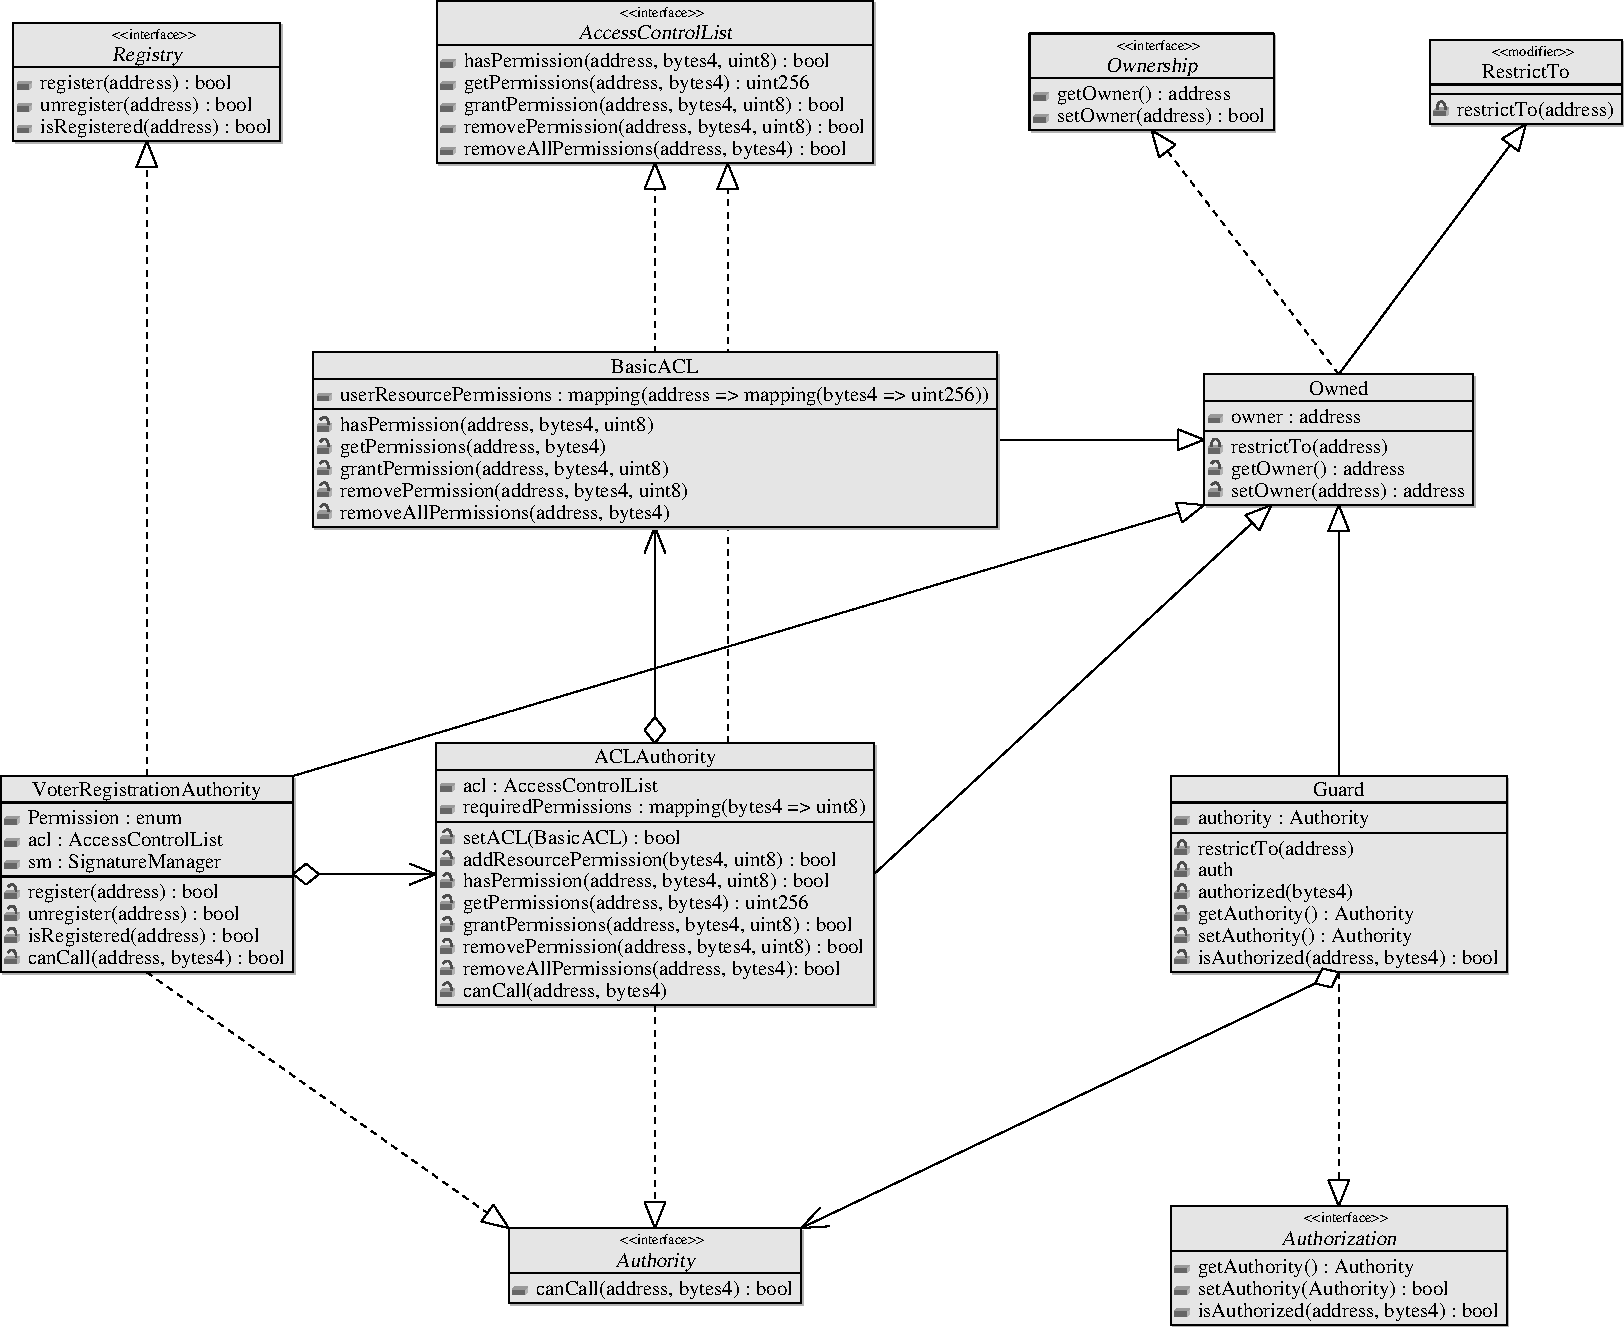
\includegraphics[width=\textwidth]{figures/authorization/figure}
    % \includestandalone[width=\textwidth]{\fig{authorization}}
    \caption{VOI System Architecture~\cite{voi-assessment-report}}\label{fig:voi-architecture}% \label{fig:authorization}
\end{figure}
% cite: Department of Defense Washington Headquarters Services Federal Voting
% cite: https://www.fvap.gov/uploads/FVAP/Reports/voi.pdf
% Assistance Program Voting Over the Internet Pilot Project Assessment Report

\subparagraph{Citizen Infrastructure}
FVAP mailed a CD-ROM to participants containing VOI software, this came in the
form of a Netscape Navigator browser plug-in which provided a graphical user
interface to cast ballots and communicate with the VOI server-side components.
% cite: https://www.fvap.gov/uploads/FVAP/Reports/voi.pdf

% \begin{displayquote}
%   The citizen workstation was the computing platform used by participating
%   citizens to access the Pilot System from their residences or workplaces. The
%   performance requirements for the workstations were intentionally modest to
%   ensure that most existing personal computers would be compatible. The
%   minimum requirements were that the citizen workstation run a Microsoft
%   Windows 95/98 operating system, have a connection to the Internet, and have
%   the Netscape Navigator browser (Version 4.05 or higher, with strong
%   encryption) installed to provide a graphical user interface to the VOI
%   System. Macintosh or UNIX platforms could not be used, nor could Microsoft's
%   Internet Explorer browser. Custom software to enable VOI-specific
%   functionality, in the form of a browser plug-in, was included on a CD-ROM
%   sent to each citizen by the FVAP\@. The CD-ROM also included the strong
%   encryption (128 bit) version of Netscape Navigator for those citizens who
%   needed to upgrade their browser software to be compatible.
% \end{displayquote}

\subparagraph{FVAP Infrastructure}
The FVAP infrastructure consisted of the FVAP server hosting the VOI software,
various networking and power redundancy components to support the server, two
network intrusion detection systems, a server hosting software for creating
electronic ballots, and an administrative workstation for interacting with the
FVAP server. The collective functionalities which this infrastructure provided
included voter authentication, ballot routing to LEO infrastructure, and ballot
creation.

% \begin{displayquote}
% The FVAP server segment was the central component of the VOI System, providing
% the link between the citizen workstations and the LEO servers. The FVAP server
% segment included several different computing platforms, network communication
% components (router, hub), and other components, including a printer, an
% uninterruptible power supply, and a modem for paging system operations and
% maintenance staff. The FVAP segment included the FVAP server, two intrusion
% detection systems, the E-Ballot Tool server, and the FVAP administrative
% workstation.The administrative workstation is a personal computer running a
% Netscape Navigator browser client and is the principal interface to the FVAP
% server for system performance monitoring activities. The two intrusion
% detection system components were positioned on the outside and inside of the
% filtering router to monitor network activities and identify suspicious
% behavior. The intrusion detection system located outside the router is not
% depicted in the system architecture diagram. These two components, along with
% the filtering router and configuration changes to the FVAP server's Microsoft
% Windows NT™ operating system all combined to make the FVAP segment an
% important security barrier protecting the Pilot System.
%
% \emph{FVAP Server}
% The FVAP server included a highly reliable computer hardware server, its
% operating system,database management software, application server software,
% and the VOI custom-developed software. From a functional perspective, the FVAP
% server identified and authenticated users, allowed users to transfer
% Electronic Federal Post Card Applications (EFPCAs) and E-Ballots to and from
% the LEO servers, and performed ``postmarking'' functions. The content of all
% transactions passed through the FVAP server in encrypted form so only the
% addressing information could be read for communications routing purposes.
%
% \emph{E-Ballot Tool Server}
% The E-Ballot Tool server was located within the FVAP server segment security
% architecture and access to it was restricted to specified LEO staff via an
% access control list. This server was dedicated to hosting the E-Ballot Tool
% software. The LEOs used this software to build their electronic ballots. After
% all the component files for the ballots were defined, the LEO would copy those
% associated with a specific ballot style to a floppy disk and upload them to
% the LEO server. No ballots were stored on the E-Ballot Tool server.
% \end{displayquote}

\subparagraph{Local Election Official Infrastructure}
Each LEO site managed a server running VOI software which connected over the
Internet with the FVAP-maintained VOI server and a workstation which allowed
LEOs to perform administrative operations with the server.

% \begin{displayquote}
% Each LEO site had a server that provided connectivity only from the FVAP server
% via the Internet to transmit or receive EFPCAs, E-Ballots, and status messages.
% Each LEO segment included the server hardware platform, the Microsoft Windows NT
% operating system, the VOI custom software, a printer, a removable storage media
% unit, uninterruptible power supply, and network communications devices. Like the
% FVAP segment, each LEO segment had an additional workstation for administration
% of the LEO server.
% \end{displayquote}

% \paragraph{Outcome}
The VOI pilot successfully served 84 volunteers across 4 states. Administrators
did not detect any intrusions into the system during its operation. However, the
DoD acknowledged in their assessment report that one of the major shortcomings
of the pilot was its small sample size, and, that the incentive to attack such a
system would increase as the number of participants
increased.\cite{voi-assessment-report} A future security panel criticized the
VOI system for taking the position that, ``the citizen's workstation is outside
the security perimeter of the system,'' noting that it effectively ignores some
of the most serious kinds of attacks which the system is vulnerable
to.\cite{serve-analysis} On the topic of remote internet voting the DoD
assessment report expressed the following:

\begin{displayquote}[][]
  ``[remote internet voting] is subject to the same security concerns as the
  current VOI System. For this reason, we cannot recommend this alternative as
  an immediate follow-on development to the VOI
  Pilot.\cite{voi-assessment-report}''
\end{displayquote}

%%
% Secure Electronic Registration and Voting Experiment (SERVE) — 2004
%%

\subsubsection{Secure Electronic Registration and Voting Experiment (SERVE) --- 2004}

% In 2002, as directed by Congress and as an immediate follow-on development to
% the VOI pilot, the DoD began work on a remote Internet voting project.

% \subparagraph{Background}
In 2002, following the VOI project, Congress instructed the DoD to carry out a
larger demonstration project, ``under which absent uniformed services voters are
permitted to cast ballots in the regularly scheduled general election for
Federal office.''\cite{serve-bill} To fulfill this mandate FVAP contracted
Accenture to build \emph{The Secure Electronic Registration and Voting
Experiment} (SERVE).

% \paragraph{Objectives and Motivations}
SERVE was built under the United States' Department of Defense's (DoD) Federal
Voting Assistance Program (FVAP) to be deployed for the 2002 or 2004 elections.
Broadly, the motivations behind SERVE were to produce an Internet-based voting
system to reduced barriers to voting for Americans living overseas; specifically
the objectives of the project were to:

\begin{enumerate}
  \item ``assess whether the use of electronic voting technology could improve the
    voting participation success rate for UOCAVA
    citizens,''\cite{dod-expanding-electronic-voting} and

  \item ``assess the potential impact on state and local election administration
    of an automated alternative to the conventional by-mail process of absentee
    registration and voting.''\cite{dod-expanding-electronic-voting}
\end{enumerate}

Fifty counties covering 7 states were targeted for participation and the system was
designed to handle both the registration and voting process.

\paragraph{Architecture}
SERVE shared many architectural-similarities to VOI which are reflected in the
SERVE architecture diagram seen in Figure~\ref{fig:serve-architecture}\@:

\begin{itemize}
  \item SERVE was designed as a web-based service which a voter could connect to
    via web browser.

  \item LEOs managed a local server which could be used to interact with
    the central SERVE system.

  \item The central SERVE system, which performed the bulk of the system
    processing, was maintained by FVAP and stored voter information until the
    appropriate LEO server downloaded it.
\end{itemize}
% to be stored by the central SERVE system that was to be maintained by FVAP\@.

The system was described as consisting of eight integrated subsystems:
Identification and Authentication; Common Services; Voter Registration; Election
Administration; Ballot Definition; Voting; Download and Decryption; and
Tabulation.

\begin{figure}[H]
    \centering
    \includegraphics[width=\textwidth]{03-literature/figures/internet-voting/serve/architecture}
    \caption{SERVE System Architecture~\cite{internet-voting-survey}}\label{fig:serve-architecture}% \label{fig:authorization}
\end{figure}

%  would
% handle identification, registration, authentication, and ballot casting
% procedures. Ballots would be encrypted with LEO  which allowed them to access voter data and encrypted ballots which were

To participate one had to have a military ID (a Common Access Card), or could
enroll in the SERVE system by presenting face-to-face proof of citizenship to a
SERVE official. Once enrolled and registered, a participant could vote via a web
browser through the SERVE site. Figure~\ref{fig:serve-voting-protocol} outlines
the protocol used for casting a ballot through the SERVE web application.

\begin{figure}[H]
    \centering
    \includegraphics[width=0.8\textwidth]{03-literature/figures/internet-voting/serve/protocol}
    \caption{SERVE Voting Protocol~\cite{internet-voting-survey}}\label{fig:serve-voting-protocol}% \label{fig:authorization}
\end{figure}

% \paragraph{Outcome}
SERVE received harsh criticism from independent system reviewers, members of the
\emph{Security Peer Review Group (SPRG)}, academics and industry professionals
who were assembled by FVAP to evaluate the system. A group of these members
independently publicized concerns regarding the security of the system and
Internet-based voting systems more broadly.\cite{serve-analysis}

% \subparagraph{Vulnerabilities}
The report published notes that SERVE suffers from a number of vulnerabilities
and goes into great detail regarding the risks these vulnerabilities pose and
the complexity of performing various attacks to take advantage of these
vulnerabilities. The report noted:\cite{serve-analysis}

\begin{enumerate}
  \item Lack of voter-verified audit trails and vulnerabilities to insider
    attacks. Vulnerabilities in software are difficult to find and intentionally
    obfuscated vulnerabilities are even more so. The essentially unauditable
    nature of electronic voting systems necessitate some form of voter-verified
    audit trail.

  \item Privacy. Several system design issues were identified which would allow
    LEOs or SERVE administrators to tie a ballot to a voter's identity.

  \item Vote Buying/Selling. The nature of Internet voting makes selling
    credentials for voting systems a very real possibility.

  \item Intimidation. Voter intimidation is a problem which all remote voting
    systems must contend with, this problem extends to Internet voting systems.

  \item Large-Scale Impact. Electronic voting machines, if compromised, might
    enable attackers to modify or damage tens or hundreds of thousands of
    ballots. Internet voting systems face this same issue, except on a much
    larger scale; the entire system essentially acts as a single electronic
    voting machine, significantly increasing the scale of impact if compromised.
    Paper-based systems do not face these same exposures.

  \item Too Many Potential Attacks. Electronic systems present a large attack
    surface, exposure to the Internet presents even more. Mitigation of all of
    the kinds of attacks possible would not be feasibility.

  \item Many Sources of Attacks. Elections held over the Internet are vulnerable
    to attacks from around the globe; nation-state entities, terrorists,
    individual hackers and more would all have the ability to attack system.

  \item Undetectable Attacks. Electronic systems make detecting attacks
    extremely difficult and the lack of a detected attack on a system does not
    prove that no attack occurred.

  \item On-screen Electioneering. Many states prevent campaigning within some
    distance of a polling place; however, no such laws exist to prevent ISPs,
    web browsers, or other entities from displaying ads to voters.
\end{enumerate}

% The details of the vulnerabilities reported
% are discussed in further detail in Section~\ref{section:shared-weaknesses},
% however, the report notes:

In addition the report had this to say about future attempts at building
Internet voting systems:

\begin{displayquote}
  ``Like the proponents of SERVE, we believe that there should be better support
  for voting for our military overseas. Still, we regret that we are forced to
  conclude that the best course is not to field the SERVE system at all. Because
  the danger of successful, large-scale attacks is so great, we reluctantly
  recommend shutting down the development of SERVE immediately and not
  attempting anything like it in the future until both the Internet and the
  world's home computer infrastructure have been fundamentally redesigned, or
  some other unforeseen security breakthroughs appear.''\cite{serve-analysis}
\end{displayquote}

In response to these criticisms and concerns documented in this report, the
then-Deputy Secretary of Defense Paul Wolfowitz decided that the SERVE project
would not go forward as planned for the 2004 election, effectively killing the
project.\cite{dod-expanding-electronic-voting} Three years later the DoD
published a report which downplayed the criticisms and concerns published by the
SPRG members.\cite{dod-expanding-electronic-voting} In reaction to this DoD
report, the members of the SPRG independently publicized a response which
criticized the report for downplaying the concerns laid out in their initial
security analysis of SERVE, and further reiterated their concerns regarding
Internet voting. The members of the SPRG noted again that the issues faced by
SERVE are ones which are not capable of being fixed by a better design or
architecture of Internet voting systems, because the fundamental issues are ones
which could only be fixed by redesigning both the Internet and personal
computers.\cite{comment-on-dod-report}

% \subsubsection{Integrated Voting Alternative Site (IVAS)}
% September 2006

% Interim Voting Assistance System
% https://graphics8.nytimes.com/packages/pdf/national/2006_IVAS_report.pdf

% Integrated Voting Alternative Site
% https://www.fvap.gov/uploads/FVAP/Reports/ivas06.pdf
% \todo{What does IVAS stand for? A: It stands for both.}
% \todo{Complete section.}

\subsubsection{D.C. Digital Vote-by-Mail System (DVBM) --- 2010}

% \subparagraph{Background}
In 2009 the \emph{Military and Overseas Voter Empowerment Act (MOVE)} was
passed. This act amended UOCAVA and other statutes to provide further protections
to eligible citizens. Specifically the act aimed to reduce the number of ballots
which are not counted due to late receipt. MOVE accomplishes this by requiring
that states send absentee ballots no later that 45 days prior to election day.
MOVE goes further by requiring that all registration material and blank ballots
be available electronically and removes requirements regarding notarization on
voting applications and ballots.\cite{MOVE}

% \begin{displayquote}
%   In 2010, Washington, D.C.\ developed an Internet voting pilot project that was
%   intended to allow overseas absentee voters to cast their ballots using a
%   website.
%   % https://jhalderm.com/pub/papers/dcvoting-fc12.pdf
% \end{displayquote}

% \paragraph{Objectives and Motivations}
In search of a solution to improve their compliance with the MOVE act,
Washington's District of Columbia Board of Elections and Ethics (DCBOEE/BOEE)
planned to launch an Internet voting system, the D.C. Digital Vote-by-Mail
(DVBM) system, for use in the November 2010 general election. The project was
developed in partnership with the Open Source Digital Voting (OSDV) Foundation's
TrustTheVote project, who viewed the project as a mostly academic
effort.\cite{trust-the-vote-dc-pilot} The system was slated to be operational in
time for the November 2010 general election and aimed to provide two primary
functionalities:\cite{internet-voting-survey,dc-voting-system}
\begin{enumerate}
  \item allow voters to electronically access voting materials
  \item allow voters to optionally cast their ballot over the internet
\end{enumerate}

% \paragraph{Architecture}
The DVBM architecture, illustrated in Figure~\ref{fig:dvbm-architecture}, was
developed as a web application using the Ruby on Rails framework; was hosted
using the Apache web server; used MySQL as its database technology, which stored
the global election state (voters' names, addresses, etc.); and used the
underlying (Linux) filesystem to store encrypted ballots cast by voters. When
the voting phase of the election was complete, election officials would transfer
the encrypted ballots to an air-gapped computer for decryption and printing.
Printed ballots would be counted alongside other mail-in absentee
ballots.\cite{dc-voting-system}

\begin{figure}[H]
    \centering
    \includegraphics[width=\textwidth]{03-literature/figures/internet-voting/dc/architecture}
    % \includesvg[width=\textwidth]{03-literature/figures/internet-voting/voi/voi.svg}
    % \input{03-literature/figures/internet-voting/voi/voi2.pdf_tex}
    % 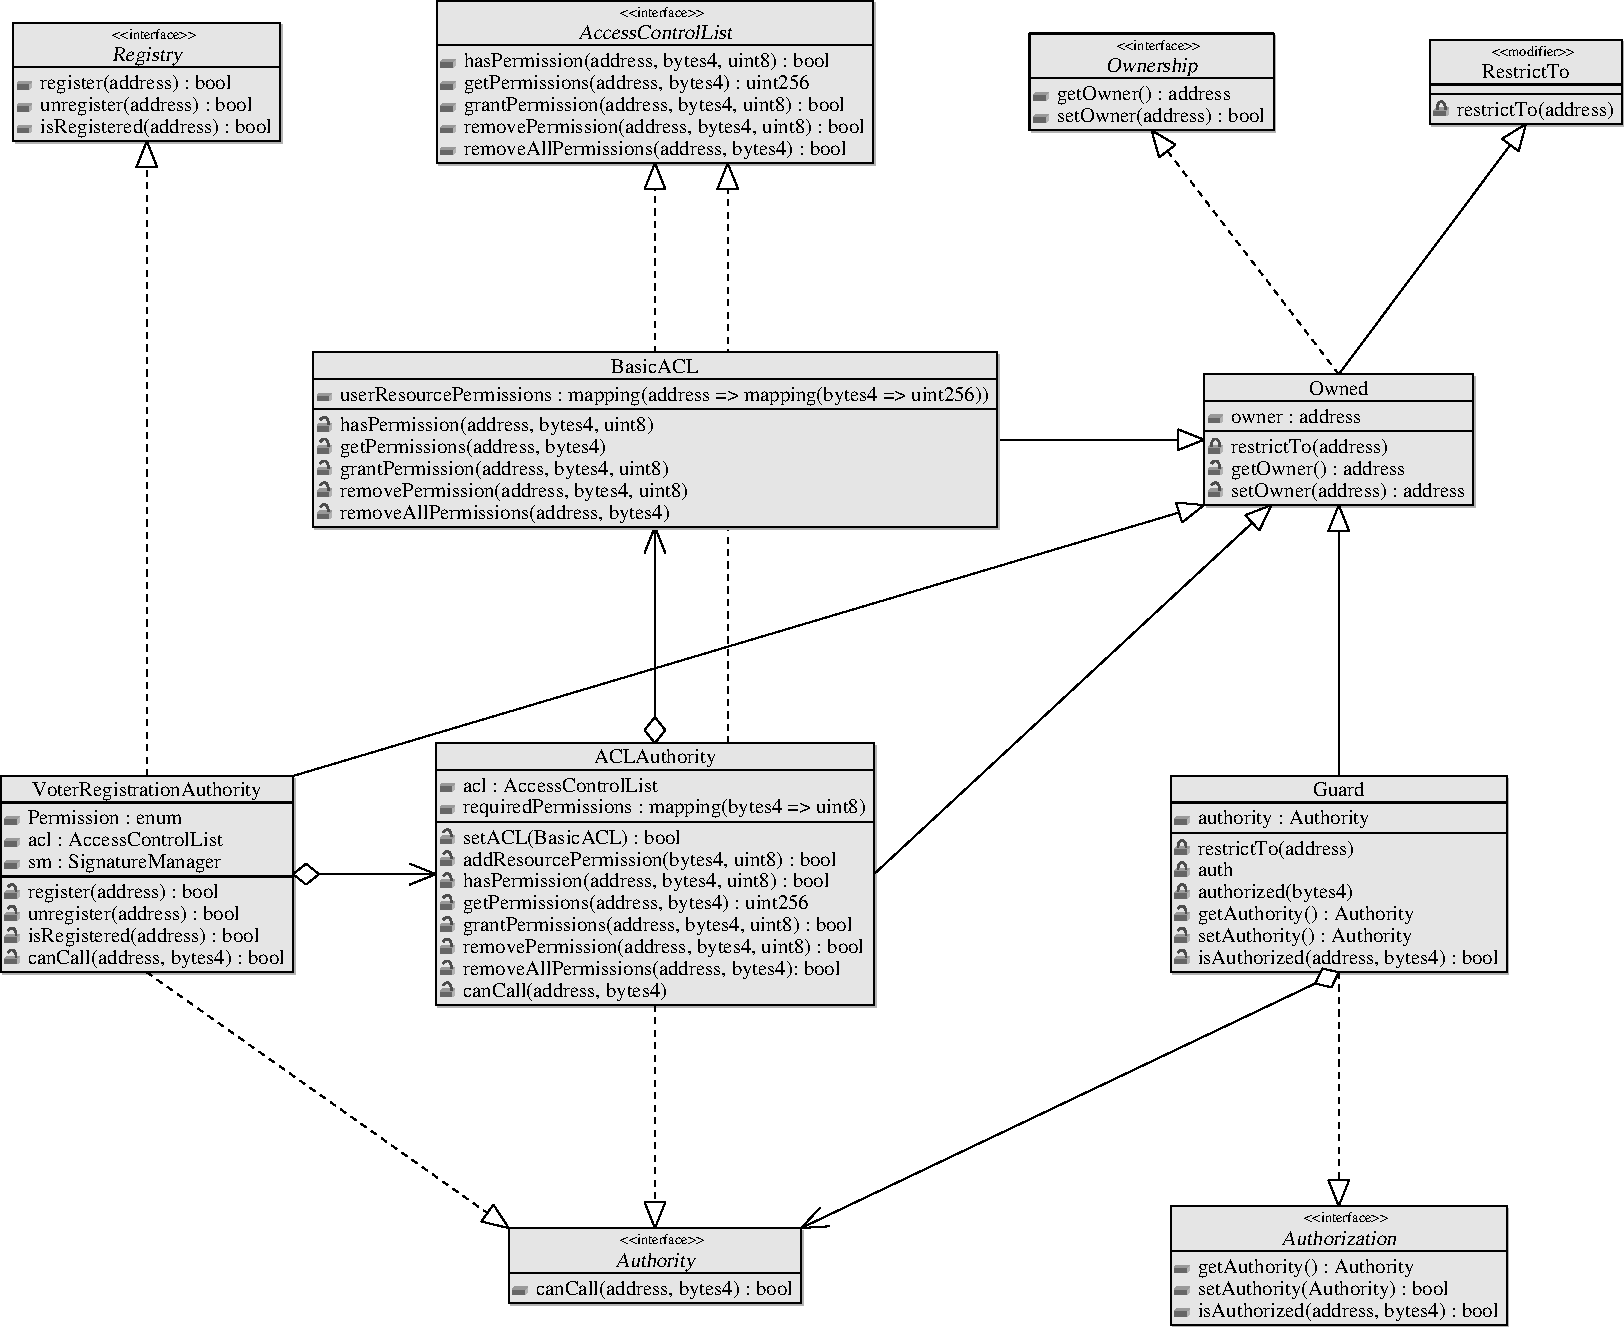
\includegraphics[width=\textwidth]{figures/authorization/figure}
    % \includestandalone[width=\textwidth]{\fig{authorization}}
    \caption{DVBM System Architecture~\cite{dc-voting-system}}\label{fig:dvbm-architecture}% \label{fig:authorization}
\end{figure}

Prior to the official launch of the system the BOEE opted to conduct a mock
election where members of the public, researchers, and hackers alike were
invited to to test the functionality of the system, discover vulnerabilities,
and attempt to compromise the security, reliability, and availability of the
system.\cite{internet-voting-survey,dc-voting-system,trust-the-vote-dc-pilot}

% \paragraph{Outcome}
Within 48 hours of the system going live researchers from The University of
Michigan, playing the role of an attacker, demonstrated a number of
vulnerabilities and attacks on on the system and managed to gained near-complete
control of the election server. Their intrusion was not detected for nearly 2
days.\cite{dc-voting-system}
% Prior to its launch election officials held a mock election to test the security
% of the system, inviting researchers and hackers alike to attempt to compromise
% the security, reliability, and availability of the system. A number of attacks
% were demonstrated and researchers were able to:

Demonstrated vulnerabilities included being able to:
\begin{itemize}
  \item penetrate the network of the election software
  \item determine voter's identities
  \item locate unencrypted ballots, thus mapping voter's identities to their
    personal votes
  \item modify ballots
  \item cast fake ballots
  \item modify the election system software itself
\end{itemize}

Once election officials became aware of the attack, the mock election was
suspended, five days ahead of schedule, citing ``usability issues.'' Election
officials later confirmed that they were unable to detect the attack or network
presence using their intrusion detection system. Due to the test results, the
portion of the system which allowed for ballots to be submitted over the
Internet was not used.\cite{dc-voting-system}

\subsubsection{Estonia --- 2005}
Estonia began using Internet voting in 2005\cite{internet-voting-survey}; in the
2015 Estonian parliamentary elections, 30.5\% of all voters voted over the
Internet. Estonia maintains what is likely the most advanced national
identification cards in the world. Estonian IDs are part of a \emph{Public Key
Infrastructure (PKI)} where IDs serve as smart cards which possess two RSA key
pairs: one for signing and one for authentication; these cryptographic functions
are performed directly on the card. The signatures produced by these IDs are
used extensively throughout the country and are considered legally binding.
These cryptographic IDs allow Estonia to provide voter authentication
capabilities that cannot be reproduced in the US.\ Despite the advanced
authentication capabilities that Estonia is able to achieve, researchers in 2014
devised a number of attacks that could be performed on the Estonian voting
system to spoil ballots, damage ballot secrecy, and steal or drop votes. The
researchers also criticized the transparency and operational security of the
system, noting that videos of the administration processes --- provided for
transparency purposes --- recorded administrators entering root passwords,
revealed network credentials which had been posted on a wall, and showed
administrators using USB drives containing personal files to move sensitive
election materials between systems.\cite{estonia}

% \subsection{Shared Weaknesses}\label{section:shared-weaknesses}
% There are a number of shared weaknesses and vulnerabilities exposed across these
% internet voting systems which the systems incur due to the underlying
% architecture of the systems, their Internet, the personal computer, and remote
% voting.
%
% \begin{enumerate}
%   \item Lack of voter-verified audit trails.
%   \item Vulnerabilities to insider attacks.
%   \item Privacy.
%   \item Vote Buying/Selling.
%   \item Intimidation.
%   \item Large-Scale Impact.
%   \item Too Many Potential Attacks.
%   \item Many Sources of Attacks.
%   \item Undetectable Attacks.
%   \item On-screen Electioneering.
% \end{enumerate}

% \todo{
%   Should I add a shared weaknesses section here and remove some of the
%   demonstrated attacks from the individual systems?
% }


% Section: End-to-End Verifiability
\section{End-to-End Verifiability}\label{sec:e2e-viv}
The vulnerabilities and weaknesses of electronic voting systems demonstrate a
clear need for a stronger kind of system design. \emph{End-to-End Verifiable
(E2E-V)} voting systems are systems which aim to provide such a design by
providing the following features for voters:

\begin{enumerate}
  \item allows voters to check that the system recorded their votes correctly

  \item allows voters to check that the system included their votes in the final
    tally

  \item allows voters to count the recorded votes and double-check the announced
    outcome of the election.
\end{enumerate}

% E2E-V voting systems have been a hotbed of research over the past several years.
An \emph{End-to-End Verifiable Internet Voting (E2E-VIV)} is an E2E-V voting
system that supports voting over the Internet.

% \begin{displayquote}
%    Aggressive early adoption of election technology must be tempered by a clear
%    understanding that voters’ trust in their elections is hard-won and easily
%    lost.
% \end{displayquote}


\subsection{Requirements}
In 2015, the U.S. Vote Foundation published a specification and feasibility
assessment study which laid out requirements for building an end-to-end
verifiable internet voting system. The study broke these requirements into two
categories:\cite{e2e-viv}

\begin{itemize}
  \item \emph{Technical Requirements}, the set of requirements which can be
    directly addressed by system design and architecture

  \item \emph{Non-Functional Requirements}, the set of requirements which must
    be imposed on a system by external entities
\end{itemize}

% cite: The Future of Voting: E2E-VIV
% This section reviews those requirements.

\subsubsection{Technical Requirements}
The ten categories of technical requirements, those which should be addressed
by the design and architecture of the systems itself, are:\cite{e2e-viv}

\begin{enumerate}
    \item functional requirements
    \item accessibility requirements
    \item usability requirements
    \item security requirements
    \item authentication requirements
    \item auditing requirements
    \item system operational requirements
    \item reliability requirements
    \item interoperability requirements
    \item certification requirements
\end{enumerate}

% \paragraph{Functional}
% \begin{displayquote}
%   The functional requirements of an E2E-VIV system deal primarily with the
%   casting and recording of ballots and associated voter records.
% \end{displayquote}

The \emph{functional requirements} deal primarily with casting and recording of
ballots. \emph{Receipt freedom} is one such functional requirement. An
electoral system which expresses receipt freedom is said to make it impossible
for a voter to prove to anyone how they voted.
%
% \subparagraph{Receipt freedom} is one such functional requirement, a property
% where it is impossible for a voter to prove to anybody how they voted.
%
Others functional requirements include:
\begin{itemize}
    \item ensuring that a voter cast a ballot if such an act is recorded
    \item data retention in case of failure
    \item multi-vote functionality to overwrite previous votes
    \item maintaining voter anonymity
\end{itemize}

% \paragraph{Usability}
% \begin{displayquote}
%   The usability of an E2E-VIV system is critical to its successful adoption and
%   use.
% \end{displayquote}

\emph{Usability} is mostly concerned with user experience and confirmation
guarantees. For example, voters should be confident that their vote was cast by
being provided a confirmation screen. The voting process should be both
intuitive and guide the voter through the process. Presentations such as the
butterfly ballot should be avoided at all costs.

% \paragraph{Accessibility}
% \blockquote{\emph{Accessibility} is the property of being usable by and
% useful to voters with disabilities.}

Digital voting systems have the potential to provide wider \emph{accessibility}
guarantees than traditional paper ballots for voters with disabilities. To
provide these guarantees developers must involve voters throughout the
development process to identify accessibility issues and implement solutions.

% \paragraph{Security}
\emph{Security} is an integral property and requirement which voting systems
must maintain. Included in this requirement is that:

\begin{itemize}
    \item no data can be permanently lost
    \item integrity of voters, candidates, ballot information, cast ballots, and
      other critical information must be maintained
    \item accurate timing information is critical for auditing
    \item voting equipment must be protected
    \item the system must perform regular health checks
\end{itemize}

% \paragraph{Authentication}
\emph{Authentication} is the process of ascertaining the validity of a claimed
identity. Authentication ensures that the voting system can enforce privacy and
prevent multi-voting, Sybil attacks, and vote theft. All individuals must be
identified uniquely. The system must allow access to services only to authorized
users, e.g., only allow election officials to load ballot info.

% \paragraph{Auditing}
The property of \emph{auditability} means that a voting system is capable of
comprehensive examination. Auditability must exist at all stages and levels of
the voting process. The system must keep auditable logs of all relevant activity
and the logs must be public and write only. Furthermore, the logs cannot leak
any data regarding voters or the way any ballot was cast. Privacy must always
be the foremost concern.

The auditing system must actively report issues and information in
real-time. At least the following events should be recorded:\cite{e2e-viv}
\begin{itemize}
  \item ``all voting-related information, including the number of eligible
    voters and votes cast, the number of invalid votes, count and recount
    results, etc.''
  \item ``any detected attacks on the operation of the system or its
    communication infrastructure''
  \item ``any system failures, malfunctions, or other detected threats to proper
    system operation.''
\end{itemize}
%
% \blockquote[{\cite[67]{}}]{%
%     \begin{itemize}
%         \item all voting-related information, including the number of eligible voters and
%             votes cast, the number of invalid votes, count and recount results, etc.;
%         \item any detected attacks on the operation of the system or its communication
%             infrastructure; and
%         \item any system failures, malfunctions, or other detected threats to proper
%             system operation.
%     \end{itemize}
% }
%
The system should provide auditing features which support the ability to:\cite{e2e-viv}
\begin{itemize}
  \item ``cross-check and verify the correct operation of the voting system and
    the accuracy of the election results''
  \item ``detect voter fraud''
  \item ``prove that all counted votes are legitimate and that all ballots have
    been counted''
\end{itemize}
%
% \blockquote[{\cite[67]{}}]{%
%     \begin{itemize}
%         \item cross-check and verify the correct operation of the voting system and the
%             accuracy of the election results;
%         \item detect voter fraud; and
%         \item prove that all counted votes are legitimate and that all ballots have been
%             counted.
%     \end{itemize}
% }
%
Finally, auditability must extend to the source code, actions performed, and the
documentation itself.

% \paragraph{System Operational}
\emph{System operational} requirements are those that enforce and regulate
transparency, accountability, system configuration, and updates. Logs, software,
configurations, versions, updates, etc., must all be managed and produced to
audit for tampering. Protocols should be in place to guard sensitive equipment
at all times and handle system failures. Officials managing these systems and
the procedures themselves must be scrutinized closely to prevent insider attacks
and election fraud.

% \paragraph{Reliability}
\emph{Reliability} is the property of a system behaving reasonably and as
expected under both normal conditions and while under attack. During an election
period a system should be highly available. 99.9\% availability is a minimum for
voting systems. The system must also be able to recover from any failure within
10 minutes, with the exception for failure caused by natural disaster or
malicious attack. The system should have redundant backup systems for critical
components of the system.

Internet voting systems are compelling targets for Distributed Denial of Service
(DDoS) attacks, therefore it is important that an E2E-VIV system be hardened to
such attacks and be able to continue operation with full correctness during a
sustained DDoS attack.

% \paragraph{Interoperability}
An E2E-VIV system must use open standards for \emph{interoperability} between
components, services, and other E2E-VIV systems. Logs and documentation of such
standards must be published so that anyone can download, inspect, and publish
analysis and concerns.

% \paragraph{Certification}
Finally, there should be \emph{certification} and test procedures involved for
every functional requirement; these tests should be able to be run on demand.
Formal proofs of security and correctness should be provided wherever possible,
and third-parties should be hired to conduct an independent review, audit, and
test of the system.

\subsubsection{Non-functional Requirements}
The five non-functional requirements defined, those which must be fulfilled by
external entities, e.g., operators and administrators, are:\cite{e2e-viv}

\begin{enumerate}
    \item operational requirements
    \item procedural requirements
    \item legal requirements
    \item assurance requirements
    \item maintenance/evolvability requirements
\end{enumerate}

% \paragraph{Operational}
The specification describes several \emph{operational} requirements: election
and registration timing, maintaining voter registration and candidate
nomination lists, providing receipt freedom, voter assistance, election
integrity, and openness.

% \subparagraph{Voter Assistance}
Voters must be well-informed on how to register, vote, and protect their privacy
in the voting system.
% \subparagraph{Election and Registration Timing}
Clear instruction on when voting and registration occurs should be announced far
in advance for the voter's benefit. When multiple forms of remote voting take
place, votes cast over the Internet should not be accepted after other forms of
remote voting end.
% \subparagraph{Voter Registration}
E2E-VIV systems must publish a voter register that is regularly updated. Voters
should be able to check that information in the register is accurate and request
corrections.
% \subparagraph{Candidate Nomination Lists}
The ballot presented to voters must be consistent, fair, unbiased, and free from
any superfluous information about candidates/choices.

% \subparagraph{Receipt Freedom}
Operational receipt freedom represents two different requirements depending on
whether a voter is voting from a supervised or unsupervised location. In a
supervised location receipt freedom requires that the voting terminal clear all
indication of how a ballot was cast and ensure that no paper trail representing
how the ballot was cast is able to leave the polling place (except by official
means). In an unsupervised location any visual proof of vote should not be able
to be used to determine how a vote was cast or will be tallied.

% \subparagraph{Election Integrity}
If test ballots are capable of being submitted then those ballots must be
clearly marked as a test ballot with instruction on how to cast a real ballot.
The voting system should not disclose any results to any person until after the
voting period has ended, including alternative forms of voting. Tallying should
be done as soon as possible afterwards and the tallying process should be
transparent, recorded, and be able to be replayed. Any irregularities which
affect the integrity of votes should be recorded.

% \subparagraph{Openness}
An E2E-VIV system must be open and function properly regardless of the hardware
or software being used to run the voting software. The system must be available
for auditing by external actors, especially when considering components which
are expected to be run on external systems or voter's machines.

% \paragraph{Procedural}
\emph{Procedural} requirements define the processes required to deploy and run
the E2E-VIV system.

\begin{itemize}
  \item Procedures should be published regarding provisioning, certification,
    maintenance, availability, and use. For example, when updates occur,
    election officials must call upon an independent body to perform
    verifications of performance and certification of intent.

  \item Procedures should be in place to teach voters the voting process.

  \item Election officials should have maintenance and security procedures to
    ensure that voting equipment is operating nominally and has not been
    tampered with. For example, conducting sensitive operations should require
    teams of at least two people.

  \item As much as possible there should be procedures in place to allow
    observers to watch election procedures.

  \item Procedures should be in place to update results in the event that a
    voter proves that their vote was not accurately received or counted.
\end{itemize}

% \paragraph{Legal}
The \emph{legal} requirements include national, state, and local laws that apply
to voting systems, e.g., accessibility, anonymity, and availability guarantees.
Any deployed E2E-VIV system must comply with these laws. For example, election
officials must ensure that only one ballot by each voter is tallied when
multiple means of voting exist, e.g., remote and traditional polling place.
%
% Voters must be able to restart, discard, or alter their votes at any point
% during the voting process. The system must allow the voter to participate in an
% election without marking choices, i.e., casting blank or partially blank
% ballots. The voting system must always preserve anonymity and indicate clearly
% that the voters ballot has been cast and voting procedure completed.
%
\begin{displayquote}
  ``There must be no impediments to interested parties who want to study the
  E2E-VIV system. In particular, no nondisclosure agreement or contract of any
  kind may be required for download and study of, or for building, testing and
  publishing test results for, the E2E-VIV system.''\cite{e2e-viv}
\end{displayquote}
% \blockquote{There must be no impediments to interested parties who want to study
% the E2E-VIV system. In particular, no nondisclosure agreement or contract of any
% kind may be required for download and study of, or for building, testing and
% publishing test results for, the E2E-VIV system.}

% \paragraph{Assurance}
To meet \emph{assurance} requirements, client-side software must be functional
and free of bugs across a wide range of hardware and software stack
combinations. There must be strong security with respect to authentication such
that voter credentials cannot be forged or invalidated without breaking
underlying cryptographic protocols.

The entirety of the voting system --- e.g., software, documentation, design,
architecture, algorithms, build scripts, issue tracking system, etc. --- must be
free, open, and public. All available resources should be up to date, certified,
and released under license that permits anyone to download, build, test, or
modify the source.

% \paragraph{Maintenance and Evolvability}
To meet \emph{maintenance and evolvability requirements} election officials must
have the right and ability to update the election system to conform to law,
technology, or threat independent of the original vendor.

\subsection{Architecture}
% \todo{Improve the Architecture content.}
The study, ``The Future of Voting: End-to-End Verifiable Internet Voting,''
provides an architectural feature model, seen in Figure~\ref{fig:viv-model},
which defines over 127,000 possible architectural variants.\cite{e2e-viv}

\begin{figure}[H]
  \setstretch{1}
  \begin{Verbatim}[
    label={[Architectural Feature Model]Architectural Feature Model},
    tabsize=2,
    fontsize=\scriptsize,
    frame=lines,
    framesep=5mm,
    numbers=left,
    fillcolor=\color{yellow}
  ]
  -- This diagram shows the various dimensions of an E2EVIV architecture
  static_diagram E2EVIV_Architecture_Dimensions
  component
    class E2EVIV_ARCHITECTURE
    feature
      authority_distribution: SET[VALUE]
        ensure 0 < Result.count;
          for_all v: VALUE such_that v member_of Result
            it_holds v member_of { Centralized, Distributed };
        end
      crypto_protocols: SET[VALUE]
        ensure 0 < Result.count;
          for_all v: VALUE such_that v member_of Result
            it_holds v member_of { On_Paper, Mechanized, Verified, Generated };
        end
      correctness_evidence: SET[VALUE]
        ensure 0 < Result.count;
          for_all v: VALUE such_that v member_of Result
          it_holds v member_of { Process_Based, Assertions };
        end
      implementation_type: SET[VALUE]
        ensure 0 < Result.count;
          for_all v: VALUE such_that v member_of Result
            it_holds v member_of { Golden_Implementation, Open_Protocols_and_Specs };
        end
      key_distribution_method: SET[VALUE]
        ensure 0 < Result.count;
          for_all v: VALUE such_that v member_of Result
            it_holds v member_of { Public_Ceremony, Threshold_Cryptography, PKI, Web_of_Trust };
        end
      deployment_style: SET[VALUE]
        ensure 0 < Result.count;
          for_all v: VALUE such_that v member_of Result
            it_holds v member_of { Trusted_Servers, Public_Cloud, Peer_to_Peer };
        end
      client_technology: SET[VALUE]
        ensure 0 < Result.count;
          for_all v: VALUE such_that v member_of Result
            it_holds v member_of { Custom_App, Web_Based };
        end
    end
  end
  \end{Verbatim}
  \caption{A specification of the possible variants for an E2E-VIV system.\cite{e2e-viv}}\label{fig:viv-model}
\end{figure}

Most of the variability available when constructing an E2E-VIV system stems from
the cryptographic techniques and tools available to select from when designing
the system.

\subsubsection{Cryptographic Techniques and Tools}
The cryptographic techniques and cryptosystems available for use in E2E-V
electoral systems are presented in this section; this is not a comprehensive
list of cryptographic techniques and tools available, but includes some of the
most common techniques and tools leveraged in E2E-VIV systems.

% \paragraph{Asymmetric Cryptography}
Asymmetric cryptography, also known as public-key cryptography, uses pairs of
keys to securely encrypt and decrypt messages. There are many different
public-key based cryptosystems available for use.

% \paragraph{Homomorphic Schemes}
Homomorphic cryptographic schemes allow one to perform basic arithmetic
operations on ciphertexts without requiring decryption of the ciphertext. This
property has a number of uses in E2E-VIV systems; for example, an E2E-VIV system
might leverage this property to tally a collection of encrypted ballots without
decrypting any individual's ballots.

% \subparagraph{Additive Homomorphic Encryption}
Additive homomorphic encryption schemes enable processing of ciphertexts by way
of addition. The Pallier and Benaloh cryptosystems both support additive
homomorphic encryption.\cite{helios}

% \subparagraph{Multiplicative Homomorphic Encryption}
Multiplicative homomorphic encryption schemes enable processing ciphertexts by
way of multiplication. The ElGamal cryptosystem supports multiplicative
homomorphic encryption.

% \paragraph{Append-Only Public Bulletin Board}
Most E2E-VIV systems depend on an append-only web/public bulletin
board.\cite{bulletin-board} The append-only public bulletin board is a
publicly-visible secure location where election operations and ballot data are
submitted, logged, and made available to support auditing
requirements.\cite{e2e-viv,helios,almost-correct-mixing,pretty-good-democracy,mix-networks,vector-ballot-voting}
Blockchains fulfill most of the requirements of an append-only public bulletin
board.

% \subsubsection{Secret Sharing and Threshold Schemes}
Secret sharing and threshold schemes allow a collection of actors to cooperate
to produce ``shares'' of a secret; each participant is responsible for
managing their share of the secret and some threshold of shares must come
together to recover the complete secret or perform cryptographic
operations.\cite{distributed-key-generation,large-scale-distributed-key-generation}

% \paragraph{Zero-Knowledge Proofs}
A zero-knowledge proof (ZKP) is a probabilistic method which allows one party
to prove knowledge of some secret without revealing any information about the
secret itself. A zero-knowledge proof satisfies the following properties:\cite{e2e-viv,zkproof}
%
\begin{enumerate}
  \item Completeness, an honest verifier will be convinced by an honest prover.
  \item Soundness, an honest verifier will not be convinced by a dishonest
    prover.
  \item Zero-knowledge, the verifier will not learn any information regarding
    the secret itself.
\end{enumerate}
%
% \subparagraph{Non-Interactive Zero-Knowledge Proofs}
A useful form of zero-knowledge proofs are non-interactive zero-knowledge
proofs --- also known as NIZKs, zk-SNARKs, or zkSTARKs --- which are
zero-knowledge proofs which require no interaction between the prover and
verifier for the verifier to be convinced of
correctness.\cite{helios,almost-correct-mixing,vector-ballot-voting,mix-networks}

% \paragraph{Mixnet Schemes}
Mixnet schemes are used to provide anonymity. Mix networks are operated by a
set of trusted nodes, mix-servers, which consume messages --- typically
encrypted ballot data in the case of E2E-VIV systems --- from a set of
network-participants to produce a random permutation of the input messages.
Each node performs a ``mix'' operation on the incoming messages in such a way
that the output cannot be unscrambled and tied back to a network-participant
except by the node itself which is performing the mixing operation. Therefore,
as long as any single mix-server in the mix network is acting honestly, the
anonymity of the participants will be
maintained.\cite{mix-networks,vector-ballot-voting}

% \subparagraph{Decryption Mixnet}
A decryption mixnet operates by encrypting a message in multiple layers with
each mix server's public key. To decrypt the message, the message layers are
decrypted in the opposite order they were encrypted in by each node. Each node
forwards its decrypted results to the next node in the mix network. So long as a
single node does not reveal the source of the message then the message will
become untraceable (assuming no information is leaked by the message
itself).\cite{mix-networks}

% \subparagraph{Re-encryption Mixnet}
A re-encryption mixnet works by leveraging the re-encryption properties of the
underlying encryption scheme. Certain cryptosystems make it possible to change a
ciphertext without modifying the underlying message. In this way a set of nodes
can shuffle and re-encrypt a ciphertext then pass them to the next mixnet node
to repeat the process. So long as a single node does not reveal the shuffling
process the anonymity offered by the mixnet will be
maintained.\cite{mix-networks,almost-correct-mixing}

% \paragraph{Blind Signature Schemes}
Blind signature schemes separate the voter authentication, authorization, and
signing components from the vote tallying, shuffling, and decryption components.
A voter will encrypt a ballot (blind it) then send it to a signing authority who
will blind-sign the encrypted ballot after it has verified that the voter is
qualified to vote. Once a voter has acquired a blind signed ballot they can
strip their identifying data, unblind the ballot, and submit the signed ballot
through an anonymous channel. The underlying cryptosystem makes it such that the
blind signed ballot is equivalent to a signed unblinded ballot.\cite{e2e-viv}

% cite

% \paragraph{ElGamal}
% The ElGamal cryptosystem is a
%
% \paragraph{Paillier}

% \subsection{Existing Systems}
% \todo{Complete section.}
% \todo{Do not directly discuss any systems which are strictly physical.}

% \subsubsection{Estonia}
% Estonia began using Internet voting in 2005. By the 2015 Estonian parliamentary
% elections 30.5\% of all voters voted over the Internet. Estonia maintains what
% are probably the most advanced national identification cards in the world.
% Estonian IDs are part of a \emph{Public Key Infrastructure (PKI)} where IDs
% serve as smart cards which possess two RSA key pairs: one for signing and one
% for authentication. Cryptographic functions are performed on the card. The
% signatures produced by the IDs are used extensively throughout the country and
% are legally binding. These cryptographic IDs allow Estonia to provide voter
% authentication capabilities that cannot be reproduced in the US.\ Despite the
% advanced authentication capabilities that Estonia offers researchers in 2014
% devised a number of attacks that could be performed on the Estonian voting
% system to spoil ballots, damage ballot secrecy, and steal/drop votes. The
% researchers also criticized the transparency and operational security of the
% system.

% \subsubsection{Helios}
% \todo{Review Ben Adidas' Helios system.}

% \subsubsection{RIES}
% \todo{Complete section.}

% \subsubsection{Pret A Voter}
% \todo{Special characters/spelling in pret a voter.}

% \subsubsection{Punchscan}
% \todo{Complete section.}
%
% \subsubsection{Scantegrity II}
% \todo{Complete section.}

% \subsubsection{Remotegrity}
% \todo{Complete section.}

% \subsubsection{Norwegian System}
% \todo{Complete section.}

% \subsubsection{Wombat}
% \todo{Review Wombat.}
% \todo{Complete section.}

% \subsubsection{Demos}
% \todo{Complete section.}
% \todo{Review Demos.}

% \subsubsection{vVote}
% \todo{Complete section.}


% Section: Notable Voting Systems and Experiments
% % \section{Novel Electoral Systems, Voting Experiments, and Technologies}
\section{Notable Voting Systems \& Experiments}
What follows is a review of other notable voting systems and experiments:

\subsection{Novel Voting Systems}

\subsubsection{Estonia}
Estonia began using Internet voting in 2005. By the 2015 Estonian parliamentary
elections 30.5\% of all voters voted over the Internet. Estonia maintains what
are probably the most advanced national identification cards in the world.
Estonian IDs are part of a \emph{Public Key Infrastructure (PKI)} where IDs
serve as smart cards which possess two RSA key pairs: one for signing and one
for authentication. Cryptographic functions are performed on the card. The
signatures produced by the IDs are used extensively throughout the country and
are legally binding. These cryptographic IDs allow Estonia to provide voter
authentication capabilities that cannot be reproduced in the US.\ Despite the
advanced authentication capabilities that Estonia offers researchers in 2014
devised a number of attacks that could be performed on the Estonian voting
system to spoil ballots, damage ballot secrecy, and steal/drop votes. The
researchers also criticized the transparency and operational security of the
system.

\subsection{Blockchain Voting Systems}
\todo{Compare and contrast other electoral systems with this research, discuss
weaknesses, holes in the research, etc.}

% \subsection{Voting Machines}
% \todo{Complete section.}
%
% % #### Diebold AccuVote-TS
% \subsubsection{Diebold AccuVote-TS}
% \todo{Complete section.}
%
% % #### AVS WINVote
% \subsubsection{AVS WINVote}
% \todo{Complete section.}

% \subsection{Voting Experiments}

% ### Demonstrated Attacks
% The following is a review of Internet voting systems that research has shown to
% be susceptible to attack.


% \subsection{Voting Technologies}

% ### Demonstrated Attacks
% The following is a review of electronic voting machines that research has
% shown to be susceptible to attack.
%
% \subsection{Compare and Contrast}

% \todo{Add back the Novel Electoral Systems section once it has been improved.}

% Section: Ethereum
% \subsection{Ethereum}

Ethereum is a blockchain-based system initially proposed in late 2013,
post-Bitcoin, and released in 2015.\cite{ethereum-white} Ethereum introduced a
few novel features and functionalities with its blockchain network which are not
available in the Bitcoin network. Most notably Ethereum offers a distributed
decentralized Turing-complete computing platform via the Ethereum Virtual
Machine (EVM), which aims to provide an application layer which ``[runs] exactly
as programmed without any possibility of downtime, censorship, fraud or third
party interference.''\cite{ethereum.org,ethereum-yellow}

\subsubsection{Fundamental Concepts}

\paragraph{Currency}
Like Bitcoin, Ethereum's blockchain defines and leverages its own token,
\solt{ether} --- also referred to as \solt{eth} or ETH, and sometimes denoted
using the Greek symbol Xi, $\Xi$, the uppercase Old English letter Eth, \DH, or,
more rarely, $\blacklozenge$ --- which acts as the underlying currency of its
blockchain protocol. The smallest unit of \solt{ether} is
\emph{wei}.~\cite{mastering-ethereum,ethereum-yellow} The
denominations of \solt{ether} are broken down as follows:
% \ref{book:mastering-ethereum}
% \ref{paper:ethereum}

% \todo{Add denomination table here}

% \ref{book:mastering-ethereum}
% \ref{paper:ethereum}
%
% See page 2 of Ethereum yellow paper.
%
% Table 2-1 from page 14 of Mastering Ethereum.
%
% | Value (in wei) | Exponent | Common Name | SI Name               |
% |----------------|----------|-------------|-----------------------|
% | 1              | 1        | wei         | Wei                   |
% | 1000           | 10^3     | Babbage     | Kilowei or femroether |
% |                |          |             |                       |
% |                |          |             |                       |

\begin{center}
    \setstretch{1.5}
    \footnotesize
    \begin{longtabu} to \textwidth{@{} X[3] X[] X[] X[2] @{}}
    \caption{Ether Denominations~\cite{mastering-ethereum}}\label{tab:eth-denominations} \\
    \toprule
    Value (in wei)                    & Exponent & Common Name & SI Name \\
    \midrule
    \endfirsthead
    \toprule
    Value (in wei)                    & Exponent & Common Name & SI Name \\
    \midrule
    \endhead
    \taburowcolors{white..gray!15}
    1                                 & $10^{0}$    & wei       & Wei \\
    1,000                             & $10^{3}$    & Babbage   & Kilowei or femtoether \\
    1,000,000                         & $10^{6}$    & Lovelace  & Megawei or picoether \\
    1,000,000,000                     & $10^{9}$    & Shannon   & Gigawei or nanoether \\
    1,000,000,000,000                 & $10^{12}$   & Szabo     & Microether or micro \\
    1,000,000,000,000,000             & $10^{15}$   & Finney    & Milliether or milli \\
    1,000,000,000,000,000,000         & $10^{18}$   & Ether     & Ether \\
    1,000,000,000,000,000,000,000     & $10^{21}$   & Grand     & Kiloether \\
    1,000,000,000,000,000,000,000,000 & $10^{24}$   &           & Megaether \\

    %extern u256 const c_copyGas;			///< Multiplied by the number of 32-byte words that are copied (round up) for any *COPY operation and added.
    \bottomrule
    % \begin{varwidth}{\textwidth}
    %   These names pay homage to some of the great minds of cryptography and
    %   computer science.
    % \end{varwidth}
  \end{longtabu}
\end{center}

\paragraph{Accounts}
Accounts are an Ethereum primitive which provide an abstraction over the Bitcoin
equivalent signature chain process; this abstraction helps to both simplify the
concept of token ownership as well as extend the idea of what a token is, what a
token can be, and how blockchain state can be managed and organized.

Accounts are identified by a 160-bit code, their \solt{address}, and are
internally represented by four properties:

\begin{enumerate}
  \item \sol{nonce}, a monotonically increasing counter which represents the
    number of transactions sent from the account.
  \item \sol{balance}, the amount of \solt{ether}, expressed in wei, which is
    owned by the account.
  \item \sol{storageRoot}, a 256-bit hash of the root node of a Merkle Patricia
    tree which encodes the storage contents of the account.

    % RLP - Recursive Length Prefix
    % https://eth.wiki/en/fundamentals/rlp

    % https://blog.ethereum.org/2015/11/15/merkling-in-ethereum/
    %
    % From the yellow paper:
    % \displayquote{
    %   A 256-bit hash of the root node of a Merkle Patricia tree that encodes
    %   the storage contents of the account (a mapping between 256-bit integer
    %   values), encoded into the trie as a mapping from the Keccak 256-bit hash
    %   of the 256-bit integer keys to the RLP-encoded 256-bit integer values.
    %   This tree encodes the hash of the storage contents of this account, and
    %   is empty by default.
    % }


  \item \sol{codeHash}, an immutable hash of the EVM code corresponding to the
    account.
\end{enumerate}

Although all accounts are structurally identical it is useful to distinguish
between the two practical kinds of accounts which one is likely to encounter and
interact with on the Ethereum blockchain, \emph{external accounts} and
\emph{internal accounts}:
%
\begin{description}[font=\normalfont\emph]
  % \subsubparagraph{External Accounts}
  \item[External Accounts] --- also referred to as simple accounts, non-contract
    accounts, externally owned accounts (EOA), and sometimes user accounts ---
    are defined as accounts whose \sol{codeHash} value is the Keccak-256 hash of
    an empty string; i.e., the account contains no code.

  %\subsubparagraph{Internal Accounts}
  \item[Internal Accounts] --- also referred to as contract accounts --- are
    those accounts which are not external accounts; i.e., the account contains
    code.
\end{description}
%
Both kinds of accounts have the ability to send and receive \solt{ether} as well
as interact with \solt{contract}[s] which have been deployed to the Ethereum
network. However, there are some key differences between the two kinds of
accounts which are worth highlighting:\cite{ethereum:accounts}

\begin{itemize}[label=]
  \item External Accounts
    \begin{itemize}[label=$\bullet$]
      \item External accounts are managed by public-key cryptography.
      \item External account creation costs no \solt{ether}.
      \item Only external accounts can \emph{initiate} transactions.
      \item Transactions between external accounts can only transact
        \solt{ether}.
    \end{itemize}
  \item Internal Accounts
    \begin{itemize}[label=$\bullet$]
      \item Internal accounts are managed by code.
      \item Internal account creation costs \solt{ether} which reflects the cost
        of storing code on the Ethereum network.
      \item Internal accounts can execute code via the EVM upon receiving
        transactions, enabling a wide range network functionalities.
      \item Internal accounts can only send transactions in response to
        receiving transactions. \todo{This will have a major impact on the
        methodologies.}
    \end{itemize}
\end{itemize}

\paragraph{Transactions}
A transaction is a cryptographically-signed instruction constructed by an
external actor and submitted to the Ethereum network. There are two kinds of
transactions worth distinguishing, contract creation transactions and message
call transactions; both kinds of transactions share the following common
properties:

\begin{enumerate}
  \item \sol{to}, a 160-bit \solt{address} representing the \emph{recipient's}
    account. This value is omitted when building a contract creation
    transaction.

  \item \sol{from}, a signature which identifies the \emph{sender} of the
    transaction by account \solt{address}.\footnotemark{}

    \footnotetext{
      This field does not \emph{technically} exist, in actuality the signature
      is represented as three distinct fields (\emph{v}, \emph{r}, \emph{s}),
      which can be used to determine the \solt{address} representing the sender
      of the transaction.
    }

  \item \sol{value}, the amount of \solt{ether}, expressed in wei, which is
    to be transferred to the recipient.

  \item \sol{nonce}, a value equal to the number of transactions which have been
    sent by the \emph{sender}.

  \item \sol{gasPrice}, a value representing the amount of wei to be paid per
    unit of gas (expanded on below).

  \item \sol{gasLimit}, a value representing the maximum amount of gas which
    should be used executing the transaction.
\end{enumerate}

Contract creation transactions include the following additional property in the
transaction:

\begin{enumerate}
  \item \sol{init}, an EVM-code fragment which is executed only once and
    discarded thereafter; it returns the \sol{body}, a second fragment of code
    that executes each time the account receives a message call, which can occur
    either by transaction or internal execution of code.
\end{enumerate}

In contrast, a message call transaction includes the following additional
property:

\begin{enumerate}
  \item \sol{data}, an unlimited size byte array which contains the input data
    of the message call.
\end{enumerate}

\paragraph{Ethereum Virtual Machine}\label{eth:evm}
The Ethereum Virtual Machine (EVM) is the execution environment which Ethereum
code is processed in. The EVM processes low-level bytecode and takes actions
against the state of the Ethereum blockchain in response: reading, processing,
and writing data. The Ethereum Virtual Machine Specification introduces a
low-level instruction set which defines the available operations which an EVM
implementation should support: the opcodes, their inputs, outputs, and various
other implementation details. The EVM can be described as a \emph{state
transition function}, $Y(S, T) = S'$; given a set of transactions, $T$, and an
initial state, $S$, the state transition function, $Y(S, T)$, will produce a new
output state, $S'$.\cite{ethereum-yellow} Several EVM implementations exist
which have been written in various languages, e.g., Go, Python, and C++.

\subparagraph{Language Support}\label{eth:languages}
Several higher-level languages exist which target the Ethereum Virtual Machine
and can be used to build ``smart contracts;'' e.g., Solidity which draws
inspiration from C++ and JavaScript, and Vyper which describes itself as a
``Pythonic Smart Contract Language.'' These languages ship with compilers which
can be used to translate their code into low-level EVM bytecode; Solidity, for
example, is compiled using \solt{solc}, the Solidity compiler.

% \subsubsection{Network Topology}
\subsubsection{Network Topology}
Like Bitcoin, Ethereum exists as a network of nodes, each node supporting
differing functionalities, which work collectively to construct the Ethereum
blockchain and support the surrounding ecosystem. These nodes can be classified
by the functionalities which they support.

\paragraph{Node Types}
There exists several implementations of the Ethereum protocol, i.e., Ethereum
clients, which have been written in various languages, e.g., Geth in Go, Parity
in Rust, and pyethereum in Python. Some of these clients support running in
different modes.

\begin{itemize}
  \item A \emph{full node} is a complete implementation of the Ethereum
    protocol. A full nodes processes and validates all transactions which have
    been added to the Ethereum blockchain, thus helping to support the
    resiliency and reliability of the network. To support this functionality, a
    full node must maintain a complete copy of the blockchain. Full nodes are
    also capable of deploying and interacting with contracts, support mining and
    wallet functionality, and are able to route transactions throughout the
    network.

  \item A \emph{remote client} supports a subset of the functionality that a
    full node supports, generally wallet functionality and the ability to
    broadcast transactions. Other more complex functionalities generally require
    interacting with with a full node or other remote services which are capable
    of fulfilling requests on a remote client's behalf.
\end{itemize}

\paragraph{The Blockchain}
Like Bitcoin, the Ethereum blockchain is constructed by leveraging a
Proof-of-Work (PoW) algorithm to reach consensus throughout the network. The
proof-of-work algorithm leveraged by Ethereum, Ethash, helps to build trust and
reliability throughout the network while also securing the blockchain and
ensuring that EVM code execution has been processed and that the results
produced from said execution are as expected. Ethereum offers cryptoeconomic
incentivization in the form of \solt{ether} to promote participation in the
proof-of-work process.\cite{ethereum-yellow}

\subparagraph{Blocks}
The Ethereum protocol groups collections of transactions into \emph{blocks}.
Blocks are linked to previous blocks, via cryptographic hash, which reflect the
prior states of the blockchain. When processed collectively these blocks reflect
the current state of the Ethereum blockchain.

\subparagraph{Proof-of-Work}
Ethereum's proof-of-work algorithm, Ethash, is a proof-of-work algorithm which
was initially inspired by the Hashimoto and Dagger algorithms. The primary
motivation behind the Ethash algorithm was to produce a PoW algorithm which
would be resistant to application-specific integrated circuits (ASICs). The
primary mechanism leveraged to achieve ASIC-resistance lies in the algorithm's
memory-bound nature: a significant amount of memory, in addition to computation,
is required to correctly compute a proof-of-work solution. By requiring large
amounts of memory-bound operations the algorithm makes itself resistant to most
kinds of specialized memories and caches. Additionally, the memory requirements
are designed to grow and shift over time such that building rapid static caches
would become prohibitively expensive. In some sense the Ethash algorithm might
be better described as Proof-of-Memory.\cite{dagger-hashimoto,hashimoto,dagger}

The Ethereum network has been attempting to migrate away from Ethash to a
lower-cost consensus algorithm operating through Proof-of-Stake (PoS) but has
yet to complete the transition.

% Talk about the Greedy Heaviest Observed Subtree (GHOST) protocol.

\subparagraph{Gas}
In order to validate that EVM code has been executed, and executed as expected,
each full node on the network must recompute all transactions and whatever EVM
code those transactions have triggered when validating blocks. It is not
difficult to imagine how this might cause serious problems and introduce room
for exploitation within the network, \sol{while true { expensiveOperation() }}.
In order to address this the Ethereum specification introduces an abstraction,
\emph{gas}, which has a market-based value and must be paid by the
transaction-sender up-front when generating a transaction. Each operation
computed by the EVM has an associated gas-price and that gas price is ``paid''
to the node who successfully mints a block. If an insufficient amount of gas is
provided by the transaction-sender then the EVM will throw an out-of-gas (OOG)
exception: execution halts, the blockchain state is restored, and all gas
submitted is forfeited to the node. If an excess of gas is provided then any gas
remaining after transaction execution is refunded to the sender. When generating
a transaction on the Ethereum network the creator of the transaction has the
choice of defining how much wei they are willing to pay per unit of gas. Nodes
are incentivized to process transactions which offer more wei per unit of gas
relative to the rest of the transactions available for processing on the
network. Table~\ref{tab:gas-costs} introduces gas costs as defined by the
Ethereum Yellow Paper.


% Stuff about gas. What follows is a table of some gas costs as defined in the Ethereum
% yellow paper.

\begin{center}
  \setstretch{1.5}
  \scriptsize
  \begin{longtabu} to \textwidth{@{} X[1.1,l] X[0.5,r] X[7,l] @{}}
  \caption{Fee Schedule\cite{ethereum-yellow}}\label{tab:gas-costs} \\
  \toprule
  Name & Value & Description* \\
  \midrule
  \endfirsthead
  \toprule
  Name & Value & Description* \\
  \midrule
  \endhead
  \taburowcolors{white..gray!15}
  $G_{zero}$ & 0 & Nothing paid for operations of the set {\tiny $W_{zero}$}. \\
  $G_{base}$ & 2 & Amount of gas to pay for operations of the set {\tiny $W_{base}$}. \\
  $G_{verylow}$ & 3 & Amount of gas to pay for operations of the set {\tiny $W_{verylow}$}. \\
  $G_{low}$ & 5 & Amount of gas to pay for operations of the set {\tiny $W_{low}$}. \\
  $G_{mid}$ & 8 & Amount of gas to pay for operations of the set {\tiny $W_{mid}$}. \\
  $G_{high}$ & 10 & Amount of gas to pay for operations of the set {\tiny $W_{high}$}. \\
  $G_{extcode}$ & 700 & Amount of gas to pay for operations of the set {\tiny $W_{extcode}$}. \\
  $G_{balance}$ & 400 & Amount of gas to pay for a {\tiny BALANCE} operation. \\
  $G_{sload}$ & 200 & Paid for a {\tiny SLOAD} operation. \\
  $G_{jumpdest}$ & 1 & Paid for a {\tiny JUMPDEST} operation. \\
  $G_{sset}$ & 20000 & Paid for an {\tiny SSTORE} operation when the storage value is set to non-zero from zero. \\
  $G_{sreset}$ & 5000 & Paid for an {\tiny SSTORE} operation when the storage value's zeroness remains unchanged or is set to zero. \\
  $R_{sclear}$ & 15000 & Refund given (added into refund counter) when the storage value is set to zero from non-zero. \\
  $R_{selfdestruct}$ & 24000 & Refund given (added into refund counter) for self-destructing an account. \\
  $G_{selfdestruct}$ & 5000 & Amount of gas to pay for a {\tiny SELFDESTRUCT} operation. \\
  $G_{create}$ & 32000 & Paid for a {\tiny CREATE} operation. \\
  $G_{codedeposit}$ & 200 & Paid per byte for a {\tiny CREATE} operation to succeed in placing code into state. \\
  $G_{call}$ & 700 & Paid for a {\tiny CALL} operation. \\
  $G_{callvalue}$ & 9000 & Paid for a non-zero value transfer as part of the {\tiny CALL} operation. \\
  $G_{callstipend}$ & 2300 & A stipend for the called contract subtracted from $G_{callvalue}$ for a non-zero value transfer. \\
  $G_{newaccount}$ & 25000 & Paid for a {\tiny CALL} or {\tiny SELFDESTRUCT} operation which creates an account. \\
  $G_{exp}$ & 10 & Partial payment for an {\tiny EXP} operation. \\
  $G_{expbyte}$ & 50 & Partial payment when multiplied by $\lceil\log_{256}(exponent)\rceil$ for the {\tiny EXP} operation. \\
  $G_{memory}$ & 3 & Paid for every additional word when expanding memory. \\
  $G_\text{txcreate}$ & 32000 & Paid by all contract-creating transactions after the {\it Homestead transition}.\\
  $G_{txdatazero}$ & 4 & Paid for every zero byte of data or code for a transaction. \\
  $G_{txdatanonzero}$ & 68 & Paid for every non-zero byte of data or code for a transaction. \\
  $G_{transaction}$ & 21000 & Paid for every transaction. \\
  $G_{log}$ & 375 & Partial payment for a {\tiny LOG} operation. \\
  $G_{logdata}$ & 8 & Paid for each byte in a {\tiny LOG} operation's data. \\
  $G_{logtopic}$ & 375 & Paid for each topic of a {\tiny LOG} operation. \\
  $G_{sha3}$ & 30 & Paid for each {\tiny SHA3} operation. \\
  $G_{sha3word}$ & 6 & Paid for each word (rounded up) for input data to a {\tiny SHA3} operation. \\
  $G_{copy}$ & 3 & Partial payment for {\tiny *COPY} operations, multiplied by words copied, rounded up. \\
  $G_{blockhash}$ & 20 & Payment for {\tiny BLOCKHASH} operation. \\

  %extern u256 const c_copyGas;			///< Multiplied by the number of 32-byte words that are copied (round up) for any *COPY operation and added.
  \bottomrule
  \end{longtabu}
  % \begin{itemize} % [label=,leftmargin=0mm,topsep=0mm]
  \begin{multicols}{2}
    \begin{itemize}[label=,leftmargin=0mm,topsep=0mm,itemsep=0em]
      \scriptsize
      \item $W_{zero}$ = \tiny\{{STOP}, {RETURN}\}
      \scriptsize
      \item $W_{low}$ = \tiny\{{MUL}, {DIV}, {SDIV}, {MOD}, {SMOD}, {SIGNEXTEND}\}
      \scriptsize
      \item $W_{mid}$ = \tiny\{{ADDMOD}, {MULMOD}, {JUMP}\}
      \scriptsize
      \item $W_{high}$ = \tiny\{{JUMPI}\}
      \scriptsize
      \item $W_{extcode}$ = \tiny\{{EXTCODESIZE}\}
      \scriptsize
      \item $W_{base}$ = \tiny\{{ADDRESS}, {ORIGIN}, {CALLER}, {CALLVALUE},
        {CALLDATASIZE}, {CODESIZE}, {GASPRICE}, {COINBASE} {TIMESTAMP},
        {NUMBER}, {DIFFICULTY}, {GASLIMIT}, {POP}, {PC}, {MSIZE}, {GAS}\}
      \scriptsize
      \item $W_{verylow}$ = \tiny\{{ADD}, {SUB}, {NOT}, {LT}, {GT}, {SLT},
        {SGT}, {EQ}, {ISZERO}, {AND}, {OR}, {XOR}, {BYTE}, {CALLDATALOAD},
        {MLOAD}, {MSTORE}, {MSTORE8}, {PUSH*}, {DUP*}, {SWAP*}\}
    \end{itemize}
  \end{multicols}
\end{center}

% \paragraph{Transaction Examples}
% \subparagraph{Example 1: Alice to Bob}
% \subparagraph{Example 2: Alice to Contract}
% \subparagraph{Example 3: Contract to Contract}


\chapter{Methods}\label{chap:methods}

% \epigraph{Elections do not take place on the pages of academic books but in the
% real world.}{The International IDEA Handbook of Electoral System Design}

This work designs, builds, and analyzes various electoral systems, electoral
features, and voter authentication models. Implementations are provided as smart
contracts which are used to determine their efficacy, feasibility, and usability
as tools to aid in on-chain decision-making processes.

It is undeniable that the underlying infrastructure and properties thereof,
which are intrinsic to blockchain technologies, present risks and weaknesses
with regard to voting; however, these properties also present unique
opportunities to explore non-traditional and novel approaches to governance
models, mechanisms, and electoral systems. This research aims to lean into the
advantages of the intrinsic properties made available by blockchain
technologies, while attempting to minimize the risks presented and weaknesses
exposed which are derived alongside them.

% offers the potential to explore non-traditional governance models and
% mechanisms, e.g., delegative democracies. This research aims to explore some of
% these non-traditional governance models and in general aims to lean into what
% advantages are made available through the underlying technologies while
% attempting to minimize the weaknesses and risks they present.

% The infrastructure provided by blockchain technology offers the potential to
% explore non-traditional governance models and mechanisms, e.g., delegative
% democracies. This research aims to explore some of these non-traditional
% governance models; and lean into what advantages are made available by
% the underlying technologies while attempting to minimize the
% weaknesses and risks presented by these blockchain technologies.
%
% Internet voting and blockchain technologies offer opportunities to approach
% governance in new and novel ways; explore non-traditional governance models
% like delegative and liquid democracies.
%
% would be infeasible explore models of governance in ways that have been would be
% other non-traditional and approach governance in non-traditional ways.
%
% Consideration must be paid to the limitations of the Ethereum Virtual Machine
% and Ethereum network, namely cost of storage, cost of computation, and
% limitations in regards to computation per block.
%
% Some electoral systems can be tallied through a simple summation of votes across
% choices, others must be tallied in multiple stages multiple times across
% pairwise combinations of simulated elections. Electoral systems which require
% the latter fare better in centralized systems where the cost of computation is
% less expensive.

% FIXME: Too Opinionated
%   Change `slaves to` to `bound by`.

% , we need not be bound by
% traditional electoral systems. Indeed, it is likely that the electoral systems
% that we are used to dealing with as citizens of monolithic and centralized
% governments are not appropriate for the fragmented crypto-anarchistic leaning
% groups of blockchain enthusiasts who are likely to participate in these
% decentralized organizations and communities.


% Section: Requirements
\section{Requirements}\label{sec:requirements}
Borrowing from the requirements introduced and defined by, ``The Future of
Voting: End-to-End Verifiable Internet Voting''\cite{e2e-viv} --- which were
outlined in Chapter~\ref{chap:literature}, \emph{\nameref{chap:literature}}, and
grouped into two major categories: technical and non-functional --- a set of
requirements are identified and targeted for satisfaction. These requirements
provide a framework to analyze the results produced by this research.
Table~\ref{tab:research-requirements} summarizes the requirements targeted for
fulfillment.

% % \NewDocumentCommand{\vgood}{ O{\cmark} }{\cellcolor{green!40}#1}
% % \begin{minipage}[t]{1\linewidth}
%   \begin{minipage}[t]{0.50\textwidth}
%     \begin{enumerate}[label=, leftmargin=0mm, topsep=2mm, align=left]
%       % \small
%       \normalsize
%       \item \textbf{Technical Requirements}
%       \item[\faCheck]        authentication requirements
%       \item[\faCheck]        system operational requirements
%       \item[\faPlus]         reliability requirements
%       \item[\faPlus]         security requirements
%       \item[\faPlus]         auditing requirements
%       \item[\faPlus]         functional requirements
%       \item[\faMinus]        interoperability requirements
%       \item[\faMinus]        certification requirements
%       \item[\faRemove]       accessibility requirements
%       \item[\faRemove]       usability requirements
%     \end{enumerate}
%   \end{minipage}
%   \begin{minipage}[t]{0.50\textwidth}
%     \begin{enumerate}[label=, leftmargin=0mm, topsep=2mm, align=left]
%       % \small
%       \normalsize
%       \item \textbf{Non-Functional Requirements}
%       \item[\faPlus]         maintenance/evolvability requirements
%       \item[\faPlus]         assurance requirements
%       \item[\faRemove]       operational requirements
%       \item[\faRemove]       procedural requirements
%       \item[\faRemove]       legal requirements
%     \end{enumerate}
%   \end{minipage}\\
%   % \begin{multicols}{2}
%   % \begin{itemize}[label=,leftmargin=7mm,topsep=-40mm]
%   \begin{itemize}[label=, leftmargin=0mm, topsep=3mm]
%     % Reduce item separation.
%     % \setlength\itemsep{-5mm}
%     \scriptsize
%     \footnotesize
%     \item[\faCheck]        Requirements which are targeted to be \emph{fully} satisfied.
%     \item[\faPlus]         Requirements which are targeted to be \emph{mostly} satisfied.
%     \item[\faMinus]        Requirements which are targeted to be \emph{partially} satisfied.
%     \item[\faRemove]       Requirements which are expected to remain \emph{unsatisfied}.
%   \end{itemize}
%   % \end{multicols}
% % \end{minipage}

\begin{spacing}{1.1}
  \begin{longtabu} to \textwidth{X[0.1,l] X[2.3,j] X[0.8,c] X[0.8,c] X[0.8,c] X[1.1,c]}
    % \multicolumn{2}{c}{Requirements} \\
    \caption{Requirements targeted for fulfillment.} \\
    \toprule
    \multicolumn{2}{l}{{Requirements}}                                       & \multicolumn{3}{c}{Targeted}                  & {Untargeted} \\
                                                                               \cmidrule{3-5}
    \multicolumn{2}{l}{}                                                     & {Fully}       & {Mostly}       & {Partially}  &               \\
    \midrule
    \endhead
    \multicolumn{2}{l}{\emph{Technical}} \\
    % \addlinespace[-0.4ex]
    % \cmidrule(lr){1-2} \cmidrule(lr){3-5} \cmidrule(lr){6-6}
    % \addlinespace[-0.4ex]
    % \cline{1-2}
    % \midrule
    % \multirow{10}{*}{\rot[90]{Technical}}     & Authentication               & \textbullet{} &                &               &               \\
                                              & Authentication               & \textbullet{} &                &               &               \\
                                              & System Operational           & \textbullet{} &                &               &               \\
                                              & Reliability                  &               & \textbullet{}  &               &               \\
                                              & Security                     &               & \textbullet{}  &               &               \\
                                              & Auditing                     &               & \textbullet{}  &               &               \\
                                              & Functional                   &               & \textbullet{}  &               &               \\
                                              & Interoperability             &               &                & \textbullet{} &               \\
                                              & Certification                &               &                & \textbullet{} &               \\
                                              & Accessibility                &               &                &               & \textbullet{} \\
                                              & Usability                    &               &                &               & \textbullet{} \\
    % \midrule
    % \cmidrule(lr){1-2} \cmidrule(lr){3-5} \cmidrule(lr){6-6}
    \addlinespace[0.4ex]
    \cmidrule(lr){1-2} \cmidrule(lr){3-5} \cmidrule(lr){6-6}
    \multicolumn{2}{l}{\emph{Non-Functional}} \\
    % \cline{1-2}
    % \cmidrule{1-2}
    % \midrule
    % \multirow{5}{*}{\rot[90]{Non-Functional}} & Maintenance/Evolvability     &               & \textbullet{}  &               &               \\
                                              & Maintenance/Evolvability     &               &                & \textbullet{} &               \\
                                              & Assurance                    &               &                & \textbullet{} &               \\
                                              & Operational                  &               &                &               & \textbullet{} \\
                                              & Procedural                   &               &                &               & \textbullet{} \\
                                              & Legal                        &               &                &               & \textbullet{} \\
    \bottomrule\label{tab:research-requirements}
  \end{longtabu}
\end{spacing}

The requirements identified in ``The Future of Voting: End-to-End Verifiable
Internet Voting'' have rightfully demanding and difficult to meet criteria for
fulfillment; however, the expectations laid out for a system of the kind
imagined in the study are far beyond the scope of this research. Therefore, a
subset of the technical and non-functional requirements are identified which
are considered achievable, relevant, and within the scope of this research. The
requirements are individually assessed and categorized based on whether their
criteria for satisfaction are considered feasible to fully, mostly, or partially
satisfy. The remaining requirements are considered either outside of the scope
of this research or not feasible to otherwise fulfill and are therefore not
targeted. Several requirements are identified which are considered partially or
mostly satisfied by virtue of intrinsic properties made available through the
underlying blockchain technology.

% \begin{center}
% \begin{spacing}{1.5}
%   \begin{longtabu} to \textwidth{ X[1] X[1] }
%     % \multicolumn{2}{c}{Requirements} \\
%     \toprule
%     {Technical Requirements}        & {Non-Functional Requirements}        \\
%     \midrule
%     \endhead
%     \faCheck{}  authentication      & \faPlus{}   maintenance/evolvability \\
%     \faCheck{}  system operational  & \faPlus{}   assurance                \\
%     \faPlus{}   reliability         & \faRemove{} operational              \\
%     \faPlus{}   security            & \faRemove{} procedural               \\
%     \faPlus{}   auditing            & \faRemove{} legal                    \\
%     \faPlus{}   functional          &                                      \\
%     \faMinus{}  interoperability    &                                      \\
%     \faMinus{}  certification       &                                      \\
%     \faRemove{} accessibility       &                                      \\
%     \faRemove{} usability           &                                      \\
%     \bottomrule
%   \end{longtabu}
% % \begin{multicols}{2}
%   \begin{itemize}[label=,leftmargin=0mm,topsep=0mm]
%     % Reduce item separation.
%     % \setlength\itemsep{-5mm}
%     \scriptsize
%     \footnotesize
%     \item[\faCheck]        Requirements which are targeted to be \emph{fully} satisfied.
%     \item[\faPlus]         Requirements which are targeted to be \emph{mostly} satisfied.
%     \item[\faMinus]        Requirements which are targeted to be \emph{partially} satisfied.
%     \item[\faRemove]       Requirements which are expected to remain \emph{unsatisfied}.
%   \end{itemize}
% % \end{multicols}
% \end{spacing}
% \end{center}

\subsection{Technical Requirements}
The technical requirements are requirements which the study asserts should be
fulfilled through the design and architecture of the system. This research
attempts to fully satisfy the authentication and system operational
requirements; considers the accessibility and usability requirements beyond the
scope of this research, and therefore makes no effort to satisfy them; and
targets partial satisfaction of the remaining requirements. Requirements which
are targeted to be partially satisfied are reviewed in further detail.

\paragraph{Reliability and Security Requirements}
Reliability and security requirements are considered \emph{mostly} satisfiable
due to the inherent properties made available by Ethereum and its decentralized
structure; however, there are some notable potential attacks on the network
which are worth considering; these are discussed in further detail in
Chapter~\ref{chap:results}, \emph{\nameref{chap:results}}.

\paragraph{Auditability Requirements}
Ethereum inherently offers a tremendously detailed log through its blockchain
structure which provides a wide range of opportunities for detailed auditing and
validation. Furthermore, auditing and validation functionality are inherent
features of the blockchain. However, the auditability which Ethereum provides is
not considered a privacy preserving feature and therefore falls short of the
criteria presented.

\paragraph{Functional Requirements}
A subset of the functional requirements are deemed relevant to this research:

\begin{itemize}[topsep=0pt]
  \item[\faCheck] Multi-vote functionality is targeted to be investigated and
    fully satisfied in all electoral system implementations.
    % However, the receipt freedom which it is generally meant to reflect is not
    % satisfied along with it.

  \item[\faPlus] Ensuring that ``a voter's ballot, and the act of them casting a
    ballot, is recorded and retained as expected;'' is considered \emph{mostly}
    fulfilled through intrinsic properties of the Ethereum blockchain. Where
    this property falls short is when a voter casts a ballot, broadcasts a
    transaction to the network, which miners fail to include in any blocks. This
    is discussed further in Chapter~\ref{chap:results},
    \emph{\nameref{chap:results}}.

  \item[\faMinus] Maintaining voter anonymity is considered \emph{partially}
    fulfilled through intrinsic properties of the Ethereum blockchain. While it
    is \emph{technically} possible to broadcast privacy-maintaining
    transactions, those which preserve anonymity on the Ethereum network, it is
    likely beyond the capabilities of most voting actors and would be difficult
    to guarantee in any meaningful way. Pseudo-anonymity is a better profile of
    the kind of anonymity which Ethereum offers, This is discussed further in
    Chapter~\ref{chap:results}, \emph{\nameref{chap:results}}.
\end{itemize}

\subsection{Non-Functional Requirements}
The non-functional requirements are those which the study asserts must be
fulfilled by entities external to the system itself. These requirements are
regarded as being mostly beyond the scope and context of this research, however,
the existence of this document does itself at least \emph{partially} satisfy
some of the categories of requirements, e.g., assurance, maintenance, and
evolvability. Detailed documentation regarding design, architecture and
implementation is provided in Appendix~\ref{appendix:documentation},
\emph{\nameref{appendix:documentation}}.


% Section: Assumptions and Objectives
\section{Assumptions and Objectives}\label{sec:objectives}
Given the nascent nature of blockchain technologies, it is difficult to imagine
the demands and needs of the organizations and communities which will come to
exist in these cyberspace environments; and therefore difficult to predict which
governance models and electoral systems would best support them. However, it
seems likely that the needs of these organizations will vary as dramatically by
organization as the organizations which have come to exist in meatspace
environments. It therefore follows that a wide range of kinds of electoral
systems should exist which would serve to support the various governance models
and decision-making processes that are likely to form over time. Given these
assumptions, and in compliance with the aforementioned requirements, \emph{the
objectives of this research are defined as follows}:

\begin{enumerate}[topsep=0mm, leftmargin=*]
  \item This research aims to explore various electoral systems and features,
    using the content reviewed in Section~\ref{sec:elections} as a basis for
    exploration.

    \begin{enumerate}
      \item Provide a range of kinds of electoral contracts using
        Table~\ref{tab:electoral-systems} and
        Table~\ref{tab:criteria-compliance} as the primary resource for
        electoral system and feature selection.

        \begin{enumerate}
          \item Support single-winner elections and provide plurality and
            majority electoral system in fulfillment of that objective.

            \begin{enumerate}
              \item Implement first-past-the-post to fulfill the targeted
                single-winner plurality electoral system, due mostly to the fact
                that it is extremely simple, well-understood, and
                widely-adopted.

              \item Implement range vote to fulfill the targeted single-winner
                majority electoral system, due to its effectiveness and
                simplicity.
            \end{enumerate}

          \item Support multi-winner elections and provide an electoral system
            which offers proportional representation; Single transferable vote
            is selected as the electoral system implementation to fulfill both
            objectives due to its wide-adoption, prevalence, and effectiveness
            as a PR system.
        \end{enumerate}

      \item Explore the design, implementation, and efficacy of various ballot
        types across the various electoral systems selected.
    \end{enumerate}

  \item This research aims to explore voter authentication, registration, and
    access control patterns for managing voter registration.

  \item This research aims to explore delegative or liquid governance models.
\end{enumerate}


% Section: Tooling
\section{Tooling}
As mentioned in Section~\ref{eth:evm}, Ethereum offers a code execution
environment via the Ethereum Virtual Machine. The EVM is responsible for
executing a set of low-level instructions which can be used to update the state
of the network.\cite{ethereum-yellow} A number of higher-level languages exist
that are capable of being compiled into the low-level bytecode representation
required by the EVM for execution; this research uses the Solidity language. In
order for the EVM to execute bytecode, it must first exist on the Ethereum
blockchain. Deployment of bytecode to the Ethereum blockchain is performed by
constructing, and submitting to the Ethereum network, an account creation
transaction which includes the EVM bytecode. The account creation transaction
instructs the EVM to create a new account and to store the included bytecode
within it. Upon receiving the account creation transaction the EVM will execute
a special {\tiny{CREATE}} instruction (see Table~\ref{tab:gas-costs}) which
will eventually result in the creation of an ``internal account.'' This
internal account will contain the EVM bytecode, submitted with the create
account transaction, and is commonly referred to as a ``smart contract.'' Once
a smart contract exists on Ethereum blockchain, the bytecode stored within it
can be executed by constructing and submitting another transaction to the
network; this time instructing the EVM to execute the bytecode stored within
the smart contract. Beyond the bytecode stored in them when created, smart
contracts also contain and maintain their own internal state on the network,
which they can use as storage.

\subsection{Frameworks}
Given the complex process involved in compiling and deploying smart contracts to
the Ethereum network, a framework is typically leveraged to simplify development
and manage the smart contract deployment life-cycle. This research leveraged two
different software frameworks to aid in the development of smart contracts:
Embark and Truffle. Both of these frameworks aid in the compilation of Solidity
code, deployment of EVM bytecode, provisioning of test networks, and testing of
contract functionality.

\subsubsection{Embark}
Initially, smart contract implementations were built using the Embark framework.
The Embark framework is designed to aid in the construction and deployment of
Decentralized Applications (DApps); it supports functionality to provision test
networks, build and deploy contract code, and execute tests against deployed
smart contracts. The Embark framework is capable of managing, and deploying
contracts to, various other Ethereum blockchains; e.g., the testnet, private
net, and livenet. The Embark framework supports several useful development
features. For example, Embark can be configured to detect changes to contract
code during development, then trigger a recompilation and redeployment of
modified contract code to the appropriate Ethereum networks.

To build Solidity code into EVM bytecode, the Embark framework leverages
\solt{solcjs}, which offers JavaScript bindings for the Solidity compiler. For
expedited development and testing, Embark exposes the Ethereum JavaScript
\solt{testrpc}. The \solt{testrpc} simulates a fully functioning Ethereum
client, features an API for programmatic interaction (a useful feature during
test execution), and is capable of transaction execution speeds that complete
near-instantaneously (speeds which could not be matched by a live Ethereum
network). Embark simplifies interaction with Ethereum contracts by generating
contract-equivalent (promise-based) JavaScript functions that can be called to
execute contract code. JavaScript support is provided by wrapping the
\solt{web3js} library which implements the generic Ethereum JSON RPC spec.

The Embark framework also boasts support for other tools useful for building
decentralized applications; decentralized storage support via IPFS,
decentralized messaging functionality via Whisper and Orbit, and a curses-like
dashboard which exposes logs, environment configuration, contract state, service
availability, the status of application components and dependencies, and
features an interactive console for executing commands and querying application
state. A screenshot of the Embark dashboard is shown in
Figure~\ref{fig:embark-dashboard}.

\begin{figure}[H]
  \centering
  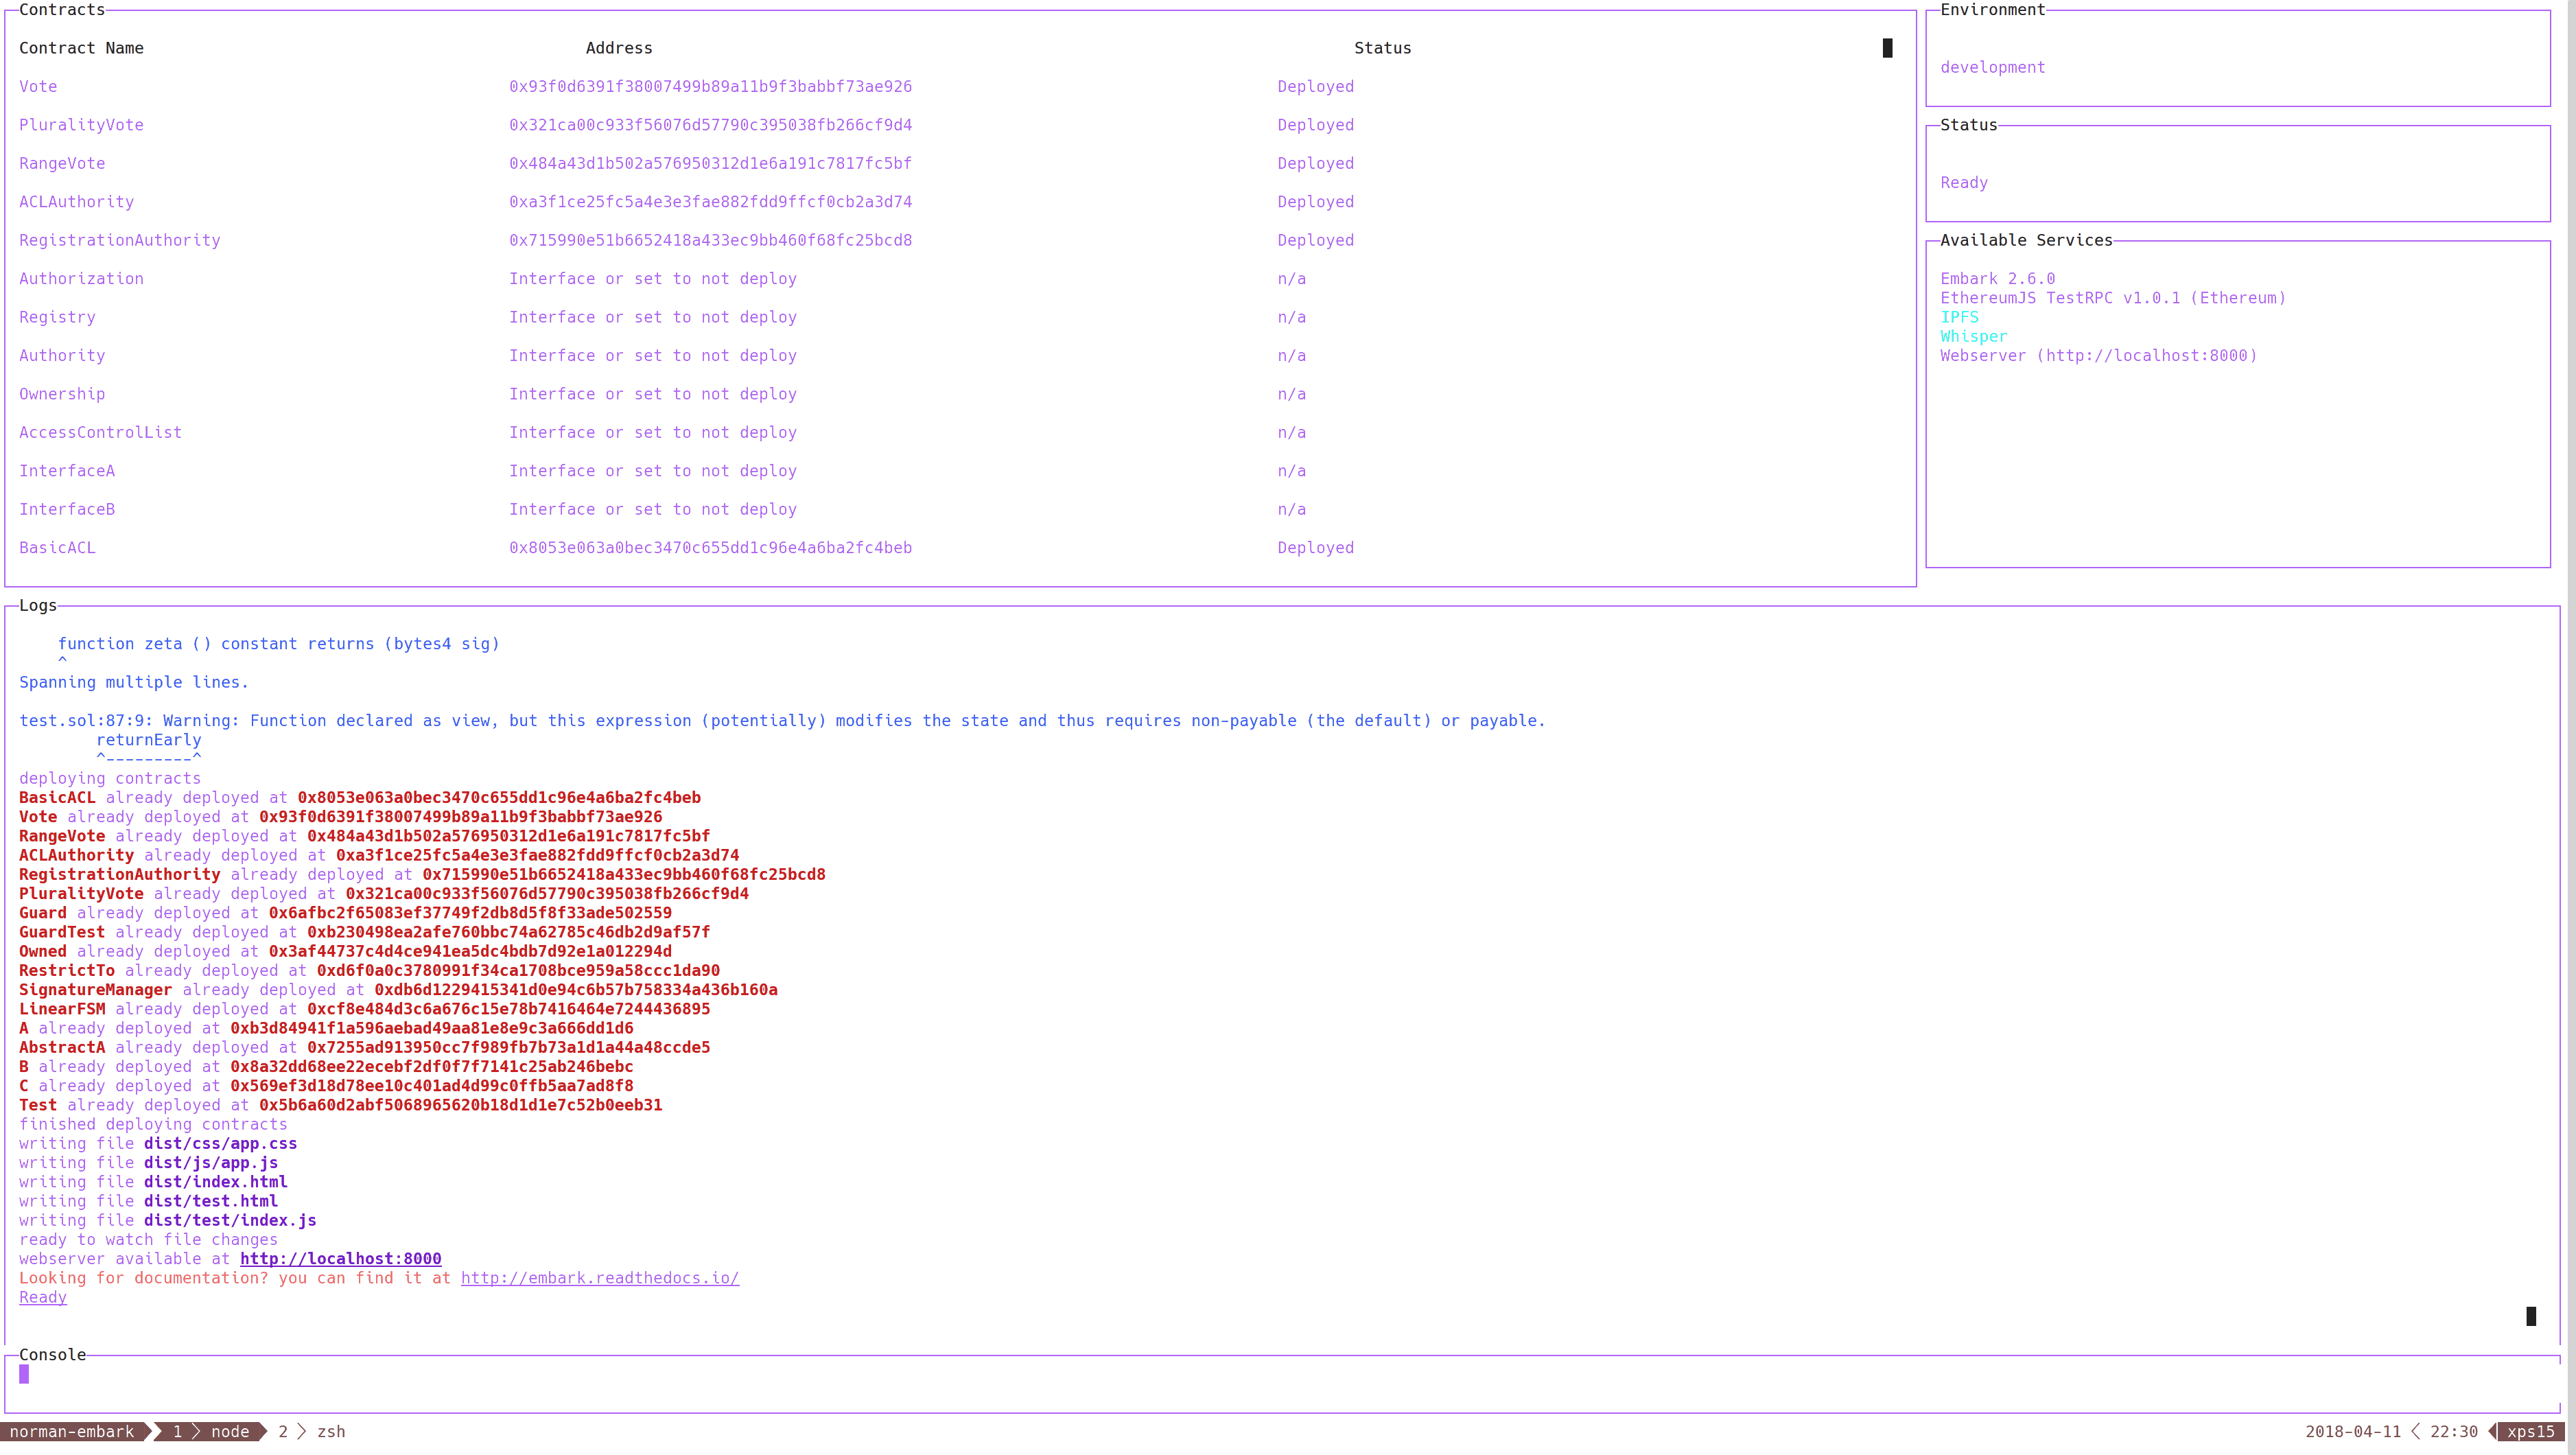
\includegraphics[width=\textwidth]{embark-ui-transparent-bg}
  \caption{The Embark dashboard and application state.}\label{fig:embark-dashboard}
\end{figure}


\subsubsection{Truffle}
Later smart contract development was completed using the Truffle framework. When
compared to the contract development features of the Embark Framework, the
Truffle framework can be viewed as an almost feature-identical framework ---
i.e., smart contract lifecycle management, testing functionality, JavaScript
bindings, and network management --- however, unlike the Embark framework, the
Truffle framework offers essentially no features related to DApp development.
The Truffle framework's more targeted focus with regards to smart contract
development and management produced a cleaner development experience during the
pursuit of this research, which is concerned strictly with smart contract design
and implementation and not DApp development. Furthermore, the Truffle framework
supports executing workflows and tests in TypeScript, and can be used in
conjunction with \solt{TypeChain} to generate TypeScript types for use with the
smart contract bindings generated by Truffle. A screenshot displaying the
execution of a contract test via the Truffle framework can be seen in
Figure~\ref{fig:truffle-test}.

\begin{figure}[H]
  \centering
  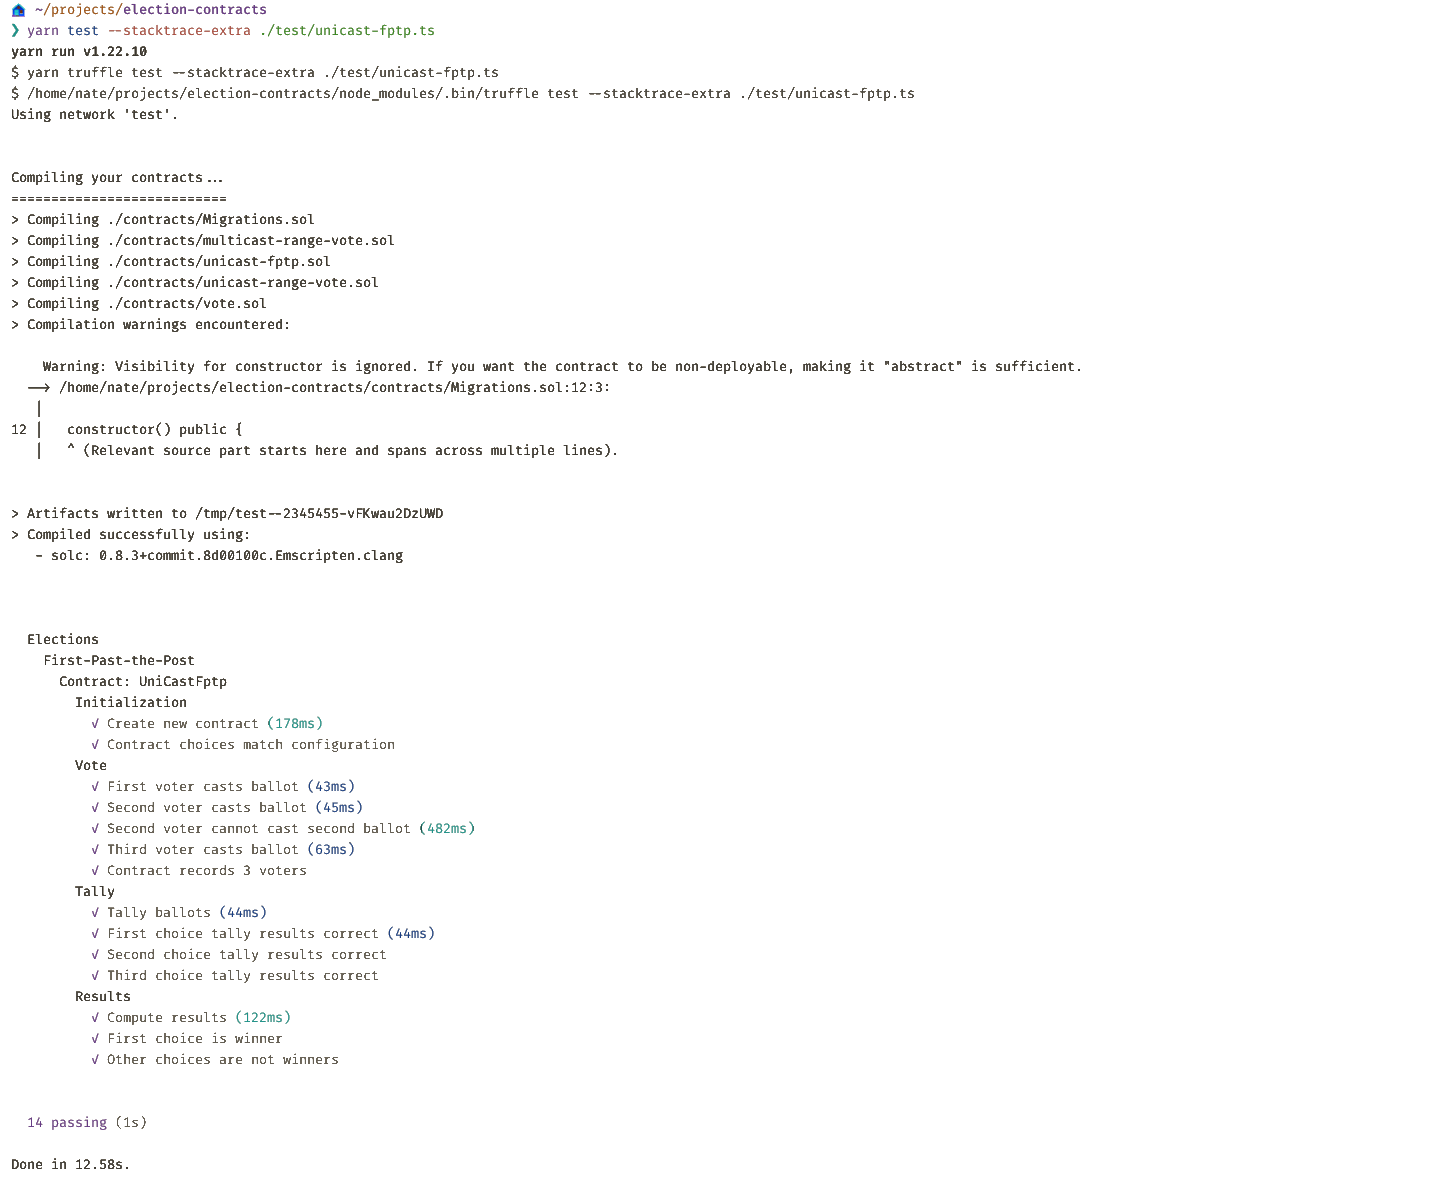
\includegraphics[width=\textwidth]{truffle-test-transparent-bg}
  \caption{Testing an election contract using the Truffle framework.}\label{fig:truffle-test}
\end{figure}

% seemed to result in to  i.e., lifecycle management, contract testing and
% debugging,


% Section: Design
\section{Architecture and Design}\label{sec:architecture-and-design}
The design of the system is approached in three phases: authorization, election,
and delegation. Each phase considers different components of the overall system
architecture and each component is responsible for managing a different set of
responsibilities within the architecture.

% system. The authorization components, delegation components, and election
% components.

% , henceforth collectively referred to as Norman.

% The Embark framework --- a framework designed to build Decentralized
% Applications (DApps) --- is used to provision test networks, build, deploy,
% and test the components. The Embark framework can manage and deploy to
% different chains, e.g., testnet, private net, and livenet. Embark
% automatically detects changes to contracts, builds, and then deploys the
% contracts onto the appropriate Ethereum networks. To build Solidity code into
% EVM code the Embark framework uses solcjs which offers JavaScript bindings for
% the Solidity compiler. For expedited development and testing Embark exposes
% the Ethereum JavaScript testrpc which simulates a fully functioning Ethereum
% client. Interaction with Ethereum contracts is simplified by automatically
% generating promise-based JavaScript functions which expose contract functions.
% JavaScript support is provided by wrapping the web3js library which implements
% the generic Ethereum JSON RPC spec. Embark also supports decentralized storage
% via IPFS, decentralized messaging through Whisper and Orbit, and a curses-like
% dashboard which exposes logs, environment, contract states, available
% services, a console, and the status of the framework generally.

\begin{center}
  \figurepdf{venn-diagram}
  % \includestandalone{\fig{venn-diagram}}
\end{center}

\subsection{Authorization Components}
The authorization components are designed to provide access control: to build
and maintain a set of eligible voters, administrators, and whatever other roles
might be necessary to implement the electoral systems. Ultimately, the
authorization components are responsible for restricting access to sensitive
contract function calls that mutate the state of the contract, e.g., casting
ballots and configuration elections. The design must be flexible enough to
facilitate the varying and evolving needs of different organizations and
communities but consistent enough to support them all through a common
interface. Concepts are borrowed from traditional operating system access
control schemes/models and authorization mechanisms which provide guidance for
system design. The underlying authentication features are handled via the
asymmetric cryptography provided by the underlying blockchain infrastructure.

\subsubsection{Access Control}
Access control schemes exist to authorize access to data and resources; they are
responsible for managing and defining the relationships between permissions,
operations, objects, and subjects. Several access control model schemes were
considered in this phase; among them were: access control lists, discretionary
access control, mandatory access control, and role-based access control.

\paragraph{Discretionary Access Control}
Discretionary Access Control (DAC) is a form of access control where the owner
of some resource/object can dictate the operations and permissions that other
subjects can take on the resource/object. Additionally, the owner of the
resource/object can pass ownership to some other subject. You can see a form of
this in POSIX file systems where ownership over files is granted and transferred
through commands like \codet{chown} and \codet{chmod}.

\paragraph{Access Control Lists}
An Access Control List (ACL) is a collection of \emph{subject}, \emph{resource},
and \emph{permission} relationships which can be understood as a matrix, where
each cell, indexed by \emph{subject} and \emph{resource}, reflects the
\emph{permissions} available for the \emph{subject} to access \emph{resource}.

% \todo{Intersection? Corresponding?}

\paragraph{Role-Based Access Control}
Role-Based Access Control (RBAC) is a form of access control where collections
of permissions are assigned to roles; roles are then assigned to users. In RBAC
roles are hierarchical, thus roles can be inherited from parent roles.

% Word semantic?
\subsubsection{Design}
The fundamental resources exposed by smart contracts are function calls, thus
the security implementation and access control model must revolve around that.
We define an interface, \sol{Authority}, which defines the \sol{canCall}
function. Any contract wishing to implement access control on functions can
leverage a contract that implements the \sol{Authority} interface to authorize
access to those functions.

\begin{figure}[H]
  \centering
  \figurepdf[width=\textwidth]{authorization}
  % 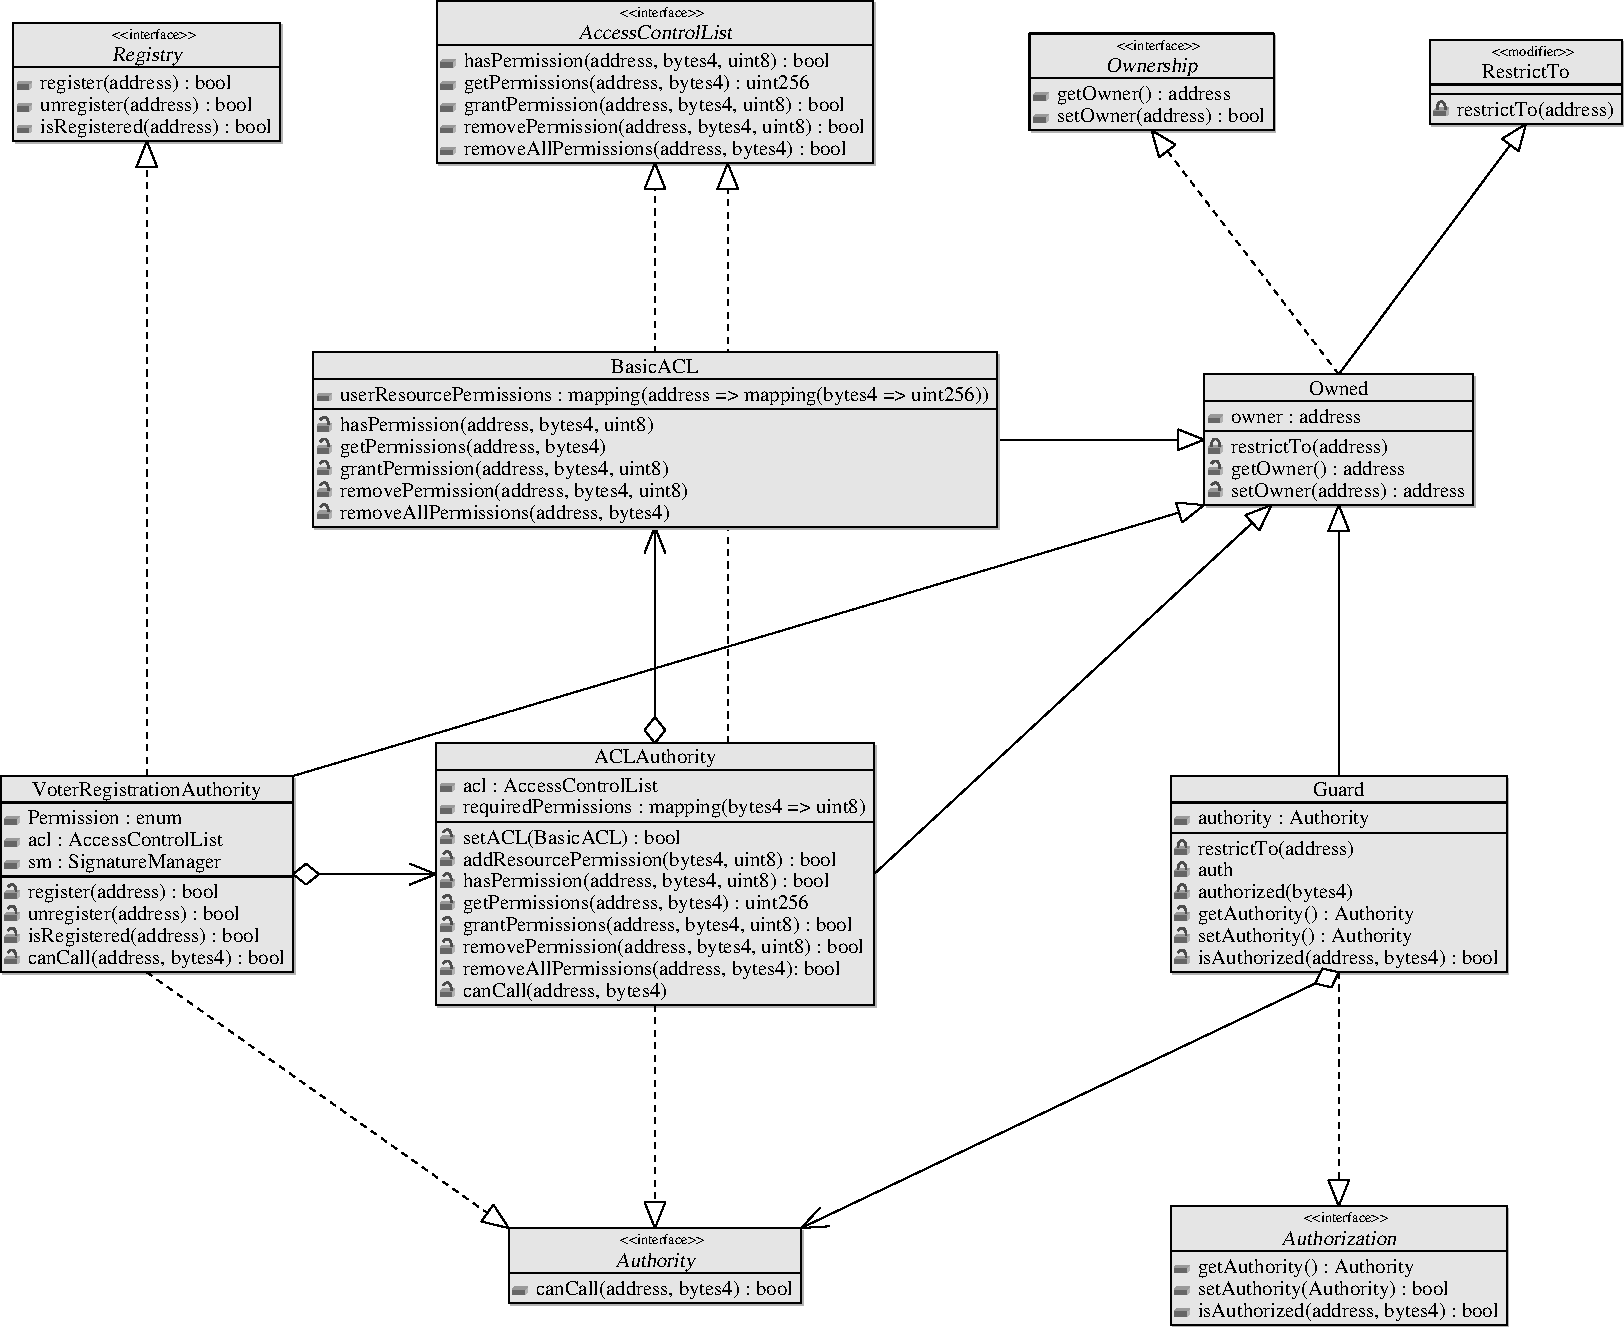
\includegraphics[width=\textwidth]{figures/authorization/figure}
  % \includestandalone[width=\textwidth]{\fig{authorization}}
  \caption{Authorization dependency graph modeling.}\label{fig:authorization}
\end{figure}

We define the \sol{Authorization} interface which offers mechanisms for
interacting with an \sol{Authority}. This interface defines \sol{getAuthority},
\sol{setAuthority}, and most importantly, \sol{isAuthorized}. A contract that
realizes the \sol{Authorization} interface is expected to aggregate an
\sol{Authority} but does not necessarily need one externally; for example, a
contract that provides \sol{Authorization} may also be its own \sol{Authority}.
Likewise, an \sol{Authority} can provide its own \sol{Authorization}. The
\sol{Authority} and \sol{Authorization} interfaces together form our access
control primitives.

The \sol{Guard} contract realizes the \sol{Authorization} interface and provides
the modifier functions \sol{auth} and \sol{authorized}. These can be applied to
other functions to easily restrict function-call access to accounts that the
\sol{Authority} has approved, e.g.,

\begin{solidity}[Guard Usage Example]
function sensitive () public auth returns (bool _success) {
  // The `auth` modifier prevents this function from being
  // called until the Authority has confirmed that the
  // the message sender has the proper privileges.
  return true;
}
\end{solidity}

This implementation conforms to a number of design principles: separation of
concerns, dependency inversion principle, open/closed principle, interface
segregation, substitution principle, and single responsibility principle.
Ultimately it provides the flexibility and resiliency necessary to build out a
wide variety of electoral systems.

\paragraph{Ownership}
Access control often starts before our \sol{Authority} and \sol{Authorization}
realizations. Most contracts offer a primitive form of access control through
\sol{Ownership}. All contracts and most contract functions are open and public
by design; thus, it is important to lock down sensitive contract functions from
deployment. A common pattern is to store the \solt{address} of the creator of a
contract as an owner in the contract state and to use that address to restrict
access to sensitive public-facing functions. More complicated ownership
mechanisms can be built using this pattern by leveraging contracts which
delegate ownership to another contract which can then define more complex access
control and management mechanisms. To facilitate in this and many other useful
patterns we introduce a simple \sol{Ownership} interface. The \sol{Ownership}
interface defines functions \sol{getOwner} and \sol{setOwner} which get and set
the account address of a contract's owners respectively.

To facilitate in restricting access of functions to a single account we also
define a contract \sol{RestrictTo} that provides a modifier function
\sol{restrictTo}. The \sol{restrictTo} modifier can be applied to any other
function and takes an account address argument; if the address of the account
calling a \sol{restrictTo} modified function does not match the argument
provided to \sol{restrictTo} (often the owner), then the function will
immediately exit and revert any changes to the contract. Finally, we realize and
extend these two contracts to form the concrete \sol{Owned} contract. This
pattern is so ubiquitous that most, if not all, concrete contracts in our
governance ecosystem will extend this contract.

\paragraph{Authority}
We need to provide access control beyond interfaces, standards, and single
account address restrictions. Our access control implementation leans towards
access control lists as a primitive that can be extended to provide other access
control mechanisms such as role-based access control. Alternatively, a contract
can realize the \sol{Authority} interface itself if ACLs are not a useful
abstraction.

\subparagraph{Access Control List}
We first define an ACL interface, \sol{AccessControlList}, which defines basic
ACL functionality: \sol{hasPermission}, \sol{getPermissions},
\sol{grantPermission}, \sol{removePermission}, and \sol{removeAllPermissions}.
The design supports assigning up to 256 unique permissions per contract
signature.

\subparagraph{Basic ACL}
Next we realize a concrete implementation of the \sol{AccessControlList}
interface named \sol{BasicACL}. \sol{BasicACL} is primarily a
database contract which creates a mapping from account address to a mapping of
functions (the first 4 bytes of their signature) to an unsigned 256-bit integer
that represents the permissions. This implementation is similar to what can be
found in POSIX compliant operating systems. In Java one might represent this
access control model as \codet{HashMap<Account, HashMap<Function,Permission>>}.

Naturally \sol{BasicACL} provides implementations for the functions defined by
\sol{AccessControlList}: \sol{hasPermission}, \sol{getPermissions},
\sol{grantPermission}, \sol{removePermission}, and \sol{removeAllPermissions}.
These work using bitwise NOT, OR, and AND operations to modify the 256-bit
unsigned integer representing permissions for a particular (account, function)
pair.

\subparagraph{ACL Authority}
We can easily build an \sol{ACLAuthority} out of our \sol{BasicACL} using the
adapter pattern and aggregation. We simply aggregate an instance of a
\sol{BasicACL} and realize the \sol{Authority} and \sol{AccessControlList}
interfaces. Finally, we lean on the \sol{hasPermission} function to implement
our \sol{canCall} function which presumably forwards our request to a
\sol{BasicACL} instance and returns the result. This structure also allows us to
implement a composite pattern and aggregate many trusted authorities into one.

\subparagraph{Voter Registration Authority}
Our final step is to use a facade to hide the more complex implementation
details from outside contracts. We introduce a \sol{VoterRegistrationAuthority}
which realizes the \sol{Registry} and \sol{Authority} interfaces.
The \sol{Registry} interface provides some nice abstractions:
\sol{register}, \sol{unregister}, and \sol{isRegistered}. We
presume the contract aggregates some number of \sol{AccessControlList}s as
a foundation for its \sol{Registry} function implementations, but does not
need to necessarily. Finally, the \sol{canCall} function leans on the
\sol{Registry} functions, specifically \sol{isRegistered} to grant
access to functions.

The end result is a clean, public, and composable voter registration authority.


\subsection{Election Components}
The election components are responsible for constructing and operating election
processes. These responsibilities include maintaining the integrity and security
of the election, handling votes, tallying ballots, and determining election
winners.

The phases typically involved in conducting an Internet-based election,
described in Section~\ref{sec:internet-voting}, are: Setup, Distribution,
Voting, Casting, Tallying, and Auditing. Responsibilities pertaining to voter
registration, which are typically handled in the Setup phase, are expected to be
managed by Authorization components. The Distribution phase, which mostly
pertains to processes such as mailing election materials to voters, is
considered outside the scope of this research and therefore ignored. The
Auditing phase, where election integrity and results are scrutinized, is assumed
to be handled and provided by the underlying features made available by
Ethereum.

% Ideally the ballots would be recorded separately from the tallying method. If
% they were we could apply different tallying methods to the same set of ballots
% and produce different results. Unfortunately it's extremely costly to store
% ballots as part of the contract state.

% We opt for first-past-the-post and range vote for single-winner elections, the
% former for its simplicity and ubiquity, the latter for its effectiveness. This
% provides an implementation of a plurality voting system and majority voting
% system.

\subsubsection{Design}
Each electoral system implementation is unique, due mostly to the unique
requirements necessitated by their underlying tallying algorithms and ballot
structures.

There are important electoral criteria worth considering when analyzing the
implementation feasibility of these electoral systems, namely, the ballot
counting criteria: summability, polynomial time, and resolvable. These electoral
criteria are significant because they impact the gas costs associated with
operating the electoral system. Table~\ref{tab:criteria-compliance} is a useful
resource when considering these electoral criteria. Both the first-past-the-post
and range vote electoral systems are a 1\textsuperscript{st}-order summable;
i.e., ballots can be tallied using a linear amount of space with respect to the
number of choices available without losing information required to complete the
tallying processes. Both also have polytime ballot counting implementations that
are linear in the number of candidates and voters. STV is not listed in the
table; however, its single-winner equivalent (IRV) is; which implies that STV
has, at best, a tallying complexity of $O(n^2)$ and a summability complexity
of $O(n!)$ with respect to the number candidates.

Gas costs must be considered when implementing, deploying, and running contract
functions on the Ethereum Virtual Machine (EVM). If gas costs are too high then
it may become infeasible for an external account to afford to execute a contract
function, e.g., the network fees become too high to vote. Another concern to
consider is that the cost to execute a contract function may become too high to
ever complete in a single block, therefore never actually complete. The most
expensive operations, by no small margin, are operations involving storage.
Therefore it is important to minimize storage usage.

% Fortunately these EVM limitations map well
% to many voting method criteria. We can lean on these criteria and the field of
% computational social choice theory broadly to restrict the set of voting systems
% to just the ones that can be feasibly implemented on the Ethereum blockchain.

\paragraph{Finite State Machine}
Several of the voting system designs use a phased approach with timed
transitions between election states: Configuration, Frozen, Vote, and Tally.
These phases can be modeled as a finite state machine where calls to various
functions trigger transitions to different stages. A modifier function can be
used to restrict access of functions to only be callable during their
appropriate state. Most of the transitions from state to state can be designed
as timed transitions which occur lazily, i.e., the check to confirm that it is
time to transition from one state to another occurs when a function is called.
The rationale for this approach is due to the fact that Ethereum offers no
mechanism to trigger code execution \emph{from within the blockchain itself};
therefore all function calls, even if called from another function or even a
function in a different contract, must ultimately have originated from a
transaction created by an externally owned account. The product of this timed
transition implementation implies that the state restriction modifier needs to
occur after the lazily evaluated timed transition modifier; i.e., first update
the current state if it should be, then validate if the function should
executed. On the other hand, if transitions are manually updated during a
function's execution then the opposite behavior should occur; i.e., first
validate if the function should be run, then update the state as required.

\subparagraph{Configuration}
The Configuration phase, as implied by the name, exists to provide election
administrators an opportunity to configure the election contract: choices,
election start/end time, etc. After the configuration is complete the
administrators can freeze the contract, preventing it from being modified
further.

\subparagraph{Frozen}
Transitioning to the Frozen phase could simply set a boolean \sol{frozen} to
true and update the phase to Frozen. The boolean \sol{frozen} should be checked
at the start of every administrative function's execution and should cause the
immediate cease of code execution if the value is true. This serves to prevent
potentially malicious election administrators from modifying an election
contract after the voting process has started; it also serves to notify external
contracts and users that the election is configured and is ready or waiting to
move into the Vote phase.

\subparagraph{Vote}
The Vote phase is the phase during which various kinds of voting can occur for a
particular election contest. A \sol{vote} function should be defined. For
flexibility, a \sol{vote (uint8[], uint8[])} function signature is considered
which is capable of being leveraged by most kinds of electoral systems and
ballot structures. For example, as a sparse vector, where both arrays are of
equal length; values in the first array act as a choice index and values from
the second array act as a choice value. This could be used to marginally reduce
the size of transactions for many kinds electoral systems.

\subparagraph{Tally}
The Tally phase is the final phase of the election process that takes place
after the end of the Voting phase. The exact tallying process will depend on the
electoral system itself.


\paragraph{First-Past-the-Post}
The process for a first-past-the-post election is as follows:

\begin{enumerate}
  \item Configuration
  \begin{enumerate}
    \item Election administrators add each contest choice: \\
      \sol{addChoice(bytes32 _choice)}.
    \item Election administrators set the voting start time: \\
      \sol{setVoteStartTime(uint _voteStartTime)}.
    \item Election administrators set the voting end time: \\
      \sol{setVoteEndTime(uint _voteStartTime)}.
    \item Election administrators freeze the electoral contract, preventing
      further contract configuration mutations: \sol{freeze()}.
  \end{enumerate}

  \item Frozen
  \begin{enumerate}
    \item All functions are disabled until start time is met.
  \end{enumerate}

  \item Vote
  \begin{enumerate}
    \item Authorized voters cast votes by calling the \sol{vote(uint8 _choice)}
      function, where the value provided is the choice the voter supports.
      Votes are immediately summed into the struct of the appropriate choice.
      This is feasible because the first-past-the-post electoral system is
      summable in linear time and with linear space consumption.
  \end{enumerate}

  \item Tally
  \begin{enumerate}
    \item When the voting end time is reached the election moves into the
      Tally phase. At this point only the tally function can be called.
      The tally function, in this case, will check the number of votes for
      each candidate and set the winner to the choice that has received
      the most support. The election administrator is expected to run this
      contract function but any account can execute this function without
      any consequence to the result of the contract.
  \end{enumerate}
\end{enumerate}

\paragraph{Range Voting}
The process for a range vote is very similar to the process for
first-past-the-post. It is as follows:

\begin{enumerate}
  \item Configuration
  \begin{enumerate}
    \item Election administrators add each contest choice: \\
      \sol{addChoice(bytes32 _choice)}.
    \item Election administrators set the voting start time: \\
      \sol{setVoteStartTime(uint _voteStartTime)}.
    \item Election administrators set the voting end time: \\
      \sol{setVoteEndTime(uint _voteStartTime)}.
    \item Election administrators set the max score (<=100) a choice can
      receive: \\
      \sol{setMaxScore(uint8 _maxScore)}.
    \item Election administrators freeze the electoral contract, preventing
      further contract configuration mutations: \sol{freeze()}.
  \end{enumerate}

  \item Frozen
  \begin{enumerate}
    \item All functions are disabled until start time is met.
  \end{enumerate}

  \item Vote
  \begin{enumerate}
    \item Authorized voters cast votes by calling the \sol{vote(uint8[] _choices, uint8[] _scores)}
      function. The parameters act as a sparse vector where the value
      provided in \sol{_choice} indicates the choice being scored
      and the corresponding value provided in \sol{_scores}
      indicates the score of the choice. Scores are immediately summed
      into the struct of of the appropriate choice and a
      \sol{voteCount} member is incremented. This is feasible
      because the range vote electoral system is summable in linear time
      and with linear space consumption.
  \end{enumerate}

  \item Tally
  \begin{enumerate}
    \item When the voting end time is reached the election moves into the
      Tally phase. At this point only the tally function can be called.
      The tally function for this electoral system will, for each choice,
      multiply the summed score by $10^p$ where $p$ is
      \sol{precision} then divide the result by
      \sol{voteCount} to find an average score for the choice. The
      winner is set to the choice with the highest average score. The
      score is multiplied by $10^p$ because the EVM does not have floating
      point functionality and a greater precision makes ties less likely.
      The election administrator is expected to run this contract function
      but any account can execute this function without any consequence to
      the result of the contract.
  \end{enumerate}
\end{enumerate}



\subsection{Delegation Components}
The delegation components offer mechanisms for the electorate to vest votes to
delegates who may vote on their behalf. A delegation hierarchy lends itself to a
graph representation.\cite{delegative-democracy} Specifically a directed
acyclic graph (DAG) forest-like structure where pendant and isolated vertices
represent voters and all other vertices represent delegates. A sink vertex
represents a delegate who has not delegated their vote further. Directed edges
represent delegations. The total weight of a voter, their voting power, can be
measured by recursively calculating the total number of incoming edges for each
vertex. We represent edges in the graph as follows:

% \begin{displayquote}
%   In a large and complex organization, the generalist role --- merely knowing
%   who knows best about something --- is often as important a function as the
%   specialist role of being able to make good decisions in any particular area.
%   In traditional large democratic structures, where elected officials in key
%   positions manage a hierarchical bureaucracy of some kind, most of those
%   elected positions are effectively generalist positions by practical necessity.
%   Ordinary voters do not have the interest level or patience required for
%   electing appropriate people to a large number of specialist positions, and
%   most would not have the knowledge or connections required to make good
%   decisions about those positions anyway. Therefore, specialists can usually
%   only participate in a large organization by being appointed or hired into a
%   position in the un-elected bureaucracy, and for this reason people are always
%   effectively subservient to the generalists who choose them. For this reason
%   the entire field of ``politics'' has effectively become a profession of
%   generalists, which very little technical knowledge in any particular field is
%   required or expected (except perhaps law), but in which the most important
%   characteristic of a candidate is the ability to look good, speak well, and
%   make the right connections. But it seems unfortunate and problematic that all
%   specialists are effectively excluded from direct participation in the
%   democratic process except in role that are strictly subservient to the
%   generalists: at the very least this structural pathology certainly contributes
%   to the frequently observed tendency of politicians to ``legislate'' highly
%   technical issues without adequate consultation with the experts in the
%   appropriate technical field --- or with a selection of ``experts'' that is
%   highly skewed for political reasons --- often with disastrous results.
%   Delegative democracy with open specialized forums and re-delegation provides
%   an alternative structure that enables both generalists and specialists to
%   participate directly in the democratic process as first-class policy-makers.
%   Widely recognized and trusted generalized are given the legitimate ability to
%   affect the balance of power in specialized forums by directing delegated votes
%   to chosen specialists, while the specialists participating directly in those
%   forums also retain the ability to build their own independent power bases and
%   thus not be completely at the mercy of generalists. At the same time, since
%   generalists and specialists alike are direct participants in the democratic
%   process, they have the same fundamental rights and responsibilities and are
%   all held accountable to all of their constitutes (i.e., those who delegate
%   votes to them) in the same way.
% \end{displayquote}

\begin{solidity}[Delegation Structure]
struct Voter {
  uint40 weight; // 5 bytes
  address delegate; // 32 bytes
}
\end{solidity}

Each time a delegation occurs a depth first traversal should be performed to
ensure that no cycles are created by the delegation; doing so maintains the
acyclic invariant required of the graph to support voter delegation. A simple
graph coloring algorithm is considered, beginning with white vertices and
coloring vertices black as they are traversed; traversal starts from the vertex
representing the voter who is delegating their vote and ends at some sink
vertex. If no cycle is detected the algorithm should check to see if the voter
has already delegated their vote; if so, it should traverse down their current
delegation path, decreasing the weight of each vertex visited by the weight
of the voter or delegate delegating their vote. Finally, the algorithm should
record the new delegate address and perform a final traversal, following the
same path originally traversed while performing cycle detection, increasing the
weight of each vertex visited along the way by the weight of the voter or
delegate delegating their vote. More briefly:
\begin{enumerate}
  \item Confirm that there are no cycles within the new delegation chain.
  \item Decrease the weight of the delegates in the old delegation chain.
  \item Increase the weights of the delegates in the new delegation chain.
\end{enumerate}
A complete implementation of this algorithm is as follows:\footnotemark{}

\footnotetext{
  Here we assume that every voter has their voting weight initialized to 1. This
  algorithm might be improved by combining the cycle detection and weight
  accumulation steps while leveraging the \sol{revert()} function to revert the
  state of the contract if a cycle is detected. We opt not to do that for now
  because return values are not currently available with the \sol{revert()}
  functionality.
}

\begin{solidity}[Vote Delegation]
mapping (address => Voter) voters;

function delegateVote (address delegate) public auth returns (bool _success) {
  // The `auth` modifier prevents this function from being
  // called until the Authority has confirmed that the
  // the message sender has the proper privileges.
  Voter cursor;
  uint40 weight = voters[msg.sender].weight;

  mapping (address => bool) visited;
  visited[msg.sender] = true;
  visited[delegate] = true;

  // Cycle Detection
  cursor = voters[delegate];
  while (cursor.delegate) {
    address newDelegate = cursor.delegate;
    if (visited[newDelegate]) return false;
    cursor = voters[newDelegate];
    visited[newDelegate] = true;
  }

  // Decrement weights of old delegate chain.
  cursor = voters[msg.sender];
  while (cursor.delegate) {
    address newDelegate = cursor.delegate;
    cursor = voters[newDelegate];
    cursor.weight -= weight;
  }

  // Increment weights of new delegate chain.
  cursor = voters[msg.sender];
  cursor.delegate = delegate;
  while (cursor.delegate) {
    address newDelegate = cursor.delegate;
    cursor = voters[newDelegate];
    cursor.weight += weight;
  }

  return true;
}
\end{solidity}





% Section: Testing
% \section{Test Results}\label{sec:test-results}
Testing Ethereum contracts can be approached in several ways, but the choices
one can make with regards to testing mostly align themselves into one of two
categories: the driver which is executing the contract being tested and the
network environment the contract is being tested within.


\begin{enumerate}
  \item The test driver generally comes in one of two shapes:

    \begin{enumerate}
      \item Contract-to-contract unit tests, which use tests written as smart
        contracts to drive contract execution. These tests provide confidence
        that inter-contract communication will function as expected.

      \item Client-to-contract unit tests, which use transactions generated by
        external accounts to drive contract execution. These tests provide
        confidence that external accounts can run contract code as expected.
    \end{enumerate}

  \item The network environment comes in several shapes, listed from least
    realistic to most:

    \begin{enumerate}
      \item The \codet{testrpc}, now deprecated, is a Node.js-based Ethereum
        client which simulates a full client and network behavior. It is free to
        execute and fast, but lacks the complexities of a real node.

      \item Ganache, which replaces \codet{testrpc} and is functionally
        identical from a testing perspective.

      \item One can run a local instance of Ethereum. This is is free and
        accurately represents an Ethereum node, but lacks real-world network
        complexities.

      \item There are several ``testnets,'' which are test networks designed for
        actual contract deployments. Testnets provide a close-to-reality network
        environment while still providing a free means of acquiring funds for
        testing.

      \item The most accurate environment to test in is the actual Ethereum
        network; this is not free, but offers a perfect real-world environment
        to test contracts in.
    \end{enumerate}
\end{enumerate}

% Testing Ethereum contracts comes in a few flavors: contract-to-contract and
% client-to-contract tests which can occur on various blockchain networks:
% testrpc, local blockchain, testnet, and livenet.
%
% Contract-to-contract unit tests are used to ensure that contract code can be run
% by internal accounts as expected. Client-to-contract unit tests are used to
% ensure that external accounts can run contract code as expected. Developing
% using the \codet{testrpc} simulates a blockchain network, it is free and fast,
% but lacks the complexities of a real node. Running a local blockchain instance
% is free, accurately represents an Ethereum node, but lacks real-world network
% complexities. The testnet is a test network designed for actual Ethereum
% contract deployments, it accurately simulates much of the network infrastructure
% and traffic while still providing free means of acquiring funds for testing. The
% final stage of testing is deploying code onto the actual Ethereum network, this
% is not free but offers a real-world environment to test contract code.
%
% The tests for Norman are client-to-contract tests with contracts deployed using
% the testrpc, on a local blockchain, and on the testnet. Mocha is used as a
% JavaScript testing framework, EmbarkJS is used to provide a JavaScript interface
% to contract code, and Chai is used as an assertion library.

The tests built in this research leverage the \codet{testrpc} and Ganache as
development and testing environments, generally launched as either
\codet{ganache-cli --accounts 100 --networkId 7357} or \codet{testrpc --gasLimit
0xffffffff --port 8546}. Tests were driven through JavaScript and TypeScript
contract bindings using the Embark and Truffle frameworks respectively.

\subsection{Election Components}
Several election contracts were implemented with various modifications to their
implementations based on their underlying electoral system and features being
targeted. Each election contract accepts a configuration object containing the
choices available for the election along with various other properties based on
the requirements of the underlying electoral system. Additional details
regarding implementation are available in Appendix~\ref{appendix:documentation}.


\subsubsection{Election Simulation}

To generate estimates regarding the cost of execution and storage required to
support features of electoral systems, several sets of elections were simulated
using various configurations of contract implementation, choice availability,
ballot structure, and voter selection. The general process required producing
minimal implementations of each electoral system and modifying them as necessary
to explore the advantages and disadvantages of various design choices. Each
electoral system implementation then had minimal tests written to validate that
basic functionality was present, then simulations implemented. Each simulation
leveraged hundreds of accounts which were generated for our test network using
Ganache. Each account, to the extent supported by the underlying electoral
system, made random voting choices: selecting and scoring candidates through
pseudorandom number generation.

\begin{spacing}{1.2}
  % \caption{Gas consumption as measured by contract and simulation.} \\
  \small
  \begin{longtabu} to \textwidth{X[l] X[1,r] X[0.3,c] X[0.4,r] X[0.75,r] X[0.75,r]}
      \caption{Simulated gas consumption by contract function.} \\
      \toprule
      Contract           & \multicolumn{2}{r}{{Operation}} &      & \multicolumn{2}{r}{{Gas Consumption}}   \\
                         \cmidrule(lr){2-3}        \cmidrule(lr){5-6}
                         & Function       & Call & Voters & Total            & Average              \\
      \midrule
      \endhead
      UniCastFptp        & vote           &    1 &    100 &  \num{8007700}   & \num{80077}          \\
      UniCastRangeVote   & vote           &    1 &    100 &  \num{17417564}  & \num{174175}         \\
      MultiCastFptp      & vote           &    1 &    100 &  \num{7447632}   & \num{74476}          \\
      MultiCastFptp      & vote           &    2 &    100 &  \num{3208496}   & \num{32084}          \\
      MultiCastRangeVote & vote           &    1 &    100 &  \num{23266645}  & \num{232666}         \\
      MultiCastRangeVote & vote           &    2 &    100 &  \num{9525039}   & \num{95250}          \\

      UniCastFptp        & tally          &    1 &      1 &  0               & 0                        \\
      UniCastRangeVote   & tally          &    1 &      1 &  \num{149356}    & \num{149356}             \\
      MultiCastFptp      & tally          &    1 &      1 &  \num{917790}    & \num{917790}             \\
      MultiCastRangeVote & tally          &    1 &      1 &  \num{5342859}   & \num{5342859}            \\

      UniCastFptp        & computeResults &    1 &      1 &  \num{360516}    & \num{360516}             \\
      UniCastRangeVote   & computeResults &    1 &      1 &  \num{47416}     & \num{47416}              \\
      MultiCastFptp      & computeResults &    1 &      1 &  \num{47438}     & \num{47438}              \\
      MultiCastRangeVote & computeResults &    1 &      1 &  \num{47394}     & \num{47394}              \\
      \bottomrule\label{tab:election-simulations}
  \end{longtabu}
\end{spacing}
% \footnotetext{
%   These values were generated by taking the average gas consumption observed
%   over several simulation runs. Simulations were configured using 100 voters in
%   each run, with 10 available choices to select from in each election, and a
%   random ballot submission process. The tally and results of each election were
%   validated independently alongside the contract's results.
%   % \begin{enumerate}[leftmargin=5mm,topsep=0mm]
%   %   \item These values are from several simulation runs using 100 voters and a
%   %     random ballot submission process.
%   % \end{enumerate}
% }

% \footnotemark{}
Table~\ref{tab:election-simulations} documents the result of contract
simulations, mapping gas consumption by election contract function. These values
were generated by measuring the total gas consumption observed over several
simulation runs and computing the average cost per contract function.
Simulations were configured using 100 voters in each run, with 10 available
choices to select from in each election. A random choice selection and
evaluation process was used to generate ballots used to  vote. The tally and
results of each election were validated independently alongside the contract's
results.

\paragraph{Ballot Storage and Tallying Algorithms}

Section~\ref{sec:elections} introduced concepts regarding ballot structure and
tallying algorithm. Section~\ref{sec:electoral-criteria} further-refined
these ideas while introducing the ballot counting criteria: polytime,
resolvable, and summability. To measure the significance of these criteria and
the impact of various ballot formats on our overall design, several
implementations of FPTP and range vote were implemented and simulated.

\begin{enumerate}
  \item \sol{UniCastFptp} is an implementation of first-past-the-post which was
    designed to permit a single ballot to be cast per voter. This implementation
    takes advantage of the summability criterion to avoid storing each
    individual voter's ballot and instead maintains a continuous tally of the
    ballots. The space required is therefore constant with respect to the number
    of voters and linear with respect to the number of candidates whose
    \solt{vote_counts} are being tallied.

  \item \sol{UniCastRangeVote}, like \solt{UniCastFptp}, is an implementation
    of range vote designed to only allow a single ballot to be cast per voter.
    This implementation again takes advantage of the summability criterion to
    avoid storing each individual voter's ballot and instead maintains a
    continuous tally of the ballots. The range vote implementation needs to
    store slightly more information to support its tallying algorithm, but
    shares the same storage complexity as the \solt{UniCastFptp} implementation.
\end{enumerate}

% \paragraph{Multi-vote Functionality}
The \sol{UniCastFptp} implementation demonstrated a \emph{very} consistent gas
consumption across its function calls through the exercised simulations.
The \solt{UniCastRangeVote} implementation maintained a slightly less consistent
gas consumption across function calls, but stayed respectably stable.

\subparagraph{Multi-Vote Functionality and Tallying Algorithms}
The functional requirements laid out in Section~\ref{sec:requirements} and
Table~\ref{tab:research-requirements} demand multi-vote support. Two contracts
were written to demonstrate this functionality.

\begin{enumerate}
  \item \sol{MultiCastFptp}, an implementation of first-past-the-post designed
    to permit a voter to cast multiple ballots.

    % This implementation takes advantage of the summability criterion to avoid
    % storing each individual voter's ballot and instead maintains a continuous
    % tally of the ballots. The space required is therefore constant with respect
    % to the number of voters and linear with respect to the number of candidates
    % whose \solt{vote_counts} are being tallied.

  \item \sol{MultiUniCastRangeVote}, like \solt{MultiCastFptp}, is an
    implementation of range vote designed to allow multiple ballots to be cast
    per voter.

    % This implementation again takes advantage of the summability criterion to
    % avoid storing each individual voter's ballot and instead maintains a
    % continuous tally of the ballots. The range vote implementation needs to
    % store slightly more information to support its tallying algorithm, but
    % shares the same storage complexity as the \solt{UniCastFptp}
    % implementation.
\end{enumerate}

It is clear that a voter's ability to cast multiple ballots in an election could
only be considered fair if the principle of ``one person, one vote'' were
adhered to. That is to say, any ballot which has been submitted and had some
partial tally applied based on its marks \emph{must} have its computations
undone before a newer ballot's marks can be considered for tallying. The ability
to cast multiple ballots therefore carries with it an implied requirement of
vote reversal. In order to reverse a previous ballot's impact on a tally,
knowledge of the ballot's marks is required. Therefore, the most recent ballot
of each voter must be maintained in the contract's state to support
vote-reversal in the incident that they cast multiple ballots.

This draws into question the viability and utility of leveraging the summability
criterion as a storage-saving feature, as was leveraged in the previous
contracts, and introduces questions with regard to the \emph{eager evaluation vs
lazy evaluation} of tallying algorithms. The unicast implementation of each
electoral system took advantage of eager evaluation, which essentially forced
each voter to pay a nominal amount of extra gas to keep the current tally of
each choice maintained, this is reflected in
Table~\ref{tab:election-simulations} by the low gas cost associated with the
unicast \solt{tally} functions (0 in the case of \sol{contract UniCastFptp}!).
The more traditional approach to tabulating results in an election is to defer
the tallying procedure until the end of the voting period and have an election
administrator incur the cost and responsibility of tallying ballots. This was
the approach taken in the multicast implementations of these two contracts;
however, it is worth noting that a middle-ground exists which would increase the
cost to vote by a nominal amount and result in a less-expensive tally cost.

One interesting outcome regarding ballot storage and storage costs is reflected
in Table~\ref{tab:election-simulations}; there is a  dramatic reduction in gas
costs incurred when casting a second ballot. The high initial gas cost reflects
the high charge incurred for consuming storage space on the blockchain. The
lower cost reflected by the second call is a product of the new ballot replacing
the old ballot in storage, therefore consuming no additional space on the
blockchain.

\paragraph{Precision Decision and Casting Fake Ballots}
Each electoral system has advantages and disadvantages. It is the responsibility
of those selecting and designing such systems to attempt to balance those
advantages and disadvantages in a reasonable way. Two examples of this
encountered during this research can be seen in the range vote implementations.
The range vote implementation requires the following configuration to be
provided during contract construction:

\begin{solidity}[RangeVoteConfiguration]
struct RangeVoteConfiguration {
  string[] choices;
  RangeVoteConfigurationFakeBallots fake_ballots;
  uint8 min_range;
  uint8 max_range;
  uint8 tally_precision;
}

struct RangeVoteConfigurationFakeBallots {
  uint8 score;
  uint40 voter_count;
}
\end{solidity}

The \sol{tally_precision} value is worth addressing. The tallying algorithm used
to determine the rank of a choice in a range vote election is computed by taking
the summation of all of the scores cast for the choice and dividing that
summation by the number of voters who ranked the choice. This produces a score
average which is used to determine the winner of an election. One weakness of
the EVM is that floating point operations are not supported; in order to address
that a tally precision is used, which multiplies the \solt{score_sum} by
$10^{tally\_precision}$ before dividing it to maintain some degree of precision.
What an appropriate value to assign to \sol{tally_precision} is will depend on
the specifics of the election.

Another value worth addressing is the \solt{struct} \sol{fake_ballots} property.
One weakness of the range vote electoral system is that naive implementations
can result in elections where unknown alternatives, being neither voted for or
against, win elections again more popular alternatives; imagine voting for
oneself in a large election, and being the only person to, therefore winning the
election with a perfect score average. One common technique to avoid this kind
of result in range vote implementations is for election administrators to agree
ahead of time to some number of fake ballots to be cast. These fake ballots will
score each choice with the same rank, typically 0, and therefore bias results
towards choices which have received enough votes to overcome the low scores
received from the fake ballots.

\paragraph{Modeling Finite-State Machine Transitions}
Election contract's state transitions were tested by creating and conducting
mock elections to ensure that the results are as expected. Passage of time in
the \codet{testrpc} is simulated using the \sol{evm_increaseTime} RPC
method.\cite{testrpc}

\begin{itemize}
  \item \textbf{First-Past-the-Post} The tests for the First-Past-the-Post
    electoral system are as follows:
    \begin{enumerate}
      \item Generate a First-Past-the-Post instance.
      \item Test that the owner and creation time are properly initialized.
      \item Confirm that the phase is \sol{Configuration}.
      \item Add two choices to be voted for.
      \item Set the voting start time.
      \item Set the voting end time.
      \item \sol{freeze} the contract so that no further configuration can occur.
      \item Confirm that the contract is \sol{Frozen}.
      \item Increase the time of the EVM such that the contract's
        \sol{timedTransitions} will trigger and move the contract into the
        \sol{Vote} phase on the first ballot submission.
      \item Generate a set of Ethereum accounts and vote for the choices.
      \item Monitor the cast ballots to confirm that the votes are submitted as
        expected.
      \item Confirm that the phase is \sol{Vote}.
      \item Increase the time of the EVM such that the contract's
        \sol{timedTransitions} will trigger and move the contract into the
        \sol{Tally} phase.
      \item Loop over the choices to find the winner.
      \item Confirm that the winner is the expected winner.
      \item Confirm that the phase is \sol{Tally}
    \end{enumerate}

  \item \textbf{Range Vote} The tests for the Range Vote electoral system are as
    follows:
    \begin{enumerate}
      \item Generate a Range Vote instance.
      \item Test that the owner and creation time are properly initialized.
      \item Confirm that the phase is \sol{Configuration}.
      \item Add three choices to be voted for.
      \item Set the voting start time.
      \item Set the voting end time.
      \item \sol{freeze} the contract so that no further configuration can occur.
      \item Confirm that the contract is \sol{Frozen}.
      \item Increase the time of the EVM such that the contract's
        \sol{timedTransitions} will trigger and move the contract into the
        \sol{Vote} phase on the first ballot submission.
      \item Generate a set of Ethereum accounts and vote for the choices.
      \item Monitor the cast ballots to confirm that the votes are submitted as
        expected.
      \item Confirm that the phase is \sol{Vote}.
      \item Increase the time of the EVM such that the contract's
        \sol{timedTransitions} will trigger and move the contract into the
        \sol{Tally} phase.
      \item Loop over the choices to find the winner.
      \item Confirm that the winner is the expected winner.
      \item Confirm that the phase is \sol{Tally}
    \end{enumerate}
\end{itemize}

\subsection{Authorization Components}
There are a number of contracts that need testing that revolve around
authorization, the most important being the \sol{VoterRegistrationAuthority},
\sol{Guard}, \sol{ACLAuthority}, and \sol{BasicACL}.

\paragraph{Voter Registration Authority}
The tests for the \sol{VoterRegistrationAuthority} are as follows:
\begin{enumerate}
  \item Generate a set of external voting accounts.
  \item Deploy an instance of the \sol{VoterRegistrationAuthority}.
  \item Register a subset of the voting accounts with the
    \sol{VoterRegistrationAuthority}.
  \item Verify that the registered voting accounts return true when passed to
    \sol{isRegistered}.
  \item Verify that the unregistered voting accounts return false when passed to
    \sol{isRegistered}.
  \item Unregister a subset of the registered voting accounts.
  \item Verify that the registered voting accounts return true when passed to
    \sol{isRegistered}.
  \item Verify that the unregistered voting accounts return false when passed to
    \sol{isRegistered}.
\end{enumerate}

\paragraph{Guard}
The \sol{Guard} is tested using the previously deployed
\sol{VoterRegistrationAuthority} as an \sol{Authority}. A \sol{TestGuard}
instance is tested by attaching an \sol{auth} modifier to a dummy \sol{vote}
function. The \sol{vote} function is then tested by confirming that each of the
verified voting accounts can call the \sol{vote} function. Each unregistered
account is also tested to confirm that none of those accounts can call the
\sol{vote} function.

% TODO:
% Words:
% Authority
% Secure
% Authorize
% Authenticate
% Security
% SecureContract
% Firewall
% Privilege
% Verify

% \subsection{Election Components}
% Election contracts are tested by creating and conducting mock elections to
% ensure that the results are as expected. Passage of time in the testrpc is
% simulated using the \sol{evm_increaseTime} RPC method.
%
% \subsubsection{First-Past-the-Post}
% The tests for the First-Past-the-Post electoral system are as follows:
% \begin{enumerate}
%   \item Generate a First-Past-the-Post instance.
%   \item Test that the owner and creation time are properly initialized.
%   \item Confirm that the phase is \sol{Configuration}.
%   \item Add two choices to be voted for.
%   \item Set the voting start time.
%   \item Set the voting end time.
%   \item \sol{freeze} the contract so that no further configuration can occur.
%   \item Confirm that the contract is \sol{Frozen}.
%   \item Increase the time of the EVM such that the contract's
%     \sol{timedTransitions} will trigger and move the contract into the
%     \sol{Vote} phase on the first ballot submission.
%   \item Generate a set of Ethereum accounts and vote for the choices.
%   \item Monitor the cast ballots to confirm that the votes are submitted as
%     expected.
%   \item Confirm that the phase is \sol{Vote}.
%   \item Increase the time of the EVM such that the contract's
%     \sol{timedTransitions} will trigger and move the contract into the
%     \sol{Tally} phase.
%   \item Loop over the choices to find the winner.
%   \item Confirm that the winner is the expected winner.
%   \item Confirm that the phase is \sol{Tally}
% \end{enumerate}
%
% \subsubsection{Range Vote}
% The tests for the Range Vote electoral system are as follows:
% \begin{enumerate}
%   \item Generate a Range Vote instance.
%   \item Test that the owner and creation time are properly initialized.
%   \item Confirm that the phase is \sol{Configuration}.
%   \item Add three choices to be voted for.
%   \item Set the voting start time.
%   \item Set the voting end time.
%   \item \sol{freeze} the contract so that no further configuration can occur.
%   \item Confirm that the contract is \sol{Frozen}.
%   \item Increase the time of the EVM such that the contract's
%     \sol{timedTransitions} will trigger and move the contract into the
%     \sol{Vote} phase on the first ballot submission.
%   \item Generate a set of Ethereum accounts and vote for the choices.
%   \item Monitor the cast ballots to confirm that the votes are submitted as
%     expected.
%   \item Confirm that the phase is \sol{Vote}.
%   \item Increase the time of the EVM such that the contract's
%     \sol{timedTransitions} will trigger and move the contract into the
%     \sol{Tally} phase.
%   \item Loop over the choices to find the winner.
%   \item Confirm that the winner is the expected winner.
%   \item Confirm that the phase is \sol{Tally}
% \end{enumerate}

% \subsection{Delegation Components}
% \todo{Finish documenting the delegation contract tests.}

% \section{Authentication Contract}
% The role of the Authentication Contract is to build and maintain a set of
% eligible voter's (whitelist), ineligible voter's (blacklist), and Authentication
% Contract authorities' (publisher's) public keys. Note that this is similar to
% the signing of keys to build a web of trust.
%
% Beyond a whitelist there should also be some sort of technique to
% (???automatically generate???) private keys (BIP-0032 comes to mind).
%
% \emph{TODO:\ Should this be generated using recursive ``signing'' contracts
% (building a Web-of-Trust)? One global signing contract could maintain a
% collection of (public key, signing contract) pairs. Each signing contract could
% only be updated by the private key associated with the public key that created
% the contract and would itself maintain a list of public keys that it considers
% legitimate.}
%
% \emph{TODO:\ Merkle tree to store the state of the contract at a particular
% block? Used to get a static version of valid keys.}
%
% \subsection{Functionality}
%
% \begin{center}
% \resizebox{\columnwidth}{!}{%
%     \begin{tabu} to \textwidth{@{} l l l @{}}
%         \toprule
%         \textbf{Key}    & \textbf{Type}     & \textbf{Description} \\
%         \midrule
%         name            & String            & A name for this authentication contract. \\
%         admins          & Set<Key>          & A collection of authentication contract administration officials' public keys. \\
%         dkg\_key        & Key               & A public key generated by authentication officials using a DKG process. \\
%         seed\_start     & Integer           & The starting key permitted to be generated by the DKG\_Key. \\
%         seed\_end       & Integer           & The ending key permitted to be generated by the DKG\_Key. \\
%         whitelist       & Set<Key>          & A collection of authorized keys. \\
%         blacklist       & Set<Key>          & A collection of unauthorized keys. \\
%         \bottomrule
%     \end{tabu}
% }
% \end{center}
%
% \paragraph{Functionality 1: Creation}
% A collection of authentication administrators create an Authentication Contract:
% register their public keys, perform a DKG process (publish the public key),
% and collectively add/remove users from the whitelist, blacklist, and
% publisher list.
%
% The number of election officials required for each of these operations should be
% variable --- e.g., 2-of-N, 3-of-N;\ where *N* is the total number of election
% officials.
%
% \emph{TODO:\ Is the DKG process necessary in this case? It will probably need to
% be recomputed for every new administrator added/removed and does not seem to
% provide a value add. The DKG public key could be used for the deterministic key
% generation.}
%
% \paragraph{Functionality 2: Whitelist}
% The whitelist offers a means of adding individual public keys. This is useful
% for small authentication contracts and exceptions in the case of seed, but
% should probably be avoided in large-scale contracts.
%
% One nice feature of a whitelist is that the private key is never known to the
% authentication contract administrators.
%
% \paragraph{Functionality 3: Deterministic Keys}
% The deterministic generation of valid keys is an important convenience feature
% for the authentication contract administrators (and optimization feature with
% respect to the blockchain). This feature would allow administrators to
% deterministically generate and whitelist public keys without actually needing to
% write them into the blockchain (similar to BIP-0032). 3rd party contracts could
% validate and verify public keys by performing the same deterministic
% computations as the election officials.
%
% This feature implies that there be additional \lstinline|seed_start| and
% \lstinline|seed_end| values which would limit the range of valid deterministically
% generated public keys. \lstinline|seed_start| and \lstinline|seed_max| could be updated
% by election administrators.
%
% Ultimately this functionality would provide a lost-cost and effective means
% of adding swaths of keys into the whitelist without actually needing to write to
% the blockchain (writing data into the blockchain is an expensive operation
% [?]).
%
% One negative consequence of this technique is that private keys probably need to
% be distributed by authentication contract administrators, perhaps by mail. This
% leaves open some attack vectors; BIP-0032-like functionality might help to track
% down attacks, but couldn't prevent them.
%
% \paragraph{Functionality 4: Blacklist}
% The blacklist offers a means of removing individual public keys from the
% contract, e.g., in the case of lost keys, death, or compromised keys. The
% blacklist should take priority over the whitelist and the deterministically
% generated keys, i.e., \emph{no public key in the blacklist should ever be considered
% valid}.
%
% \paragraph{Functionality 5: Administrator List}
% The authentication contract administrators should be able to add and remove
% members to and from the collection of administrators. This is perhaps the most
% risky operation when compared to the others. Administrators should be heavily
% vetted as the integrity of the authentication contract depends on their
% diligence and maintenance. Thusly, the addition of new members to the
% authentication contract should probably require a supermajority approval from
% other authentication administrators. This approval process should be public in
% order to track down discovered corruption.
%
% \emph{TODO:\ The addition/removal of contract officials implies that the DKG process
% needs to be re-run. This impacts the public/private key deterministic generation
% process. The key generation and administration addition/removal process needs to
% be more carefully considered.}
%
% \section{Proxy Contract}
% The Proxy Contract enables voters to delegate their vote to another voter.
%
% \subsection{Functionality}
%
% \begin{center}
% \resizebox{\columnwidth}{!}{%
%     \begin{tabu} to \textwidth{@{} l l l @{}}
%         \toprule
%         \textbf{Key}        & \textbf{Type}     & \textbf{Description} \\
%         \midrule
%         name                & String            & A name for this proxy (Science, Economics, Social). \\
%         auth\_contract      & Contract          & The authentication contract which contains the set of eligible voters. \\
%         parent\_proxy       & Contract          & The parent proxy contract of this proxy contract (hierarchical proxy capability). \\
%         proxies             & Set<Key>          & A collection of public keys which have agreed to act as proxies. \\
%         election\_contract  & Contract          & An election contract with proxies as options. \\
%         \bottomrule
%     \end{tabu}
% }
% \end{center}
%
% {Note: The \lstinline|auth_contract| and \lstinline|parent_proxy| contract are mutually exclusive.}
%
% {Note: The root \lstinline|parent_proxy| must contain an \lstinline|auth_contract|.}
%
% \paragraph{Functionality 1: Proxy Consent}
% To become an eligible proxy you must first consent to act as a proxy. This is
% done by calling \lstinline|proxy.consent()| with a valid public key from
% \lstinline|auth_contract|.
%
% \emph{TODO:\ Merkle tree to store the state of the contract at a particular block?
% Used to get a static version of valid keys.}
%
% \paragraph{Functionality 2: Create Election}
% Register a new election with all proxies and parent proxies as choices in the
% election. If an election already exists then the election should pre-seed with
% the encrypted votes from the previous proxy election (effectively keeping
% previous delegations).
%
% \section{Election Contract}
% The role of the Election Contract is to build and run elections as well as
% ensure the integrity and security of its elections and participating actors. A
% number of cryptographic and cryptoeconomic incentivization-disincentivization
% schemes are used to maintain election integrity and security.
%
%
% \subsection{Functionality}
%
% \begin{center}
% \resizebox{\columnwidth}{!}{%
%     \begin{tabu} to \textwidth{@{} l l l @{}}
%         \toprule
%         \textbf{Key}        & \textbf{Type}                 & \textbf{Description} \\
%         \midrule
%         administrators      & Set<Key>                      & A set of public keys associated with each of the administration officials of the election. \\
%         DKG\_key            & Key                           & A public key generated by election officials using a DKG process. \\
%         name                & String                        & A name for this election (Minimum Wage, Proxy, New Cafeteria Food). \\
%         description         & String                        & A short description of this election. \\
%         choices             & Set<String>                   & A set of choices. \\
%         start\_time         & Unsigned Integer              & The start time of the election. \\
%         end\_time           & Unsigned Integer              & The end time of the election. \\
%         proxy\_time         & Unsigned Integer              & The time all proxy votes have to be in by. \\
%         write\_in           & Boolean                       & Allow write-in ballots (default: false).\\
%         auth\_contract      & Contract                      & The authentication contract which contains the set of eligible voters. \\
%         proxy\_contract     & Contract                      & The proxy contract that applies to this election. \\
%         mixnet\_nodes       & Set<Key>                      & A set of public keys associated with each of the nodes in the mixnet. \\
%         mixnode\_fee        & Unsigned Integer              & The cost associated with becoming a mixnet node. \\
%         proxy\_ballot       & Map<Key, PlaintextBallot>     & A mapping of authenticated proxy voter's public keys to their plaintext ballots. \\
%         voter\_ballot       & Map<Key, EncryptedBallot>     & A mapping of authenticated voter's public keys to their encrypted ballots. \\
%         \bottomrule
%     \end{tabu}
% }
% \end{center}
%
% \paragraph{Functionality 1: Creation}
% A quorum of election officials form to administer the election contract. The
% quorum of election officials register their public keys, perform a DKG process
% (publish the public key), and collectively configure the election parameters:
% \lstinline|name|, \lstinline|description|, \lstinline|choices|, \lstinline|start_time|, \lstinline|end_time|, \lstinline|proxy_time|,
% \lstinline|proxy_contract|, and \lstinline|auth_contract|.
%
% Election officials must each individually submit good faith deposits (security
% deposits), binders to the election contract which will be forfeited should the
% election decryption stage fail. Their binders collectively should sum to enough
% ether to reimburse each voter in case of election failure. Should decryption
% fail all election official's deposits will be forfeited.
%
% Officials will be rewarded for administering the election process if the
% election proceeds without dishonesty.
%
% \emph{TODO:\ Could we have a bidding process here for the decryption step?}
% \emph{TODO:\ Separate administration from decryption.}
%
% \paragraph{Functionality 2: Mixnet Node Registration}
% Immediately after the creation of the election contract a bidding process
% begins and continues to run until the \lstinline|end_time| of the election. Bidders bid
% in the bidding process to become nodes in the mixnet. The five highest bidders
% are selected as nodes in the mixnet. The starting bid is the cost to run the
% election.
%
% The bids act as good faith deposits, binders to the election contract which will
% be forfeited should the mixnet node be found guilty of dishonesty.
%
% Election officials are collectively guaranteed up to three nodes in the mixnet.
% Each node could of course be a mixnet itself.
%
% 8 nodes total? Configurable?
%
% The election officials use a
%
% \emph{TODO:\ Is an exponential bidding process viable?}
%
% \emph{TODO:\ We should probably just use the 5 highest bidders. We'll just fall victim
% to a Sybil attack if we try to do some partitioning of bidders to allow cheaper
% bidders into the game and randomly select from them. It's functionally identical
% to the highest bidder winning.}
%
% \emph{TODO:\ 5 and 5 was a completely arbitrary choice. This probably isn't necessary
% for a low stakes election. This should probably be determined based on number of
% voters and election administrator configuration.}
%
% \paragraph{Functionality 3: Submit Ballot --- Proxy}
% Proxy voters, proxies, can submit plaintext votes using an account
% associated with their authorized public key.
%
% After the \lstinline|proxy_time| has passed proxies can no longer vote using their proxy
% ballot. If they have not committed to a proxy ballot before the \lstinline|proxy_time|
% then they are eligible to vote using a voter ballot.
%
% *Note: Proxies can only vote with the votes that have been delegated to them, not
% their own vote; e.g., Bob and Charlie both delegate their vote to Alice, Alice
% can now vote with a weight of 2 (Bob and Charlie's vote), not 3 (she's lost her
% own vote). Further, only proxies can submit votes using proxy ballots. Both of
% these properties exist to maintain receipt freedom freedom.
%
% Another way to imagine this is as a tree of voters, where the leaves of the tree
% give weight to the vote and the non-leaf nodes influence the direction/choice of
% the vote.*
%
% *Note: We need to have a static version of the proxy so that voters cannot
% remove their proxy vote and vote again; and so that proxies cannot vote, then
% remove their proxy status, then vote again.*
%
% \paragraph{Functionality 4: Submit Ballot --- Voter}
% If a voter has not submitted a proxy ballot then a voter may submit a ballot
% encrypted using the DKG public key produced by the election administrators.
% Ballots are encrypted using an El Gamal encryption scheme which provides
% re-encryption and additive homomorphic features.
%
% \paragraph{Functionality 5: Verification}
% For a week after the election, verifiers, for a charge, can challenge the mixnet
% nodes. If a mixnet node does not respond in a timely fashion to each of the
% challenges then the mixnet node is accused of dishonesty and their binder is
% forfeit. The dishonest mixnet node is booted from the mixnet and the mixnet is
% rerun. 40\% of the dishonest node's good faith deposit is given given to the
% verifier of the election as a reward for discovering the dishonesty. 30\% of the
% dishonest node's deposit is burned, and the last 30\% of the deposit is put into
% the reward pool for the election which is split between election administrators
% and honest mixnet nodes.
%
% \emph{TODO:\ Should voters be given some of the reward?}
%
% The verification functionality is broken into two parts: commitment,
% verification, and collection.
%
% \subparagraph{Commmit}
% The verifier commits to challenging a mixnet node by submitting a transaction
% containing a hash of verification challenge parameters, the node that they wish
% to challenge, a reward address, and a deposit (enough gas/ether to verify the
% transaction on chain). An immutable mapping is created that links the hash of
% the verification parameters to the reward address.
%
% \subparagraph{Verify}
% After the verifier is sufficiently convinced that their hash is set in the
% blockchain they can activate the verification process by revealing their
% challenge parameters, a portion of the mix node proof, and the necessary merkle
% tree elements to confirm the legitimacy. The verification parameters are
% computed against the mixnet node's published proof to detect dishonesty. The
% previously mentioned mixnet node punishment occurs if dishonesty is discovered.
%
% *Note: If they verifier never reveals their verification parameters then their
% deposit is forfeit and added to the contract reward pool.*
%
% \paragraph{Final Notes}
% Receipt freedom might be compromised if an organization large enough proxies
% their votes individually to people they wish to coerce or vote buy from.
%
% Mixnode attack to delay election.
%
% Verifier attack to refund money in mixnode delay attack.
%
% \section{Stages}
% As seen above the Election Contract depends on the Authentication Contract
% and/or Proxy Contract, however it is useful to understand the voting system
% beginning with the Election.
%
% \begin{figure}[H]
%     \centering
%     \caption{Stages of election.}\label{fig:blockchain}
%     \includestandalone[width=\textwidth]{\fig{stages}}
% \end{figure}
%
% \begin{enumerate}
%     \item Creation
%         \begin{enumerate}[a.]
%             \item Election administrators perform a distributed key generation
%                 process to generate an ElGamal key pair that supports additive
%                 homomorphic properties.
%             \item The public key is published to the election contract.
%         \end{enumerate}
%     \item Configuration
%         \begin{enumerate}[a.]
%             \item Election administrators add additional election administrators
%                 to the contract.
%             \item Election administrators set the authentication contract.
%             \item Election administrators set the proxy contract.
%             \item Election administrators configure the start time of the
%                 election contract.
%             \item Election administrators configure the end time of the election
%                 contract.
%             \item Election administrators configure the end time for delegate
%                 voting.
%             \item Election administrators configure the number of mixnet nodes
%                 they will operate.
%             \item Election administrators configure the number of mixnet nodes
%                 that will be available for bidders to bid for.
%             \item Election administrators freeze the configuration process. No
%                 additional configurations are accepted by the contract after
%                 this point. This signals the bidding process for external mixnet
%                 participants.
%         \end{enumerate}
%     \item Voting Begins
%         \begin{enumerate}[a.]
%             \item Voting begins at the start time specified by election
%                 administrators.
%             \item Delegates must publish their ballots unencrypted to leverage
%                 votes that have been delegated to them. Note that delegates
%                 forfeit their own vote to leverage their constituent's votes.
%         \end{enumerate}
%     \item Proxy Voting Ends
%         \begin{enumerate}[a.]
%             \item Proxy voting has ended. Voters now have an opportunity to
%                 override their proxy's public vote by publishing an encrypted
%                 ballot. Note that delegates who have published an unencrypted
%                 ballot have locked themselves in, they can no longer vote as a
%                 normal voter.
%         \end{enumerate}
%     \item Voting Ends
%         \begin{enumerate}[a.]
%             \item Proxy voting has ended. Voters now have an opportunity to
%                 override their proxy's public vote.
%         \end{enumerate}
%     \item Mixnet Cycle
%         \begin{enumerate}[a.]
%             \item The top n bidders, where n is the number of external mixnet
%                 nodes available for bid, with the highest bids are selected as
%                 the external nodes to participate in the mixnet process. (Should
%                 a blinding process happen? e.g., Ethereum Name Service bidding)
%             \item A node ordering is determined from the set of available nodes
%                 to perform a mix. The nodes are picked using a pseudo random
%                 selection process based off of the hash of the most recent block
%                 (should we use a block from a few back in case another chain is
%                 used?).
%         \end{enumerate}
%     \item Publish Mixnet Proof
%         \begin{enumerate}[a.]
%             \item Each mixnet node publishes their mixed ballots and a proof of
%                 mix. If a node does not publish their required outputs in the
%                 required amount of time they are removed from the mixnet and the
%                 next mixnet node takes their place.
%         \end{enumerate}
%     \item Verification Begins
%         \begin{enumerate}[a.]
%             \item Proof of subproduct
%             \item Any individual or organization willing to verify the proofs
%                 may do so by publishing a challenge and paying an appropriate
%                 fee. If mixnet nodes don't respond within a reasonable time
%                 frame they are removed from the mixnet and the mixnet cycle
%                 restarts.
%         \end{enumerate}
%     \item Tally Results
%         \begin{enumerate}[a.]
%             \item Encrypted votes are tallied together using the additive
%                 homomorphic property.
%         \end{enumerate}
%     \item Decryption Cycle
%         \begin{enumerate}[a.]
%             \item Election administrators come together to generate the private
%                 key and decrypt the tallied votes.
%         \end{enumerate}
%     \item Publish Decryption Proof
%         \begin{enumerate}[a.]
%             \item Election administrators publish their proof of decryption. If
%                 this is not published in the required amount of time the
%                 election fails.
%         \end{enumerate}
%     \item Verification Ends
%         \begin{enumerate}[a.]
%             \item After some period of time passes to allow verifiers to
%                 challenge the decryption proof and mixnet proofs the election
%                 ends.
%         \end{enumerate}
% \end{enumerate}
%
% Notes:
% \begin{itemize}
%     \item Bidders must publish a public key as part of the bidding process.
%     \item Mixnet nodes must remain available for challenges during the entire
%         verification period.
% \end{itemize}
%
%
% \section{Ballot Format}


\chapter{Results}\label{chap:results}

This chapter outlines the results of this research.
%
% produced in the process of implementing the
% authorization, election, and delegation components introduced in
% Section~\ref{sec:architecture-and-design}; provides benchmarks, test results,
% cost, and complexity analysis.
%
This chapter is divided into two major sections:

\begin{enumerate}
  \item \emph{Test Results}, which reviews significant benchmarks, test results,
    and operational costs discovered in the design and implementation of this
    research.

  \item \emph{Analysis}, which uses the requirements and criteria, targeted in
    Section~\ref{sec:requirements}, and objectives targeted in
    Section~\ref{sec:objectives}, to measure the shortcoming and results of this
    research and also reviews insights and unexpected challenges encountered
    during the implementation phase.
\end{enumerate}

% Section: Testing
% \section{Implementation}
% After initial design the implementation of each component was approached
% independently.

%
% The procedure used to implement each of the components related to the election
% contracts occurred as follows:
%
% \begin{enumerate}
%   \item An exploration of Finite State Machine design to manage transitioning
%     between the various voting phases.
%
%   \item Rudimentary implementations of each electoral system were implemented.
%
%     \begin{enumerate}
%       \item Tests were implemented to validate the basic functionalities of the
%         election contract and the correctness of the results produced by the
%         underlying electoral system implementation: voting, ballot tallying, and
%         winner selection process.
%     \end{enumerate}
%
% \end{enumerate}

% Section: Testing
\section{Test Results}\label{sec:test-results}
Testing Ethereum contracts can be approached in several ways, but the choices
one can make with regards to testing mostly align themselves into one of two
categories: the driver which is executing the contract being tested and the
network environment the contract is being tested within.


\begin{enumerate}
  \item The test driver generally comes in one of two shapes:

    \begin{enumerate}
      \item Contract-to-contract unit tests, which use tests written as smart
        contracts to drive contract execution. These tests provide confidence
        that inter-contract communication will function as expected.

      \item Client-to-contract unit tests, which use transactions generated by
        external accounts to drive contract execution. These tests provide
        confidence that external accounts can run contract code as expected.
    \end{enumerate}

  \item The network environment comes in several shapes, listed from least
    realistic to most:

    \begin{enumerate}
      \item The \codet{testrpc}, now deprecated, is a Node.js-based Ethereum
        client which simulates a full client and network behavior. It is free to
        execute and fast, but lacks the complexities of a real node.

      \item Ganache, which replaces \codet{testrpc} and is functionally
        identical from a testing perspective.

      \item One can run a local instance of Ethereum. This is is free and
        accurately represents an Ethereum node, but lacks real-world network
        complexities.

      \item There are several ``testnets,'' which are test networks designed for
        actual contract deployments. Testnets provide a close-to-reality network
        environment while still providing a free means of acquiring funds for
        testing.

      \item The most accurate environment to test in is the actual Ethereum
        network; this is not free, but offers a perfect real-world environment
        to test contracts in.
    \end{enumerate}
\end{enumerate}

% Testing Ethereum contracts comes in a few flavors: contract-to-contract and
% client-to-contract tests which can occur on various blockchain networks:
% testrpc, local blockchain, testnet, and livenet.
%
% Contract-to-contract unit tests are used to ensure that contract code can be run
% by internal accounts as expected. Client-to-contract unit tests are used to
% ensure that external accounts can run contract code as expected. Developing
% using the \codet{testrpc} simulates a blockchain network, it is free and fast,
% but lacks the complexities of a real node. Running a local blockchain instance
% is free, accurately represents an Ethereum node, but lacks real-world network
% complexities. The testnet is a test network designed for actual Ethereum
% contract deployments, it accurately simulates much of the network infrastructure
% and traffic while still providing free means of acquiring funds for testing. The
% final stage of testing is deploying code onto the actual Ethereum network, this
% is not free but offers a real-world environment to test contract code.
%
% The tests for Norman are client-to-contract tests with contracts deployed using
% the testrpc, on a local blockchain, and on the testnet. Mocha is used as a
% JavaScript testing framework, EmbarkJS is used to provide a JavaScript interface
% to contract code, and Chai is used as an assertion library.

The tests built in this research leverage the \codet{testrpc} and Ganache as
development and testing environments, generally launched as either
\codet{ganache-cli --accounts 100 --networkId 7357} or \codet{testrpc --gasLimit
0xffffffff --port 8546}. Tests were driven through JavaScript and TypeScript
contract bindings using the Embark and Truffle frameworks respectively.

\subsection{Election Components}
Several election contracts were implemented with various modifications to their
implementations based on their underlying electoral system and features being
targeted. Each election contract accepts a configuration object containing the
choices available for the election along with various other properties based on
the requirements of the underlying electoral system. Additional details
regarding implementation are available in Appendix~\ref{appendix:documentation}.


\subsubsection{Election Simulation}

To generate estimates regarding the cost of execution and storage required to
support features of electoral systems, several sets of elections were simulated
using various configurations of contract implementation, choice availability,
ballot structure, and voter selection. The general process required producing
minimal implementations of each electoral system and modifying them as necessary
to explore the advantages and disadvantages of various design choices. Each
electoral system implementation then had minimal tests written to validate that
basic functionality was present, then simulations implemented. Each simulation
leveraged hundreds of accounts which were generated for our test network using
Ganache. Each account, to the extent supported by the underlying electoral
system, made random voting choices: selecting and scoring candidates through
pseudorandom number generation.

\begin{spacing}{1.2}
  % \caption{Gas consumption as measured by contract and simulation.} \\
  \small
  \begin{longtabu} to \textwidth{X[l] X[1,r] X[0.3,c] X[0.4,r] X[0.75,r] X[0.75,r]}
      \caption{Simulated gas consumption by contract function.} \\
      \toprule
      Contract           & \multicolumn{2}{r}{{Operation}} &      & \multicolumn{2}{r}{{Gas Consumption}}   \\
                         \cmidrule(lr){2-3}        \cmidrule(lr){5-6}
                         & Function       & Call & Voters & Total            & Average              \\
      \midrule
      \endhead
      UniCastFptp        & vote           &    1 &    100 &  \num{8007700}   & \num{80077}          \\
      UniCastRangeVote   & vote           &    1 &    100 &  \num{17417564}  & \num{174175}         \\
      MultiCastFptp      & vote           &    1 &    100 &  \num{7447632}   & \num{74476}          \\
      MultiCastFptp      & vote           &    2 &    100 &  \num{3208496}   & \num{32084}          \\
      MultiCastRangeVote & vote           &    1 &    100 &  \num{23266645}  & \num{232666}         \\
      MultiCastRangeVote & vote           &    2 &    100 &  \num{9525039}   & \num{95250}          \\

      UniCastFptp        & tally          &    1 &      1 &  0               & 0                        \\
      UniCastRangeVote   & tally          &    1 &      1 &  \num{149356}    & \num{149356}             \\
      MultiCastFptp      & tally          &    1 &      1 &  \num{917790}    & \num{917790}             \\
      MultiCastRangeVote & tally          &    1 &      1 &  \num{5342859}   & \num{5342859}            \\

      UniCastFptp        & computeResults &    1 &      1 &  \num{360516}    & \num{360516}             \\
      UniCastRangeVote   & computeResults &    1 &      1 &  \num{47416}     & \num{47416}              \\
      MultiCastFptp      & computeResults &    1 &      1 &  \num{47438}     & \num{47438}              \\
      MultiCastRangeVote & computeResults &    1 &      1 &  \num{47394}     & \num{47394}              \\
      \bottomrule\label{tab:election-simulations}
  \end{longtabu}
\end{spacing}
% \footnotetext{
%   These values were generated by taking the average gas consumption observed
%   over several simulation runs. Simulations were configured using 100 voters in
%   each run, with 10 available choices to select from in each election, and a
%   random ballot submission process. The tally and results of each election were
%   validated independently alongside the contract's results.
%   % \begin{enumerate}[leftmargin=5mm,topsep=0mm]
%   %   \item These values are from several simulation runs using 100 voters and a
%   %     random ballot submission process.
%   % \end{enumerate}
% }

% \footnotemark{}
Table~\ref{tab:election-simulations} documents the result of contract
simulations, mapping gas consumption by election contract function. These values
were generated by measuring the total gas consumption observed over several
simulation runs and computing the average cost per contract function.
Simulations were configured using 100 voters in each run, with 10 available
choices to select from in each election. A random choice selection and
evaluation process was used to generate ballots used to  vote. The tally and
results of each election were validated independently alongside the contract's
results.

\paragraph{Ballot Storage and Tallying Algorithms}

Section~\ref{sec:elections} introduced concepts regarding ballot structure and
tallying algorithm. Section~\ref{sec:electoral-criteria} further-refined
these ideas while introducing the ballot counting criteria: polytime,
resolvable, and summability. To measure the significance of these criteria and
the impact of various ballot formats on our overall design, several
implementations of FPTP and range vote were implemented and simulated.

\begin{enumerate}
  \item \sol{UniCastFptp} is an implementation of first-past-the-post which was
    designed to permit a single ballot to be cast per voter. This implementation
    takes advantage of the summability criterion to avoid storing each
    individual voter's ballot and instead maintains a continuous tally of the
    ballots. The space required is therefore constant with respect to the number
    of voters and linear with respect to the number of candidates whose
    \solt{vote_counts} are being tallied.

  \item \sol{UniCastRangeVote}, like \solt{UniCastFptp}, is an implementation
    of range vote designed to only allow a single ballot to be cast per voter.
    This implementation again takes advantage of the summability criterion to
    avoid storing each individual voter's ballot and instead maintains a
    continuous tally of the ballots. The range vote implementation needs to
    store slightly more information to support its tallying algorithm, but
    shares the same storage complexity as the \solt{UniCastFptp} implementation.
\end{enumerate}

% \paragraph{Multi-vote Functionality}
The \sol{UniCastFptp} implementation demonstrated a \emph{very} consistent gas
consumption across its function calls through the exercised simulations.
The \solt{UniCastRangeVote} implementation maintained a slightly less consistent
gas consumption across function calls, but stayed respectably stable.

\subparagraph{Multi-Vote Functionality and Tallying Algorithms}
The functional requirements laid out in Section~\ref{sec:requirements} and
Table~\ref{tab:research-requirements} demand multi-vote support. Two contracts
were written to demonstrate this functionality.

\begin{enumerate}
  \item \sol{MultiCastFptp}, an implementation of first-past-the-post designed
    to permit a voter to cast multiple ballots.

    % This implementation takes advantage of the summability criterion to avoid
    % storing each individual voter's ballot and instead maintains a continuous
    % tally of the ballots. The space required is therefore constant with respect
    % to the number of voters and linear with respect to the number of candidates
    % whose \solt{vote_counts} are being tallied.

  \item \sol{MultiUniCastRangeVote}, like \solt{MultiCastFptp}, is an
    implementation of range vote designed to allow multiple ballots to be cast
    per voter.

    % This implementation again takes advantage of the summability criterion to
    % avoid storing each individual voter's ballot and instead maintains a
    % continuous tally of the ballots. The range vote implementation needs to
    % store slightly more information to support its tallying algorithm, but
    % shares the same storage complexity as the \solt{UniCastFptp}
    % implementation.
\end{enumerate}

It is clear that a voter's ability to cast multiple ballots in an election could
only be considered fair if the principle of ``one person, one vote'' were
adhered to. That is to say, any ballot which has been submitted and had some
partial tally applied based on its marks \emph{must} have its computations
undone before a newer ballot's marks can be considered for tallying. The ability
to cast multiple ballots therefore carries with it an implied requirement of
vote reversal. In order to reverse a previous ballot's impact on a tally,
knowledge of the ballot's marks is required. Therefore, the most recent ballot
of each voter must be maintained in the contract's state to support
vote-reversal in the incident that they cast multiple ballots.

This draws into question the viability and utility of leveraging the summability
criterion as a storage-saving feature, as was leveraged in the previous
contracts, and introduces questions with regard to the \emph{eager evaluation vs
lazy evaluation} of tallying algorithms. The unicast implementation of each
electoral system took advantage of eager evaluation, which essentially forced
each voter to pay a nominal amount of extra gas to keep the current tally of
each choice maintained, this is reflected in
Table~\ref{tab:election-simulations} by the low gas cost associated with the
unicast \solt{tally} functions (0 in the case of \sol{contract UniCastFptp}!).
The more traditional approach to tabulating results in an election is to defer
the tallying procedure until the end of the voting period and have an election
administrator incur the cost and responsibility of tallying ballots. This was
the approach taken in the multicast implementations of these two contracts;
however, it is worth noting that a middle-ground exists which would increase the
cost to vote by a nominal amount and result in a less-expensive tally cost.

One interesting outcome regarding ballot storage and storage costs is reflected
in Table~\ref{tab:election-simulations}; there is a  dramatic reduction in gas
costs incurred when casting a second ballot. The high initial gas cost reflects
the high charge incurred for consuming storage space on the blockchain. The
lower cost reflected by the second call is a product of the new ballot replacing
the old ballot in storage, therefore consuming no additional space on the
blockchain.

\paragraph{Precision Decision and Casting Fake Ballots}
Each electoral system has advantages and disadvantages. It is the responsibility
of those selecting and designing such systems to attempt to balance those
advantages and disadvantages in a reasonable way. Two examples of this
encountered during this research can be seen in the range vote implementations.
The range vote implementation requires the following configuration to be
provided during contract construction:

\begin{solidity}[RangeVoteConfiguration]
struct RangeVoteConfiguration {
  string[] choices;
  RangeVoteConfigurationFakeBallots fake_ballots;
  uint8 min_range;
  uint8 max_range;
  uint8 tally_precision;
}

struct RangeVoteConfigurationFakeBallots {
  uint8 score;
  uint40 voter_count;
}
\end{solidity}

The \sol{tally_precision} value is worth addressing. The tallying algorithm used
to determine the rank of a choice in a range vote election is computed by taking
the summation of all of the scores cast for the choice and dividing that
summation by the number of voters who ranked the choice. This produces a score
average which is used to determine the winner of an election. One weakness of
the EVM is that floating point operations are not supported; in order to address
that a tally precision is used, which multiplies the \solt{score_sum} by
$10^{tally\_precision}$ before dividing it to maintain some degree of precision.
What an appropriate value to assign to \sol{tally_precision} is will depend on
the specifics of the election.

Another value worth addressing is the \solt{struct} \sol{fake_ballots} property.
One weakness of the range vote electoral system is that naive implementations
can result in elections where unknown alternatives, being neither voted for or
against, win elections again more popular alternatives; imagine voting for
oneself in a large election, and being the only person to, therefore winning the
election with a perfect score average. One common technique to avoid this kind
of result in range vote implementations is for election administrators to agree
ahead of time to some number of fake ballots to be cast. These fake ballots will
score each choice with the same rank, typically 0, and therefore bias results
towards choices which have received enough votes to overcome the low scores
received from the fake ballots.

\paragraph{Modeling Finite-State Machine Transitions}
Election contract's state transitions were tested by creating and conducting
mock elections to ensure that the results are as expected. Passage of time in
the \codet{testrpc} is simulated using the \sol{evm_increaseTime} RPC
method.\cite{testrpc}

\begin{itemize}
  \item \textbf{First-Past-the-Post} The tests for the First-Past-the-Post
    electoral system are as follows:
    \begin{enumerate}
      \item Generate a First-Past-the-Post instance.
      \item Test that the owner and creation time are properly initialized.
      \item Confirm that the phase is \sol{Configuration}.
      \item Add two choices to be voted for.
      \item Set the voting start time.
      \item Set the voting end time.
      \item \sol{freeze} the contract so that no further configuration can occur.
      \item Confirm that the contract is \sol{Frozen}.
      \item Increase the time of the EVM such that the contract's
        \sol{timedTransitions} will trigger and move the contract into the
        \sol{Vote} phase on the first ballot submission.
      \item Generate a set of Ethereum accounts and vote for the choices.
      \item Monitor the cast ballots to confirm that the votes are submitted as
        expected.
      \item Confirm that the phase is \sol{Vote}.
      \item Increase the time of the EVM such that the contract's
        \sol{timedTransitions} will trigger and move the contract into the
        \sol{Tally} phase.
      \item Loop over the choices to find the winner.
      \item Confirm that the winner is the expected winner.
      \item Confirm that the phase is \sol{Tally}
    \end{enumerate}

  \item \textbf{Range Vote} The tests for the Range Vote electoral system are as
    follows:
    \begin{enumerate}
      \item Generate a Range Vote instance.
      \item Test that the owner and creation time are properly initialized.
      \item Confirm that the phase is \sol{Configuration}.
      \item Add three choices to be voted for.
      \item Set the voting start time.
      \item Set the voting end time.
      \item \sol{freeze} the contract so that no further configuration can occur.
      \item Confirm that the contract is \sol{Frozen}.
      \item Increase the time of the EVM such that the contract's
        \sol{timedTransitions} will trigger and move the contract into the
        \sol{Vote} phase on the first ballot submission.
      \item Generate a set of Ethereum accounts and vote for the choices.
      \item Monitor the cast ballots to confirm that the votes are submitted as
        expected.
      \item Confirm that the phase is \sol{Vote}.
      \item Increase the time of the EVM such that the contract's
        \sol{timedTransitions} will trigger and move the contract into the
        \sol{Tally} phase.
      \item Loop over the choices to find the winner.
      \item Confirm that the winner is the expected winner.
      \item Confirm that the phase is \sol{Tally}
    \end{enumerate}
\end{itemize}

\subsection{Authorization Components}
There are a number of contracts that need testing that revolve around
authorization, the most important being the \sol{VoterRegistrationAuthority},
\sol{Guard}, \sol{ACLAuthority}, and \sol{BasicACL}.

\paragraph{Voter Registration Authority}
The tests for the \sol{VoterRegistrationAuthority} are as follows:
\begin{enumerate}
  \item Generate a set of external voting accounts.
  \item Deploy an instance of the \sol{VoterRegistrationAuthority}.
  \item Register a subset of the voting accounts with the
    \sol{VoterRegistrationAuthority}.
  \item Verify that the registered voting accounts return true when passed to
    \sol{isRegistered}.
  \item Verify that the unregistered voting accounts return false when passed to
    \sol{isRegistered}.
  \item Unregister a subset of the registered voting accounts.
  \item Verify that the registered voting accounts return true when passed to
    \sol{isRegistered}.
  \item Verify that the unregistered voting accounts return false when passed to
    \sol{isRegistered}.
\end{enumerate}

\paragraph{Guard}
The \sol{Guard} is tested using the previously deployed
\sol{VoterRegistrationAuthority} as an \sol{Authority}. A \sol{TestGuard}
instance is tested by attaching an \sol{auth} modifier to a dummy \sol{vote}
function. The \sol{vote} function is then tested by confirming that each of the
verified voting accounts can call the \sol{vote} function. Each unregistered
account is also tested to confirm that none of those accounts can call the
\sol{vote} function.

% TODO:
% Words:
% Authority
% Secure
% Authorize
% Authenticate
% Security
% SecureContract
% Firewall
% Privilege
% Verify

% \subsection{Election Components}
% Election contracts are tested by creating and conducting mock elections to
% ensure that the results are as expected. Passage of time in the testrpc is
% simulated using the \sol{evm_increaseTime} RPC method.
%
% \subsubsection{First-Past-the-Post}
% The tests for the First-Past-the-Post electoral system are as follows:
% \begin{enumerate}
%   \item Generate a First-Past-the-Post instance.
%   \item Test that the owner and creation time are properly initialized.
%   \item Confirm that the phase is \sol{Configuration}.
%   \item Add two choices to be voted for.
%   \item Set the voting start time.
%   \item Set the voting end time.
%   \item \sol{freeze} the contract so that no further configuration can occur.
%   \item Confirm that the contract is \sol{Frozen}.
%   \item Increase the time of the EVM such that the contract's
%     \sol{timedTransitions} will trigger and move the contract into the
%     \sol{Vote} phase on the first ballot submission.
%   \item Generate a set of Ethereum accounts and vote for the choices.
%   \item Monitor the cast ballots to confirm that the votes are submitted as
%     expected.
%   \item Confirm that the phase is \sol{Vote}.
%   \item Increase the time of the EVM such that the contract's
%     \sol{timedTransitions} will trigger and move the contract into the
%     \sol{Tally} phase.
%   \item Loop over the choices to find the winner.
%   \item Confirm that the winner is the expected winner.
%   \item Confirm that the phase is \sol{Tally}
% \end{enumerate}
%
% \subsubsection{Range Vote}
% The tests for the Range Vote electoral system are as follows:
% \begin{enumerate}
%   \item Generate a Range Vote instance.
%   \item Test that the owner and creation time are properly initialized.
%   \item Confirm that the phase is \sol{Configuration}.
%   \item Add three choices to be voted for.
%   \item Set the voting start time.
%   \item Set the voting end time.
%   \item \sol{freeze} the contract so that no further configuration can occur.
%   \item Confirm that the contract is \sol{Frozen}.
%   \item Increase the time of the EVM such that the contract's
%     \sol{timedTransitions} will trigger and move the contract into the
%     \sol{Vote} phase on the first ballot submission.
%   \item Generate a set of Ethereum accounts and vote for the choices.
%   \item Monitor the cast ballots to confirm that the votes are submitted as
%     expected.
%   \item Confirm that the phase is \sol{Vote}.
%   \item Increase the time of the EVM such that the contract's
%     \sol{timedTransitions} will trigger and move the contract into the
%     \sol{Tally} phase.
%   \item Loop over the choices to find the winner.
%   \item Confirm that the winner is the expected winner.
%   \item Confirm that the phase is \sol{Tally}
% \end{enumerate}

% \subsection{Delegation Components}
% \todo{Finish documenting the delegation contract tests.}

% \section{Authentication Contract}
% The role of the Authentication Contract is to build and maintain a set of
% eligible voter's (whitelist), ineligible voter's (blacklist), and Authentication
% Contract authorities' (publisher's) public keys. Note that this is similar to
% the signing of keys to build a web of trust.
%
% Beyond a whitelist there should also be some sort of technique to
% (???automatically generate???) private keys (BIP-0032 comes to mind).
%
% \emph{TODO:\ Should this be generated using recursive ``signing'' contracts
% (building a Web-of-Trust)? One global signing contract could maintain a
% collection of (public key, signing contract) pairs. Each signing contract could
% only be updated by the private key associated with the public key that created
% the contract and would itself maintain a list of public keys that it considers
% legitimate.}
%
% \emph{TODO:\ Merkle tree to store the state of the contract at a particular
% block? Used to get a static version of valid keys.}
%
% \subsection{Functionality}
%
% \begin{center}
% \resizebox{\columnwidth}{!}{%
%     \begin{tabu} to \textwidth{@{} l l l @{}}
%         \toprule
%         \textbf{Key}    & \textbf{Type}     & \textbf{Description} \\
%         \midrule
%         name            & String            & A name for this authentication contract. \\
%         admins          & Set<Key>          & A collection of authentication contract administration officials' public keys. \\
%         dkg\_key        & Key               & A public key generated by authentication officials using a DKG process. \\
%         seed\_start     & Integer           & The starting key permitted to be generated by the DKG\_Key. \\
%         seed\_end       & Integer           & The ending key permitted to be generated by the DKG\_Key. \\
%         whitelist       & Set<Key>          & A collection of authorized keys. \\
%         blacklist       & Set<Key>          & A collection of unauthorized keys. \\
%         \bottomrule
%     \end{tabu}
% }
% \end{center}
%
% \paragraph{Functionality 1: Creation}
% A collection of authentication administrators create an Authentication Contract:
% register their public keys, perform a DKG process (publish the public key),
% and collectively add/remove users from the whitelist, blacklist, and
% publisher list.
%
% The number of election officials required for each of these operations should be
% variable --- e.g., 2-of-N, 3-of-N;\ where *N* is the total number of election
% officials.
%
% \emph{TODO:\ Is the DKG process necessary in this case? It will probably need to
% be recomputed for every new administrator added/removed and does not seem to
% provide a value add. The DKG public key could be used for the deterministic key
% generation.}
%
% \paragraph{Functionality 2: Whitelist}
% The whitelist offers a means of adding individual public keys. This is useful
% for small authentication contracts and exceptions in the case of seed, but
% should probably be avoided in large-scale contracts.
%
% One nice feature of a whitelist is that the private key is never known to the
% authentication contract administrators.
%
% \paragraph{Functionality 3: Deterministic Keys}
% The deterministic generation of valid keys is an important convenience feature
% for the authentication contract administrators (and optimization feature with
% respect to the blockchain). This feature would allow administrators to
% deterministically generate and whitelist public keys without actually needing to
% write them into the blockchain (similar to BIP-0032). 3rd party contracts could
% validate and verify public keys by performing the same deterministic
% computations as the election officials.
%
% This feature implies that there be additional \lstinline|seed_start| and
% \lstinline|seed_end| values which would limit the range of valid deterministically
% generated public keys. \lstinline|seed_start| and \lstinline|seed_max| could be updated
% by election administrators.
%
% Ultimately this functionality would provide a lost-cost and effective means
% of adding swaths of keys into the whitelist without actually needing to write to
% the blockchain (writing data into the blockchain is an expensive operation
% [?]).
%
% One negative consequence of this technique is that private keys probably need to
% be distributed by authentication contract administrators, perhaps by mail. This
% leaves open some attack vectors; BIP-0032-like functionality might help to track
% down attacks, but couldn't prevent them.
%
% \paragraph{Functionality 4: Blacklist}
% The blacklist offers a means of removing individual public keys from the
% contract, e.g., in the case of lost keys, death, or compromised keys. The
% blacklist should take priority over the whitelist and the deterministically
% generated keys, i.e., \emph{no public key in the blacklist should ever be considered
% valid}.
%
% \paragraph{Functionality 5: Administrator List}
% The authentication contract administrators should be able to add and remove
% members to and from the collection of administrators. This is perhaps the most
% risky operation when compared to the others. Administrators should be heavily
% vetted as the integrity of the authentication contract depends on their
% diligence and maintenance. Thusly, the addition of new members to the
% authentication contract should probably require a supermajority approval from
% other authentication administrators. This approval process should be public in
% order to track down discovered corruption.
%
% \emph{TODO:\ The addition/removal of contract officials implies that the DKG process
% needs to be re-run. This impacts the public/private key deterministic generation
% process. The key generation and administration addition/removal process needs to
% be more carefully considered.}
%
% \section{Proxy Contract}
% The Proxy Contract enables voters to delegate their vote to another voter.
%
% \subsection{Functionality}
%
% \begin{center}
% \resizebox{\columnwidth}{!}{%
%     \begin{tabu} to \textwidth{@{} l l l @{}}
%         \toprule
%         \textbf{Key}        & \textbf{Type}     & \textbf{Description} \\
%         \midrule
%         name                & String            & A name for this proxy (Science, Economics, Social). \\
%         auth\_contract      & Contract          & The authentication contract which contains the set of eligible voters. \\
%         parent\_proxy       & Contract          & The parent proxy contract of this proxy contract (hierarchical proxy capability). \\
%         proxies             & Set<Key>          & A collection of public keys which have agreed to act as proxies. \\
%         election\_contract  & Contract          & An election contract with proxies as options. \\
%         \bottomrule
%     \end{tabu}
% }
% \end{center}
%
% {Note: The \lstinline|auth_contract| and \lstinline|parent_proxy| contract are mutually exclusive.}
%
% {Note: The root \lstinline|parent_proxy| must contain an \lstinline|auth_contract|.}
%
% \paragraph{Functionality 1: Proxy Consent}
% To become an eligible proxy you must first consent to act as a proxy. This is
% done by calling \lstinline|proxy.consent()| with a valid public key from
% \lstinline|auth_contract|.
%
% \emph{TODO:\ Merkle tree to store the state of the contract at a particular block?
% Used to get a static version of valid keys.}
%
% \paragraph{Functionality 2: Create Election}
% Register a new election with all proxies and parent proxies as choices in the
% election. If an election already exists then the election should pre-seed with
% the encrypted votes from the previous proxy election (effectively keeping
% previous delegations).
%
% \section{Election Contract}
% The role of the Election Contract is to build and run elections as well as
% ensure the integrity and security of its elections and participating actors. A
% number of cryptographic and cryptoeconomic incentivization-disincentivization
% schemes are used to maintain election integrity and security.
%
%
% \subsection{Functionality}
%
% \begin{center}
% \resizebox{\columnwidth}{!}{%
%     \begin{tabu} to \textwidth{@{} l l l @{}}
%         \toprule
%         \textbf{Key}        & \textbf{Type}                 & \textbf{Description} \\
%         \midrule
%         administrators      & Set<Key>                      & A set of public keys associated with each of the administration officials of the election. \\
%         DKG\_key            & Key                           & A public key generated by election officials using a DKG process. \\
%         name                & String                        & A name for this election (Minimum Wage, Proxy, New Cafeteria Food). \\
%         description         & String                        & A short description of this election. \\
%         choices             & Set<String>                   & A set of choices. \\
%         start\_time         & Unsigned Integer              & The start time of the election. \\
%         end\_time           & Unsigned Integer              & The end time of the election. \\
%         proxy\_time         & Unsigned Integer              & The time all proxy votes have to be in by. \\
%         write\_in           & Boolean                       & Allow write-in ballots (default: false).\\
%         auth\_contract      & Contract                      & The authentication contract which contains the set of eligible voters. \\
%         proxy\_contract     & Contract                      & The proxy contract that applies to this election. \\
%         mixnet\_nodes       & Set<Key>                      & A set of public keys associated with each of the nodes in the mixnet. \\
%         mixnode\_fee        & Unsigned Integer              & The cost associated with becoming a mixnet node. \\
%         proxy\_ballot       & Map<Key, PlaintextBallot>     & A mapping of authenticated proxy voter's public keys to their plaintext ballots. \\
%         voter\_ballot       & Map<Key, EncryptedBallot>     & A mapping of authenticated voter's public keys to their encrypted ballots. \\
%         \bottomrule
%     \end{tabu}
% }
% \end{center}
%
% \paragraph{Functionality 1: Creation}
% A quorum of election officials form to administer the election contract. The
% quorum of election officials register their public keys, perform a DKG process
% (publish the public key), and collectively configure the election parameters:
% \lstinline|name|, \lstinline|description|, \lstinline|choices|, \lstinline|start_time|, \lstinline|end_time|, \lstinline|proxy_time|,
% \lstinline|proxy_contract|, and \lstinline|auth_contract|.
%
% Election officials must each individually submit good faith deposits (security
% deposits), binders to the election contract which will be forfeited should the
% election decryption stage fail. Their binders collectively should sum to enough
% ether to reimburse each voter in case of election failure. Should decryption
% fail all election official's deposits will be forfeited.
%
% Officials will be rewarded for administering the election process if the
% election proceeds without dishonesty.
%
% \emph{TODO:\ Could we have a bidding process here for the decryption step?}
% \emph{TODO:\ Separate administration from decryption.}
%
% \paragraph{Functionality 2: Mixnet Node Registration}
% Immediately after the creation of the election contract a bidding process
% begins and continues to run until the \lstinline|end_time| of the election. Bidders bid
% in the bidding process to become nodes in the mixnet. The five highest bidders
% are selected as nodes in the mixnet. The starting bid is the cost to run the
% election.
%
% The bids act as good faith deposits, binders to the election contract which will
% be forfeited should the mixnet node be found guilty of dishonesty.
%
% Election officials are collectively guaranteed up to three nodes in the mixnet.
% Each node could of course be a mixnet itself.
%
% 8 nodes total? Configurable?
%
% The election officials use a
%
% \emph{TODO:\ Is an exponential bidding process viable?}
%
% \emph{TODO:\ We should probably just use the 5 highest bidders. We'll just fall victim
% to a Sybil attack if we try to do some partitioning of bidders to allow cheaper
% bidders into the game and randomly select from them. It's functionally identical
% to the highest bidder winning.}
%
% \emph{TODO:\ 5 and 5 was a completely arbitrary choice. This probably isn't necessary
% for a low stakes election. This should probably be determined based on number of
% voters and election administrator configuration.}
%
% \paragraph{Functionality 3: Submit Ballot --- Proxy}
% Proxy voters, proxies, can submit plaintext votes using an account
% associated with their authorized public key.
%
% After the \lstinline|proxy_time| has passed proxies can no longer vote using their proxy
% ballot. If they have not committed to a proxy ballot before the \lstinline|proxy_time|
% then they are eligible to vote using a voter ballot.
%
% *Note: Proxies can only vote with the votes that have been delegated to them, not
% their own vote; e.g., Bob and Charlie both delegate their vote to Alice, Alice
% can now vote with a weight of 2 (Bob and Charlie's vote), not 3 (she's lost her
% own vote). Further, only proxies can submit votes using proxy ballots. Both of
% these properties exist to maintain receipt freedom freedom.
%
% Another way to imagine this is as a tree of voters, where the leaves of the tree
% give weight to the vote and the non-leaf nodes influence the direction/choice of
% the vote.*
%
% *Note: We need to have a static version of the proxy so that voters cannot
% remove their proxy vote and vote again; and so that proxies cannot vote, then
% remove their proxy status, then vote again.*
%
% \paragraph{Functionality 4: Submit Ballot --- Voter}
% If a voter has not submitted a proxy ballot then a voter may submit a ballot
% encrypted using the DKG public key produced by the election administrators.
% Ballots are encrypted using an El Gamal encryption scheme which provides
% re-encryption and additive homomorphic features.
%
% \paragraph{Functionality 5: Verification}
% For a week after the election, verifiers, for a charge, can challenge the mixnet
% nodes. If a mixnet node does not respond in a timely fashion to each of the
% challenges then the mixnet node is accused of dishonesty and their binder is
% forfeit. The dishonest mixnet node is booted from the mixnet and the mixnet is
% rerun. 40\% of the dishonest node's good faith deposit is given given to the
% verifier of the election as a reward for discovering the dishonesty. 30\% of the
% dishonest node's deposit is burned, and the last 30\% of the deposit is put into
% the reward pool for the election which is split between election administrators
% and honest mixnet nodes.
%
% \emph{TODO:\ Should voters be given some of the reward?}
%
% The verification functionality is broken into two parts: commitment,
% verification, and collection.
%
% \subparagraph{Commmit}
% The verifier commits to challenging a mixnet node by submitting a transaction
% containing a hash of verification challenge parameters, the node that they wish
% to challenge, a reward address, and a deposit (enough gas/ether to verify the
% transaction on chain). An immutable mapping is created that links the hash of
% the verification parameters to the reward address.
%
% \subparagraph{Verify}
% After the verifier is sufficiently convinced that their hash is set in the
% blockchain they can activate the verification process by revealing their
% challenge parameters, a portion of the mix node proof, and the necessary merkle
% tree elements to confirm the legitimacy. The verification parameters are
% computed against the mixnet node's published proof to detect dishonesty. The
% previously mentioned mixnet node punishment occurs if dishonesty is discovered.
%
% *Note: If they verifier never reveals their verification parameters then their
% deposit is forfeit and added to the contract reward pool.*
%
% \paragraph{Final Notes}
% Receipt freedom might be compromised if an organization large enough proxies
% their votes individually to people they wish to coerce or vote buy from.
%
% Mixnode attack to delay election.
%
% Verifier attack to refund money in mixnode delay attack.
%
% \section{Stages}
% As seen above the Election Contract depends on the Authentication Contract
% and/or Proxy Contract, however it is useful to understand the voting system
% beginning with the Election.
%
% \begin{figure}[H]
%     \centering
%     \caption{Stages of election.}\label{fig:blockchain}
%     \includestandalone[width=\textwidth]{\fig{stages}}
% \end{figure}
%
% \begin{enumerate}
%     \item Creation
%         \begin{enumerate}[a.]
%             \item Election administrators perform a distributed key generation
%                 process to generate an ElGamal key pair that supports additive
%                 homomorphic properties.
%             \item The public key is published to the election contract.
%         \end{enumerate}
%     \item Configuration
%         \begin{enumerate}[a.]
%             \item Election administrators add additional election administrators
%                 to the contract.
%             \item Election administrators set the authentication contract.
%             \item Election administrators set the proxy contract.
%             \item Election administrators configure the start time of the
%                 election contract.
%             \item Election administrators configure the end time of the election
%                 contract.
%             \item Election administrators configure the end time for delegate
%                 voting.
%             \item Election administrators configure the number of mixnet nodes
%                 they will operate.
%             \item Election administrators configure the number of mixnet nodes
%                 that will be available for bidders to bid for.
%             \item Election administrators freeze the configuration process. No
%                 additional configurations are accepted by the contract after
%                 this point. This signals the bidding process for external mixnet
%                 participants.
%         \end{enumerate}
%     \item Voting Begins
%         \begin{enumerate}[a.]
%             \item Voting begins at the start time specified by election
%                 administrators.
%             \item Delegates must publish their ballots unencrypted to leverage
%                 votes that have been delegated to them. Note that delegates
%                 forfeit their own vote to leverage their constituent's votes.
%         \end{enumerate}
%     \item Proxy Voting Ends
%         \begin{enumerate}[a.]
%             \item Proxy voting has ended. Voters now have an opportunity to
%                 override their proxy's public vote by publishing an encrypted
%                 ballot. Note that delegates who have published an unencrypted
%                 ballot have locked themselves in, they can no longer vote as a
%                 normal voter.
%         \end{enumerate}
%     \item Voting Ends
%         \begin{enumerate}[a.]
%             \item Proxy voting has ended. Voters now have an opportunity to
%                 override their proxy's public vote.
%         \end{enumerate}
%     \item Mixnet Cycle
%         \begin{enumerate}[a.]
%             \item The top n bidders, where n is the number of external mixnet
%                 nodes available for bid, with the highest bids are selected as
%                 the external nodes to participate in the mixnet process. (Should
%                 a blinding process happen? e.g., Ethereum Name Service bidding)
%             \item A node ordering is determined from the set of available nodes
%                 to perform a mix. The nodes are picked using a pseudo random
%                 selection process based off of the hash of the most recent block
%                 (should we use a block from a few back in case another chain is
%                 used?).
%         \end{enumerate}
%     \item Publish Mixnet Proof
%         \begin{enumerate}[a.]
%             \item Each mixnet node publishes their mixed ballots and a proof of
%                 mix. If a node does not publish their required outputs in the
%                 required amount of time they are removed from the mixnet and the
%                 next mixnet node takes their place.
%         \end{enumerate}
%     \item Verification Begins
%         \begin{enumerate}[a.]
%             \item Proof of subproduct
%             \item Any individual or organization willing to verify the proofs
%                 may do so by publishing a challenge and paying an appropriate
%                 fee. If mixnet nodes don't respond within a reasonable time
%                 frame they are removed from the mixnet and the mixnet cycle
%                 restarts.
%         \end{enumerate}
%     \item Tally Results
%         \begin{enumerate}[a.]
%             \item Encrypted votes are tallied together using the additive
%                 homomorphic property.
%         \end{enumerate}
%     \item Decryption Cycle
%         \begin{enumerate}[a.]
%             \item Election administrators come together to generate the private
%                 key and decrypt the tallied votes.
%         \end{enumerate}
%     \item Publish Decryption Proof
%         \begin{enumerate}[a.]
%             \item Election administrators publish their proof of decryption. If
%                 this is not published in the required amount of time the
%                 election fails.
%         \end{enumerate}
%     \item Verification Ends
%         \begin{enumerate}[a.]
%             \item After some period of time passes to allow verifiers to
%                 challenge the decryption proof and mixnet proofs the election
%                 ends.
%         \end{enumerate}
% \end{enumerate}
%
% Notes:
% \begin{itemize}
%     \item Bidders must publish a public key as part of the bidding process.
%     \item Mixnet nodes must remain available for challenges during the entire
%         verification period.
% \end{itemize}
%
%
% \section{Ballot Format}


% Section: Analysis
\section{Analysis}\label{sec:analysis}

Section~\ref{sec:requirements} introduced a set of requirements to judge the
results of this work and Section~\ref{sec:objectives} introduced a set of
objectives this research targeted for completion. This section reviews those
sections in the context of test results produced for this work.

% This work, by virtue of building on an Internet-based network, is accepting
% risks which make any consideration or application of its results inappropriate
% for use in large-scale high-risk elections. Specifically, the intrinsically
% electronic and remote properties, which are inherent in all publicly-available
% ``off-the-shelf'' blockchain technologies, present so large an attack surface
% for would-be attackers that it becomes an untenable foundation for any voting
% systems being considered for use in elections where a high-risk threat model is
% maintained. Correctness, security, integrity, verifiability, and efficacy are
% the primary concerns of the systems designed and considered in this research;
% however, it is worth noting that the privacy constraints offered by traditional
% voting systems are severely loosened within the scope of this research: no
% notion of receipt-freedom is assumed and privacy is only guaranteed insofar as
% the pseudo-anonymity provided by the Ethereum blockchain is
% maintained.\footnotemark{}
%
% \footnotetext{
%   It is feasible that blockchain technologies could demonstrate utility in
%   large-scale voting systems if incorporated using well-established and
%   known-safe patterns: e.g., voter verifiable paper audit trails, private
%   networks, requiring transactions be signed by authorized sources, using voting
%   machines which have been certified by a federal commission, which are being
%   hosted in traditional polling locations, and are leveraging the appropriate
%   cryptographic techniques to ensure privacy; e.g., homomorphic encryption,
%   blind signing, and mix networks.
%
%   % The feasibility of leveraging fully- or partially-decentralized blockchains
%   % as a foundation for large-scale voting systems demands significantly more
%   % research into crypto-economic incentivization and disincentivization models
%   % for honest and dishonest actors.
%
%   % That said, the computational and storage requirements of such a project
%   % would almost certainly necessitate a dedicated blockchain solution.
% }

\subsection{Requirements}
Table~\ref{tab:research-requirements-fulfilled} highlights these requirements
targeted from Section~\ref{sec:requirements} and provides an overview of what
was and was not fulfilled. \\

\begin{spacing}{1.1}
  \begin{longtabu} to \textwidth{X[0.1,l] X[2.3,j] X[0.8,c] X[0.8,c] X[0.8,c] X[1.1,c]}
    % \multicolumn{2}{c}{Requirements} \\
    \caption{Requirements targeted for fulfillment.} \\
    \toprule
    \multicolumn{2}{l}{{Requirements}}                                       & \multicolumn{3}{c}{Fulfilled}                  & {Unfulfilled} \\
                                                                               \cmidrule{3-5}
    \multicolumn{2}{l}{}                                                     & {Fully}       & {Mostly}       & {Partially}   &               \\
    \midrule
    \endhead
    \multicolumn{2}{l}{\emph{Technical}} \\
    % \cmidrule(lr){1-2} \cmidrule(lr){3-5} \cmidrule(lr){6-6}
    % \cline{1-2}
    % \midrule
    % \multirow{10}{*}{\rot[90]{Technical}}     & Authentication               & \textbullet{} &                &               &               \\
                                              & Authentication               &               & \textbullet{}  &               &               \\
                                              & System Operational           & \textbullet{} &                &               &               \\
                                              & Reliability                  &               & \textbullet{}  &               &               \\
                                              & Security                     &               & \textbullet{}  &               &               \\
                                              & Auditing                     &               & \textbullet{}  &               &               \\
                                              & Functional                   &               & \textbullet{}  &               &               \\
                                              & Interoperability             &               &                & \textbullet{} &               \\
                                              & Certification                &               &                & \textbullet{} &               \\
                                              & Accessibility                &               &                &               & \textbullet{} \\
                                              & Usability                    &               &                &               & \textbullet{} \\
    % \midrule
    % \cmidrule(lr){1-2} \cmidrule(lr){3-5} \cmidrule(lr){6-6}
    \addlinespace[0.4ex]
    \cmidrule(lr){1-2} \cmidrule(lr){3-5} \cmidrule(lr){6-6}
    \multicolumn{2}{l}{\emph{Non-Functional}} \\
    % \cmidrule(lr){1-2} \cmidrule(lr){3-5} \cmidrule(lr){6-6}
    % \cline{1-2}
    % \cmidrule{1-2}
    % \midrule
    % \multirow{5}{*}{\rot[90]{Non-Functional}} & Maintenance/Evolvability     &               & \textbullet{}  &               &               \\
                                              & Maintenance/Evolvability     &               &                & \textbullet{} &               \\
                                              & Assurance                    &               &                & \textbullet{} &               \\
                                              & Operational                  &               &                &               & \textbullet{} \\
                                              & Procedural                   &               &                &               & \textbullet{} \\
                                              & Legal                        &               &                &               & \textbullet{} \\
    \bottomrule\label{tab:research-requirements-fulfilled}
  \end{longtabu}
\end{spacing}

\subsubsection{Technical Requirements}
The technical requirements are ones which are meant to be fulfilled through the
design and architecture of the system. The system operational requirements are
considered fulfilled here. The functional and audibility requirements were
fulfilled as expected. The accessibility and usability requirements were not
targeted.

\paragraph{Certification}
The certification requirements assert that proofs of correctness are necessary,
which this research falls short of, but the tests and documentation available do
fulfill other certification requirements listed.

\paragraph{Authentication}
This research deeply explored authentication models and techniques for managing
access control for use in constructing voter registries. Much of this research
focused on building systems which would be reusable and composable across many
election and non-election systems; however, the result of these access control
models produced a security interface that, although working, is difficult to
interact with in a reasonable way. Inter-contract communication is difficult and
managing locks and mutexes across them is even more-so. Managing a security
interface which is entirely or mostly internal to a single contract is likely a
much safer approach to consider in most cases, although probably also a less
flexible model in the long-term. However, a majority of the most important
authentication functionalities required are provided through the underlying
blockchain infrastructure.

\paragraph{Reliability Requirements}
The underlying resiliency of the Ethereum network provides strong reliability
guarantees; however, the network is not without its issues and has seen attacks
on it over time. More recently the network has faced serious scaling issues
which have driven gas prices up and made smart contract operation an expensive
endeavour.

\paragraph{Security Requirements}
This work, by virtue of building on an Internet-based network, is accepting
risks which make any consideration or application of its results inappropriate
for use in large-scale high-risk elections. Specifically, the intrinsically
electronic and remote properties, which are inherent in all publicly-available
``off-the-shelf'' blockchain technologies, present so large an attack surface
for would-be attackers that it becomes an untenable foundation for any voting
systems being considered for use in elections where a high-risk threat model is
maintained. Correctness, security, integrity, verifiability, and efficacy are
the primary concerns of the systems designed and considered in this research;
however, it is worth noting that the privacy constraints offered by traditional
voting systems are severely loosened within the scope of this research: no
notion of receipt-freedom is assumed and privacy is only guaranteed insofar as
the pseudo-anonymity provided by the Ethereum blockchain is maintained.

It is feasible that blockchain technologies could demonstrate utility in
large-scale voting systems if incorporated using well-established and known-safe
patterns: e.g., voter verifiable paper audit trails, private networks, requiring
transactions be signed by authorized sources, using voting machines which have
been certified by a federal commission, which are being hosted in traditional
polling locations, and are leveraging the appropriate cryptographic techniques
to ensure privacy; e.g., homomorphic encryption, blind signing, and mix
networks.

\subsubsection{Non-Functional Requirements}
The non-functional requirements as described in Section~\ref{sec:requirements}
are only fulfilled insofar as this document and source code exists. Strong
efforts were not otherwise made to fulfill these requirements.

\subsection{Objectives}
Section~\ref{sec:objectives} introduced a set of objectives this research
targeted for completion. This research succeeded in exploring electoral system
design and implementation and produced several contracts demonstrating
single-winner electoral systems. However, this failed to implement a
multi-winner electoral system supporting proportional representation. STV is
often described as a complex to implement electoral system with difficult to
handle edge-cases. The finite storage and computational resources made available
by the EVM make it a poor candidate for exploration. There are other
proportional representation systems with much lower storage and execution
complexities which are probably better candidates for resource-constrained
environments like smart contracts.

This research thoroughly explored and designed many voter authentication,
registration, and access control patterns for voter registration. However, as
previously stated, inter-contract communication is difficult to manage,
especially when multiple contracts might be deferring responsibility to a single
contract managing state. This issue, combined with the resource constraints of
smart contracts, is ultimately what made further research into delegative or
liquid governance models infeasible. There are too many inter-contract
communication issues to manage when attempting to compute delegations across
contracts and there does not appear to be any clear way of designing smart
contract dependencies in a way which enabled them to be open to state changes
while still providing consistent values during sensitive contract execution
procedures like ballot tabulation or delegation analysis.

% 1. This research aims to explore various electoral systems and features, using the
% content reviewed in Section 2.1 as a basis for exploration.
% (a) Provide a range of kinds of electoral contracts using Table 2.1 and Table 2.2
% as the primary resource for electoral system and feature selection.
% i. Support single-winner elections and provide plurality and majority elec-
% toral system in fulfillment of that objective.
% A. Implement first-past-the-post to fulfill the targeted single-winner
% plurality electoral system, due mostly to the fact that it is extremely
% simple, well-understood, and widely-adopted.
% B. Implement range vote to fulfill the targeted single-winner majority
% electoral system, due to its effectiveness and simplicity.
% ii. Support multi-winner elections and provide an electoral system which
% offers proportional representation; Single transferable vote is selected as
% the electoral system implementation to fulfill both objectives due to its
% 89wide-adoption, prevalence, and effectiveness as a PR system.
% (b) Explore the design, implementation, and efficacy of various ballot types
% across the various electoral systems selected.
% 2. This research aims to explore voter authentication, registration, and access control
% patterns for managing voter registration.
% 3. This research aims to explore delegative or liquid governance models.
% 86Auditability Requirements Ethereum inherently offers a tremendously detailed
% log through its blockchain structure which provides a wide range of opportunities for
% detailed auditing and validation. Furthermore, auditing and validation functionality
% are inherent features of the blockchain. However, the auditability which Ethereum
% provides is not considered a privacy preserving feature and therefore falls short of
% the criteria presented.
% Functional Requirements A subset of the functional requirements are deemed
% relevant to this research:
%  Multi-vote functionality is targeted to be investigated and fully satisfied in all
% electoral system implementations.
% + Ensuring that “a voter’s ballot, and the act of them casting a ballot, is recorded
% and retained as expected;” is considered mostly fulfilled through intrinsic prop-
% erties of the Ethereum blockchain. Where this property falls short is when a
% voter casts a ballot, broadcasts a transaction to the network, which miners fail
% to include in any blocks. This is discussed further in Chapter 6, Discussion.
% − Maintaining voter anonymity is considered partially fulfilled through intrin-
% sic properties of the Ethereum blockchain. While it is technically possible to
% broadcast privacy-maintaining transactions, those which preserve anonymity
% on the Ethereum network, it is likely beyond the capabilities of most voting
% 87actors and would be difficult to guarantee in any meaningful way. Pseudo-
% anonymity is a better profile of the kind of anonymity whic

% \input{05-results/example}

% \blockquote{
%     Arrow assumed that social orderings will be derived, if at all, from information
%     about people's preferences. This information is, in his framework, merely
%     ordinal. It is the kind of information that is implicated in Condorcet's paradox
%     of voting, in Section 1, where each person ranks the alternatives from better to
%     worse but there is nothing beyond this about how strong anybody's preferences
%     are, or about how the preferences of one person compare in strength to those of
%     another. In confining aggregation procedures to ordinal information, Arrow
%     argued that:
%
%     [I]t seems to make no sense to add the utility of one individual, a psychic
%     magnitude in his mind, with the utility of another individual. (Arrow 1951
%     [1963]: 11)
%
%     His point was that even if people do have stronger and weaker preferences, and
%     even if the strengths of their preferences can somehow be measured and made
%     available as a basis for social decisions, nevertheless ordinal information is
%     all that matters because preferences are “interpersonally incomparable”.
%     Intuitively, what this means is that there is no saying how much more strongly
%     someone must prefer one thing to another in order to make up for the fact that
%     someone else's preference is just the other way around. Arrow saw no reason to
%     provide aggregation procedures with information about the strength of
%     preferences because he thought that they cannot put such information to
%     meaningful use.
% }

% Section: Authorization Components
% \section{Authorization Components}

The authorization components are those which are responsible for managing access
control for \solt{contract}[s]. This section builds varying complexities of
access control beginning with:

\begin{enumerate}
  \item \emph{Primitive Contract Ownership}, which reviews basic access control
    mechanisms; then

  \item \emph{Generalized Access Control}, which introduces components for
    guarding access to resources; next

  \item \emph{Access Control Lists}, which demonstrate components for
    constructing and managing access control lists and integrating them with the
    components introduced for generalized access control; and finally,

  \item \emph{Registries}, which demonstrates voter registry components
    leveraging the aforementioned components to build and manage voter
    databases.
\end{enumerate}

\begin{figure}[H]
  \centering
  \caption{Authorization dependency graph modeling.}% \label{fig:authorization}
  \figurepdf[width=\textwidth]{authorization}
  % 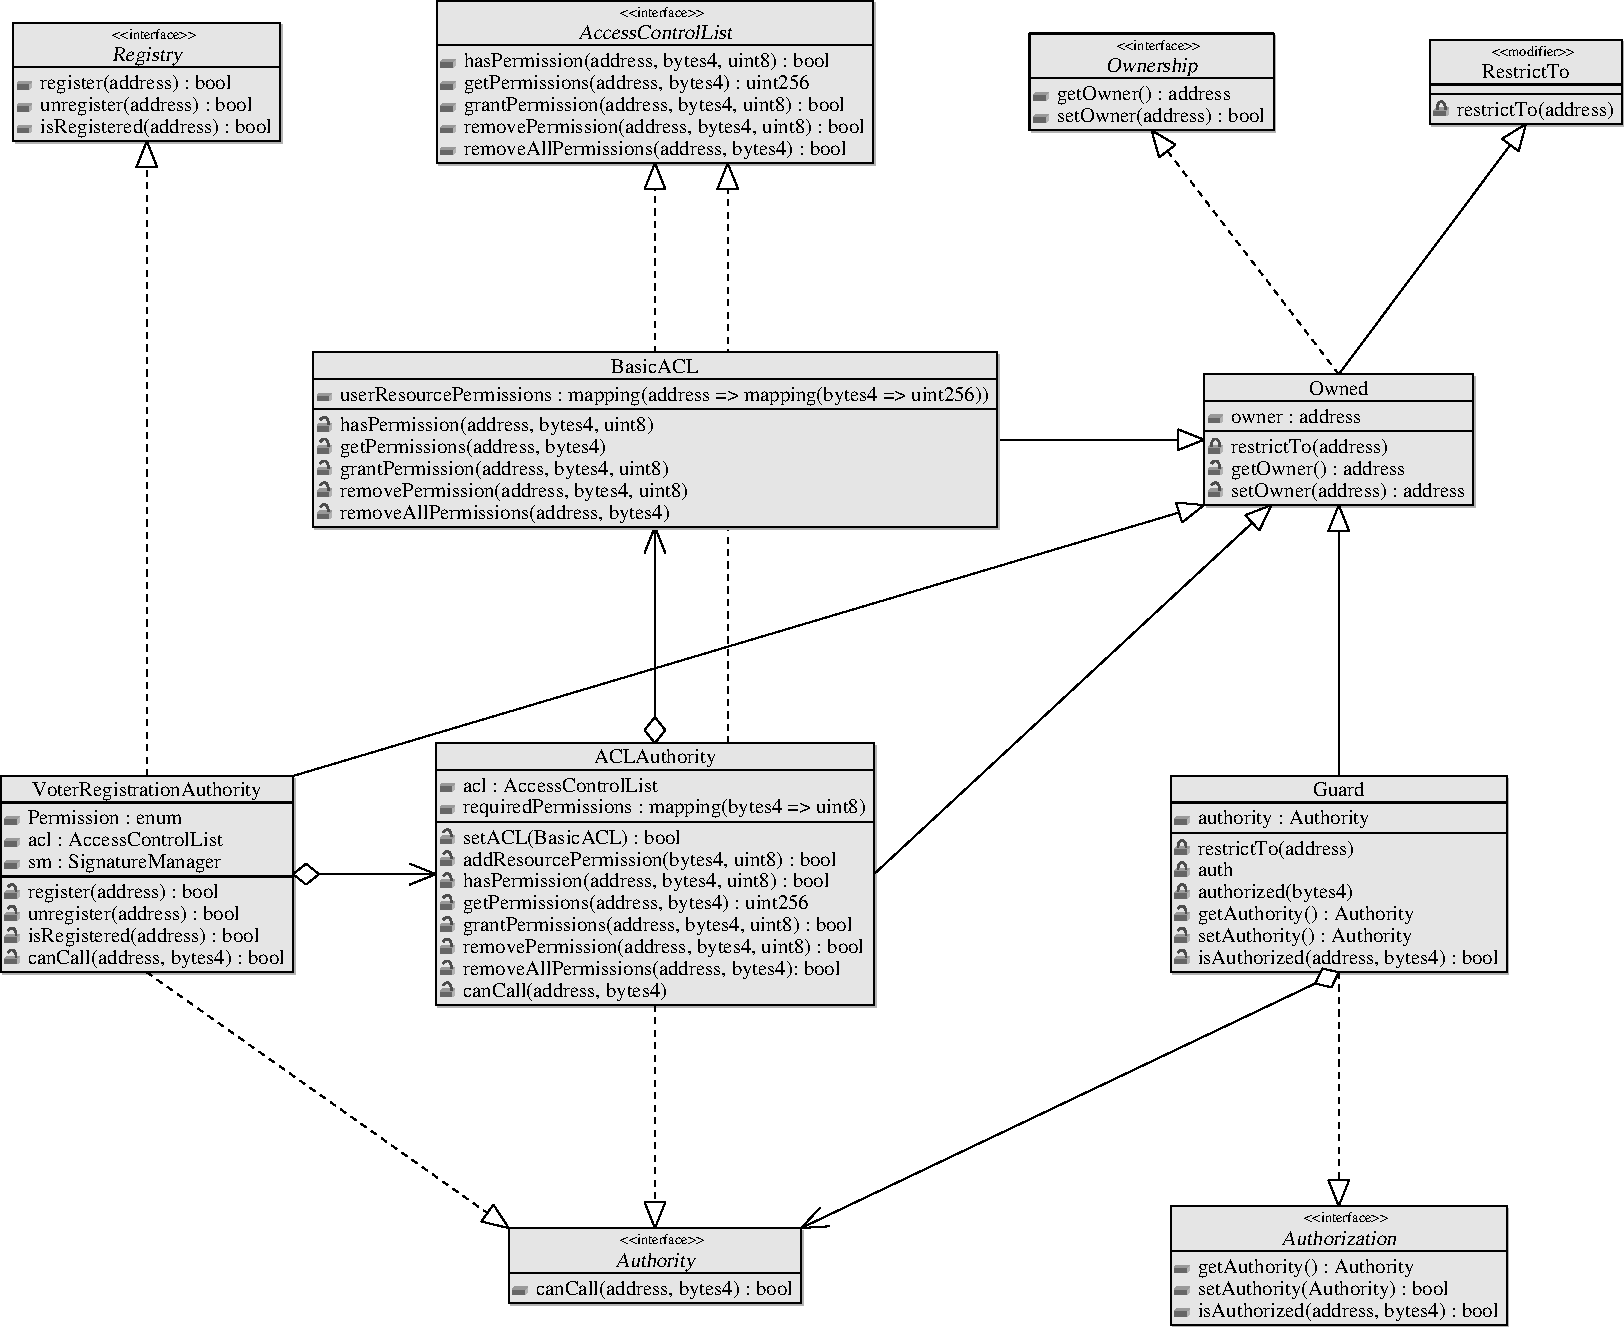
\includegraphics[width=\textwidth]{figures/authorization/figure}
  % \includestandalone[width=\textwidth]{\fig{authorization}}
\end{figure}

% Sub-sub-section: Managing Contract Ownership
\subsection{Primitive Contract Ownership}

Managing \solt{contract} ownership is one of the most basic forms of access
control in the Ethereum ecosystem. Here we introduce:

\begin{enumerate}
  \item \sol{interface Ownership}, which defines \solt{function}[s] to
    express \solt{contract} ownership,
  \item \sol{contract RestrictTo}, which defines a \solt{modifier} for
    restricting access to \solt{function} calls based on an \solt{address}, and
  \item \sol{contract Owned}, a convenience \solt{contract}, which provides an
    implementation of \sol{interface Ownership} and leverages
    \sol{contract RestrictTo}.
\end{enumerate}

\begin{figure}[H]
  \centering
  \caption{Contract ownership dependency graph modeling.}\label{fig:ownership}
  \figurepdf[]{ownership}
\end{figure}

\input{05-results/sections/authorization/contract-restrictto}

\input{05-results/sections/authorization/interface-ownership}

\input{05-results/sections/authorization/contract-owned}

% Sub-sub-section: Generalizing Contract Access Control
\subsection{Generalizing Contract Access Control}

In order to generalize \solt{contract} access control we introduce:

\begin{enumerate}
  \item \sol{interface Authority}, which defines \solt{function}[s] to determine
    whether some \emph{subject} is permitted to access some \emph{resource},
  \item \sol{contract Authorization}, which defines a \solt{modifier} for
    restricting access to \solt{function} calls based on an \solt{address}, and
  \item \sol{contract Guard}, a convenience \solt{contract}, which provides an
    implementation of \sol{interface Authorization} by aggregating
    implementations of \sol{interface Authority}.
\end{enumerate}

Together these components allow us to provide a generalized access control
model; isolating and deferring the responsibilities of
authorization.\footnotemark{}
\todo{Alternative names: Guard, Authority, Enforcer, Authorization}

\footnotetext{
  I think I would maybe prefer \sol{interface Authorization} to define
  \sol{isAuthorized} and for \sol{interface Authority} to define
  \sol{getAuthority} and \sol{setAuthority}.

  A better name in that case might be \sol{interface AuthorityManager}.
}

\begin{figure}[H]
  \centering
  \caption{Generalized contract access control.}% \label{fig:authorization}
  \figurepdf[]{guard}
  % 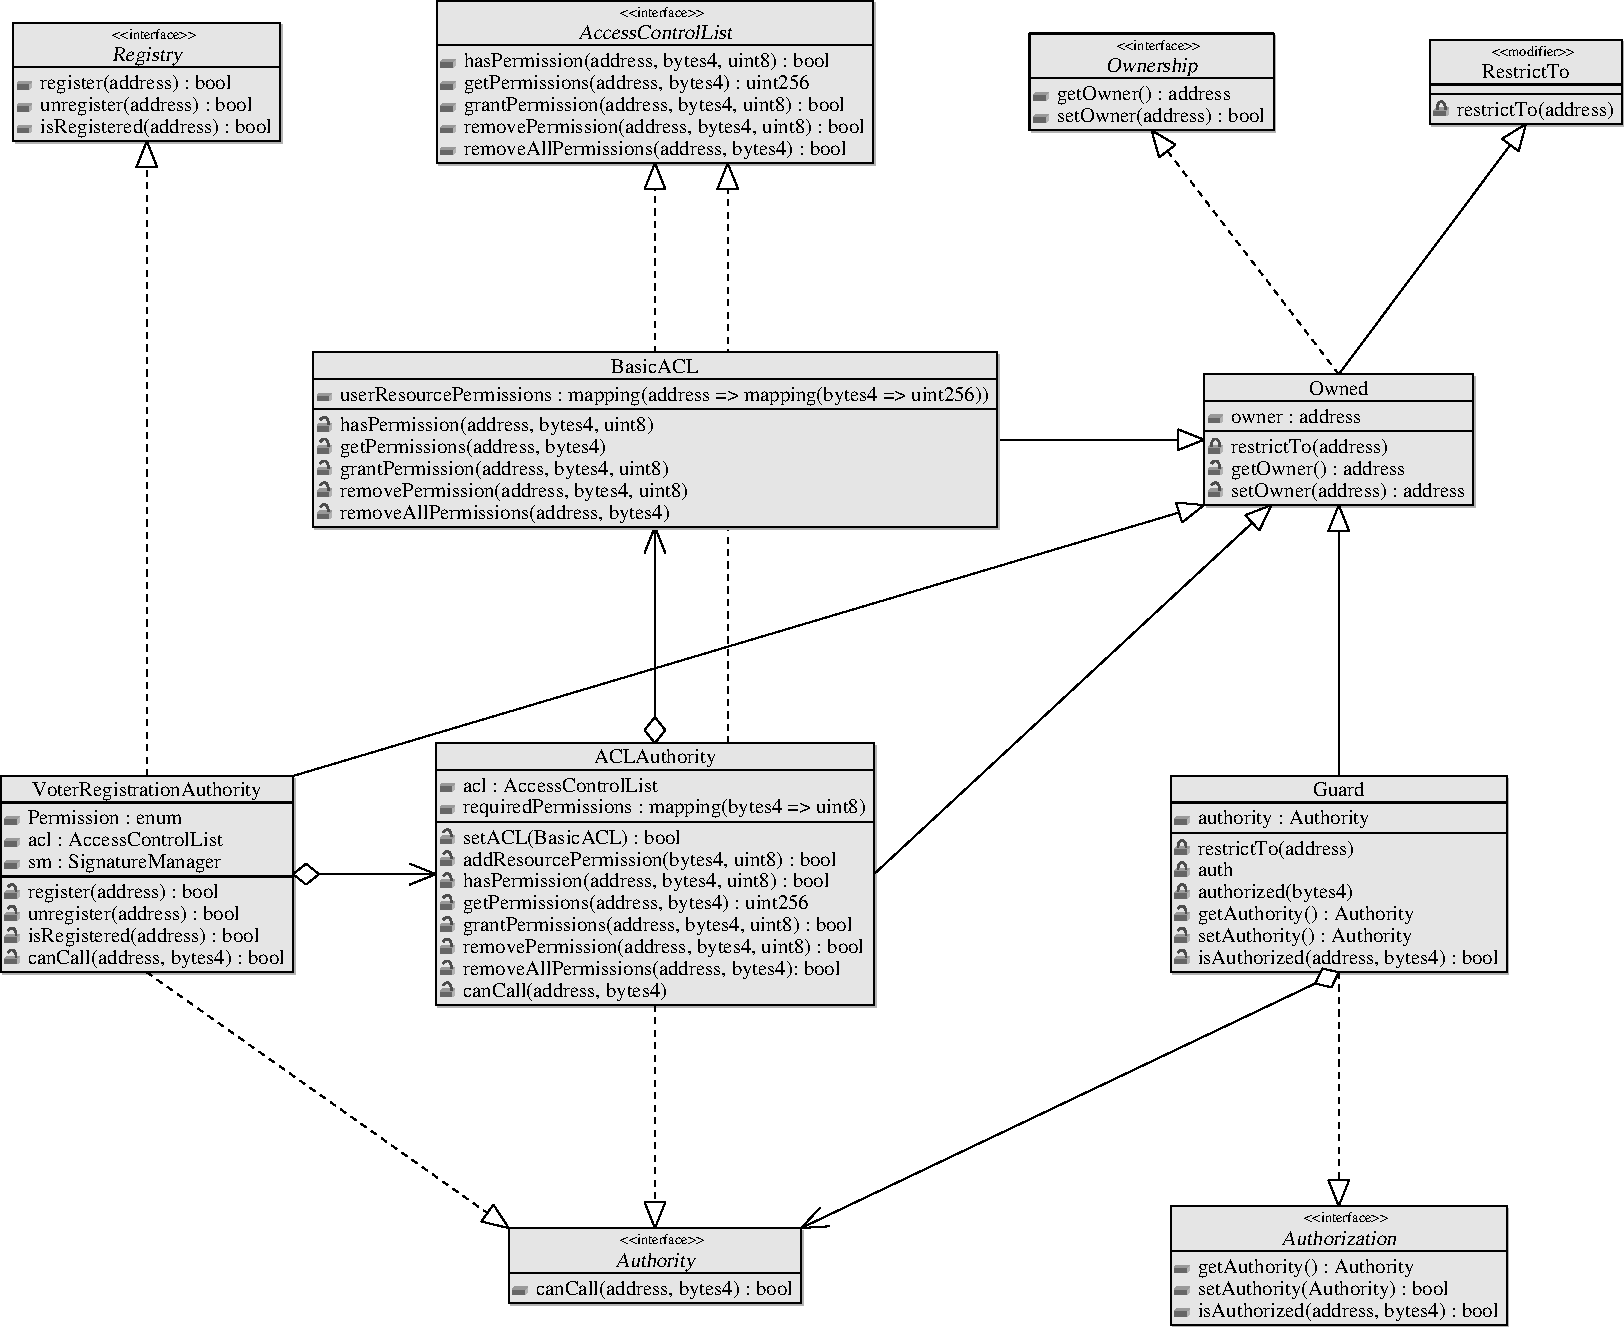
\includegraphics[width=\textwidth]{figures/authorization/figure}
  % \includestandalone[width=\textwidth]{\fig{authorization}}
\end{figure}

\input{05-results/sections/authorization/interface-authority}

\input{05-results/sections/authorization/interface-authorization}

\input{05-results/sections/authorization/contract-guard}

% Sub-sub-section: Access Control Lists
\subsection{Access Control Lists}

We introduce access control lists to provide a generalized form of access
control through a well-understood and common interface:

\begin{enumerate}
  \item \sol{interface AccessControlList}, which defines the basic actions
    required for an access control list implementation;

  \item \sol{contract BasicACL}, which provides a basic implementation of
    \sol{interface AccessControlList}; and

  \item \sol{contract ACLAuthority}, which aggregates an
    \solt{interface AccessControlList} implementation, \sol{contract BasicACL}
    in this case, to back an \sol{interface Authority} implementation.
\end{enumerate}

\begin{figure}[H]
  \centering
  \caption{Generalized contract access control by way of access control lists.}\label{fig:acl}
  \figurepdf[]{access-control-lists}
  % 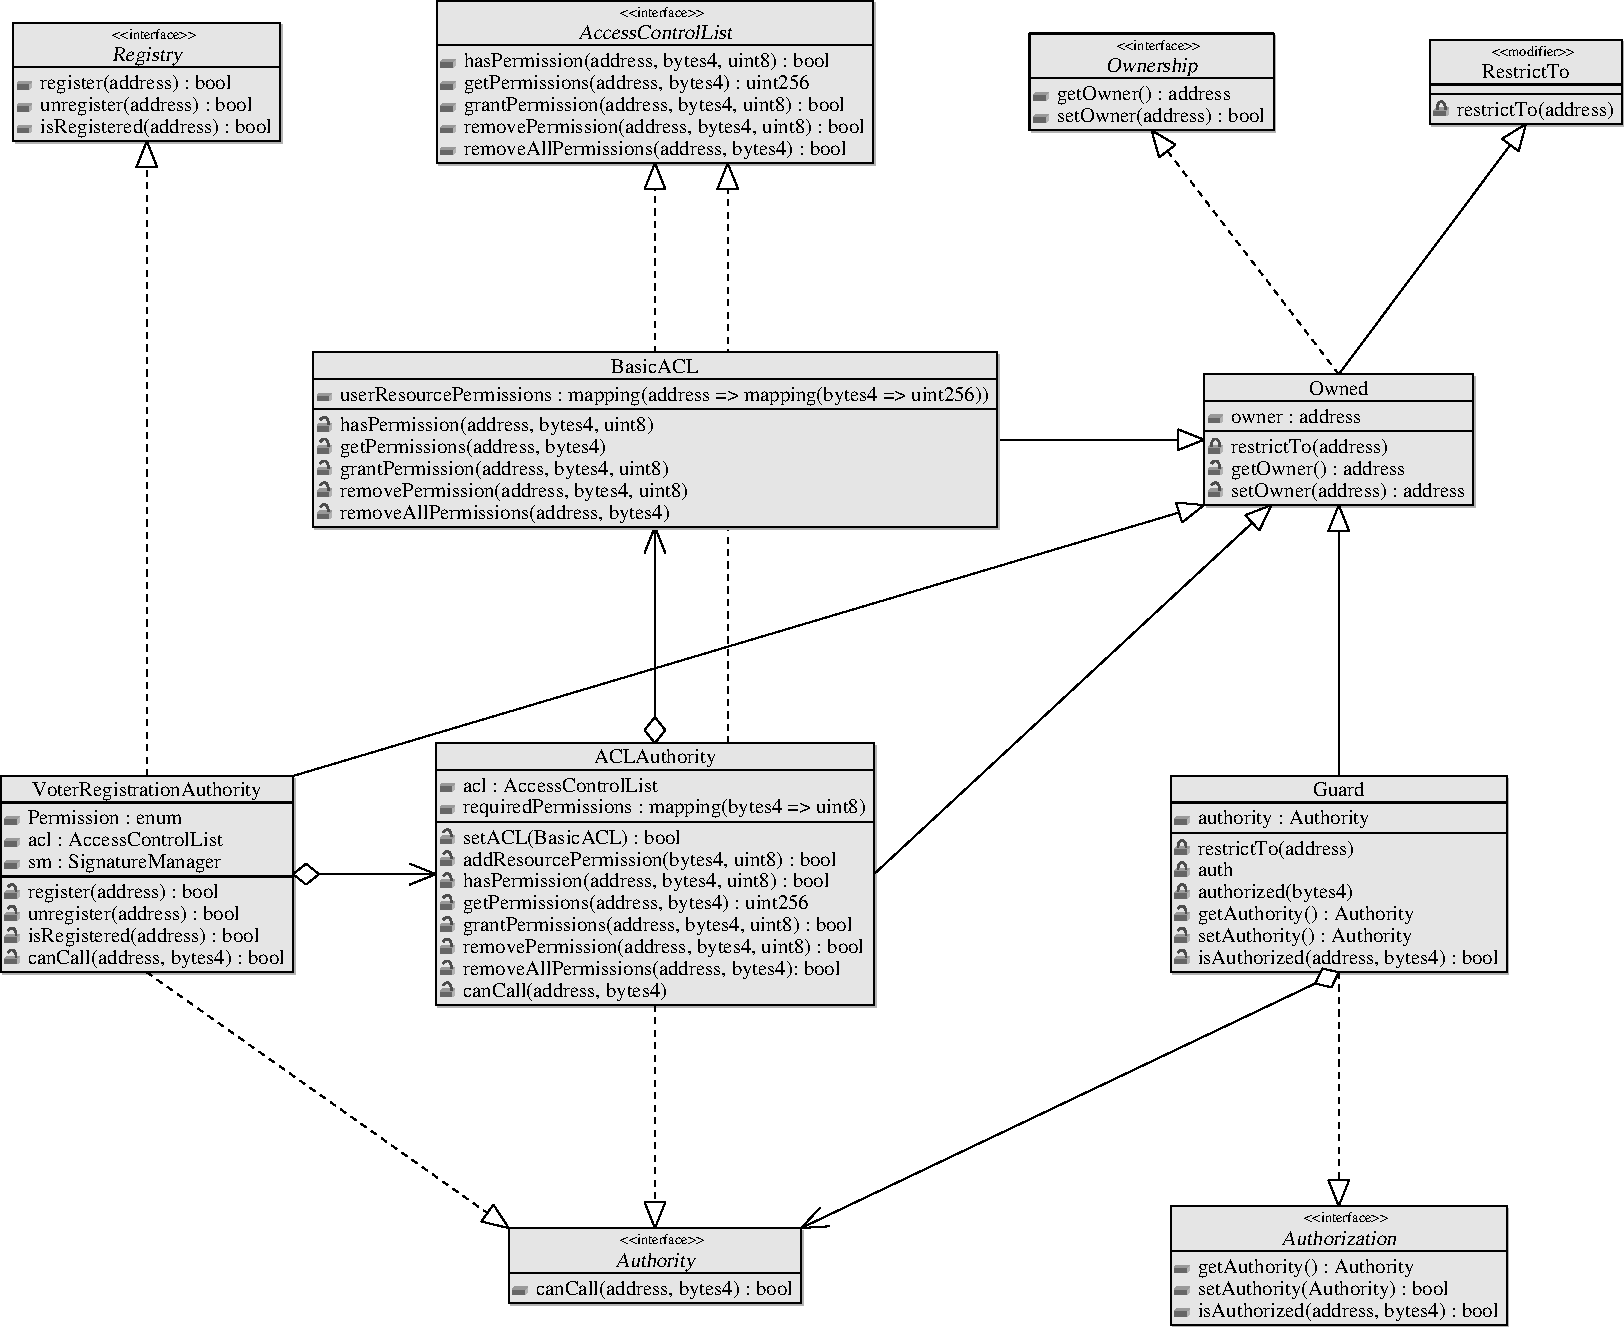
\includegraphics[width=\textwidth]{figures/authorization/figure}
  % \includestandalone[width=\textwidth]{\fig{authorization}}
\end{figure}

\input{05-results/sections/authorization/interface-acl}

\input{05-results/sections/authorization/contract-basic-acl}

\input{05-results/sections/authorization/contract-acl-authority}

% Sub-sub-section: Registries
\subsection{Registries}

Having completed the work of generalizing access control and building access
control lists, we now introduce a simplified access control model for managing
voter registration during elections.

\begin{enumerate}
  \item \sol{interface Registry}, which defines the functions for registering
    voters for an election, and
  \item \sol{contract VoterRegistrationAuthority}, which implements and
    aggregates several \solt{interface}[s] and \solt{interface} implementations
    --- namely \sol{interface Registry}, \sol{interface Authority}, and
    \sol{contract ACLAuthority} --- to build a trusted source of registered
    voters.
\end{enumerate}

\begin{figure}[H]
  \centering
  \caption{Simplified election registry.}\label{fig:registry}
  \figurepdf[]{registry}
  % 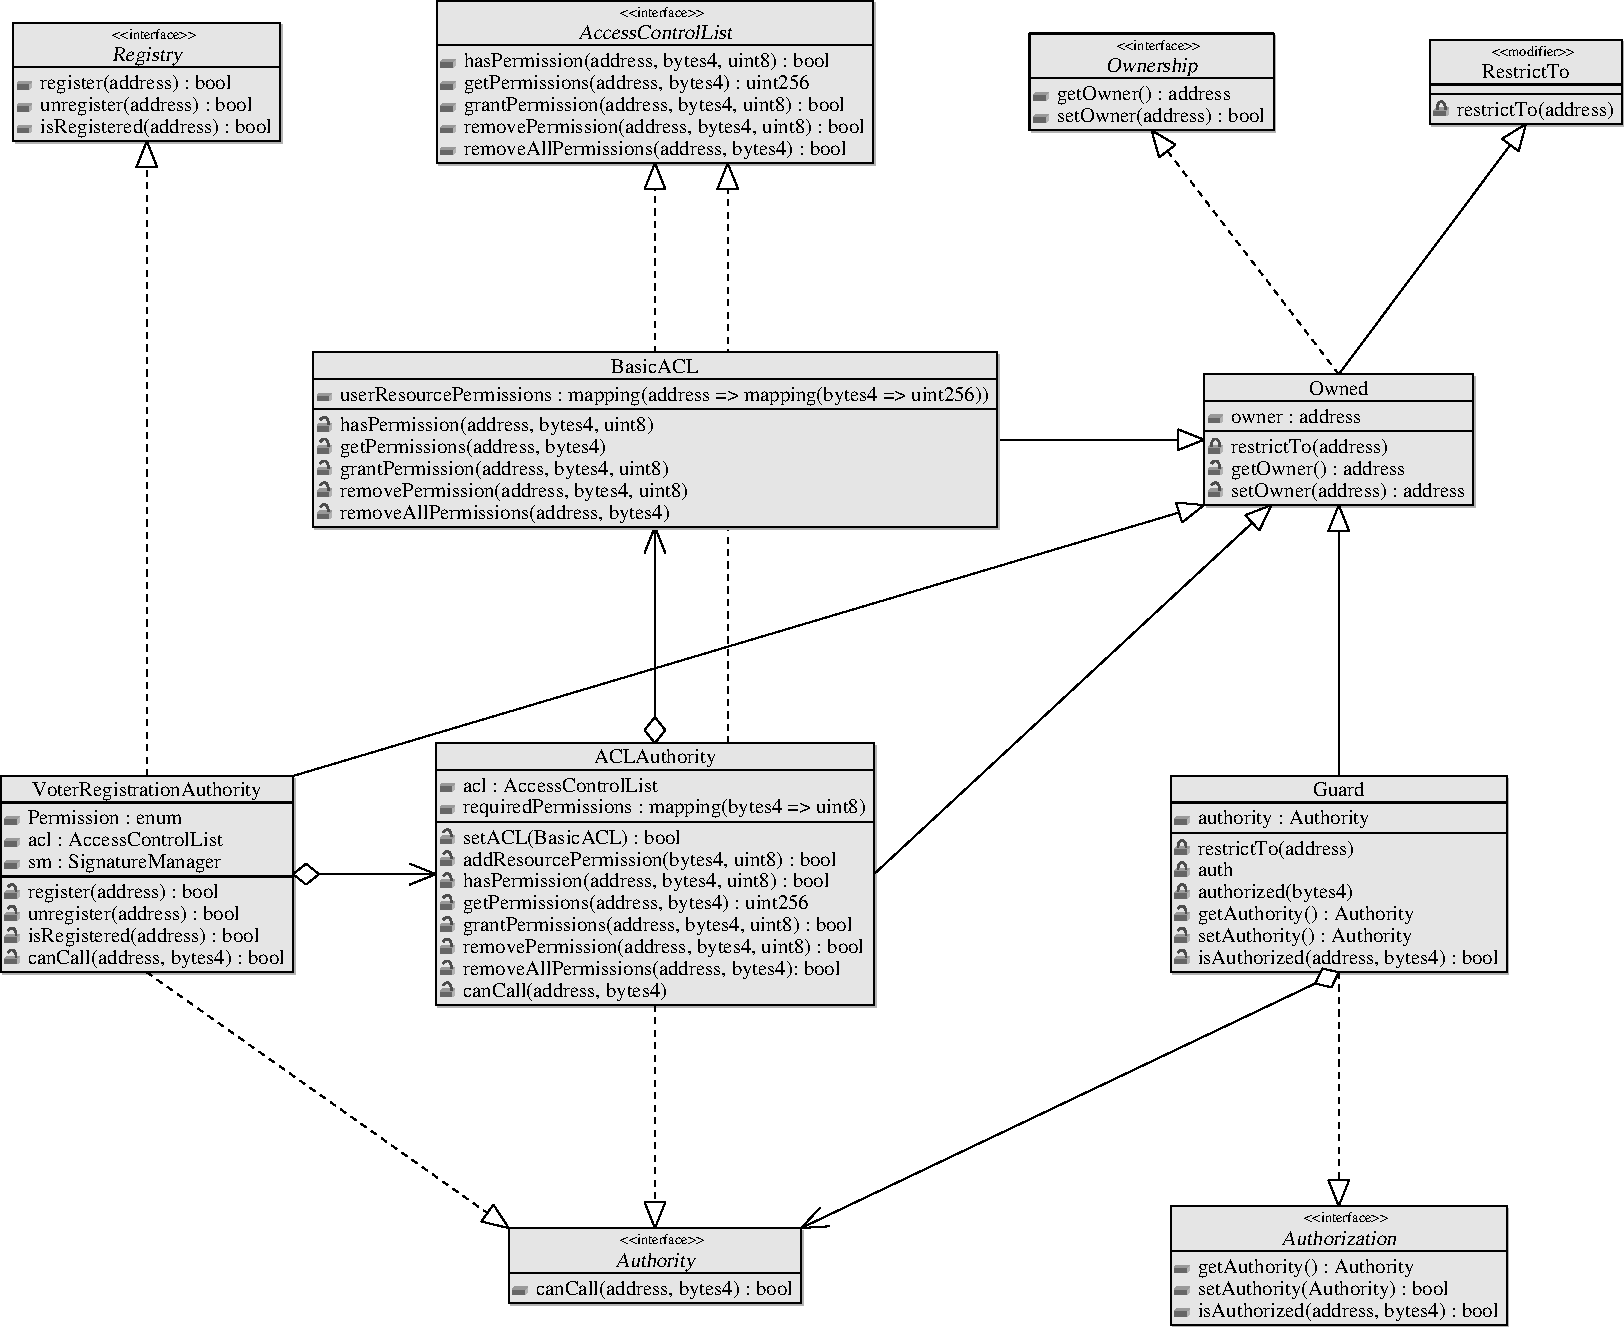
\includegraphics[width=\textwidth]{figures/authorization/figure}
  % \includestandalone[width=\textwidth]{\fig{authorization}}
\end{figure}

\input{05-results/sections/authorization/interface-registry}

\input{05-results/sections/authorization/contract-voter-registration-authority}


% Section: Election Components
% \section{Election Components}

This section explores the components relating to elections; election contracts:

\begin{enumerate}
  \item \emph{First-Past-the-Post},
  \item \emph{Range Vote}, and
  \item \emph{Single Transferable Vote}.
\end{enumerate}

% \begin{figure}[H]
%   \centering
%   \caption{Authorization dependency graph modeling.}% \label{fig:authorization}
%   \figurepdf[width=\textwidth]{authorization}
%   % 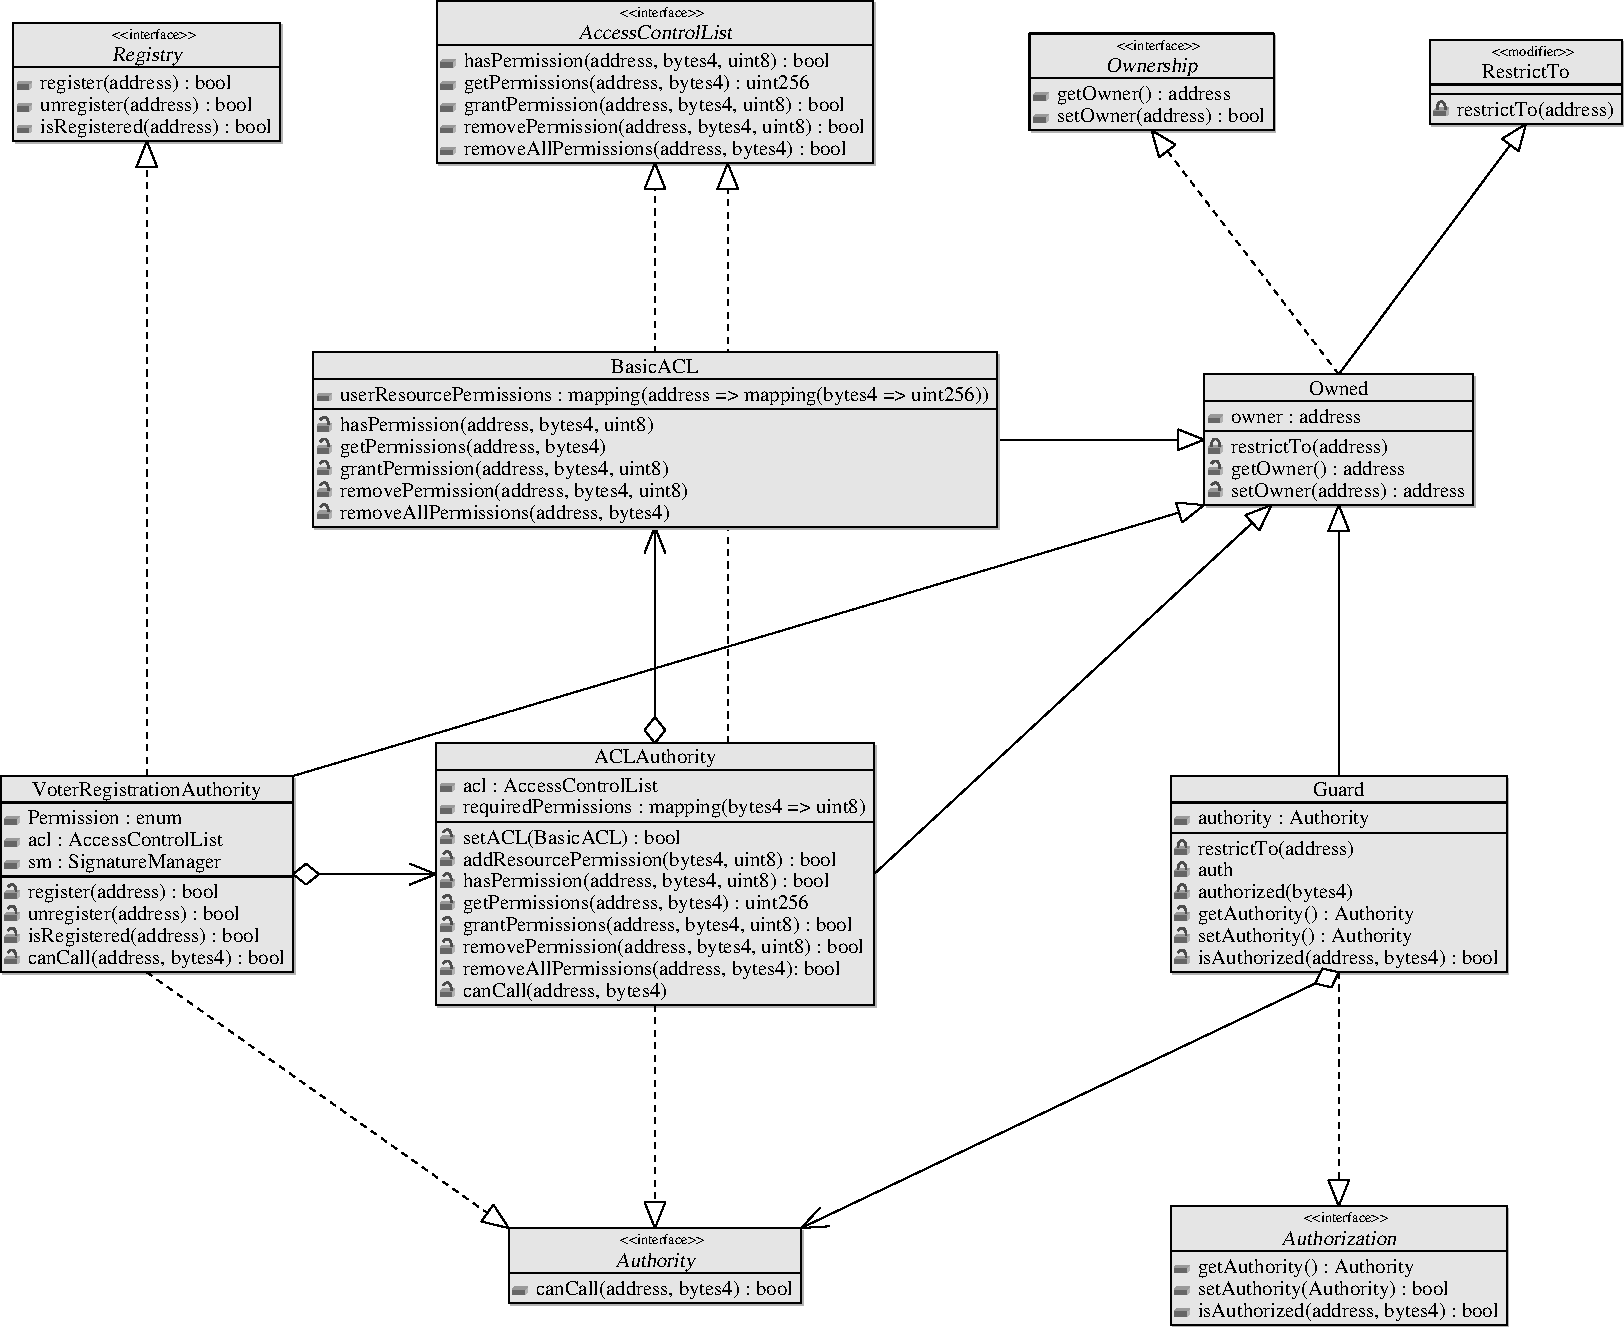
\includegraphics[width=\textwidth]{figures/authorization/figure}
%   % \includestandalone[width=\textwidth]{\fig{authorization}}
% \end{figure}

% \subsection{Finite State Machine}

% \subsection{First-Past-the-Post}
% The first-past-the-post \solt{contract} is the simplest election \solt{contract}
% implementation.

\subsection{Election Contracts}

\input{05-results/sections/election/first-past-the-post}

\subsubsection{Range Vote}

\subsubsection{Single Transferable Vote}


% Section: Delegation Components
% \section{Delegation Components}

This section explores the components relating to vote delegation. The delegation
components are responsible for managing the delegation of voters' votes to
delegates.

% \begin{figure}[H]
%   \centering
%   \caption{Authorization dependency graph modeling.}% \label{fig:authorization}
%   \figurepdf[width=\textwidth]{authorization}
%   % 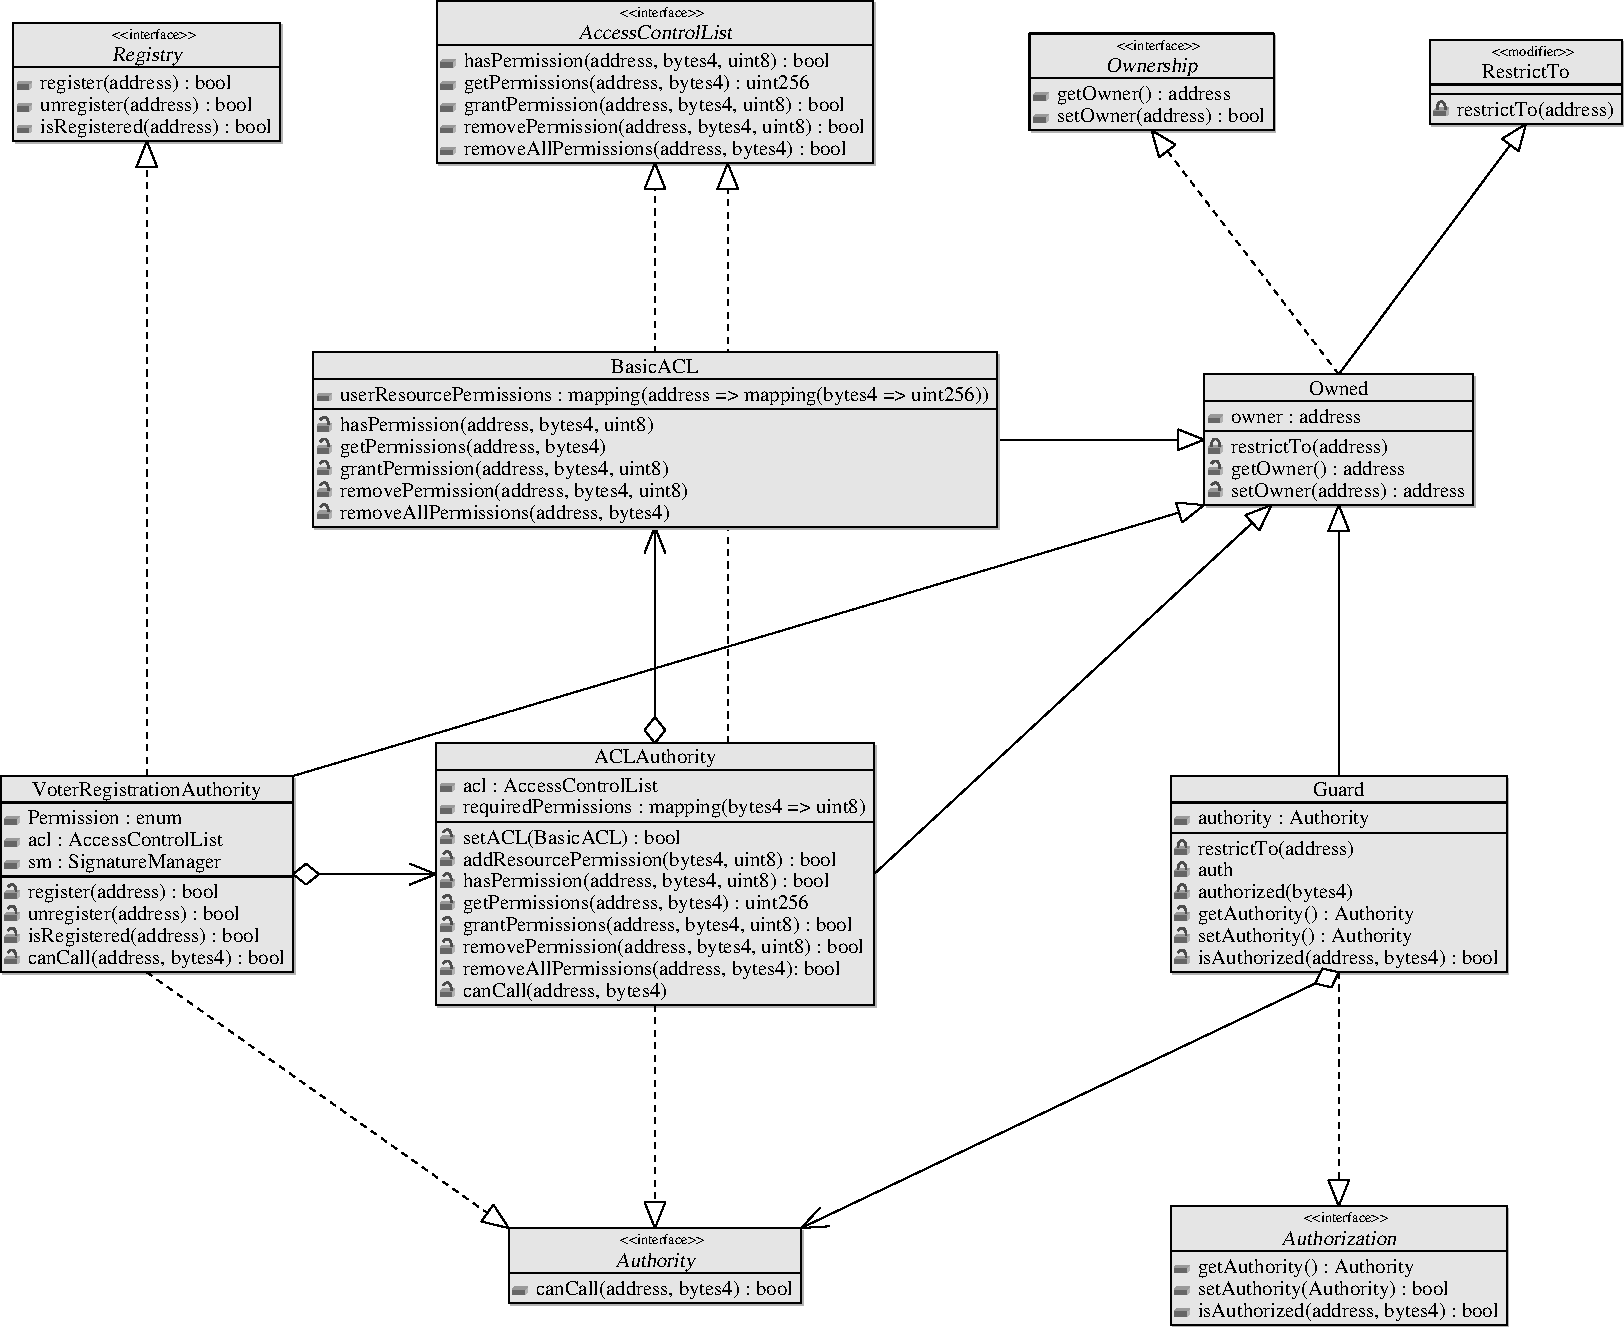
\includegraphics[width=\textwidth]{figures/authorization/figure}
%   % \includestandalone[width=\textwidth]{\fig{authorization}}
% \end{figure}

% Section: delegation
\input{05-results/sections/delegation/delegation}



% \chapter{Discussion}\label{chap:discussion}

\section{Contracts}
\subsection{Delegation Contract \& Registration Authority}
The delegation contract, and to some degree the registration authority, suffer
from issues with respect to state management, multi-contract usage, and
concurrency generally. It would be ideal (for conceptual, storage, and
computational reasons) for multiple contracts to leverage the same registration
authority and delegation contracts. Unfortunately issues begin to arise as
electoral contracts in different phases begin querying the registration
authorities and delegation contracts. This is further complicated as malicious
actors attempt to subvert the electoral system.

To begin to understand the issue we can imagine a single FPTP election contract
\lstinline|A| which is leveraging a delegation contract \lstinline|D|. The FPTP
contract \lstinline|A| expects delegation changes to continue until it enters
its \lstinline|Tally| phase, at which point it should expect the delegation
contract to enter a read-only or write-blocking mode. This might occur through
some mutex mechanism. This locking mechanism is necessary because the FPTP
election contract must accurately determine the weight of each vote for each
delegate. If the delegation contract is not locked a delegate might transfer his
voting power to another delegate immediately after the FPTP election contract
\lstinline|A| determines his weight from delegation contract \lstinline|D| and
sums the delegate's votes to the total. The following example demonstrates this
issue:

\begin{enumerate}
    \item Voting Begins
    \begin{enumerate}[i.]
        \item Delegate X with a voting weight of 5 casts a ballot for choice A.
        \item Delegate Y with a voting weight of 1 casts a ballot for choice A.
        \item Delegate Z with a voting weight of 10 casts a ballot for choice B.
    \end{enumerate}
    \item Voting Ends
    \item Tallying Begins
    \begin{enumerate}[i.]
        \item The election contract sums delegate X's $vote*weight$ to choice A.
            Choice A now has 5 votes in its favor.
        \item Delegate X confers his votes to delegate Y. Y now has a weight of
            6 votes.
        \item The election contract sums delegate Y's $vote*weight$ to choice A.
            Choice A now has 11 votes in its favor.
        \item The election contract sums delegate Z's $vote*weight$ to choice B.
            Choice B now has 10 votes in its favor.
    \end{enumerate}
    \item Tallying Ends
    \begin{enumerate}[i.]
        \item Choice A wins by 1 vote (11 to 10) despite only having 6 votes
            cast in its favor.
    \end{enumerate}
\end{enumerate}

It is clear that \lstinline|B| should have won this contest 10 to 6. This
failure to properly tally the results is a product of the classic
readers-writers concurrency problem and represents a clear danger to any
electoral system. A common solution to the readers-writers problem is to
implement a simple mutex mechanism. For example, we could in the delegation
contract allow readers to lock writing to the delegation contract until the
readers have finished reading from the contract.  This is known as the
readers-preference solution. A simple improvement beyond that might be to cache
delegations in a separate data structure as a sort of journaling system while
the delegation contract is locked. These delegations could be combined and
applied as a single commit to the contract state as soon as the contract is
unlocked, this is the writers-preference solution. In this way the electorate
could still confer their votes freely to their delegates and have those
delegations reflected in the next election or tally.

This works well under some circumstances; e.g., when a small set of electoral
contracts interacting with a delegation contract non-maliciously; however, if
ever a malicious or broken electoral contract failed to release the lock, then
the writers would starve, essentially preventing the electorate from ever
conferring their votes to a delegate again.

We can imagine solving this starvation issue by giving the delegation contract
the ability to take back a mutex after a specified period of time, however, if
the electoral contract was not malfunctioning or malicious and simply performing
a long-running tally of votes then it's very likely that the voting actors would
have either maliciously or accidentally corrupted the tally results once the
delegation contract unlocked itself to commit its journaled delegations.

Further, even if we imagined a perfectly functional electoral contract with a
short tally process, issues still manifest themselves as multiple instances of
that electoral contract begin to request the delegation contract be locked.
There's a chance that the writers become starved if in a reader-preference
solution. This is not so serious a concern in a writer-preference solution where
mutexes expire, but a much larger concern then appears, which is that a
writers-preference solution would produce an ever-expanding queue of electoral
contracts depending on the delegation contract. This occurs because readers
would be forced to operate serially to prevent their election contract state
from becoming corrupted by trying to begin a read/tally process in the middle or
late stages of another election contract's read/tally process. This is clearly
suboptimal.

The solution to this problem would likely involve the electoral contract being
able to specify the root of the delegation contract's Merkle DAG state; this
would functionally act as a fingerprint of the state of the delegation contract
which the election contract wishes to operate against. This concept is not too
dissimilar from git commits. Unfortunately the EVM does not currently offer such
functionality.  There are several mechanisms which, if offered by Ethereum's
EVM, would support such functionality. One mechanism to support this
functionality would be via explicit contract state checkpoints, however, this
would likely be a prohibitively expensive operation for storage reasons. Another
mechanism would be to support invertible operation definitions, thus allowing a
node to rewind the state of a contract. Such functionality would only be
computationally expensive, but potentially prohibitively so if there had been
many state modifications since the commit a contract wishes to operate against.
A combination of these two mechanisms might offer the best solution.

\section{Performance}


\section{Voter Registration List Population}



\subsection{Design Principles}
We borrow design principles from ``Electoral System Design: The New
International IDEA Handbook'' which were outlined in Chapters 2 and 3.

\subparagraph{Representation} We wish to achieve fair representation. What
constitutes fair representation will largely depend on the greater democratic
framework and the constitutes of that framework. Our electoral system should
translate votes into winning choices in a way that accurately and fairly
represents the will of the people while also being flexible enough to allow for
configuration and modification appropriate for various governance structures.

\subparagraph{Transparency} Our electoral system should be as transparent as
possible, preferably end-to-end verifiable. The winners, losers, and electorate
must be able to trust that the results of an election were achieved
legitimately.

\subparagraph{Inclusiveness} Our electoral system should support full suffrage
(active and passive) as well as universal suffrage. The mechanisms of the
electoral system should not be biased such that any group is discriminated
against. Designing an electoral system with inclusiveness in mind results in
governance with a stronger sense of legitimacy and wider participation and
willingness to participate by the electorate.

\paragraph{International Standards} There is no universally agreed upon
standards, but most would agree upon the following standards.

\begin{enumerate}[label=\Large$\square$]
  \item Elections should be free, fair, and periodic.
  \item Universal adult suffrage should be supported.
  \item Ballot secrecy should be preserved and constituents should be free
    from coercion.
  \item A commitment to the principle of ``one person, one vote.''
\end{enumerate}

\paragraph{Design Checklist}
We also borrow a design checklist from the ``Electoral System Design: The New
International IDEA Handbook.''
\todo{This should be moved to the conclusion.}

\begin{enumerate}[label=\Large$\square$]
  \item Is the system clear and comprehensible?
  \item Has context been taken into account?
  \item Is the system appropriate for the time?
  \item Are the mechanisms for future reform clear?
  \item Does the system avoid underestimating the electorate?
  \item Is the system as inclusive as possible?
  \item Was the design process perceived to be legitimate?
  \item Will the election results be seen as legitimate?
  \item Are unusual contingencies taken into account?
  \item Is the system financially and administratively sustainable?
  \item Will the voters feel motivated to participate?
  \item Is a competitive party system encouraged?
  \item Does the system fit into a holistic constitutional framework?
  \item Will the system help alleviate conflict rather than exacerbate it?
\end{enumerate}

\chapter{Conclusion}\label{chap:conclusion}

The issues faced by governments and societies --- especially while wrestling
with issues such as the COVID-19 pandemic, state-sponsored election
interference, and claims of election fraud --- demonstrate a clear need for
improvements with regards to electoral systems, voting systems, and governance
models. The concept of decentralized organizations, democratically operating and
existing on-chain, offers a provocative and alluring alternative approach which
might have the potential to support more egalitarian and meritocratic social
structures and governance models. Section~\ref{sec:elections} introduced
elections, electoral systems, and the tools available for analyzing them.
Section~\ref{sec:blockchain-technologies} introduced blockchain technologies,
their design, and the properties thereof which might prove useful in a number of
systems, such as voting, where a high degree of verifiability and confidence of
correctness is required.

The literature reviewed in Section~\ref{sec:internet-voting} demonstrates the
difficulty of building Internet-based voting systems, and reviews a number of
theoretical and real-world attacks that have been demonstrated in the various
attempts to build such systems. As seen in Section~\ref{sec:e2e-viv}, the
tensions present in the security, privacy, and authentication requirements of
voting systems are challenging to resolve; however, although still not without
risks, there is promise in Internet voting if systems can be designed which
achieve end-to-end verifiability.

Section~\ref{sec:architecture-and-design} explored several election,
authorization, and delegation designs for use on the Ethereum blockchain.
However, although Chapter~\ref{chap:results} demonstrated the possibility
implementing such systems, the issues outlined in Section~\ref{sec:analysis}
make clear that the Ethereum blockchain still requires many improvements before
it could be considered capable of supporting the kind of next-generation
elections and electoral systems this research sought to investigate.

Among other things, the semantics available for building such systems are
complex and unintuitive, an inevitable source of bugs. Further, tools and
techniques, which are currently unavailable, are necessary to support
large-scale systems such as voting; for example, inter-contract communication
and inter-block computations should be possible with consistent states available
across contract boundaries from start to end of computation.

More importantly, the computation and storage requirements demanded for
electoral system operation is too high to make their use on-chain practical in
most scenarios. Measuring generously, the least expensive vote operation listed
in Table~\ref{tab:election-simulations} would cost the equivalent of \$7.87, the
average of these vote operations (across electoral systems implementations)
measures in at \$28.18 per vote, and in the worst case a single vote operation
might cost upwards of \$57.11. The cost of executing the most-expensive tallying
operation is significantly worse, costing the equivalent of over \$1,300.00 to
tally the ballots of an election simulation with just 100 voters.\footnotemark{}
These prices are clearly far too high for serious consideration, and at best
they exclude from consideration a large number of popular electoral systems
which have much higher computation and storage demands than the ones selected.

\footnotetext{The gas price at the time of writing is approximately 120 gwei.}

These costs appear even worse when viewed in light of the fact that the
measurements made in Table~\ref{tab:election-simulations} were the product of
electoral system implementations which were specifically designed to accurately
measure the raw costs of the electoral systems' computational and storage
requirements, and therefore included no security or state management systems
beyond that. Inclusion of such systems which would certainly have made these
operations more costly. Still, these results should not be viewed in vacuum;
some estimates put the cost of election administration in the US at around
\$8.00 per voter, so the lower bounds of these results suggest that there is
potential here, especially with advancements to the Ethereum network and if some
scaling issues can be resolved.

\section*{Summary of Accomplishments}

\begin{itemize}
  \item Designed authorization components for managing voter registration and
    providing access control in a generalized way.

  \item Implemented election contracts, tests, and simulations to benchmark and
    analyze electoral system performance and cost.

  \item Identified electoral system criteria relevant to Ethereum-based
    implementations of electoral systems.

  \item Identified techniques for improving some performance characteristics
    of electoral systems.

  \item Identified features which damage performance characteristics of
    electoral systems.
\end{itemize}

\section*{Future Work}

\begin{itemize}
  \item Unless scaling issues are resolved, it is likely that more reasonable
    approaches to on-chain electoral system design would involve using dedicated
    or permissioned blockchain implementations and leveraging the more
    traditional approaches to E2E-VIV security as outlined in
    Section~\ref{sec:e2e-viv} and Section~\ref{sec:analysis}.

  \item If scaling issues are resolved then the following items seem like
    worthwhile areas of research:

    \begin{itemize}
      \item A set of hardened electoral system contracts and libraries.

      \item Electoral system contracts which provide support for multi-winner
        elections and support proportional representation.

      \item A standardized election interface. This seems difficult to produce
        given the unique inputs and outputs required for different kinds of
        elections.

      \item An visual interface for marking and casting ballots to election
        contracts.

      \item Approaches and semantics for achieving consistency with
        inter-contract computation, especially with regards to inter-block
        computation.
    \end{itemize}
\end{itemize}

%==============================================================================

%-----------------------------------------------------------------------------%
% BIBLIOGRAPHY -- uncomment \nocite{*} to include items in 'mybib.bib' file
% that aren't cited in the text.  Change the style to match your
% discipline's standards.  Of course, if your bibliography file isn't called
% 'mybib.bib' you might want to change that here too :)
%-----------------------------------------------------------------------------%
\begin{spacing}{2}
  % Includes un-cited references in the bibliography from `.bib` files.
  \nocite{*}

  %%
  % natbib
  %%
  %% \bibliographystyle{humannat} %Formats bibliography
  % \bibliographystyle{bibliography/jasa} %Formats bibliography
  % \cleardoublepage{}
  % \normalbaselines{} %Fixes spacing of bibliography
  % \addcontentsline{toc}{chapter}{Bibliography} %adds Bibliography to your table of contents
  %% your bibliography file(s) - change the path if needed
  % \bibliography{
  %   bibliography/blockchain,
  %   bibliography/elections,
  %   bibliography/internet-voting
  % }

  %%
  % biblatex
  %%
  \printbibliography[heading=bibintoc]{}
  % \printbibliography[keyword={blockchain}, heading=bibintoc]{}
\end{spacing}

%-----------------------------------------------------------------------------%

%-----------------------------------------------------------------------------%
% APPENDICES -- OPTIONAL. These are just chapters enumerated by Appendix A,
%                Appendix B, Appendix C...
%-----------------------------------------------------------------------------%
\setstretch{2} % This should be \singlespacing
\begin{appendices}
  \chapter{Software Documentation}\label{appendix:documentation}

The source code, architecture, design, and documentation thereof of are
presented, reviewed, and provided here. The code reviewed in this section is not
guaranteed to represent the most accurate or recent state of the software and
is abbreviated throughout for readability. The most recent state of the
software can be found on GitHub.\cite{election-contracts} This appendix is
divided into three major sections:

\begin{itemize}
  \item \emph{Authorization Components}, which introduces the design and
    implementation of authorization-related components.

  \item \emph{Election Components}, which introduces the design and
    implementation of election-related components.

  \item \emph{Delegation Components}, which introduces the design and
    implementation of delegation-related components.
\end{itemize}


% Section: Authorization Components
\section{Authorization Components}

The authorization components are those which are responsible for managing access
control for \solt{contract}[s]. This section builds varying complexities of
access control beginning with:

\begin{enumerate}
  \item \emph{Primitive Contract Ownership}, which reviews basic access control
    mechanisms; then

  \item \emph{Generalized Access Control}, which introduces components for
    guarding access to resources; next

  \item \emph{Access Control Lists}, which demonstrate components for
    constructing and managing access control lists and integrating them with the
    components introduced for generalized access control; and finally,

  \item \emph{Registries}, which demonstrates voter registry components
    leveraging the aforementioned components to build and manage voter
    databases.
\end{enumerate}

\begin{figure}[H]
  \centering
  \figurepdf[width=\textwidth]{authorization}
  % 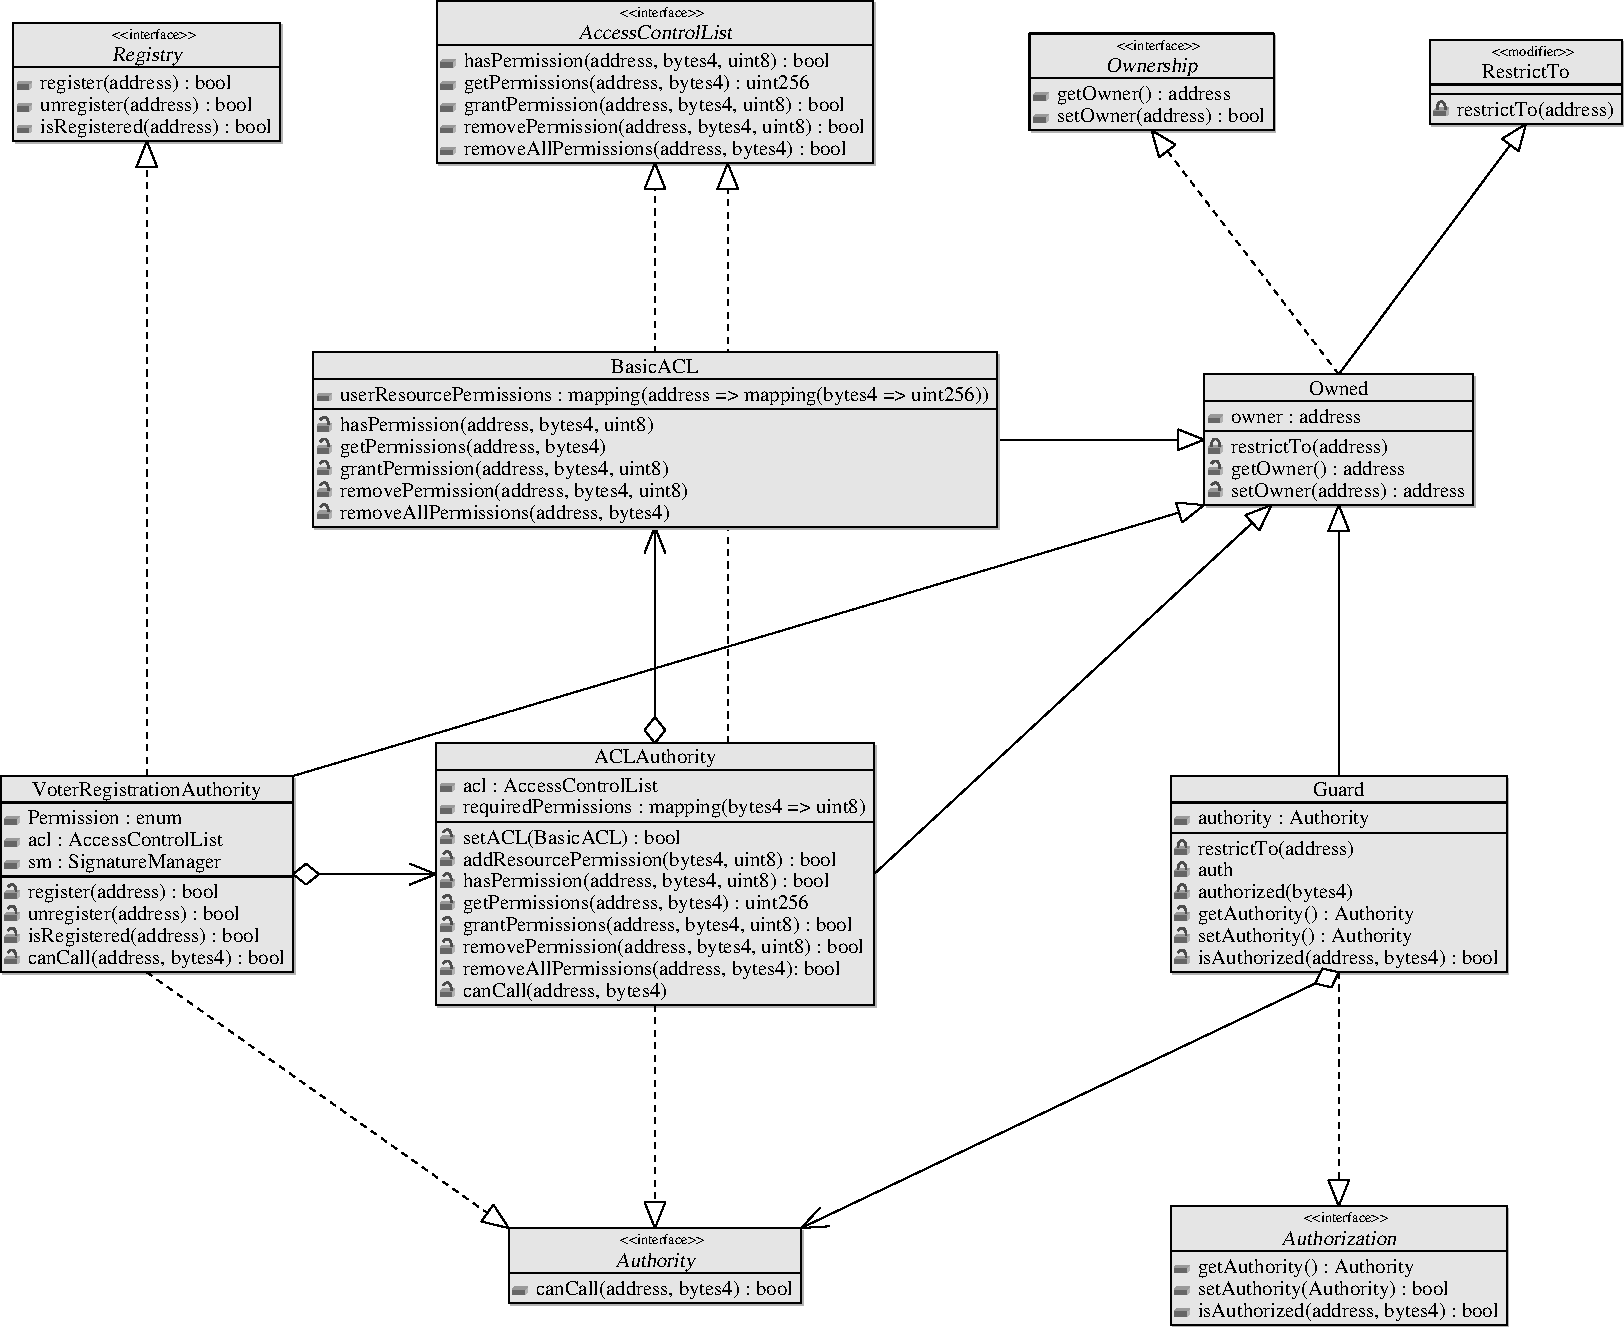
\includegraphics[width=\textwidth]{figures/authorization/figure}
  % \includestandalone[width=\textwidth]{\fig{authorization}}
  \caption{Authorization dependency graph modeling.}% \label{fig:authorization}
\end{figure}

% Sub-section: Managing Contract Ownership
\input{appendix/code/authorization/primitive-contract-ownership}

% Sub-section: Generalizing Contract Access Control
\input{appendix/code/authorization/generalizing-contract-access-control}

% Sub-section: Access Control Lists
\input{appendix/code/authorization/access-control-lists}

% Sub-section: Registries
\input{appendix/code/authorization/registries}


% Section: Election Components
\section{Election Components}

This section explores the components relating to elections.
% 
% \begin{enumerate}
%   \item \emph{First-Past-the-Post},
%   \item \emph{Range Vote}, and
%   \item \emph{Single Transferable Vote}.
% \end{enumerate}

% \begin{figure}[H]
%   \centering
%   \caption{Authorization dependency graph modeling.}% \label{fig:authorization}
%   \figurepdf[width=\textwidth]{authorization}
%   % 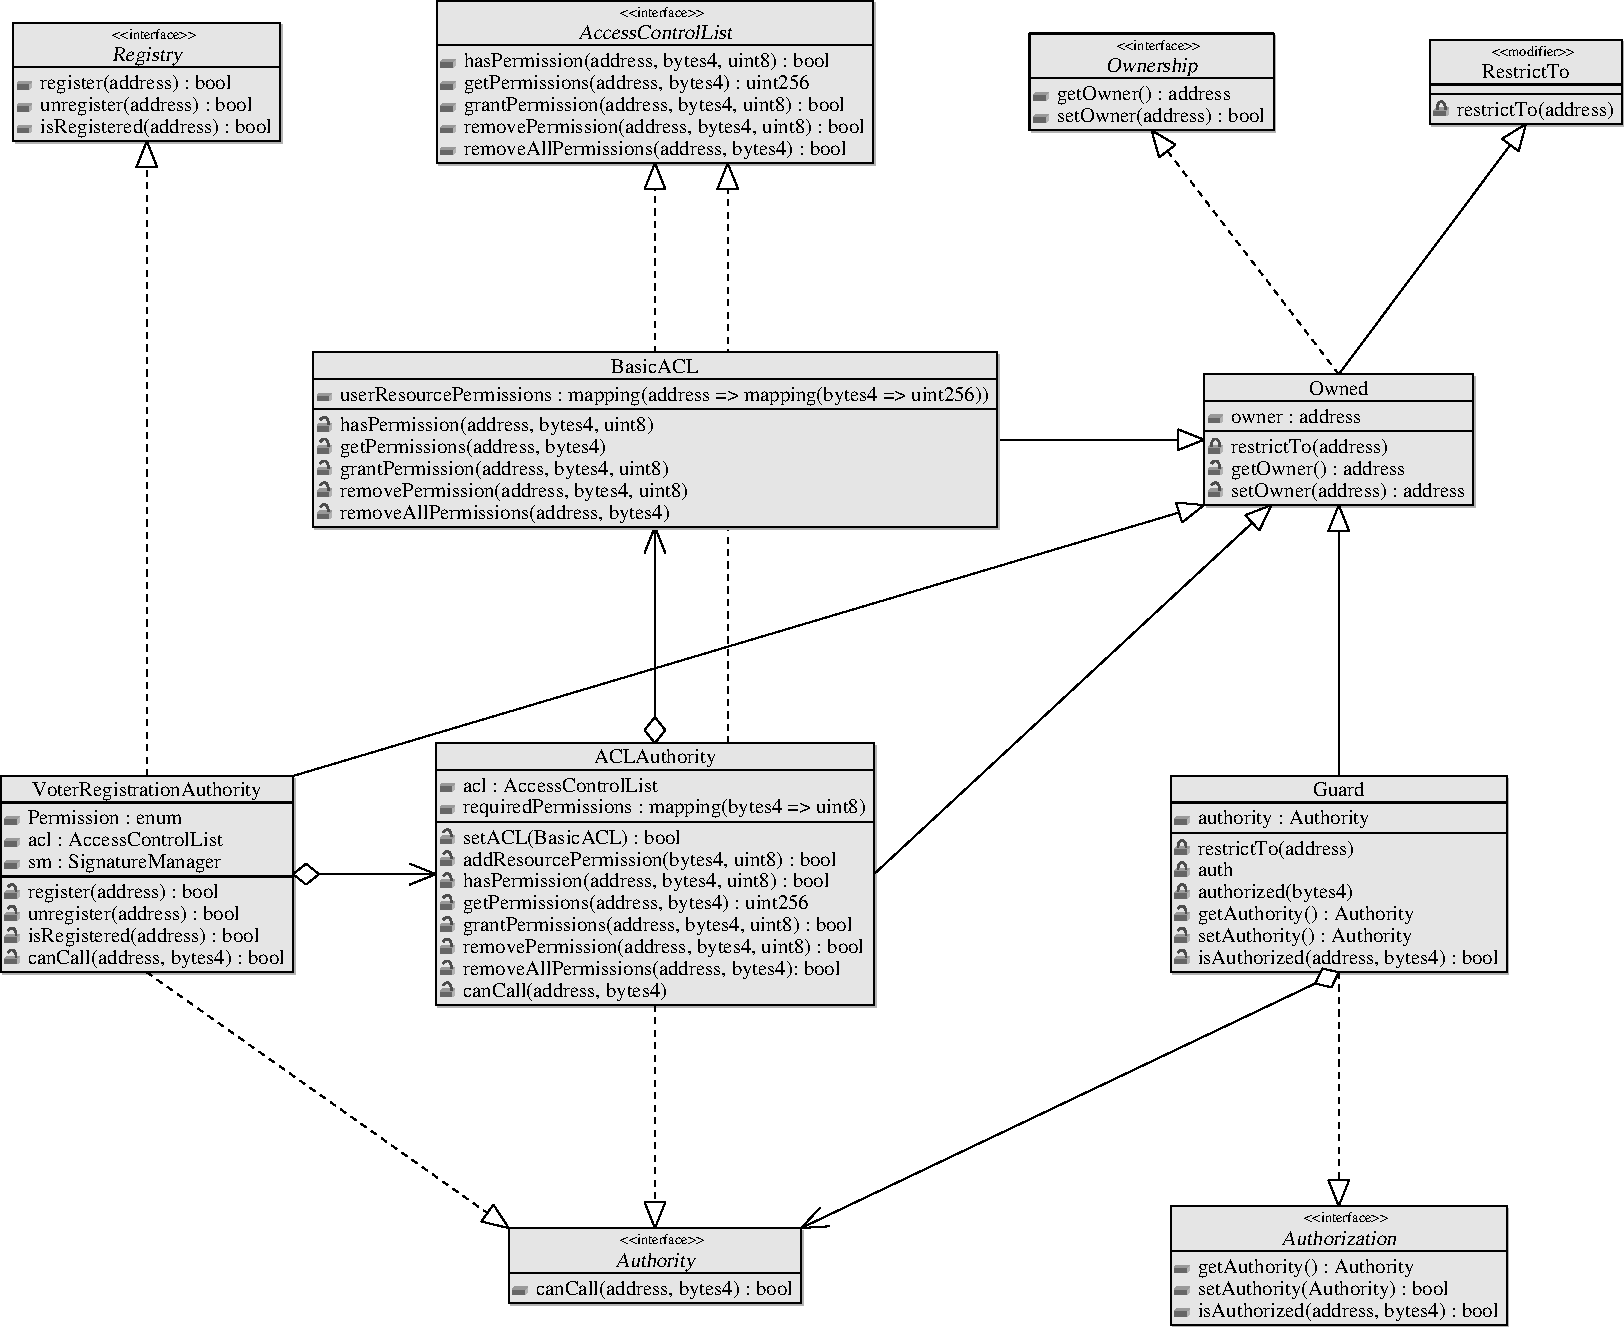
\includegraphics[width=\textwidth]{figures/authorization/figure}
%   % \includestandalone[width=\textwidth]{\fig{authorization}}
% \end{figure}

% \subsection{Finite State Machine}

% \subsection{First-Past-the-Post}
% The first-past-the-post \solt{contract} is the simplest election \solt{contract}
% implementation.

\subsection{Election Contracts}

\input{appendix/code/election/first-past-the-post}

% \subsubsection{Range Vote}
%
% \subsubsection{Single Transferable Vote}


% Section: Delegation Components
\section{Delegation Components}

This section explores the components relating to vote delegation. The delegation
components are responsible for managing the delegation of voters' votes to
delegates.

% \begin{figure}[H]
%   \centering
%   \caption{Authorization dependency graph modeling.}% \label{fig:authorization}
%   \figurepdf[width=\textwidth]{authorization}
%   % 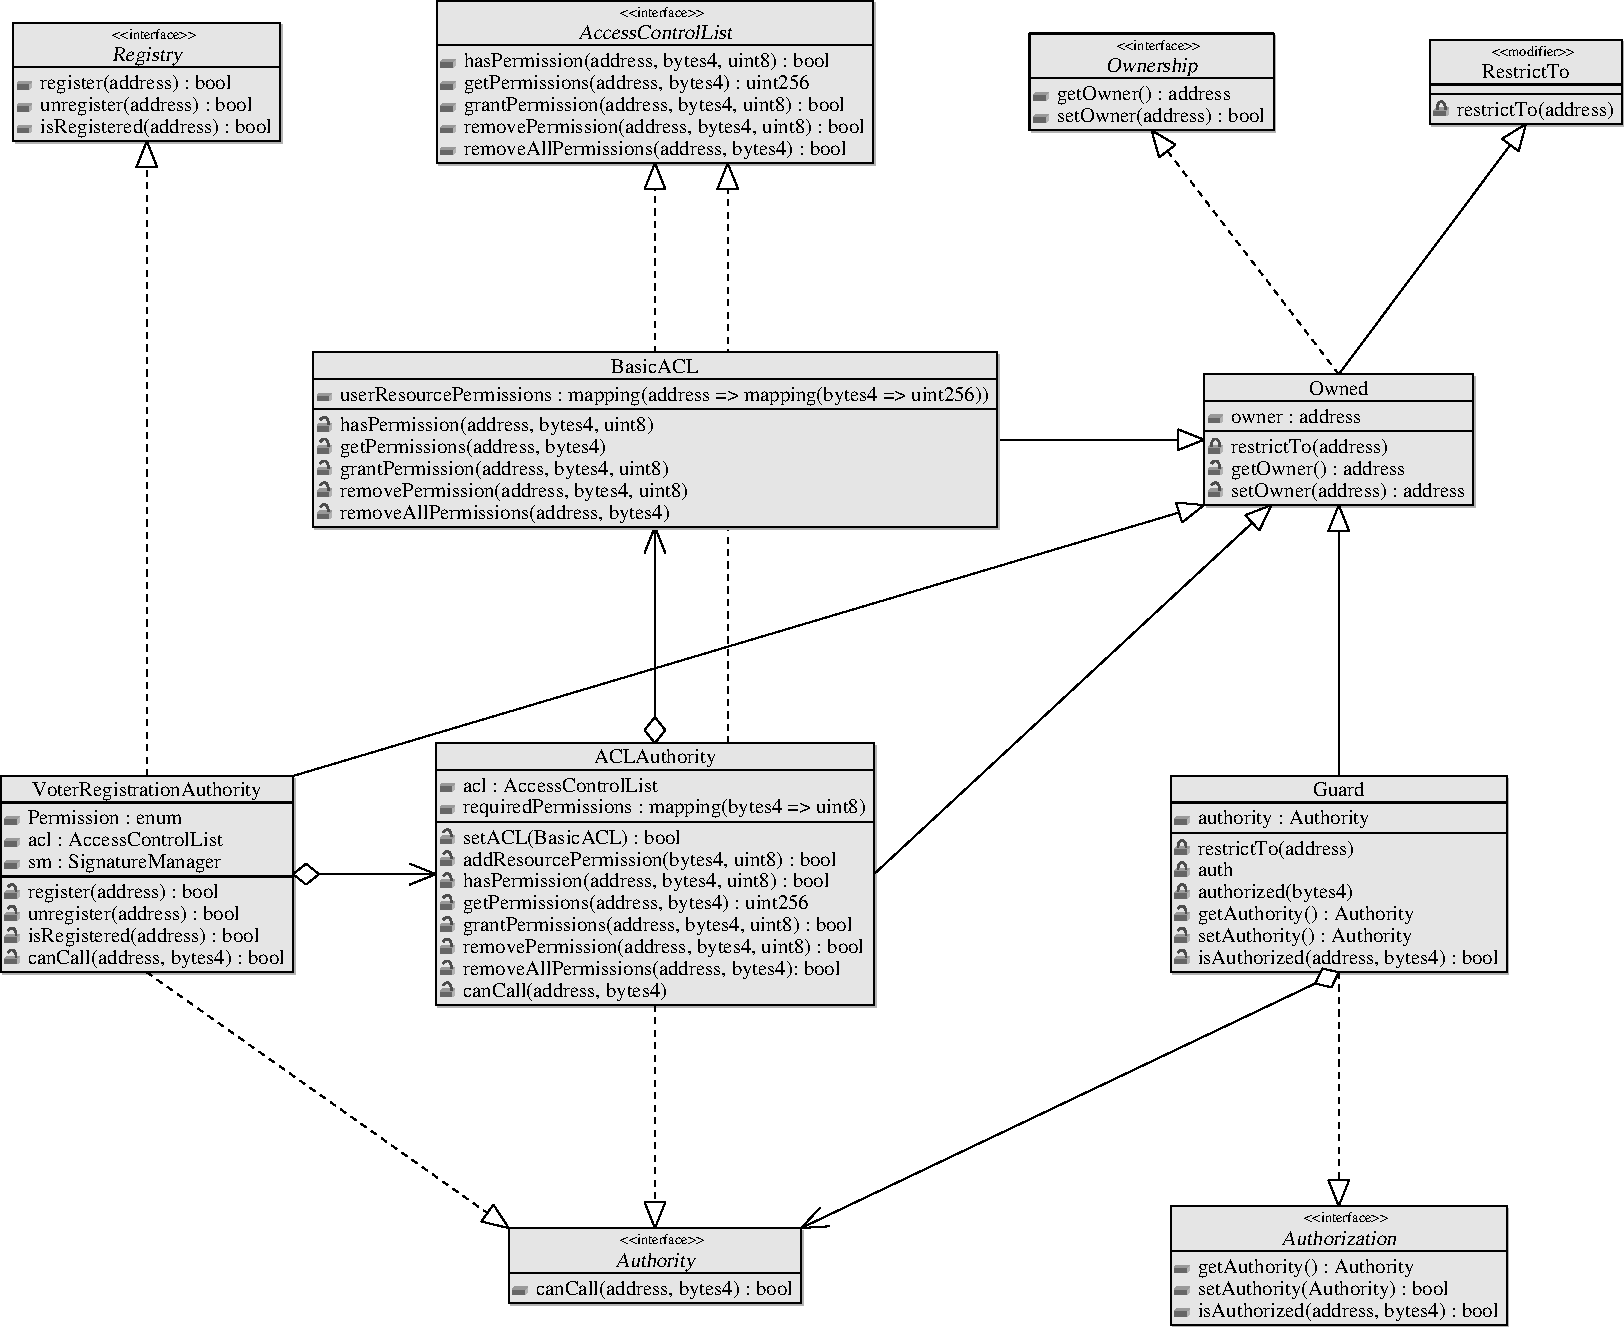
\includegraphics[width=\textwidth]{figures/authorization/figure}
%   % \includestandalone[width=\textwidth]{\fig{authorization}}
% \end{figure}

% Section: delegation
\input{appendix/code/delegation/delegation}


\end{appendices}
 % Start with '\chapter{Title}'
%You can always add more appendices here if you want

%-----------------------------------------------------------------------------%
% BIOGRAPHY -- Start file with '\biography'.  Mandatory for Ph.D.
%-----------------------------------------------------------------------------%
% \addcontentsline{toc}{chapter}{Vita}
\biography{}

Nathaniel Patrick Hernandez --- born in Memphis, Tennessee, to Alison and Juan
Hernandez --- developed a passion for technology and software at a young age
and has been passionately writing software and exploring the field of computer
science ever since. In 2012 Nathan earned his Associate of Science from Coastal
Carolina Community College. The next year, with barely the wherewithal to
attend a single semester, he began his Bachelor of Science at Appalachian State
University. Nathan was fortunate to have been noticed by the faculty of The
Department of Computer Science there and presented with opportunities to work
with faculty members in a variety of ways.

Dr.~Rahman Tashakkori in particular played a significant role in Nathan's
undergraduate degree, academic career, and personal life --- investing
significant amounts of time and energy which came in the shape of mentorship,
engaging academic problems, personal challenges, and friendship --- helping
Nathan to grow personally, academically, and eventually providing the
encouragement to pursue a Master's degree. Throughout Nathan's academic career
Dr.~Tashakkori presented him with scholarship and research opportunities;
allowing him, along with a team of other hand-picked students, to conduct
research, built software and hardware systems, publish results, and present
findings on the beehive monitoring and analytics systems they built together.
This research served as the foundation for Nathan's undergraduate thesis which
enabled him to earn his Bachelor of Science.

Outside of academia, Nathan spent just under a year interning with IBM's jStart
team, a small group within IBM's Emerging Technologies department responsible
for prototyping systems for clients which leveraged new and promising
technologies. Nathan spent a majority of his time there immersing himself in
the field of big-data analytics: exploring Apache Kafka, analyzing client data,
generating insights, and building real-time data-processing pipelines. Having a
strong interest in cybersecurity and cryptography, Nathan also spent a summer
in San Fransisco, California, interning at UnifyID, a startup whose goal is to
build advanced security, authentication, and password management solutions.
While there Nathan worked on building important components of UnifyID's Google
Chrome extension for password management and participated in launching their
private beta. A few months after the end of his internship UnifyID went on to
win runner-ups in the 2016 TechCrunch Disrupt Battlfield.

% and present
% results, and explore challenging unique ideas which eventually resulted in

% Your biography is limited to one page and must contain
% \begin{enumerate}
%     \normalbaselines{}
% \item Full name
% \item Date and place of birth
% \item Every degree you've earned, including this one, and where you earned it
%     from.
% \end{enumerate}
% Mostly, that information is to narrow down which John Smith wrote that
% dissertation on the mating habits of sea cucumbers.  Sexy!
%
% You may also include
% \begin{enumerate}
%     \item Any awards you've won related to your discipline since your
%         undergraduate degree.
%     \item Any fellowships you've held
%     \item Anything you've published (papers, books, book chapters).  Don't be
%         afraid to cite it here, so that the full bibliographic record of your
%         article appears in the bibliography!
%     \item Where your next job will be, if you know
% \end{enumerate}


% VITA
% David John Cholmondeley II was born in Florence, Italy, to David and Shelby
% Cholmondeley. He graduated from Andover Academy in Massachusetts in June 1992.
% The following autumn, he entered Manchester University to study History, and in
% June 1995 he was awarded the Bachelor of Arts degree. In the fall of 1995, he
% accepted a research assistantship in History at Appalachian State University
% and began study toward a Master of Arts degree. The M.A. was awarded in June
% 1997. In September 1997, Mr. Cholmondeley commenced work toward his Ph.D. in
% International Trade at Georgetown University.
%
% Mr. Cholmondeley is a member of Phi Kappa Phi and Alpha Epsilon Lambda, and
% remains active in scouting as a troop leader. He resides in Washington, D.C.
% with his wife and four children.


%-----------------------------------------------------------------------------
% You're done :)
\end{document}
